\documentclass[twoside]{book}

% Packages required by doxygen
\usepackage{fixltx2e}
\usepackage{calc}
\usepackage{doxygen}
\usepackage[export]{adjustbox} % also loads graphicx
\usepackage{graphicx}
\usepackage[utf8]{inputenc}
\usepackage{makeidx}
\usepackage{multicol}
\usepackage{multirow}
\PassOptionsToPackage{warn}{textcomp}
\usepackage{textcomp}
\usepackage[nointegrals]{wasysym}
\usepackage[table]{xcolor}

% NLS support packages
\usepackage{polski}
\usepackage[T1]{fontenc}

% Font selection
\usepackage[T1]{fontenc}
\usepackage[scaled=.90]{helvet}
\usepackage{courier}
\usepackage{amssymb}
\usepackage{sectsty}
\renewcommand{\familydefault}{\sfdefault}
\allsectionsfont{%
  \fontseries{bc}\selectfont%
  \color{darkgray}%
}
\renewcommand{\DoxyLabelFont}{%
  \fontseries{bc}\selectfont%
  \color{darkgray}%
}
\newcommand{\+}{\discretionary{\mbox{\scriptsize$\hookleftarrow$}}{}{}}

% Page & text layout
\usepackage{geometry}
\geometry{%
  a4paper,%
  top=2.5cm,%
  bottom=2.5cm,%
  left=2.5cm,%
  right=2.5cm%
}
\tolerance=750
\hfuzz=15pt
\hbadness=750
\setlength{\emergencystretch}{15pt}
\setlength{\parindent}{0cm}
\setlength{\parskip}{3ex plus 2ex minus 2ex}
\makeatletter
\renewcommand{\paragraph}{%
  \@startsection{paragraph}{4}{0ex}{-1.0ex}{1.0ex}{%
    \normalfont\normalsize\bfseries\SS@parafont%
  }%
}
\renewcommand{\subparagraph}{%
  \@startsection{subparagraph}{5}{0ex}{-1.0ex}{1.0ex}{%
    \normalfont\normalsize\bfseries\SS@subparafont%
  }%
}
\makeatother

% Headers & footers
\usepackage{fancyhdr}
\pagestyle{fancyplain}
\fancyhead[LE]{\fancyplain{}{\bfseries\thepage}}
\fancyhead[CE]{\fancyplain{}{}}
\fancyhead[RE]{\fancyplain{}{\bfseries\leftmark}}
\fancyhead[LO]{\fancyplain{}{\bfseries\rightmark}}
\fancyhead[CO]{\fancyplain{}{}}
\fancyhead[RO]{\fancyplain{}{\bfseries\thepage}}
\fancyfoot[LE]{\fancyplain{}{}}
\fancyfoot[CE]{\fancyplain{}{}}
\fancyfoot[RE]{\fancyplain{}{\bfseries\scriptsize Wygenerowano przez Doxygen }}
\fancyfoot[LO]{\fancyplain{}{\bfseries\scriptsize Wygenerowano przez Doxygen }}
\fancyfoot[CO]{\fancyplain{}{}}
\fancyfoot[RO]{\fancyplain{}{}}
\renewcommand{\footrulewidth}{0.4pt}
\renewcommand{\chaptermark}[1]{%
  \markboth{#1}{}%
}
\renewcommand{\sectionmark}[1]{%
  \markright{\thesection\ #1}%
}

% Indices & bibliography
\usepackage{natbib}
\usepackage[titles]{tocloft}
\setcounter{tocdepth}{3}
\setcounter{secnumdepth}{5}
\makeindex

% Hyperlinks (required, but should be loaded last)
\usepackage{ifpdf}
\ifpdf
  \usepackage[pdftex,pagebackref=true]{hyperref}
\else
  \usepackage[ps2pdf,pagebackref=true]{hyperref}
\fi
\hypersetup{%
  colorlinks=true,%
  linkcolor=blue,%
  citecolor=blue,%
  unicode%
}

% Custom commands
\newcommand{\clearemptydoublepage}{%
  \newpage{\pagestyle{empty}\cleardoublepage}%
}

\usepackage{caption}
\captionsetup{labelsep=space,justification=centering,font={bf},singlelinecheck=off,skip=4pt,position=top}

%===== C O N T E N T S =====

\begin{document}

% Titlepage & ToC
\hypersetup{pageanchor=false,
             bookmarksnumbered=true,
             pdfencoding=unicode
            }
\pagenumbering{alph}
\begin{titlepage}
\vspace*{7cm}
\begin{center}%
{\Large Dron Podwodny II }\\
\vspace*{1cm}
{\large Wygenerowano przez Doxygen 1.8.13}\\
\end{center}
\end{titlepage}
\clearemptydoublepage
\pagenumbering{roman}
\tableofcontents
\clearemptydoublepage
\pagenumbering{arabic}
\hypersetup{pageanchor=true}

%--- Begin generated contents ---
\chapter{Indeks przestrzeni nazw}
\section{Lista przestrzeni nazw}
Tutaj znajdują się wszystkie udokumentowane przestrzenie nazw wraz z ich krótkimi opisami\+:\begin{DoxyCompactList}
\item\contentsline{section}{\hyperlink{namespacePzG}{PzG} \\*Moduł narzędzi umożliwiających połącznie z G\+N\+U\+Plotem }{\pageref{namespacePzG}}{}
\end{DoxyCompactList}

\chapter{Indeks hierarchiczny}
\section{Hierarchia klas}
Ta lista dziedziczenia posortowana jest z grubsza, choć nie całkowicie, alfabetycznie\+:\begin{DoxyCompactList}
\item \contentsline{section}{Dron}{\pageref{classDron}}{}
\item \contentsline{section}{PzG\+:\+:Info\+Pliku\+Do\+Rysowania}{\pageref{classPzG_1_1InfoPlikuDoRysowania}}{}
\item \contentsline{section}{PzG\+:\+:Lacze\+Do\+G\+N\+U\+Plota}{\pageref{classPzG_1_1LaczeDoGNUPlota}}{}
\item \contentsline{section}{Obiekt\+Sceny}{\pageref{classObiektSceny}}{}
\begin{DoxyCompactList}
\item \contentsline{section}{Graniastoslup}{\pageref{classGraniastoslup}}{}
\begin{DoxyCompactList}
\item \contentsline{section}{Graniastoslup\+S\+CN}{\pageref{classGraniastoslupSCN}}{}
\end{DoxyCompactList}
\item \contentsline{section}{Powierzchnia}{\pageref{classPowierzchnia}}{}
\item \contentsline{section}{Powierzchnia\+Falowana}{\pageref{classPowierzchniaFalowana}}{}
\item \contentsline{section}{Pret}{\pageref{classPret}}{}
\item \contentsline{section}{Prostopadloscian}{\pageref{classProstopadloscian}}{}
\begin{DoxyCompactList}
\item \contentsline{section}{Prostopadloscian\+S\+CN}{\pageref{classProstopadloscianSCN}}{}
\end{DoxyCompactList}
\end{DoxyCompactList}
\item \contentsline{section}{Scena}{\pageref{classScena}}{}
\item \contentsline{section}{S\+Macierz$<$ Typ, Wymiar $>$}{\pageref{classSMacierz}}{}
\item \contentsline{section}{S\+Wektor$<$ Typ, Wymiar $>$}{\pageref{classSWektor}}{}
\item \contentsline{section}{S\+Wektor$<$ double, 3 $>$}{\pageref{classSWektor}}{}
\end{DoxyCompactList}

\chapter{Indeks klas}
\section{Lista klas}
Tutaj znajdują się klasy, struktury, unie i interfejsy wraz z ich krótkimi opisami\+:\begin{DoxyCompactList}
\item\contentsline{section}{\hyperlink{classDron}{Dron} \\*Definicja klasy \hyperlink{classDron}{Dron} }{\pageref{classDron}}{}
\item\contentsline{section}{\hyperlink{classGraniastoslup}{Graniastoslup} \\*\hyperlink{classGraniastoslup}{Graniastoslup} jako bryla przestrzenna o promieniu i srodku lokalnym }{\pageref{classGraniastoslup}}{}
\item\contentsline{section}{\hyperlink{classGraniastoslupSCN}{Graniastoslup\+S\+CN} \\*\hyperlink{classGraniastoslupSCN}{Graniastoslup\+S\+CN} jako \hyperlink{classGraniastoslup}{Graniastoslup} w ukladzie globalnym }{\pageref{classGraniastoslupSCN}}{}
\item\contentsline{section}{\hyperlink{classPzG_1_1InfoPlikuDoRysowania}{Pz\+G\+::\+Info\+Pliku\+Do\+Rysowania} \\*Zestaw informacji dotyczący pliku i sposobu rysowania }{\pageref{classPzG_1_1InfoPlikuDoRysowania}}{}
\item\contentsline{section}{\hyperlink{classPzG_1_1LaczeDoGNUPlota}{Pz\+G\+::\+Lacze\+Do\+G\+N\+U\+Plota} \\*Klasa realizuje interfejs do programu G\+N\+U\+Plot }{\pageref{classPzG_1_1LaczeDoGNUPlota}}{}
\item\contentsline{section}{\hyperlink{classObiektSceny}{Obiekt\+Sceny} \\*Definicja klasy \hyperlink{classObiektSceny}{Obiekt\+Sceny} }{\pageref{classObiektSceny}}{}
\item\contentsline{section}{\hyperlink{classPowierzchnia}{Powierzchnia} \\*\hyperlink{classPowierzchnia}{Powierzchnia} jako obiekt graficzny }{\pageref{classPowierzchnia}}{}
\item\contentsline{section}{\hyperlink{classPowierzchniaFalowana}{Powierzchnia\+Falowana} \\*\hyperlink{classPowierzchniaFalowana}{Powierzchnia\+Falowana} jako obiekt graficzny }{\pageref{classPowierzchniaFalowana}}{}
\item\contentsline{section}{\hyperlink{classPret}{Pret} \\*\hyperlink{classPret}{Pret} jako obiekt graficzny }{\pageref{classPret}}{}
\item\contentsline{section}{\hyperlink{classProstopadloscian}{Prostopadloscian} \\*\hyperlink{classProstopadloscian}{Prostopadloscian} jako bryla przestrzenna o promieniu i srodku lokalnym }{\pageref{classProstopadloscian}}{}
\item\contentsline{section}{\hyperlink{classProstopadloscianSCN}{Prostopadloscian\+S\+CN} \\*\hyperlink{classProstopadloscianSCN}{Prostopadloscian\+S\+CN} jako \hyperlink{classProstopadloscian}{Prostopadloscian} w ukladzie globalnym }{\pageref{classProstopadloscianSCN}}{}
\item\contentsline{section}{\hyperlink{classScena}{Scena} \\*\hyperlink{classScena}{Scena} jako klasa zarzadzajaca obiektami graficznymi }{\pageref{classScena}}{}
\item\contentsline{section}{\hyperlink{classSMacierz}{S\+Macierz$<$ Typ, Wymiar $>$} \\*Klasa modeluje pojęcie macierzy kwadratowej }{\pageref{classSMacierz}}{}
\item\contentsline{section}{\hyperlink{classSWektor}{S\+Wektor$<$ Typ, Wymiar $>$} \\*Klasa modeluje pojecie wektora }{\pageref{classSWektor}}{}
\end{DoxyCompactList}

\chapter{Indeks plików}
\section{Lista plików}
Tutaj znajduje się lista wszystkich udokumentowanych plików z ich krótkimi opisami\+:\begin{DoxyCompactList}
\item\contentsline{section}{inc/\hyperlink{Dron_8hh}{Dron.\+hh} \\*Zawiera definicję klasy \hyperlink{classDron}{Dron} }{\pageref{Dron_8hh}}{}
\item\contentsline{section}{inc/\hyperlink{Graniastoslup_8hh}{Graniastoslup.\+hh} \\*Zawiera definicję klasy \hyperlink{classGraniastoslup}{Graniastoslup} }{\pageref{Graniastoslup_8hh}}{}
\item\contentsline{section}{inc/\hyperlink{GraniastoslupSCN_8hh}{Graniastoslup\+S\+C\+N.\+hh} \\*Zawiera definicję klasy \hyperlink{classGraniastoslupSCN}{Graniastoslup\+S\+CN} }{\pageref{GraniastoslupSCN_8hh}}{}
\item\contentsline{section}{inc/\hyperlink{lacze__do__gnuplota_8hh}{lacze\+\_\+do\+\_\+gnuplota.\+hh} \\*Zawiera definicję klasy \hyperlink{classPzG_1_1LaczeDoGNUPlota}{Pz\+G\+::\+Lacze\+Do\+G\+N\+U\+Plota} }{\pageref{lacze__do__gnuplota_8hh}}{}
\item\contentsline{section}{inc/\hyperlink{ObiektSceny_8hh}{Obiekt\+Sceny.\+hh} \\*Zawiera definicję klasy \hyperlink{classObiektSceny}{Obiekt\+Sceny} }{\pageref{ObiektSceny_8hh}}{}
\item\contentsline{section}{inc/\hyperlink{Powierzchnia_8hh}{Powierzchnia.\+hh} \\*Zawiera definicję klasy \hyperlink{classPowierzchnia}{Powierzchnia} }{\pageref{Powierzchnia_8hh}}{}
\item\contentsline{section}{inc/\hyperlink{PowierzchniaFalowana_8hh}{Powierzchnia\+Falowana.\+hh} \\*Zawiera definicję klasy \hyperlink{classPowierzchniaFalowana}{Powierzchnia\+Falowana} }{\pageref{PowierzchniaFalowana_8hh}}{}
\item\contentsline{section}{inc/\hyperlink{Pret_8hh}{Pret.\+hh} \\*Zawiera definicję klasy \hyperlink{classPret}{Pret} }{\pageref{Pret_8hh}}{}
\item\contentsline{section}{inc/\hyperlink{Prostopadloscian_8hh}{Prostopadloscian.\+hh} \\*Zawiera definicję klasy \hyperlink{classProstopadloscian}{Prostopadloscian} }{\pageref{Prostopadloscian_8hh}}{}
\item\contentsline{section}{inc/\hyperlink{ProstopadloscianSCN_8hh}{Prostopadloscian\+S\+C\+N.\+hh} \\*Zawiera definicję klasy \hyperlink{classProstopadloscianSCN}{Prostopadloscian\+S\+CN} }{\pageref{ProstopadloscianSCN_8hh}}{}
\item\contentsline{section}{inc/\hyperlink{Scena_8hh}{Scena.\+hh} \\*Zawiera definicję klasy \hyperlink{classScena}{Scena} }{\pageref{Scena_8hh}}{}
\item\contentsline{section}{inc/\hyperlink{SMacierz_8hh}{S\+Macierz.\+hh} \\*Plik zawiera definicje szablonu macierzy kwadratowej }{\pageref{SMacierz_8hh}}{}
\item\contentsline{section}{inc/\hyperlink{SWektor_8hh}{S\+Wektor.\+hh} \\*Plik zawiera szablon klasy modelujacej pojecie wektora }{\pageref{SWektor_8hh}}{}
\item\contentsline{section}{inc/\hyperlink{typy__danych_8hh}{typy\+\_\+danych.\+hh} \\*Zawiera definicję Wektora3D oraz Macierzy3x3 }{\pageref{typy__danych_8hh}}{}
\item\contentsline{section}{src/\hyperlink{Dron_8cpp}{Dron.\+cpp} \\*Zawiera definicje dluzszych metod klasy \hyperlink{classDron}{Dron} }{\pageref{Dron_8cpp}}{}
\item\contentsline{section}{src/\hyperlink{Graniastoslup_8cpp}{Graniastoslup.\+cpp} \\*Zawiera definicje dluzszych metod klasy \hyperlink{classGraniastoslup}{Graniastoslup} }{\pageref{Graniastoslup_8cpp}}{}
\item\contentsline{section}{src/\hyperlink{GraniastoslupSCN_8cpp}{Graniastoslup\+S\+C\+N.\+cpp} \\*Zawiera definicje dluzszych metod klasy \hyperlink{classGraniastoslupSCN}{Graniastoslup\+S\+CN} }{\pageref{GraniastoslupSCN_8cpp}}{}
\item\contentsline{section}{src/\hyperlink{lacze__do__gnuplota_8cpp}{lacze\+\_\+do\+\_\+gnuplota.\+cpp} \\*Zawiera definicje metod klasy Lacze\+Do\+G\+N\+U\+Plota }{\pageref{lacze__do__gnuplota_8cpp}}{}
\item\contentsline{section}{src/\hyperlink{main_8cpp}{main.\+cpp} \\*Zawiera funkcje main }{\pageref{main_8cpp}}{}
\item\contentsline{section}{src/\hyperlink{Powierzchnia_8cpp}{Powierzchnia.\+cpp} \\*Zawiera definicje dluzszych metod klasy \hyperlink{classPowierzchnia}{Powierzchnia} }{\pageref{Powierzchnia_8cpp}}{}
\item\contentsline{section}{src/\hyperlink{PowierzchniaFalowana_8cpp}{Powierzchnia\+Falowana.\+cpp} \\*Zawiera definicje dluzszych metod klasy \hyperlink{classPowierzchniaFalowana}{Powierzchnia\+Falowana} }{\pageref{PowierzchniaFalowana_8cpp}}{}
\item\contentsline{section}{src/\hyperlink{Pret_8cpp}{Pret.\+cpp} \\*Zawiera definicje dluzszych metod klasy \hyperlink{classPret}{Pret} }{\pageref{Pret_8cpp}}{}
\item\contentsline{section}{src/\hyperlink{Prostopadloscian_8cpp}{Prostopadloscian.\+cpp} \\*Zawiera definicje dluzszych metod klasy \hyperlink{classProstopadloscian}{Prostopadloscian} }{\pageref{Prostopadloscian_8cpp}}{}
\item\contentsline{section}{src/\hyperlink{ProstopadloscianSCN_8cpp}{Prostopadloscian\+S\+C\+N.\+cpp} \\*Zawiera definicje dluzszych metod klasy \hyperlink{classProstopadloscianSCN}{Prostopadloscian\+S\+CN} }{\pageref{ProstopadloscianSCN_8cpp}}{}
\item\contentsline{section}{src/\hyperlink{Scena_8cpp}{Scena.\+cpp} \\*Zawiera definicje dluzszych metod klasy \hyperlink{classScena}{Scena} }{\pageref{Scena_8cpp}}{}
\end{DoxyCompactList}

\chapter{Dokumentacja przestrzeni nazw}
\hypertarget{namespacePzG}{}\section{Dokumentacja przestrzeni nazw PzG}
\label{namespacePzG}\index{PzG@{PzG}}


Moduł narzędzi umożliwiających połącznie z G\+N\+U\+Plotem.  


\subsection*{Komponenty}
\begin{DoxyCompactItemize}
\item 
class \hyperlink{classPzG_1_1InfoPlikuDoRysowania}{Info\+Pliku\+Do\+Rysowania}
\begin{DoxyCompactList}\small\item\em Zestaw informacji dotyczący pliku i sposobu rysowania. \end{DoxyCompactList}\item 
class \hyperlink{classPzG_1_1LaczeDoGNUPlota}{Lacze\+Do\+G\+N\+U\+Plota}
\begin{DoxyCompactList}\small\item\em Klasa realizuje interfejs do programu G\+N\+U\+Plot. \end{DoxyCompactList}\end{DoxyCompactItemize}
\subsection*{Wyliczenia}
\begin{DoxyCompactItemize}
\item 
enum \hyperlink{namespacePzG_aeedae1ef10c66d720f9e89de408ca4ca}{Tryb\+Rysowania} \{ {\bfseries T\+R\+\_\+2D}, 
{\bfseries T\+R\+\_\+3D}
 \}\begin{DoxyCompactList}\small\item\em Określa tryb rysowania realizowanego przez program {\ttfamily gnuplot}. \end{DoxyCompactList}
\item 
enum \hyperlink{namespacePzG_a705c92106f39b7d0c34a6739d10ff0b6}{Rodzaj\+Rysowania} \{ {\bfseries R\+R\+\_\+\+Ciagly}, 
{\bfseries R\+R\+\_\+\+Punktowy}
 \}\begin{DoxyCompactList}\small\item\em Sposób rysowania linii. \end{DoxyCompactList}
\end{DoxyCompactItemize}
\subsection*{Funkcje}
\begin{DoxyCompactItemize}
\item 
\mbox{\Hypertarget{namespacePzG_ae1ae4d36f66c77879380ba73da8e20e3}\label{namespacePzG_ae1ae4d36f66c77879380ba73da8e20e3}} 
bool {\bfseries Czy\+Jest\+Plik} (char const $\ast$Nazwa\+Pliku)
\end{DoxyCompactItemize}


\subsection{Opis szczegółowy}
Moduł narzędzi umożliwiających połącznie z G\+N\+U\+Plotem. 

Niniejsza przestrzeń nazw stanowi moduł logiczny zawierający narzędzia umożliwiające realizację połączenia z programem {\ttfamily gnuplot}. 

\subsection{Dokumentacja typów wyliczanych}
\mbox{\Hypertarget{namespacePzG_a705c92106f39b7d0c34a6739d10ff0b6}\label{namespacePzG_a705c92106f39b7d0c34a6739d10ff0b6}} 
\index{PzG@{PzG}!Rodzaj\+Rysowania@{Rodzaj\+Rysowania}}
\index{Rodzaj\+Rysowania@{Rodzaj\+Rysowania}!PzG@{PzG}}
\subsubsection{\texorpdfstring{Rodzaj\+Rysowania}{RodzajRysowania}}
{\footnotesize\ttfamily enum \hyperlink{namespacePzG_a705c92106f39b7d0c34a6739d10ff0b6}{Pz\+G\+::\+Rodzaj\+Rysowania}}



Sposób rysowania linii. 

Określa sposób rysowania linii. \mbox{\Hypertarget{namespacePzG_aeedae1ef10c66d720f9e89de408ca4ca}\label{namespacePzG_aeedae1ef10c66d720f9e89de408ca4ca}} 
\index{PzG@{PzG}!Tryb\+Rysowania@{Tryb\+Rysowania}}
\index{Tryb\+Rysowania@{Tryb\+Rysowania}!PzG@{PzG}}
\subsubsection{\texorpdfstring{Tryb\+Rysowania}{TrybRysowania}}
{\footnotesize\ttfamily enum \hyperlink{namespacePzG_aeedae1ef10c66d720f9e89de408ca4ca}{Pz\+G\+::\+Tryb\+Rysowania}}



Określa tryb rysowania realizowanego przez program {\ttfamily gnuplot}. 

Typ wyliczeniowy określające dopuszczalne tryby rysowania realizowanego przez program {\ttfamily gnuplot}. Wybór trybu wiąże się ze zmianą sposobu interpretacji danych zawartych pliku. Jeśli np. wybrany zostanie tryb 2D, to zakłada się, że w każdej linii pliku z danymi znajdują się wartości współrzędnych {\itshape x}, {\itshape y}. Wartości typu\+: \begin{DoxyItemize}
\item {\ttfamily T\+R\+\_\+2D} -\/ rysowanie w trybie 2D, co sprowadza się do rysowania wykresów funkcji jednej zmiennej. \item {\ttfamily T\+R\+\_\+3D} -\/ rysowanie w trybie 3D. Oznacza to możliwość rysowania wykresów funkcji dwóch zmiennych. \end{DoxyItemize}

\chapter{Dokumentacja klas}
\hypertarget{classDron}{}\section{Dokumentacja klasy Dron}
\label{classDron}\index{Dron@{Dron}}


Definicja klasy \hyperlink{classDron}{Dron}.  




{\ttfamily \#include $<$Dron.\+hh$>$}



Diagram współpracy dla Dron\+:
\nopagebreak
\begin{figure}[H]
\begin{center}
\leavevmode
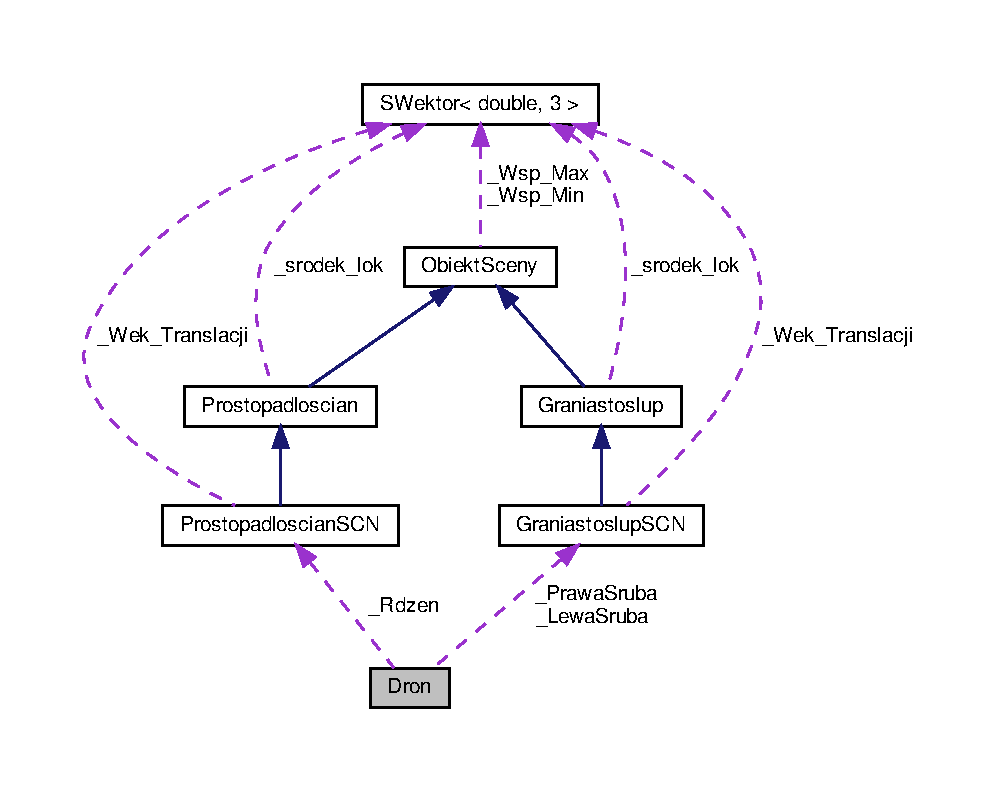
\includegraphics[width=350pt]{classDron__coll__graph}
\end{center}
\end{figure}
\subsection*{Metody publiczne}
\begin{DoxyCompactItemize}
\item 
\hyperlink{classProstopadloscianSCN}{Prostopadloscian\+S\+CN} \& \hyperlink{classDron_addd3f76aedda33de1c13d7a0cd5bea69}{Wez\+\_\+\+Rdzen} ()
\begin{DoxyCompactList}\small\item\em Metoda umozliwia zewnetrzne odnoszenie sie do obiektu skladowego \+\_\+\+Rdzen. \end{DoxyCompactList}\item 
\hyperlink{classGraniastoslupSCN}{Graniastoslup\+S\+CN} \& \hyperlink{classDron_a18b1d0162c88a8e93322d6eb5d7b64f0}{Wez\+\_\+\+Lewa\+\_\+\+Srube} ()
\begin{DoxyCompactList}\small\item\em Metoda umozliwia zewnetrzne odnoszenie sie do obiektu skladowego \+\_\+\+Lewa\+Sruba. \end{DoxyCompactList}\item 
\hyperlink{classGraniastoslupSCN}{Graniastoslup\+S\+CN} \& \hyperlink{classDron_a1bdfbac069ae0f0ef1b168f0f2d9bc6e}{Wez\+\_\+\+Prawa\+\_\+\+Srube} ()
\begin{DoxyCompactList}\small\item\em Metoda umozliwia zewnetrzne odnoszenie sie do obiektu skladowego \+\_\+\+Prawa\+Sruba. \end{DoxyCompactList}\item 
bool \hyperlink{classDron_a5ddaabc5c441d8f2f204cc398e1b0db2}{Sprawdz\+Mozliwosc\+Ruchu} (\hyperlink{classObiektSceny}{Obiekt\+Sceny} \&obiekt)
\begin{DoxyCompactList}\small\item\em Metoda umozliwia sprawdzenie mozliwosci wystapienia kolizji drona z przeszkoda. \end{DoxyCompactList}\item 
void \hyperlink{classDron_a75782b1ce9cd9f911e45f87f75ae95d6}{Zmien\+\_\+o\+\_\+kat} (unsigned int kat)
\begin{DoxyCompactList}\small\item\em Metoda umozliwia zmiane orientacji drona wokol osi OZ. \end{DoxyCompactList}\item 
void \hyperlink{classDron_a6fcd15ec24881f0e92e84fc04ddd9a9a}{Zmien\+\_\+o\+\_\+kat\+\_\+wlasny} (unsigned int kat)
\begin{DoxyCompactList}\small\item\em Metoda umozliwia zmiane orientacji srub wokol osi OX. \end{DoxyCompactList}\item 
void \hyperlink{classDron_a5f5867d7f7adb7e540ef762a782a4103}{Zmien\+\_\+o\+\_\+translacje} (\hyperlink{classSWektor}{Wektor3D} Translacja)
\begin{DoxyCompactList}\small\item\em Metoda umozliwia zmiane polozenia drona. \end{DoxyCompactList}\item 
bool \hyperlink{classDron_ac0c17bd50d8f7c11457ab69cb2237abb}{Oblicz\+Globalne} () const
\begin{DoxyCompactList}\small\item\em Realizuje przeksztalcenie wspolrzednych lokalnych drona do ukladu globalnego. \end{DoxyCompactList}\end{DoxyCompactItemize}
\subsection*{Metody prywatne}
\begin{DoxyCompactItemize}
\item 
bool \hyperlink{classDron_a0d88b00af782f5e914887b2b089e1b9c}{Sprawdz\+Mozliwosc\+Ruchu\+Sruby} (\hyperlink{classObiektSceny}{Obiekt\+Sceny} \&obiekt, \hyperlink{classGraniastoslupSCN}{Graniastoslup\+S\+CN} \&sruba)
\begin{DoxyCompactList}\small\item\em Metoda umozliwia sprawdzenie mozliwosci wystapienia kolizji sruby z przeszkoda. \end{DoxyCompactList}\item 
bool \hyperlink{classDron_a4cff7a2c46fe43e32df58c8245d9d0d3}{Sprawdz\+Mozliwosc\+Ruchu\+Rdzenia} (\hyperlink{classObiektSceny}{Obiekt\+Sceny} \&obiekt)
\begin{DoxyCompactList}\small\item\em Metoda umozliwia sprawdzenie mozliwosci wystapienia kolizji rdzenia z przeszkoda. \end{DoxyCompactList}\end{DoxyCompactItemize}
\subsection*{Atrybuty prywatne}
\begin{DoxyCompactItemize}
\item 
\hyperlink{classProstopadloscianSCN}{Prostopadloscian\+S\+CN} \hyperlink{classDron_af62e07b9d016168d5a129515f65f1609}{\+\_\+\+Rdzen}
\begin{DoxyCompactList}\small\item\em Pole przechowuje rdzen drona. \end{DoxyCompactList}\item 
\hyperlink{classGraniastoslupSCN}{Graniastoslup\+S\+CN} \hyperlink{classDron_a16ece01f1022ab49f1017f010db254b1}{\+\_\+\+Lewa\+Sruba}
\begin{DoxyCompactList}\small\item\em Pole przechowuje lewa srube drona. \end{DoxyCompactList}\item 
\hyperlink{classGraniastoslupSCN}{Graniastoslup\+S\+CN} \hyperlink{classDron_abcf5121c081a80ec44fbfe1de9784f1d}{\+\_\+\+Prawa\+Sruba}
\begin{DoxyCompactList}\small\item\em Pole przechowuje prawa srube drona. \end{DoxyCompactList}\end{DoxyCompactItemize}


\subsection{Opis szczegółowy}
Definicja klasy \hyperlink{classDron}{Dron}. 

Definicja klasy \hyperlink{classDron}{Dron}, sluzacej do interpretacji zadanego obiektu jako drona zdolnego do bycia przemieszczonym i obroconym z poziomu metod sceny. Elementami skladowymi drona sa obiekty klasy \hyperlink{classGraniastoslupSCN}{Graniastoslup\+S\+CN} oznaczajace sruby oraz jeden obiekt klasy \hyperlink{classProstopadloscianSCN}{Prostopadloscian\+S\+CN} oznaczajacy rdzen drona. \hyperlink{classDron}{Dron} ponadto jest w stanie wykryc kolizje z dostarczonym mu obiektem klasy \hyperlink{classObiektSceny}{Obiekt\+Sceny} 

\subsection{Dokumentacja funkcji składowych}
\mbox{\Hypertarget{classDron_ac0c17bd50d8f7c11457ab69cb2237abb}\label{classDron_ac0c17bd50d8f7c11457ab69cb2237abb}} 
\index{Dron@{Dron}!Oblicz\+Globalne@{Oblicz\+Globalne}}
\index{Oblicz\+Globalne@{Oblicz\+Globalne}!Dron@{Dron}}
\subsubsection{\texorpdfstring{Oblicz\+Globalne()}{ObliczGlobalne()}}
{\footnotesize\ttfamily bool Dron\+::\+Oblicz\+Globalne (\begin{DoxyParamCaption}{ }\end{DoxyParamCaption}) const}



Realizuje przeksztalcenie wspolrzednych lokalnych drona do ukladu globalnego. 

Realizuje przeksztalcenie wspolrzednych lokalnych kazdego z elementow skladowych drona do ukladu globalnego biorac pod uwage ich kat orientacji oraz wektory translacji

\begin{DoxyPrecond}{Warunek wstępny}
Obiekty musza byc poprawnie zainicjalizowane 
\end{DoxyPrecond}

\begin{DoxyRetVals}{Zwracane wartości}
{\em true} & -\/ operacja przebiegla pomyslnie \\
\hline
{\em false} & -\/ nie udalo sie okreslic wspolrzednych globalnych -\/ dla przynajmniej jednego obiektu wystapil blad prawidlowego odczytania wspolrzednych z pliku {\itshape \+\_\+\+Plik\+\_\+\+Wsp\+\_\+\+Lokalne} lub blad zapisu do pliku {\itshape \+\_\+\+Plik\+\_\+\+Wsp\+\_\+\+Globalne} \\
\hline
\end{DoxyRetVals}
\mbox{\Hypertarget{classDron_a5ddaabc5c441d8f2f204cc398e1b0db2}\label{classDron_a5ddaabc5c441d8f2f204cc398e1b0db2}} 
\index{Dron@{Dron}!Sprawdz\+Mozliwosc\+Ruchu@{Sprawdz\+Mozliwosc\+Ruchu}}
\index{Sprawdz\+Mozliwosc\+Ruchu@{Sprawdz\+Mozliwosc\+Ruchu}!Dron@{Dron}}
\subsubsection{\texorpdfstring{Sprawdz\+Mozliwosc\+Ruchu()}{SprawdzMozliwoscRuchu()}}
{\footnotesize\ttfamily bool Dron\+::\+Sprawdz\+Mozliwosc\+Ruchu (\begin{DoxyParamCaption}\item[{\hyperlink{classObiektSceny}{Obiekt\+Sceny} \&}]{obiekt }\end{DoxyParamCaption})}



Metoda umozliwia sprawdzenie mozliwosci wystapienia kolizji drona z przeszkoda. 

Metoda umozliwia wykrycie kolizji drona z przeszkoda, wykorzystujac w tym celu metody prywatne \hyperlink{}{Dron\+:\+Sprawdz\+Mozliwosc\+Ruchu\+Sruby} i \hyperlink{classDron_a4cff7a2c46fe43e32df58c8245d9d0d3}{Dron\+::\+Sprawdz\+Mozliwosc\+Ruchu\+Rdzenia}

\begin{DoxyPrecond}{Warunek wstępny}
Zarowno dron jak i przeszkoda musza byc poprawnie zainicjalizowane 
\end{DoxyPrecond}

\begin{DoxyParams}[1]{Parametry}
\mbox{\tt in}  & {\em obiekt} & -\/ referencja do przeszkody \\
\hline
\end{DoxyParams}

\begin{DoxyRetVals}{Zwracane wartości}
{\em true} & -\/ ruch jest mozliwy \\
\hline
{\em false} & -\/ ruch spowodowalby kolizje \\
\hline
\end{DoxyRetVals}
\mbox{\Hypertarget{classDron_a4cff7a2c46fe43e32df58c8245d9d0d3}\label{classDron_a4cff7a2c46fe43e32df58c8245d9d0d3}} 
\index{Dron@{Dron}!Sprawdz\+Mozliwosc\+Ruchu\+Rdzenia@{Sprawdz\+Mozliwosc\+Ruchu\+Rdzenia}}
\index{Sprawdz\+Mozliwosc\+Ruchu\+Rdzenia@{Sprawdz\+Mozliwosc\+Ruchu\+Rdzenia}!Dron@{Dron}}
\subsubsection{\texorpdfstring{Sprawdz\+Mozliwosc\+Ruchu\+Rdzenia()}{SprawdzMozliwoscRuchuRdzenia()}}
{\footnotesize\ttfamily bool Dron\+::\+Sprawdz\+Mozliwosc\+Ruchu\+Rdzenia (\begin{DoxyParamCaption}\item[{\hyperlink{classObiektSceny}{Obiekt\+Sceny} \&}]{obiekt }\end{DoxyParamCaption})\hspace{0.3cm}{\ttfamily [private]}}



Metoda umozliwia sprawdzenie mozliwosci wystapienia kolizji rdzenia z przeszkoda. 

Metoda umozliwia wykrycie kolizji rdzenia z przeszkoda, wyznaczajac jego wspolrzedne skrajne i porownujac ze wspolrzednymi skrajnymi przeszkody.

\begin{DoxyPrecond}{Warunek wstępny}
Zarowno rdzen jak i przeszkoda musza byc poprawnie zainicjalizowane 
\end{DoxyPrecond}

\begin{DoxyParams}[1]{Parametry}
\mbox{\tt in}  & {\em obiekt} & -\/ referencja do przeszkody \\
\hline
\end{DoxyParams}

\begin{DoxyRetVals}{Zwracane wartości}
{\em true} & -\/ ruch jest mozliwy \\
\hline
{\em false} & -\/ ruch spowodowalby kolizje \\
\hline
\end{DoxyRetVals}
\mbox{\Hypertarget{classDron_a0d88b00af782f5e914887b2b089e1b9c}\label{classDron_a0d88b00af782f5e914887b2b089e1b9c}} 
\index{Dron@{Dron}!Sprawdz\+Mozliwosc\+Ruchu\+Sruby@{Sprawdz\+Mozliwosc\+Ruchu\+Sruby}}
\index{Sprawdz\+Mozliwosc\+Ruchu\+Sruby@{Sprawdz\+Mozliwosc\+Ruchu\+Sruby}!Dron@{Dron}}
\subsubsection{\texorpdfstring{Sprawdz\+Mozliwosc\+Ruchu\+Sruby()}{SprawdzMozliwoscRuchuSruby()}}
{\footnotesize\ttfamily bool Dron\+::\+Sprawdz\+Mozliwosc\+Ruchu\+Sruby (\begin{DoxyParamCaption}\item[{\hyperlink{classObiektSceny}{Obiekt\+Sceny} \&}]{obiekt,  }\item[{\hyperlink{classGraniastoslupSCN}{Graniastoslup\+S\+CN} \&}]{sruba }\end{DoxyParamCaption})\hspace{0.3cm}{\ttfamily [private]}}



Metoda umozliwia sprawdzenie mozliwosci wystapienia kolizji sruby z przeszkoda. 

Metoda umozliwia wykrycie kolizji sruby z przeszkoda, wyznaczajac jej wspolrzedne skrajne i porownujac ze wspolrzednymi skrajnymi przeszkody.

\begin{DoxyPrecond}{Warunek wstępny}
Zarowno sruba jak i przeszkoda musza byc poprawnie zainicjalizowane 
\end{DoxyPrecond}

\begin{DoxyParams}[1]{Parametry}
\mbox{\tt in}  & {\em obiekt} & -\/ referencja do przeszkody \\
\hline
\mbox{\tt in}  & {\em sruba} & -\/ referencja do jednej ze srub \\
\hline
\end{DoxyParams}

\begin{DoxyRetVals}{Zwracane wartości}
{\em true} & -\/ ruch jest mozliwy \\
\hline
{\em false} & -\/ ruch spowodowalby kolizje \\
\hline
\end{DoxyRetVals}
\mbox{\Hypertarget{classDron_a18b1d0162c88a8e93322d6eb5d7b64f0}\label{classDron_a18b1d0162c88a8e93322d6eb5d7b64f0}} 
\index{Dron@{Dron}!Wez\+\_\+\+Lewa\+\_\+\+Srube@{Wez\+\_\+\+Lewa\+\_\+\+Srube}}
\index{Wez\+\_\+\+Lewa\+\_\+\+Srube@{Wez\+\_\+\+Lewa\+\_\+\+Srube}!Dron@{Dron}}
\subsubsection{\texorpdfstring{Wez\+\_\+\+Lewa\+\_\+\+Srube()}{Wez\_Lewa\_Srube()}}
{\footnotesize\ttfamily \hyperlink{classGraniastoslupSCN}{Graniastoslup\+S\+CN}\& Dron\+::\+Wez\+\_\+\+Lewa\+\_\+\+Srube (\begin{DoxyParamCaption}{ }\end{DoxyParamCaption})\hspace{0.3cm}{\ttfamily [inline]}}



Metoda umozliwia zewnetrzne odnoszenie sie do obiektu skladowego \+\_\+\+Lewa\+Sruba. 

Metoda umozliwia zewnetrzne odnoszenie sie do obiektu skladowego \+\_\+\+Lewa\+Sruba 
\begin{DoxyRetVals}{Zwracane wartości}
{\em \+\_\+\+Lewa\+Sruba} & -\/ referencja do obiektu klasy \hyperlink{classGraniastoslupSCN}{Graniastoslup\+S\+CN} \\
\hline
\end{DoxyRetVals}
\mbox{\Hypertarget{classDron_a1bdfbac069ae0f0ef1b168f0f2d9bc6e}\label{classDron_a1bdfbac069ae0f0ef1b168f0f2d9bc6e}} 
\index{Dron@{Dron}!Wez\+\_\+\+Prawa\+\_\+\+Srube@{Wez\+\_\+\+Prawa\+\_\+\+Srube}}
\index{Wez\+\_\+\+Prawa\+\_\+\+Srube@{Wez\+\_\+\+Prawa\+\_\+\+Srube}!Dron@{Dron}}
\subsubsection{\texorpdfstring{Wez\+\_\+\+Prawa\+\_\+\+Srube()}{Wez\_Prawa\_Srube()}}
{\footnotesize\ttfamily \hyperlink{classGraniastoslupSCN}{Graniastoslup\+S\+CN}\& Dron\+::\+Wez\+\_\+\+Prawa\+\_\+\+Srube (\begin{DoxyParamCaption}{ }\end{DoxyParamCaption})\hspace{0.3cm}{\ttfamily [inline]}}



Metoda umozliwia zewnetrzne odnoszenie sie do obiektu skladowego \+\_\+\+Prawa\+Sruba. 

Metoda umozliwia zewnetrzne odnoszenie sie do obiektu skladowego \+\_\+\+Prawa\+Sruba 
\begin{DoxyRetVals}{Zwracane wartości}
{\em \+\_\+\+Prawa\+Sruba} & -\/ referencja do obiektu klasy \hyperlink{classGraniastoslupSCN}{Graniastoslup\+S\+CN} \\
\hline
\end{DoxyRetVals}
\mbox{\Hypertarget{classDron_addd3f76aedda33de1c13d7a0cd5bea69}\label{classDron_addd3f76aedda33de1c13d7a0cd5bea69}} 
\index{Dron@{Dron}!Wez\+\_\+\+Rdzen@{Wez\+\_\+\+Rdzen}}
\index{Wez\+\_\+\+Rdzen@{Wez\+\_\+\+Rdzen}!Dron@{Dron}}
\subsubsection{\texorpdfstring{Wez\+\_\+\+Rdzen()}{Wez\_Rdzen()}}
{\footnotesize\ttfamily \hyperlink{classProstopadloscianSCN}{Prostopadloscian\+S\+CN}\& Dron\+::\+Wez\+\_\+\+Rdzen (\begin{DoxyParamCaption}{ }\end{DoxyParamCaption})\hspace{0.3cm}{\ttfamily [inline]}}



Metoda umozliwia zewnetrzne odnoszenie sie do obiektu skladowego \+\_\+\+Rdzen. 

Metoda umozliwia zewnetrzne odnoszenie sie do obiektu skladowego \+\_\+\+Rdzen 
\begin{DoxyRetVals}{Zwracane wartości}
{\em \+\_\+\+Rdzen} & -\/ referencja do obiektu klasy \hyperlink{classProstopadloscianSCN}{Prostopadloscian\+S\+CN} \\
\hline
\end{DoxyRetVals}
\mbox{\Hypertarget{classDron_a75782b1ce9cd9f911e45f87f75ae95d6}\label{classDron_a75782b1ce9cd9f911e45f87f75ae95d6}} 
\index{Dron@{Dron}!Zmien\+\_\+o\+\_\+kat@{Zmien\+\_\+o\+\_\+kat}}
\index{Zmien\+\_\+o\+\_\+kat@{Zmien\+\_\+o\+\_\+kat}!Dron@{Dron}}
\subsubsection{\texorpdfstring{Zmien\+\_\+o\+\_\+kat()}{Zmien\_o\_kat()}}
{\footnotesize\ttfamily void Dron\+::\+Zmien\+\_\+o\+\_\+kat (\begin{DoxyParamCaption}\item[{unsigned int}]{kat }\end{DoxyParamCaption})}



Metoda umozliwia zmiane orientacji drona wokol osi OZ. 

Metoda umozliwia zmiane kata orientacji drona poprzez zmiany katow zapisanych w polach obiektow skladowych {\itshape \+\_\+\+Kat\+\_\+\+Orientacji\+\_\+\+OZ} zwiekszajac ja o wartosc zadana w parametrze {\itshape kat}. Jezeli wartosc kata orientacji wyniesie 360 lub -\/360, zostana one wyzerowana w celu zmniejszenia bledow dokladnosci obliczen.


\begin{DoxyParams}[1]{Parametry}
\mbox{\tt in}  & {\em kat} & -\/ Kat o jaki zmieniona zostanie orientacja OZ kazdego z obiektu skladowych \\
\hline
\end{DoxyParams}
\mbox{\Hypertarget{classDron_a6fcd15ec24881f0e92e84fc04ddd9a9a}\label{classDron_a6fcd15ec24881f0e92e84fc04ddd9a9a}} 
\index{Dron@{Dron}!Zmien\+\_\+o\+\_\+kat\+\_\+wlasny@{Zmien\+\_\+o\+\_\+kat\+\_\+wlasny}}
\index{Zmien\+\_\+o\+\_\+kat\+\_\+wlasny@{Zmien\+\_\+o\+\_\+kat\+\_\+wlasny}!Dron@{Dron}}
\subsubsection{\texorpdfstring{Zmien\+\_\+o\+\_\+kat\+\_\+wlasny()}{Zmien\_o\_kat\_wlasny()}}
{\footnotesize\ttfamily void Dron\+::\+Zmien\+\_\+o\+\_\+kat\+\_\+wlasny (\begin{DoxyParamCaption}\item[{unsigned int}]{kat }\end{DoxyParamCaption})}



Metoda umozliwia zmiane orientacji srub wokol osi OX. 

Metoda umozliwia zmiane kata orientacji srub zapisanego w ich polach {\itshape \+\_\+\+Kat\+\_\+\+Orientacji\+\_\+\+OX} zwiekszajac ja o wartosc zadana w parametrze {\itshape kat}. Jezeli wartosc kata orientacji wyniesie 360 lub -\/360, zostaje ona wyzerowana w celu zmniejszenia bledow dokladnosci obliczen.


\begin{DoxyParams}[1]{Parametry}
\mbox{\tt in}  & {\em kat} & -\/ Kat o jaki zmieniona zostanie orientacja OX kazdej ze srub \\
\hline
\end{DoxyParams}
\mbox{\Hypertarget{classDron_a5f5867d7f7adb7e540ef762a782a4103}\label{classDron_a5f5867d7f7adb7e540ef762a782a4103}} 
\index{Dron@{Dron}!Zmien\+\_\+o\+\_\+translacje@{Zmien\+\_\+o\+\_\+translacje}}
\index{Zmien\+\_\+o\+\_\+translacje@{Zmien\+\_\+o\+\_\+translacje}!Dron@{Dron}}
\subsubsection{\texorpdfstring{Zmien\+\_\+o\+\_\+translacje()}{Zmien\_o\_translacje()}}
{\footnotesize\ttfamily void Dron\+::\+Zmien\+\_\+o\+\_\+translacje (\begin{DoxyParamCaption}\item[{\hyperlink{classSWektor}{Wektor3D}}]{Translacja }\end{DoxyParamCaption})}



Metoda umozliwia zmiane polozenia drona. 

Metoda umozliwia zmiane wektorow polozenia bryl skladowych zapisanych w ich polach {\itshape \+\_\+\+Wek\+\_\+\+Translacji} zwiekszajac ja o wektor zadany w parametrze {\itshape Translacja} 


\begin{DoxyParams}[1]{Parametry}
\mbox{\tt in}  & {\em Translacja} & -\/ Wektor o jaki zwiekszony zostanie wektor translacji kazdego z elementow skladowych \\
\hline
\end{DoxyParams}


\subsection{Dokumentacja atrybutów składowych}
\mbox{\Hypertarget{classDron_a16ece01f1022ab49f1017f010db254b1}\label{classDron_a16ece01f1022ab49f1017f010db254b1}} 
\index{Dron@{Dron}!\+\_\+\+Lewa\+Sruba@{\+\_\+\+Lewa\+Sruba}}
\index{\+\_\+\+Lewa\+Sruba@{\+\_\+\+Lewa\+Sruba}!Dron@{Dron}}
\subsubsection{\texorpdfstring{\+\_\+\+Lewa\+Sruba}{\_LewaSruba}}
{\footnotesize\ttfamily \hyperlink{classGraniastoslupSCN}{Graniastoslup\+S\+CN} Dron\+::\+\_\+\+Lewa\+Sruba\hspace{0.3cm}{\ttfamily [private]}}



Pole przechowuje lewa srube drona. 

Pole przechowuje lewa srube drona \mbox{\Hypertarget{classDron_abcf5121c081a80ec44fbfe1de9784f1d}\label{classDron_abcf5121c081a80ec44fbfe1de9784f1d}} 
\index{Dron@{Dron}!\+\_\+\+Prawa\+Sruba@{\+\_\+\+Prawa\+Sruba}}
\index{\+\_\+\+Prawa\+Sruba@{\+\_\+\+Prawa\+Sruba}!Dron@{Dron}}
\subsubsection{\texorpdfstring{\+\_\+\+Prawa\+Sruba}{\_PrawaSruba}}
{\footnotesize\ttfamily \hyperlink{classGraniastoslupSCN}{Graniastoslup\+S\+CN} Dron\+::\+\_\+\+Prawa\+Sruba\hspace{0.3cm}{\ttfamily [private]}}



Pole przechowuje prawa srube drona. 

Pole przechowuje prawa srube drona \mbox{\Hypertarget{classDron_af62e07b9d016168d5a129515f65f1609}\label{classDron_af62e07b9d016168d5a129515f65f1609}} 
\index{Dron@{Dron}!\+\_\+\+Rdzen@{\+\_\+\+Rdzen}}
\index{\+\_\+\+Rdzen@{\+\_\+\+Rdzen}!Dron@{Dron}}
\subsubsection{\texorpdfstring{\+\_\+\+Rdzen}{\_Rdzen}}
{\footnotesize\ttfamily \hyperlink{classProstopadloscianSCN}{Prostopadloscian\+S\+CN} Dron\+::\+\_\+\+Rdzen\hspace{0.3cm}{\ttfamily [private]}}



Pole przechowuje rdzen drona. 

Pole przechowuje rdzen drona 

Dokumentacja dla tej klasy została wygenerowana z plików\+:\begin{DoxyCompactItemize}
\item 
inc/\hyperlink{Dron_8hh}{Dron.\+hh}\item 
src/\hyperlink{Dron_8cpp}{Dron.\+cpp}\end{DoxyCompactItemize}

\hypertarget{classGraniastoslup}{}\section{Dokumentacja klasy Graniastoslup}
\label{classGraniastoslup}\index{Graniastoslup@{Graniastoslup}}


\hyperlink{classGraniastoslup}{Graniastoslup} jako bryla przestrzenna o promieniu i srodku lokalnym.  




{\ttfamily \#include $<$Graniastoslup.\+hh$>$}



Diagram dziedziczenia dla Graniastoslup
\nopagebreak
\begin{figure}[H]
\begin{center}
\leavevmode
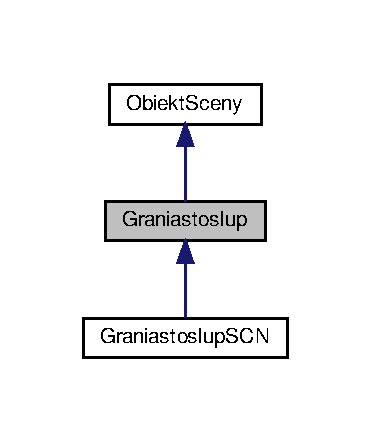
\includegraphics[width=178pt]{classGraniastoslup__inherit__graph}
\end{center}
\end{figure}


Diagram współpracy dla Graniastoslup\+:
\nopagebreak
\begin{figure}[H]
\begin{center}
\leavevmode
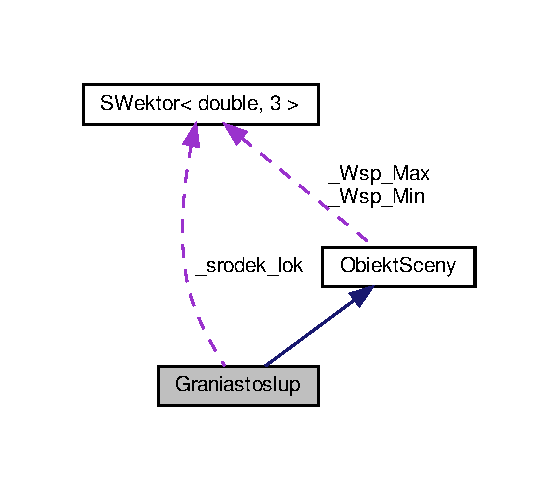
\includegraphics[width=268pt]{classGraniastoslup__coll__graph}
\end{center}
\end{figure}
\subsection*{Metody publiczne}
\begin{DoxyCompactItemize}
\item 
\hyperlink{classGraniastoslup_a1bc529dd6c0e18a1ae30ac5f7a0836e3}{Graniastoslup} ()
\begin{DoxyCompactList}\small\item\em Konstruktor bezparametryczny. \end{DoxyCompactList}\item 
void \hyperlink{classGraniastoslup_a348b25e965350ea5c8e5ebee39b35357}{Wyznacz\+\_\+\+Promien\+\_\+i\+\_\+\+Srodek} ()
\begin{DoxyCompactList}\small\item\em Metoda umozliwia okreslenie promienia i srodka. \end{DoxyCompactList}\item 
unsigned int const \hyperlink{classGraniastoslup_a7c5e6bb0c1761358af0e6ee80a8ab600}{Podaj\+Promien} () const
\begin{DoxyCompactList}\small\item\em Metoda umozliwia pobranie dlugosci promienia. \end{DoxyCompactList}\item 
\hyperlink{classSWektor}{Wektor3D} const \hyperlink{classGraniastoslup_aa573569ea9ca59cc99024c8e2a3d4308}{Podaj\+Srodek\+Lok} () const
\begin{DoxyCompactList}\small\item\em Metoda umozliwia pobranie wspolrzednych srodka. \end{DoxyCompactList}\item 
virtual bool \hyperlink{classGraniastoslup_a786313962b174b9c25084e45e827f39b}{Wyznacz\+Wsp} () override
\begin{DoxyCompactList}\small\item\em Metoda umozliwia wyznaczenie wspolrzednych skrajnych bryly. \end{DoxyCompactList}\end{DoxyCompactItemize}
\subsection*{Atrybuty prywatne}
\begin{DoxyCompactItemize}
\item 
unsigned int \hyperlink{classGraniastoslup_abaa6352f927e7317a0c02ec27b9a08a0}{\+\_\+promien}
\begin{DoxyCompactList}\small\item\em Pole przechowuje dlugosc promienia. \end{DoxyCompactList}\item 
\hyperlink{classSWektor}{Wektor3D} \hyperlink{classGraniastoslup_a8121bb2dc600bcbe9e852b3776f7df6f}{\+\_\+srodek\+\_\+lok}
\begin{DoxyCompactList}\small\item\em Pole przechowuje wspolrzedne srodka. \end{DoxyCompactList}\end{DoxyCompactItemize}


\subsection{Opis szczegółowy}
\hyperlink{classGraniastoslup}{Graniastoslup} jako bryla przestrzenna o promieniu i srodku lokalnym. 

Definicja klasy \hyperlink{classGraniastoslup}{Graniastoslup}, sluzacej do interpretacji zadanego obiektu jako graniastoslupa majacego okreslone wspolrzedne w ukladzie kartezjanskim. Ponadto obiekt zapamietuje wartosc swojego promienia oraz lokalne polozenie swojego srodka. 

\subsection{Dokumentacja konstruktora i destruktora}
\mbox{\Hypertarget{classGraniastoslup_a1bc529dd6c0e18a1ae30ac5f7a0836e3}\label{classGraniastoslup_a1bc529dd6c0e18a1ae30ac5f7a0836e3}} 
\index{Graniastoslup@{Graniastoslup}!Graniastoslup@{Graniastoslup}}
\index{Graniastoslup@{Graniastoslup}!Graniastoslup@{Graniastoslup}}
\subsubsection{\texorpdfstring{Graniastoslup()}{Graniastoslup()}}
{\footnotesize\ttfamily Graniastoslup\+::\+Graniastoslup (\begin{DoxyParamCaption}{ }\end{DoxyParamCaption})\hspace{0.3cm}{\ttfamily [inline]}}



Konstruktor bezparametryczny. 

Konstruktor bezparametryczny inicjalizujacy poczatkowa dlugosc promienia 

\subsection{Dokumentacja funkcji składowych}
\mbox{\Hypertarget{classGraniastoslup_a7c5e6bb0c1761358af0e6ee80a8ab600}\label{classGraniastoslup_a7c5e6bb0c1761358af0e6ee80a8ab600}} 
\index{Graniastoslup@{Graniastoslup}!Podaj\+Promien@{Podaj\+Promien}}
\index{Podaj\+Promien@{Podaj\+Promien}!Graniastoslup@{Graniastoslup}}
\subsubsection{\texorpdfstring{Podaj\+Promien()}{PodajPromien()}}
{\footnotesize\ttfamily unsigned int const Graniastoslup\+::\+Podaj\+Promien (\begin{DoxyParamCaption}{ }\end{DoxyParamCaption}) const\hspace{0.3cm}{\ttfamily [inline]}}



Metoda umozliwia pobranie dlugosci promienia. 

Metoda umozliwia pobranie wartosci promienia \begin{DoxyPrecond}{Warunek wstępny}
Wartosc promienia musi byc wczesniej wyliczona 
\end{DoxyPrecond}

\begin{DoxyRetVals}{Zwracane wartości}
{\em Wartosc} & {\itshape \+\_\+promien} \\
\hline
\end{DoxyRetVals}
\mbox{\Hypertarget{classGraniastoslup_aa573569ea9ca59cc99024c8e2a3d4308}\label{classGraniastoslup_aa573569ea9ca59cc99024c8e2a3d4308}} 
\index{Graniastoslup@{Graniastoslup}!Podaj\+Srodek\+Lok@{Podaj\+Srodek\+Lok}}
\index{Podaj\+Srodek\+Lok@{Podaj\+Srodek\+Lok}!Graniastoslup@{Graniastoslup}}
\subsubsection{\texorpdfstring{Podaj\+Srodek\+Lok()}{PodajSrodekLok()}}
{\footnotesize\ttfamily \hyperlink{classSWektor}{Wektor3D} const Graniastoslup\+::\+Podaj\+Srodek\+Lok (\begin{DoxyParamCaption}{ }\end{DoxyParamCaption}) const\hspace{0.3cm}{\ttfamily [inline]}}



Metoda umozliwia pobranie wspolrzednych srodka. 

Metoda umozliwia pobranie wartosci wspolrzednych srodka lokalnego bryly 
\begin{DoxyRetVals}{Zwracane wartości}
{\em Wektor3D} & {\itshape \+\_\+srodek\+\_\+lok} \\
\hline
\end{DoxyRetVals}
\mbox{\Hypertarget{classGraniastoslup_a348b25e965350ea5c8e5ebee39b35357}\label{classGraniastoslup_a348b25e965350ea5c8e5ebee39b35357}} 
\index{Graniastoslup@{Graniastoslup}!Wyznacz\+\_\+\+Promien\+\_\+i\+\_\+\+Srodek@{Wyznacz\+\_\+\+Promien\+\_\+i\+\_\+\+Srodek}}
\index{Wyznacz\+\_\+\+Promien\+\_\+i\+\_\+\+Srodek@{Wyznacz\+\_\+\+Promien\+\_\+i\+\_\+\+Srodek}!Graniastoslup@{Graniastoslup}}
\subsubsection{\texorpdfstring{Wyznacz\+\_\+\+Promien\+\_\+i\+\_\+\+Srodek()}{Wyznacz\_Promien\_i\_Srodek()}}
{\footnotesize\ttfamily void Graniastoslup\+::\+Wyznacz\+\_\+\+Promien\+\_\+i\+\_\+\+Srodek (\begin{DoxyParamCaption}{ }\end{DoxyParamCaption})}



Metoda umozliwia okreslenie promienia i srodka. 

Metoda umozliwia wyznaczenie wspolrzednych srodka lokalnego oraz dlugosci promienia bryly, a nastepnie zapamietanie ich wartosci w polach obiektu \begin{DoxyPrecond}{Warunek wstępny}
Wspolrzedne obiektu musza byc wczesniej poprawnie zapisane w pliku, ktorego nazwa zapisana jest przez pole {\itshape \+\_\+\+Plik\+\_\+\+Wsp\+\_\+\+Lokalne} 
\end{DoxyPrecond}
\mbox{\Hypertarget{classGraniastoslup_a786313962b174b9c25084e45e827f39b}\label{classGraniastoslup_a786313962b174b9c25084e45e827f39b}} 
\index{Graniastoslup@{Graniastoslup}!Wyznacz\+Wsp@{Wyznacz\+Wsp}}
\index{Wyznacz\+Wsp@{Wyznacz\+Wsp}!Graniastoslup@{Graniastoslup}}
\subsubsection{\texorpdfstring{Wyznacz\+Wsp()}{WyznaczWsp()}}
{\footnotesize\ttfamily bool Graniastoslup\+::\+Wyznacz\+Wsp (\begin{DoxyParamCaption}{ }\end{DoxyParamCaption})\hspace{0.3cm}{\ttfamily [override]}, {\ttfamily [virtual]}}



Metoda umozliwia wyznaczenie wspolrzednych skrajnych bryly. 

Metoda umozliwia wyznaczenie wspolrzednych skrajnych bryly, nadpisujac w odpowiedni sposob metode \hyperlink{classObiektSceny_a24dd0332c0755d7155128639a9a3e2b4}{Obiekt\+Sceny\+::\+Wyznacz\+Wsp()}

\begin{DoxyPrecond}{Warunek wstępny}
Obiekt musi miec poprawnie zadane nazwy plikow ze wspolrzednymi 
\end{DoxyPrecond}

\begin{DoxyRetVals}{Zwracane wartości}
{\em true} & -\/ proces przebiegł pomyślnie \\
\hline
{\em false} & -\/ nie udało sie wyznaczyc wspolrzednych skrajnych \\
\hline
\end{DoxyRetVals}


Implementuje \hyperlink{classObiektSceny_a24dd0332c0755d7155128639a9a3e2b4}{Obiekt\+Sceny}.



Reimplementowana w \hyperlink{classGraniastoslupSCN_a096492db05264adae9306f5fb50cc3c9}{Graniastoslup\+S\+CN}.



\subsection{Dokumentacja atrybutów składowych}
\mbox{\Hypertarget{classGraniastoslup_abaa6352f927e7317a0c02ec27b9a08a0}\label{classGraniastoslup_abaa6352f927e7317a0c02ec27b9a08a0}} 
\index{Graniastoslup@{Graniastoslup}!\+\_\+promien@{\+\_\+promien}}
\index{\+\_\+promien@{\+\_\+promien}!Graniastoslup@{Graniastoslup}}
\subsubsection{\texorpdfstring{\+\_\+promien}{\_promien}}
{\footnotesize\ttfamily unsigned int Graniastoslup\+::\+\_\+promien\hspace{0.3cm}{\ttfamily [private]}}



Pole przechowuje dlugosc promienia. 

Pole przechowuje dlugosc promienia bryly \mbox{\Hypertarget{classGraniastoslup_a8121bb2dc600bcbe9e852b3776f7df6f}\label{classGraniastoslup_a8121bb2dc600bcbe9e852b3776f7df6f}} 
\index{Graniastoslup@{Graniastoslup}!\+\_\+srodek\+\_\+lok@{\+\_\+srodek\+\_\+lok}}
\index{\+\_\+srodek\+\_\+lok@{\+\_\+srodek\+\_\+lok}!Graniastoslup@{Graniastoslup}}
\subsubsection{\texorpdfstring{\+\_\+srodek\+\_\+lok}{\_srodek\_lok}}
{\footnotesize\ttfamily \hyperlink{classSWektor}{Wektor3D} Graniastoslup\+::\+\_\+srodek\+\_\+lok\hspace{0.3cm}{\ttfamily [private]}}



Pole przechowuje wspolrzedne srodka. 

Pole przechowuje pierwotne wspolrzedne srodka bryly 

Dokumentacja dla tej klasy została wygenerowana z plików\+:\begin{DoxyCompactItemize}
\item 
inc/\hyperlink{Graniastoslup_8hh}{Graniastoslup.\+hh}\item 
src/\hyperlink{Graniastoslup_8cpp}{Graniastoslup.\+cpp}\end{DoxyCompactItemize}

\hypertarget{classGraniastoslupSCN}{}\section{Dokumentacja klasy Graniastoslup\+S\+CN}
\label{classGraniastoslupSCN}\index{Graniastoslup\+S\+CN@{Graniastoslup\+S\+CN}}


\hyperlink{classGraniastoslupSCN}{Graniastoslup\+S\+CN} jako \hyperlink{classGraniastoslup}{Graniastoslup} w ukladzie globalnym.  




{\ttfamily \#include $<$Graniastoslup\+S\+C\+N.\+hh$>$}



Diagram dziedziczenia dla Graniastoslup\+S\+CN
\nopagebreak
\begin{figure}[H]
\begin{center}
\leavevmode
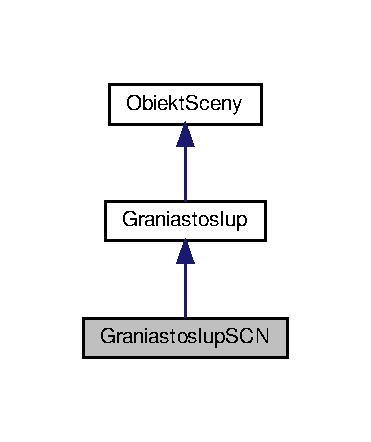
\includegraphics[width=178pt]{classGraniastoslupSCN__inherit__graph}
\end{center}
\end{figure}


Diagram współpracy dla Graniastoslup\+S\+CN\+:
\nopagebreak
\begin{figure}[H]
\begin{center}
\leavevmode
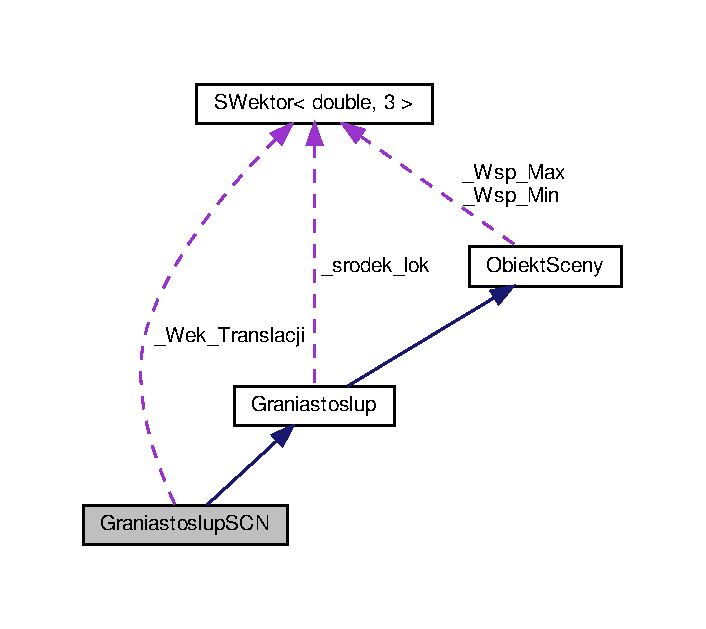
\includegraphics[width=339pt]{classGraniastoslupSCN__coll__graph}
\end{center}
\end{figure}
\subsection*{Metody publiczne}
\begin{DoxyCompactItemize}
\item 
\hyperlink{classGraniastoslupSCN_a1cf442360ec14fc7fa22af9ddefd1d35}{Graniastoslup\+S\+CN} ()
\begin{DoxyCompactList}\small\item\em Konstruktor obiektu \hyperlink{classGraniastoslupSCN}{Graniastoslup\+S\+CN}. \end{DoxyCompactList}\item 
void \hyperlink{classGraniastoslupSCN_a6c761ec9040c78b88e8f927bbe1fefb2}{Wybierz\+Plik\+Glob} (const char $\ast$Nazwa\+Pliku)
\begin{DoxyCompactList}\small\item\em Metoda umozliwia przypisanie obiektowi pliku ze wspolrzednymi globalnymi. \end{DoxyCompactList}\item 
const std\+::string \hyperlink{classGraniastoslupSCN_ad3d658eb048fd25af6a31a6416e02908}{Podaj\+Nazwe\+Pliku\+Glob} () const
\begin{DoxyCompactList}\small\item\em Metoda umozliwia pobranie nazwy przypisanego pliku ze wspolrzednymi globalnymi. \end{DoxyCompactList}\item 
virtual bool \hyperlink{classGraniastoslupSCN_a096492db05264adae9306f5fb50cc3c9}{Wyznacz\+Wsp} () override
\begin{DoxyCompactList}\small\item\em Metoda umozliwia wyznaczenie obecnych wspolrzednych skrajnych bryly. \end{DoxyCompactList}\item 
bool \hyperlink{classGraniastoslupSCN_a4bf899d8eba989560c5955748c2c5204}{Oblicz\+Globalne} () const
\begin{DoxyCompactList}\small\item\em Realizuje przeksztalcenie wspolrzednych lokalnych do ukladu globalnego. \end{DoxyCompactList}\item 
bool \hyperlink{classGraniastoslupSCN_a279b52ec2cb4c39f1025089695388a2a}{Wybierz\+Pliki} (const char $\ast$Nazwa\+Pliku\+We, const char $\ast$Nazwa\+Pliku\+Wy, unsigned int numer)
\begin{DoxyCompactList}\small\item\em Metoda umozliwia przypisanie obiektowi dwoch plikow. \end{DoxyCompactList}\item 
void \hyperlink{classGraniastoslupSCN_af074e119fe4e8a34d4be489d4d5512fe}{Zmien\+\_\+o\+\_\+kat} (int kat)
\begin{DoxyCompactList}\small\item\em Metoda umozliwia zmiane orientacji bryly wokol osi OZ. \end{DoxyCompactList}\item 
void \hyperlink{classGraniastoslupSCN_a66b1dda997b41aaa596ad6b953f06c8c}{Zmien\+\_\+o\+\_\+kat\+\_\+wlasny} (int kat)
\begin{DoxyCompactList}\small\item\em Metoda umozliwia zmiane orientacji bryly wokol osi OX. \end{DoxyCompactList}\item 
void \hyperlink{classGraniastoslupSCN_a65db4e5bc006a5969f5a2ebb8b2adaea}{Zmien\+\_\+o\+\_\+translacje} (\hyperlink{classSWektor}{Wektor3D} Translacja)
\begin{DoxyCompactList}\small\item\em Metoda umozliwia zmiane polozenia bryly. \end{DoxyCompactList}\item 
int const \hyperlink{classGraniastoslupSCN_a22fa17548fa2785b1c9850bb166fa1e7}{Podaj\+Kat\+Orientacji} () const
\begin{DoxyCompactList}\small\item\em Metoda umozliwia pobranie wartosci kata orientacji bryly. \end{DoxyCompactList}\item 
\hyperlink{classSWektor}{Wektor3D} const \hyperlink{classGraniastoslupSCN_a48c31869ef862c487bb511d8a121005b}{Podaj\+Polozenie} () const
\begin{DoxyCompactList}\small\item\em Metoda umozliwia pobranie wartosci wektora polozenia bryly. \end{DoxyCompactList}\end{DoxyCompactItemize}
\subsection*{Metody prywatne}
\begin{DoxyCompactItemize}
\item 
void \hyperlink{classGraniastoslupSCN_a848f8d3f0298dda442fab7acec295f80}{Zmien\+\_\+kat\+\_\+wlasny} ()
\begin{DoxyCompactList}\small\item\em Zmiana kata wlasnego, tj. \end{DoxyCompactList}\end{DoxyCompactItemize}
\subsection*{Atrybuty prywatne}
\begin{DoxyCompactItemize}
\item 
std\+::string \hyperlink{classGraniastoslupSCN_abd53a52e6fa9127c98d3922b4134fe67}{\+\_\+\+Plik\+\_\+\+Wsp\+\_\+\+Globalne}
\begin{DoxyCompactList}\small\item\em Pole przechowuje nazwe pliku z danymi globalnymi. \end{DoxyCompactList}\item 
int \hyperlink{classGraniastoslupSCN_a9fd5ceb4bf6119ef152db01d43d4925c}{\+\_\+\+Kat\+\_\+\+Orientacji\+\_\+\+OZ}
\begin{DoxyCompactList}\small\item\em Pole przechowuje miare kata orientacji\+OZ. \end{DoxyCompactList}\item 
int \hyperlink{classGraniastoslupSCN_a6c82bb652a2a7ebefc166864af4be36a}{\+\_\+\+Kat\+\_\+\+Orientacji\+\_\+\+OX}
\begin{DoxyCompactList}\small\item\em Pole przechowuje miare kata orientacji\+OX. \end{DoxyCompactList}\item 
\hyperlink{classSWektor}{Wektor3D} \hyperlink{classGraniastoslupSCN_a8d6e1399862324d18f3dee74c41212d0}{\+\_\+\+Wek\+\_\+\+Translacji}
\begin{DoxyCompactList}\small\item\em Pole przechowuje wektor translacji bryly. \end{DoxyCompactList}\end{DoxyCompactItemize}


\subsection{Opis szczegółowy}
\hyperlink{classGraniastoslupSCN}{Graniastoslup\+S\+CN} jako \hyperlink{classGraniastoslup}{Graniastoslup} w ukladzie globalnym. 

Definicja klasy \hyperlink{classGraniastoslupSCN}{Graniastoslup\+S\+CN}, sluzacej do interpretacji zadanego graniastoslupa jako obiektu rozbudowanego o mozliwosc okreslenia orientacji i przesuniecia w ukladzie globalnym 

\subsection{Dokumentacja konstruktora i destruktora}
\mbox{\Hypertarget{classGraniastoslupSCN_a1cf442360ec14fc7fa22af9ddefd1d35}\label{classGraniastoslupSCN_a1cf442360ec14fc7fa22af9ddefd1d35}} 
\index{Graniastoslup\+S\+CN@{Graniastoslup\+S\+CN}!Graniastoslup\+S\+CN@{Graniastoslup\+S\+CN}}
\index{Graniastoslup\+S\+CN@{Graniastoslup\+S\+CN}!Graniastoslup\+S\+CN@{Graniastoslup\+S\+CN}}
\subsubsection{\texorpdfstring{Graniastoslup\+S\+C\+N()}{GraniastoslupSCN()}}
{\footnotesize\ttfamily Graniastoslup\+S\+C\+N\+::\+Graniastoslup\+S\+CN (\begin{DoxyParamCaption}{ }\end{DoxyParamCaption})}



Konstruktor obiektu \hyperlink{classGraniastoslupSCN}{Graniastoslup\+S\+CN}. 

Konstruktor bezparametryczny obiektu \hyperlink{classGraniastoslupSCN}{Graniastoslup\+S\+CN}, ustawiajacy domyslna wartosc katow orientacji bryly na 0 

\subsection{Dokumentacja funkcji składowych}
\mbox{\Hypertarget{classGraniastoslupSCN_a4bf899d8eba989560c5955748c2c5204}\label{classGraniastoslupSCN_a4bf899d8eba989560c5955748c2c5204}} 
\index{Graniastoslup\+S\+CN@{Graniastoslup\+S\+CN}!Oblicz\+Globalne@{Oblicz\+Globalne}}
\index{Oblicz\+Globalne@{Oblicz\+Globalne}!Graniastoslup\+S\+CN@{Graniastoslup\+S\+CN}}
\subsubsection{\texorpdfstring{Oblicz\+Globalne()}{ObliczGlobalne()}}
{\footnotesize\ttfamily bool Graniastoslup\+S\+C\+N\+::\+Oblicz\+Globalne (\begin{DoxyParamCaption}{ }\end{DoxyParamCaption}) const}



Realizuje przeksztalcenie wspolrzednych lokalnych do ukladu globalnego. 

Realizuje przeksztalcenie wspolrzednych lokalnych do ukladu globalnego biorac pod uwage kat orientacji oraz wektor translacji bryly

\begin{DoxyPrecond}{Warunek wstępny}
Obiekt musi miec poprawnie zadane nazwy plikow ze wspolrzednymi 
\end{DoxyPrecond}

\begin{DoxyRetVals}{Zwracane wartości}
{\em true} & -\/ operacja przebiegla pomyslnie \\
\hline
{\em false} & -\/ nie udalo sie okreslic wspolrzednych globalnych -\/ blad prawidlowego odczytania wspolrzednych z pliku {\itshape \+\_\+\+Plik\+\_\+\+Wsp\+\_\+\+Lokalne} lub blad zapisu do pliku {\itshape \+\_\+\+Plik\+\_\+\+Wsp\+\_\+\+Globalne} \\
\hline
\end{DoxyRetVals}
\mbox{\Hypertarget{classGraniastoslupSCN_a22fa17548fa2785b1c9850bb166fa1e7}\label{classGraniastoslupSCN_a22fa17548fa2785b1c9850bb166fa1e7}} 
\index{Graniastoslup\+S\+CN@{Graniastoslup\+S\+CN}!Podaj\+Kat\+Orientacji@{Podaj\+Kat\+Orientacji}}
\index{Podaj\+Kat\+Orientacji@{Podaj\+Kat\+Orientacji}!Graniastoslup\+S\+CN@{Graniastoslup\+S\+CN}}
\subsubsection{\texorpdfstring{Podaj\+Kat\+Orientacji()}{PodajKatOrientacji()}}
{\footnotesize\ttfamily int const Graniastoslup\+S\+C\+N\+::\+Podaj\+Kat\+Orientacji (\begin{DoxyParamCaption}{ }\end{DoxyParamCaption}) const\hspace{0.3cm}{\ttfamily [inline]}}



Metoda umozliwia pobranie wartosci kata orientacji bryly. 

Metoda umozliwia pobranie wartosci okreslonego kata orientacji bryly 
\begin{DoxyRetVals}{Zwracane wartości}
{\em Wartosc} & {\itshape \+\_\+\+Kat\+\_\+\+Orientacji\+\_\+\+OZ} \\
\hline
\end{DoxyRetVals}
\mbox{\Hypertarget{classGraniastoslupSCN_ad3d658eb048fd25af6a31a6416e02908}\label{classGraniastoslupSCN_ad3d658eb048fd25af6a31a6416e02908}} 
\index{Graniastoslup\+S\+CN@{Graniastoslup\+S\+CN}!Podaj\+Nazwe\+Pliku\+Glob@{Podaj\+Nazwe\+Pliku\+Glob}}
\index{Podaj\+Nazwe\+Pliku\+Glob@{Podaj\+Nazwe\+Pliku\+Glob}!Graniastoslup\+S\+CN@{Graniastoslup\+S\+CN}}
\subsubsection{\texorpdfstring{Podaj\+Nazwe\+Pliku\+Glob()}{PodajNazwePlikuGlob()}}
{\footnotesize\ttfamily const std\+::string Graniastoslup\+S\+C\+N\+::\+Podaj\+Nazwe\+Pliku\+Glob (\begin{DoxyParamCaption}{ }\end{DoxyParamCaption}) const\hspace{0.3cm}{\ttfamily [inline]}}



Metoda umozliwia pobranie nazwy przypisanego pliku ze wspolrzednymi globalnymi. 

Metoda umozliwia pobranie nazwy przypisanego pliku, w ktorym beda znajdowac sie wyliczone wspolrzedne globalne obiektu \begin{DoxyPrecond}{Warunek wstępny}
Nazwa pliku ze wspolrzednymi globalnymi musi byc wczesniej okreslona 
\end{DoxyPrecond}

\begin{DoxyRetVals}{Zwracane wartości}
{\em Parametr} & {\itshape \+\_\+\+Plik\+\_\+\+Wsp\+\_\+\+Globalne} \\
\hline
\end{DoxyRetVals}
\mbox{\Hypertarget{classGraniastoslupSCN_a48c31869ef862c487bb511d8a121005b}\label{classGraniastoslupSCN_a48c31869ef862c487bb511d8a121005b}} 
\index{Graniastoslup\+S\+CN@{Graniastoslup\+S\+CN}!Podaj\+Polozenie@{Podaj\+Polozenie}}
\index{Podaj\+Polozenie@{Podaj\+Polozenie}!Graniastoslup\+S\+CN@{Graniastoslup\+S\+CN}}
\subsubsection{\texorpdfstring{Podaj\+Polozenie()}{PodajPolozenie()}}
{\footnotesize\ttfamily \hyperlink{classSWektor}{Wektor3D} const Graniastoslup\+S\+C\+N\+::\+Podaj\+Polozenie (\begin{DoxyParamCaption}{ }\end{DoxyParamCaption}) const\hspace{0.3cm}{\ttfamily [inline]}}



Metoda umozliwia pobranie wartosci wektora polozenia bryly. 

Metoda umozliwia pobranie wartosci okreslonego wektora polozenia bryly 
\begin{DoxyRetVals}{Zwracane wartości}
{\em Wektor3D} & {\itshape \+\_\+\+Wek\+\_\+\+Translacji} \\
\hline
\end{DoxyRetVals}
\mbox{\Hypertarget{classGraniastoslupSCN_a6c761ec9040c78b88e8f927bbe1fefb2}\label{classGraniastoslupSCN_a6c761ec9040c78b88e8f927bbe1fefb2}} 
\index{Graniastoslup\+S\+CN@{Graniastoslup\+S\+CN}!Wybierz\+Plik\+Glob@{Wybierz\+Plik\+Glob}}
\index{Wybierz\+Plik\+Glob@{Wybierz\+Plik\+Glob}!Graniastoslup\+S\+CN@{Graniastoslup\+S\+CN}}
\subsubsection{\texorpdfstring{Wybierz\+Plik\+Glob()}{WybierzPlikGlob()}}
{\footnotesize\ttfamily void Graniastoslup\+S\+C\+N\+::\+Wybierz\+Plik\+Glob (\begin{DoxyParamCaption}\item[{const char $\ast$}]{Nazwa\+Pliku }\end{DoxyParamCaption})\hspace{0.3cm}{\ttfamily [inline]}}



Metoda umozliwia przypisanie obiektowi pliku ze wspolrzednymi globalnymi. 

Metoda umozliwia przypisanie obiektowi pliku ze wspolrzednymi globalnymi


\begin{DoxyParams}[1]{Parametry}
\mbox{\tt in}  & {\em Nazwa\+Pliku} & -\/ Nazwa pliku ze wspolrzednymi globalnymi \\
\hline
\end{DoxyParams}
\mbox{\Hypertarget{classGraniastoslupSCN_a279b52ec2cb4c39f1025089695388a2a}\label{classGraniastoslupSCN_a279b52ec2cb4c39f1025089695388a2a}} 
\index{Graniastoslup\+S\+CN@{Graniastoslup\+S\+CN}!Wybierz\+Pliki@{Wybierz\+Pliki}}
\index{Wybierz\+Pliki@{Wybierz\+Pliki}!Graniastoslup\+S\+CN@{Graniastoslup\+S\+CN}}
\subsubsection{\texorpdfstring{Wybierz\+Pliki()}{WybierzPliki()}}
{\footnotesize\ttfamily bool Graniastoslup\+S\+C\+N\+::\+Wybierz\+Pliki (\begin{DoxyParamCaption}\item[{const char $\ast$}]{Nazwa\+Pliku\+We,  }\item[{const char $\ast$}]{Nazwa\+Pliku\+Wy,  }\item[{unsigned int}]{numer }\end{DoxyParamCaption})}



Metoda umozliwia przypisanie obiektowi dwoch plikow. 

Metoda umozliwia przypisanie obiektowi pliku ze wspolrzednymi poczatkowymi (lokalnymi) oraz pliku w ktorym zostana zapisane wspolrzedne przeksztalcone do ukladu globalnego (globalne). Wykorzystuje w tym celu metody \hyperlink{classObiektSceny_a84c19442a6a0757a1702e72effbb66d9}{Obiekt\+Sceny\+::\+Wybierz\+Plik\+Lok} \hyperlink{classGraniastoslupSCN_a6c761ec9040c78b88e8f927bbe1fefb2}{Graniastoslup\+S\+C\+N\+::\+Wybierz\+Plik\+Glob} \hyperlink{classGraniastoslupSCN_a4bf899d8eba989560c5955748c2c5204}{Graniastoslup\+S\+C\+N\+::\+Oblicz\+Globalne}


\begin{DoxyParams}[1]{Parametry}
\mbox{\tt in}  & {\em Nazwa\+Pliku\+We} & -\/ Nazwa pliku ze wspolrzednymi lokalnymi \\
\hline
\mbox{\tt in}  & {\em Nazwa\+Pliku\+Wy} & -\/ Nazwa pliku ze wspolrzednymi lokalnymi \\
\hline
\end{DoxyParams}

\begin{DoxyRetVals}{Zwracane wartości}
{\em true} & -\/ operacja przebiegla pomyslnie \\
\hline
{\em false} & -\/ metoda \hyperlink{classGraniastoslupSCN_a4bf899d8eba989560c5955748c2c5204}{Graniastoslup\+S\+C\+N\+::\+Oblicz\+Globalne} nie byla w stanie poprawnie wykonac operacji okreslenia i zapisania wspolrzednych globalnych \\
\hline
\end{DoxyRetVals}
\mbox{\Hypertarget{classGraniastoslupSCN_a096492db05264adae9306f5fb50cc3c9}\label{classGraniastoslupSCN_a096492db05264adae9306f5fb50cc3c9}} 
\index{Graniastoslup\+S\+CN@{Graniastoslup\+S\+CN}!Wyznacz\+Wsp@{Wyznacz\+Wsp}}
\index{Wyznacz\+Wsp@{Wyznacz\+Wsp}!Graniastoslup\+S\+CN@{Graniastoslup\+S\+CN}}
\subsubsection{\texorpdfstring{Wyznacz\+Wsp()}{WyznaczWsp()}}
{\footnotesize\ttfamily bool Graniastoslup\+S\+C\+N\+::\+Wyznacz\+Wsp (\begin{DoxyParamCaption}{ }\end{DoxyParamCaption})\hspace{0.3cm}{\ttfamily [override]}, {\ttfamily [virtual]}}



Metoda umozliwia wyznaczenie obecnych wspolrzednych skrajnych bryly. 

Metoda umozliwia wyznaczenie obecnych wspolrzednych skrajnych bryly, nadpisujac w odpowiedni sposob metode \hyperlink{classObiektSceny_a24dd0332c0755d7155128639a9a3e2b4}{Obiekt\+Sceny\+::\+Wyznacz\+Wsp()}

\begin{DoxyPrecond}{Warunek wstępny}
Obiekt musi miec poprawnie zadane nazwy plikow ze wspolrzednymi 
\end{DoxyPrecond}

\begin{DoxyRetVals}{Zwracane wartości}
{\em true} & -\/ proces przebiegł pomyślnie \\
\hline
{\em false} & -\/ nie udało sie wyznaczyc wspolrzednych skrajnych \\
\hline
\end{DoxyRetVals}


Reimplementowana z \hyperlink{classGraniastoslup_a786313962b174b9c25084e45e827f39b}{Graniastoslup}.

\mbox{\Hypertarget{classGraniastoslupSCN_a848f8d3f0298dda442fab7acec295f80}\label{classGraniastoslupSCN_a848f8d3f0298dda442fab7acec295f80}} 
\index{Graniastoslup\+S\+CN@{Graniastoslup\+S\+CN}!Zmien\+\_\+kat\+\_\+wlasny@{Zmien\+\_\+kat\+\_\+wlasny}}
\index{Zmien\+\_\+kat\+\_\+wlasny@{Zmien\+\_\+kat\+\_\+wlasny}!Graniastoslup\+S\+CN@{Graniastoslup\+S\+CN}}
\subsubsection{\texorpdfstring{Zmien\+\_\+kat\+\_\+wlasny()}{Zmien\_kat\_wlasny()}}
{\footnotesize\ttfamily void Graniastoslup\+S\+C\+N\+::\+Zmien\+\_\+kat\+\_\+wlasny (\begin{DoxyParamCaption}{ }\end{DoxyParamCaption})\hspace{0.3cm}{\ttfamily [inline]}, {\ttfamily [private]}}



Zmiana kata wlasnego, tj. 


\begin{DoxyParams}{Parametry}
{\em \+\_\+\+Kat\+\_\+\+Orientacji\+\_\+\+OX} & \\
\hline
\end{DoxyParams}
Metoda umozliwia obrot graniastoslupa wokol osi OX \mbox{\Hypertarget{classGraniastoslupSCN_af074e119fe4e8a34d4be489d4d5512fe}\label{classGraniastoslupSCN_af074e119fe4e8a34d4be489d4d5512fe}} 
\index{Graniastoslup\+S\+CN@{Graniastoslup\+S\+CN}!Zmien\+\_\+o\+\_\+kat@{Zmien\+\_\+o\+\_\+kat}}
\index{Zmien\+\_\+o\+\_\+kat@{Zmien\+\_\+o\+\_\+kat}!Graniastoslup\+S\+CN@{Graniastoslup\+S\+CN}}
\subsubsection{\texorpdfstring{Zmien\+\_\+o\+\_\+kat()}{Zmien\_o\_kat()}}
{\footnotesize\ttfamily void Graniastoslup\+S\+C\+N\+::\+Zmien\+\_\+o\+\_\+kat (\begin{DoxyParamCaption}\item[{int}]{kat }\end{DoxyParamCaption})}



Metoda umozliwia zmiane orientacji bryly wokol osi OZ. 

Metoda umozliwia zmiane kata orientacji bryly zapisanego w polu {\itshape \+\_\+\+Kat\+\_\+\+Orientacji\+\_\+\+OZ} zwiekszajac ja o wartosc zadana w parametrze {\itshape kat}. Jezeli wartosc kata orientacji wyniesie 360 lub -\/360, zostaje ona wyzerowana w celu zmniejszenia bledow dokladnosci obliczen


\begin{DoxyParams}[1]{Parametry}
\mbox{\tt in}  & {\em kat} & -\/ Kat o jaki zmieniona zostanie orientacja bryly \\
\hline
\end{DoxyParams}
\mbox{\Hypertarget{classGraniastoslupSCN_a66b1dda997b41aaa596ad6b953f06c8c}\label{classGraniastoslupSCN_a66b1dda997b41aaa596ad6b953f06c8c}} 
\index{Graniastoslup\+S\+CN@{Graniastoslup\+S\+CN}!Zmien\+\_\+o\+\_\+kat\+\_\+wlasny@{Zmien\+\_\+o\+\_\+kat\+\_\+wlasny}}
\index{Zmien\+\_\+o\+\_\+kat\+\_\+wlasny@{Zmien\+\_\+o\+\_\+kat\+\_\+wlasny}!Graniastoslup\+S\+CN@{Graniastoslup\+S\+CN}}
\subsubsection{\texorpdfstring{Zmien\+\_\+o\+\_\+kat\+\_\+wlasny()}{Zmien\_o\_kat\_wlasny()}}
{\footnotesize\ttfamily void Graniastoslup\+S\+C\+N\+::\+Zmien\+\_\+o\+\_\+kat\+\_\+wlasny (\begin{DoxyParamCaption}\item[{int}]{kat }\end{DoxyParamCaption})}



Metoda umozliwia zmiane orientacji bryly wokol osi OX. 

Metoda umozliwia zmiane kata orientacji bryly zapisanego w polu {\itshape \+\_\+\+Kat\+\_\+\+Orientacji\+\_\+\+OX} zwiekszajac ja o wartosc zadana w parametrze {\itshape kat}. Jezeli wartosc kata orientacji wyniesie 360 lub -\/360, zostaje ona wyzerowana w celu zmniejszenia bledow dokladnosci obliczen


\begin{DoxyParams}[1]{Parametry}
\mbox{\tt in}  & {\em kat} & -\/ Kat o jaki zmieniona zostanie orientacja bryly \\
\hline
\end{DoxyParams}
\mbox{\Hypertarget{classGraniastoslupSCN_a65db4e5bc006a5969f5a2ebb8b2adaea}\label{classGraniastoslupSCN_a65db4e5bc006a5969f5a2ebb8b2adaea}} 
\index{Graniastoslup\+S\+CN@{Graniastoslup\+S\+CN}!Zmien\+\_\+o\+\_\+translacje@{Zmien\+\_\+o\+\_\+translacje}}
\index{Zmien\+\_\+o\+\_\+translacje@{Zmien\+\_\+o\+\_\+translacje}!Graniastoslup\+S\+CN@{Graniastoslup\+S\+CN}}
\subsubsection{\texorpdfstring{Zmien\+\_\+o\+\_\+translacje()}{Zmien\_o\_translacje()}}
{\footnotesize\ttfamily void Graniastoslup\+S\+C\+N\+::\+Zmien\+\_\+o\+\_\+translacje (\begin{DoxyParamCaption}\item[{\hyperlink{classSWektor}{Wektor3D}}]{Translacja }\end{DoxyParamCaption})\hspace{0.3cm}{\ttfamily [inline]}}



Metoda umozliwia zmiane polozenia bryly. 

Metoda umozliwia zmiane wektora polozenia bryly zapisanego w polu {\itshape \+\_\+\+Wek\+\_\+\+Translacji} zwiekszajac ja o wektor zadany w parametrze {\itshape Translacja} 


\begin{DoxyParams}[1]{Parametry}
\mbox{\tt in}  & {\em Translacja} & -\/ Wektor o jaki zwiekszony zostanie wektor translacji bryly \\
\hline
\end{DoxyParams}


\subsection{Dokumentacja atrybutów składowych}
\mbox{\Hypertarget{classGraniastoslupSCN_a6c82bb652a2a7ebefc166864af4be36a}\label{classGraniastoslupSCN_a6c82bb652a2a7ebefc166864af4be36a}} 
\index{Graniastoslup\+S\+CN@{Graniastoslup\+S\+CN}!\+\_\+\+Kat\+\_\+\+Orientacji\+\_\+\+OX@{\+\_\+\+Kat\+\_\+\+Orientacji\+\_\+\+OX}}
\index{\+\_\+\+Kat\+\_\+\+Orientacji\+\_\+\+OX@{\+\_\+\+Kat\+\_\+\+Orientacji\+\_\+\+OX}!Graniastoslup\+S\+CN@{Graniastoslup\+S\+CN}}
\subsubsection{\texorpdfstring{\+\_\+\+Kat\+\_\+\+Orientacji\+\_\+\+OX}{\_Kat\_Orientacji\_OX}}
{\footnotesize\ttfamily int Graniastoslup\+S\+C\+N\+::\+\_\+\+Kat\+\_\+\+Orientacji\+\_\+\+OX\hspace{0.3cm}{\ttfamily [private]}}



Pole przechowuje miare kata orientacji\+OX. 

Pole przechowuje miare kata orientacji\+OX bryly okreslonego w stopniach \mbox{\Hypertarget{classGraniastoslupSCN_a9fd5ceb4bf6119ef152db01d43d4925c}\label{classGraniastoslupSCN_a9fd5ceb4bf6119ef152db01d43d4925c}} 
\index{Graniastoslup\+S\+CN@{Graniastoslup\+S\+CN}!\+\_\+\+Kat\+\_\+\+Orientacji\+\_\+\+OZ@{\+\_\+\+Kat\+\_\+\+Orientacji\+\_\+\+OZ}}
\index{\+\_\+\+Kat\+\_\+\+Orientacji\+\_\+\+OZ@{\+\_\+\+Kat\+\_\+\+Orientacji\+\_\+\+OZ}!Graniastoslup\+S\+CN@{Graniastoslup\+S\+CN}}
\subsubsection{\texorpdfstring{\+\_\+\+Kat\+\_\+\+Orientacji\+\_\+\+OZ}{\_Kat\_Orientacji\_OZ}}
{\footnotesize\ttfamily int Graniastoslup\+S\+C\+N\+::\+\_\+\+Kat\+\_\+\+Orientacji\+\_\+\+OZ\hspace{0.3cm}{\ttfamily [private]}}



Pole przechowuje miare kata orientacji\+OZ. 

Pole przechowuje miare kata orientacji\+OZ bryly okreslonego w stopniach \mbox{\Hypertarget{classGraniastoslupSCN_abd53a52e6fa9127c98d3922b4134fe67}\label{classGraniastoslupSCN_abd53a52e6fa9127c98d3922b4134fe67}} 
\index{Graniastoslup\+S\+CN@{Graniastoslup\+S\+CN}!\+\_\+\+Plik\+\_\+\+Wsp\+\_\+\+Globalne@{\+\_\+\+Plik\+\_\+\+Wsp\+\_\+\+Globalne}}
\index{\+\_\+\+Plik\+\_\+\+Wsp\+\_\+\+Globalne@{\+\_\+\+Plik\+\_\+\+Wsp\+\_\+\+Globalne}!Graniastoslup\+S\+CN@{Graniastoslup\+S\+CN}}
\subsubsection{\texorpdfstring{\+\_\+\+Plik\+\_\+\+Wsp\+\_\+\+Globalne}{\_Plik\_Wsp\_Globalne}}
{\footnotesize\ttfamily std\+::string Graniastoslup\+S\+C\+N\+::\+\_\+\+Plik\+\_\+\+Wsp\+\_\+\+Globalne\hspace{0.3cm}{\ttfamily [private]}}



Pole przechowuje nazwe pliku z danymi globalnymi. 

Pole przechowuje nazwe pliku z danymi globalnymi \mbox{\Hypertarget{classGraniastoslupSCN_a8d6e1399862324d18f3dee74c41212d0}\label{classGraniastoslupSCN_a8d6e1399862324d18f3dee74c41212d0}} 
\index{Graniastoslup\+S\+CN@{Graniastoslup\+S\+CN}!\+\_\+\+Wek\+\_\+\+Translacji@{\+\_\+\+Wek\+\_\+\+Translacji}}
\index{\+\_\+\+Wek\+\_\+\+Translacji@{\+\_\+\+Wek\+\_\+\+Translacji}!Graniastoslup\+S\+CN@{Graniastoslup\+S\+CN}}
\subsubsection{\texorpdfstring{\+\_\+\+Wek\+\_\+\+Translacji}{\_Wek\_Translacji}}
{\footnotesize\ttfamily \hyperlink{classSWektor}{Wektor3D} Graniastoslup\+S\+C\+N\+::\+\_\+\+Wek\+\_\+\+Translacji\hspace{0.3cm}{\ttfamily [private]}}



Pole przechowuje wektor translacji bryly. 

Pole przechowuje wektor translacji bryly -\/ domyslnie wektor zerowy 

Dokumentacja dla tej klasy została wygenerowana z plików\+:\begin{DoxyCompactItemize}
\item 
inc/\hyperlink{GraniastoslupSCN_8hh}{Graniastoslup\+S\+C\+N.\+hh}\item 
src/\hyperlink{GraniastoslupSCN_8cpp}{Graniastoslup\+S\+C\+N.\+cpp}\end{DoxyCompactItemize}

\hypertarget{classPzG_1_1InfoPlikuDoRysowania}{}\section{Dokumentacja klasy PzG\+:\+:Info\+Pliku\+Do\+Rysowania}
\label{classPzG_1_1InfoPlikuDoRysowania}\index{Pz\+G\+::\+Info\+Pliku\+Do\+Rysowania@{Pz\+G\+::\+Info\+Pliku\+Do\+Rysowania}}


Zestaw informacji dotyczący pliku i sposobu rysowania.  




{\ttfamily \#include $<$lacze\+\_\+do\+\_\+gnuplota.\+hh$>$}

\subsection*{Metody publiczne}
\begin{DoxyCompactItemize}
\item 
\hyperlink{classPzG_1_1InfoPlikuDoRysowania_a48bc8ad94ef5fd5120b668a566c9172e}{Info\+Pliku\+Do\+Rysowania} (const char $\ast$Nazwa\+Pliku, \hyperlink{namespacePzG_a705c92106f39b7d0c34a6739d10ff0b6}{Rodzaj\+Rysowania} Rodz\+Rys, int Szerokosc)
\item 
const std\+::string \hyperlink{classPzG_1_1InfoPlikuDoRysowania_ac92a5dc258f9b6164631e2ea5247a7a7}{Wez\+Nazwe\+Pliku} () const
\begin{DoxyCompactList}\small\item\em Udostępia nazwę pliku do rysowania. \end{DoxyCompactList}\item 
void \hyperlink{classPzG_1_1InfoPlikuDoRysowania_ae734c69f5cecf9c0584e3a7f433340ea}{Zmien\+Nazwe\+Pliku} (const std\+::string \&Nazwa\+Pliku)
\begin{DoxyCompactList}\small\item\em Zmienia nazwę pliku do rysowania. \end{DoxyCompactList}\item 
\hyperlink{namespacePzG_a705c92106f39b7d0c34a6739d10ff0b6}{Rodzaj\+Rysowania} \hyperlink{classPzG_1_1InfoPlikuDoRysowania_a6a46f3c7b7a08dfa9d694f387f873234}{Wez\+Rodz\+Rys} () const
\begin{DoxyCompactList}\small\item\em Udostępnia sposób rysowanej linii. \end{DoxyCompactList}\item 
int \hyperlink{classPzG_1_1InfoPlikuDoRysowania_a627bb615c50f3b03374774e6b974488b}{Wez\+Szerokosc} () const
\begin{DoxyCompactList}\small\item\em Udostępnia informację o szerokości linii. \end{DoxyCompactList}\end{DoxyCompactItemize}
\subsection*{Atrybuty prywatne}
\begin{DoxyCompactItemize}
\item 
std\+::string \hyperlink{classPzG_1_1InfoPlikuDoRysowania_a07ab06c56b9c3179e566a4123ab2a037}{\+\_\+\+Nazwa\+Pliku}
\begin{DoxyCompactList}\small\item\em Nazwa pliku z danymi do rysowania. \end{DoxyCompactList}\item 
int \hyperlink{classPzG_1_1InfoPlikuDoRysowania_a56a03dde7a7a414dbf3c230812a8d741}{\+\_\+\+Szerokosc}
\begin{DoxyCompactList}\small\item\em Szerokość użytego piórka. \end{DoxyCompactList}\item 
\hyperlink{namespacePzG_a705c92106f39b7d0c34a6739d10ff0b6}{Rodzaj\+Rysowania} \hyperlink{classPzG_1_1InfoPlikuDoRysowania_ac2512f2073c66164beb2e88db31344a4}{\+\_\+\+Rodz\+Rys}
\begin{DoxyCompactList}\small\item\em Sposób rysowania danej linii. \end{DoxyCompactList}\end{DoxyCompactItemize}


\subsection{Opis szczegółowy}
Zestaw informacji dotyczący pliku i sposobu rysowania. 

Klasa modeluje zestaw informacji dotyczący pliku i sposobu w jaki mają być wizualizowane zawarte w nim dane. 

\subsection{Dokumentacja konstruktora i destruktora}
\mbox{\Hypertarget{classPzG_1_1InfoPlikuDoRysowania_a48bc8ad94ef5fd5120b668a566c9172e}\label{classPzG_1_1InfoPlikuDoRysowania_a48bc8ad94ef5fd5120b668a566c9172e}} 
\index{Pz\+G\+::\+Info\+Pliku\+Do\+Rysowania@{Pz\+G\+::\+Info\+Pliku\+Do\+Rysowania}!Info\+Pliku\+Do\+Rysowania@{Info\+Pliku\+Do\+Rysowania}}
\index{Info\+Pliku\+Do\+Rysowania@{Info\+Pliku\+Do\+Rysowania}!Pz\+G\+::\+Info\+Pliku\+Do\+Rysowania@{Pz\+G\+::\+Info\+Pliku\+Do\+Rysowania}}
\subsubsection{\texorpdfstring{Info\+Pliku\+Do\+Rysowania()}{InfoPlikuDoRysowania()}}
{\footnotesize\ttfamily Pz\+G\+::\+Info\+Pliku\+Do\+Rysowania\+::\+Info\+Pliku\+Do\+Rysowania (\begin{DoxyParamCaption}\item[{const char $\ast$}]{Nazwa\+Pliku,  }\item[{\hyperlink{namespacePzG_a705c92106f39b7d0c34a6739d10ff0b6}{Rodzaj\+Rysowania}}]{Rodz\+Rys,  }\item[{int}]{Szerokosc }\end{DoxyParamCaption})\hspace{0.3cm}{\ttfamily [inline]}}

Inicjalizuje obiekt. 
\begin{DoxyParams}{Parametry}
{\em Nazwa\+Pliku} & -\/ nazwa pliku, z którego pobierane będą dane, \\
\hline
{\em Rodz\+Rys} & -\/ rodzaj rysowania linii, \\
\hline
{\em Szerokosc} & -\/ szerokosc linii. \\
\hline
\end{DoxyParams}


\subsection{Dokumentacja funkcji składowych}
\mbox{\Hypertarget{classPzG_1_1InfoPlikuDoRysowania_ac92a5dc258f9b6164631e2ea5247a7a7}\label{classPzG_1_1InfoPlikuDoRysowania_ac92a5dc258f9b6164631e2ea5247a7a7}} 
\index{Pz\+G\+::\+Info\+Pliku\+Do\+Rysowania@{Pz\+G\+::\+Info\+Pliku\+Do\+Rysowania}!Wez\+Nazwe\+Pliku@{Wez\+Nazwe\+Pliku}}
\index{Wez\+Nazwe\+Pliku@{Wez\+Nazwe\+Pliku}!Pz\+G\+::\+Info\+Pliku\+Do\+Rysowania@{Pz\+G\+::\+Info\+Pliku\+Do\+Rysowania}}
\subsubsection{\texorpdfstring{Wez\+Nazwe\+Pliku()}{WezNazwePliku()}}
{\footnotesize\ttfamily const std\+::string Pz\+G\+::\+Info\+Pliku\+Do\+Rysowania\+::\+Wez\+Nazwe\+Pliku (\begin{DoxyParamCaption}{ }\end{DoxyParamCaption}) const\hspace{0.3cm}{\ttfamily [inline]}}



Udostępia nazwę pliku do rysowania. 

Udostępnia nazwę pliku z danymi do rysowania. \mbox{\Hypertarget{classPzG_1_1InfoPlikuDoRysowania_a6a46f3c7b7a08dfa9d694f387f873234}\label{classPzG_1_1InfoPlikuDoRysowania_a6a46f3c7b7a08dfa9d694f387f873234}} 
\index{Pz\+G\+::\+Info\+Pliku\+Do\+Rysowania@{Pz\+G\+::\+Info\+Pliku\+Do\+Rysowania}!Wez\+Rodz\+Rys@{Wez\+Rodz\+Rys}}
\index{Wez\+Rodz\+Rys@{Wez\+Rodz\+Rys}!Pz\+G\+::\+Info\+Pliku\+Do\+Rysowania@{Pz\+G\+::\+Info\+Pliku\+Do\+Rysowania}}
\subsubsection{\texorpdfstring{Wez\+Rodz\+Rys()}{WezRodzRys()}}
{\footnotesize\ttfamily \hyperlink{namespacePzG_a705c92106f39b7d0c34a6739d10ff0b6}{Rodzaj\+Rysowania} Pz\+G\+::\+Info\+Pliku\+Do\+Rysowania\+::\+Wez\+Rodz\+Rys (\begin{DoxyParamCaption}{ }\end{DoxyParamCaption}) const\hspace{0.3cm}{\ttfamily [inline]}}



Udostępnia sposób rysowanej linii. 

Udostępnia informację o sposóbie rysowania linii. \mbox{\Hypertarget{classPzG_1_1InfoPlikuDoRysowania_a627bb615c50f3b03374774e6b974488b}\label{classPzG_1_1InfoPlikuDoRysowania_a627bb615c50f3b03374774e6b974488b}} 
\index{Pz\+G\+::\+Info\+Pliku\+Do\+Rysowania@{Pz\+G\+::\+Info\+Pliku\+Do\+Rysowania}!Wez\+Szerokosc@{Wez\+Szerokosc}}
\index{Wez\+Szerokosc@{Wez\+Szerokosc}!Pz\+G\+::\+Info\+Pliku\+Do\+Rysowania@{Pz\+G\+::\+Info\+Pliku\+Do\+Rysowania}}
\subsubsection{\texorpdfstring{Wez\+Szerokosc()}{WezSzerokosc()}}
{\footnotesize\ttfamily int Pz\+G\+::\+Info\+Pliku\+Do\+Rysowania\+::\+Wez\+Szerokosc (\begin{DoxyParamCaption}{ }\end{DoxyParamCaption}) const\hspace{0.3cm}{\ttfamily [inline]}}



Udostępnia informację o szerokości linii. 

Udostępnia informację o szerokości rysowanej linii. \mbox{\Hypertarget{classPzG_1_1InfoPlikuDoRysowania_ae734c69f5cecf9c0584e3a7f433340ea}\label{classPzG_1_1InfoPlikuDoRysowania_ae734c69f5cecf9c0584e3a7f433340ea}} 
\index{Pz\+G\+::\+Info\+Pliku\+Do\+Rysowania@{Pz\+G\+::\+Info\+Pliku\+Do\+Rysowania}!Zmien\+Nazwe\+Pliku@{Zmien\+Nazwe\+Pliku}}
\index{Zmien\+Nazwe\+Pliku@{Zmien\+Nazwe\+Pliku}!Pz\+G\+::\+Info\+Pliku\+Do\+Rysowania@{Pz\+G\+::\+Info\+Pliku\+Do\+Rysowania}}
\subsubsection{\texorpdfstring{Zmien\+Nazwe\+Pliku()}{ZmienNazwePliku()}}
{\footnotesize\ttfamily void Pz\+G\+::\+Info\+Pliku\+Do\+Rysowania\+::\+Zmien\+Nazwe\+Pliku (\begin{DoxyParamCaption}\item[{const std\+::string \&}]{Nazwa\+Pliku }\end{DoxyParamCaption})\hspace{0.3cm}{\ttfamily [inline]}}



Zmienia nazwę pliku do rysowania. 

Zmienia nazwę pliku z danymi do rysowania. 

\subsection{Dokumentacja atrybutów składowych}
\mbox{\Hypertarget{classPzG_1_1InfoPlikuDoRysowania_a07ab06c56b9c3179e566a4123ab2a037}\label{classPzG_1_1InfoPlikuDoRysowania_a07ab06c56b9c3179e566a4123ab2a037}} 
\index{Pz\+G\+::\+Info\+Pliku\+Do\+Rysowania@{Pz\+G\+::\+Info\+Pliku\+Do\+Rysowania}!\+\_\+\+Nazwa\+Pliku@{\+\_\+\+Nazwa\+Pliku}}
\index{\+\_\+\+Nazwa\+Pliku@{\+\_\+\+Nazwa\+Pliku}!Pz\+G\+::\+Info\+Pliku\+Do\+Rysowania@{Pz\+G\+::\+Info\+Pliku\+Do\+Rysowania}}
\subsubsection{\texorpdfstring{\+\_\+\+Nazwa\+Pliku}{\_NazwaPliku}}
{\footnotesize\ttfamily std\+::string Pz\+G\+::\+Info\+Pliku\+Do\+Rysowania\+::\+\_\+\+Nazwa\+Pliku\hspace{0.3cm}{\ttfamily [private]}}



Nazwa pliku z danymi do rysowania. 

Nazwa pliku z danymi do rysowania. \mbox{\Hypertarget{classPzG_1_1InfoPlikuDoRysowania_ac2512f2073c66164beb2e88db31344a4}\label{classPzG_1_1InfoPlikuDoRysowania_ac2512f2073c66164beb2e88db31344a4}} 
\index{Pz\+G\+::\+Info\+Pliku\+Do\+Rysowania@{Pz\+G\+::\+Info\+Pliku\+Do\+Rysowania}!\+\_\+\+Rodz\+Rys@{\+\_\+\+Rodz\+Rys}}
\index{\+\_\+\+Rodz\+Rys@{\+\_\+\+Rodz\+Rys}!Pz\+G\+::\+Info\+Pliku\+Do\+Rysowania@{Pz\+G\+::\+Info\+Pliku\+Do\+Rysowania}}
\subsubsection{\texorpdfstring{\+\_\+\+Rodz\+Rys}{\_RodzRys}}
{\footnotesize\ttfamily \hyperlink{namespacePzG_a705c92106f39b7d0c34a6739d10ff0b6}{Rodzaj\+Rysowania} Pz\+G\+::\+Info\+Pliku\+Do\+Rysowania\+::\+\_\+\+Rodz\+Rys\hspace{0.3cm}{\ttfamily [private]}}



Sposób rysowania danej linii. 

Przechowuje informacje o sposobie rysowania linii. \mbox{\Hypertarget{classPzG_1_1InfoPlikuDoRysowania_a56a03dde7a7a414dbf3c230812a8d741}\label{classPzG_1_1InfoPlikuDoRysowania_a56a03dde7a7a414dbf3c230812a8d741}} 
\index{Pz\+G\+::\+Info\+Pliku\+Do\+Rysowania@{Pz\+G\+::\+Info\+Pliku\+Do\+Rysowania}!\+\_\+\+Szerokosc@{\+\_\+\+Szerokosc}}
\index{\+\_\+\+Szerokosc@{\+\_\+\+Szerokosc}!Pz\+G\+::\+Info\+Pliku\+Do\+Rysowania@{Pz\+G\+::\+Info\+Pliku\+Do\+Rysowania}}
\subsubsection{\texorpdfstring{\+\_\+\+Szerokosc}{\_Szerokosc}}
{\footnotesize\ttfamily int Pz\+G\+::\+Info\+Pliku\+Do\+Rysowania\+::\+\_\+\+Szerokosc\hspace{0.3cm}{\ttfamily [private]}}



Szerokość użytego piórka. 

Określa szerokość piórka, jakie ma być użyte do rysowania obiektów graficznych. 

Dokumentacja dla tej klasy została wygenerowana z pliku\+:\begin{DoxyCompactItemize}
\item 
inc/\hyperlink{lacze__do__gnuplota_8hh}{lacze\+\_\+do\+\_\+gnuplota.\+hh}\end{DoxyCompactItemize}

\hypertarget{classPzG_1_1LaczeDoGNUPlota}{}\section{Dokumentacja klasy PzG\+:\+:Lacze\+Do\+G\+N\+U\+Plota}
\label{classPzG_1_1LaczeDoGNUPlota}\index{Pz\+G\+::\+Lacze\+Do\+G\+N\+U\+Plota@{Pz\+G\+::\+Lacze\+Do\+G\+N\+U\+Plota}}


Klasa realizuje interfejs do programu G\+N\+U\+Plot.  




{\ttfamily \#include $<$lacze\+\_\+do\+\_\+gnuplota.\+hh$>$}

\subsection*{Metody publiczne}
\begin{DoxyCompactItemize}
\item 
void \hyperlink{classPzG_1_1LaczeDoGNUPlota_a11421d7c67deab6b7524cc492407e897}{Pokaz\+Os\+\_\+\+OX} (bool Pokaz)
\begin{DoxyCompactList}\small\item\em Umożliwia lub zabrania rysowania osi OX. \end{DoxyCompactList}\item 
bool \hyperlink{classPzG_1_1LaczeDoGNUPlota_ae112972af57167c3b053bf922bce6bbf}{Pokaz\+Os\+\_\+\+OX} () const
\begin{DoxyCompactList}\small\item\em Czy oś OX ma być rysowana. \end{DoxyCompactList}\item 
void \hyperlink{classPzG_1_1LaczeDoGNUPlota_a7c3db909b266fc30808e86406c04b516}{Pokaz\+Os\+\_\+\+OY} (bool Pokaz)
\begin{DoxyCompactList}\small\item\em Umożliwia lub zabrania rysowania osi OY. \end{DoxyCompactList}\item 
bool \hyperlink{classPzG_1_1LaczeDoGNUPlota_a7298f469f6932f5c808dcf620650b4b8}{Pokaz\+Os\+\_\+\+OY} () const
\begin{DoxyCompactList}\small\item\em Czy oś OY ma być rysowana. \end{DoxyCompactList}\item 
void \hyperlink{classPzG_1_1LaczeDoGNUPlota_a9fabfe88cb1801a5de8923f45f514b99}{Pokaz\+Os\+\_\+\+OZ} (bool Pokaz)
\begin{DoxyCompactList}\small\item\em Umożliwia lub zabrania rysowania osi OZ. \end{DoxyCompactList}\item 
bool \hyperlink{classPzG_1_1LaczeDoGNUPlota_a22c708af33c57bf3b5d1b4e82b4017b7}{Pokaz\+Os\+\_\+\+OZ} () const
\begin{DoxyCompactList}\small\item\em Czy oś OZ ma być rysowana. \end{DoxyCompactList}\item 
float \hyperlink{classPzG_1_1LaczeDoGNUPlota_a66836c9749bf179420e4ca3e9447efd7}{Xmin} () const
\item 
float \hyperlink{classPzG_1_1LaczeDoGNUPlota_a8e23479629af3df3d352b7839ae396b8}{Xmax} () const
\item 
float \hyperlink{classPzG_1_1LaczeDoGNUPlota_a9352c0382bfaeaaba9f65399a7383164}{Ymin} () const
\item 
float \hyperlink{classPzG_1_1LaczeDoGNUPlota_ac54e4e7448ce3bd324efdc94a999f535}{Ymax} () const
\item 
float \hyperlink{classPzG_1_1LaczeDoGNUPlota_a9068bd9a9873ba9c6d70016f1ae7cd7f}{Zmin} () const
\item 
float \hyperlink{classPzG_1_1LaczeDoGNUPlota_a20a5d03e1fc19c682032bffc54340f12}{Zmax} () const
\item 
void \hyperlink{classPzG_1_1LaczeDoGNUPlota_a10950349b348fd3a3d4143e95337527c}{Zmien\+Tryb\+Rys} (\hyperlink{namespacePzG_aeedae1ef10c66d720f9e89de408ca4ca}{Tryb\+Rysowania} Tryb)
\begin{DoxyCompactList}\small\item\em Zmienia tryb rysowania. \end{DoxyCompactList}\item 
\hyperlink{namespacePzG_aeedae1ef10c66d720f9e89de408ca4ca}{Tryb\+Rysowania} \hyperlink{classPzG_1_1LaczeDoGNUPlota_a7c417f27b4b112f58a5be3ce6ea8d1fe}{Wez\+Tryb\+Rys} () const
\begin{DoxyCompactList}\small\item\em Udostępnia aktualny tryb rysowania. \end{DoxyCompactList}\item 
void \hyperlink{classPzG_1_1LaczeDoGNUPlota_a9c91987dfc869d6fcea96205c581daef}{Ustaw\+ZakresX} (float Xo, float Xn)
\begin{DoxyCompactList}\small\item\em Ustawia zakres osi {\itshape OX}. \end{DoxyCompactList}\item 
void \hyperlink{classPzG_1_1LaczeDoGNUPlota_a54c6e9cf9ab2eae479451fd953c2717c}{Ustaw\+ZakresY} (float Yo, float Yn)
\begin{DoxyCompactList}\small\item\em Ustawia zakres osi {\itshape OY}. \end{DoxyCompactList}\item 
void \hyperlink{classPzG_1_1LaczeDoGNUPlota_a1dbbb2b86fb13b8632e6bad9df2a82e3}{Ustaw\+ZakresZ} (float Zo, float Zn)
\begin{DoxyCompactList}\small\item\em Ustawia zakres osi {\itshape OZ}. \end{DoxyCompactList}\item 
float \hyperlink{classPzG_1_1LaczeDoGNUPlota_a4b1eb252fd785a5aeff938e7b2dce2b1}{SkalaX} () const
\begin{DoxyCompactList}\small\item\em Udostępnia skalę dla osi {\itshape OX}. \end{DoxyCompactList}\item 
float \hyperlink{classPzG_1_1LaczeDoGNUPlota_a44f922ccbc508d6cd7809c669238dae3}{SkalaZ} () const
\begin{DoxyCompactList}\small\item\em Udostępnia skalę dla osi {\itshape OZ}. \end{DoxyCompactList}\item 
void \hyperlink{classPzG_1_1LaczeDoGNUPlota_a855b8338bfe3e5d294d719f24b11090e}{Ustaw\+SkaleX} (float skala\+\_\+x)
\begin{DoxyCompactList}\small\item\em Zadaje skalę wzdłuż osi {\itshape OZ}. \end{DoxyCompactList}\item 
void \hyperlink{classPzG_1_1LaczeDoGNUPlota_ab0486db3166d8db6580a221079af241f}{Ustaw\+SkaleZ} (float skala\+\_\+z)
\begin{DoxyCompactList}\small\item\em Zadaje skalę wzdłuż osi {\itshape OZ}. \end{DoxyCompactList}\item 
void \hyperlink{classPzG_1_1LaczeDoGNUPlota_a4308151b54e105d302803146a3238699}{Ustaw\+Skale\+XZ} (float skala\+\_\+x, float skala\+\_\+z)
\begin{DoxyCompactList}\small\item\em Zadaje skalę wzdłuż osi {\itshape OX} i {\itshape OZ}. \end{DoxyCompactList}\item 
float \hyperlink{classPzG_1_1LaczeDoGNUPlota_addf0b844f626f3f5220de70efcbbdbb3}{RotacjaX} () const
\item 
float \hyperlink{classPzG_1_1LaczeDoGNUPlota_a9dac73754fab10644b287756003e9c79}{RotacjaZ} () const
\item 
void \hyperlink{classPzG_1_1LaczeDoGNUPlota_a88324c53a70846fb6bc9d918ce21fd56}{Ustaw\+RotacjeX} (float kat\+\_\+x)
\begin{DoxyCompactList}\small\item\em Ustawia rotację wokół osi {\itshape OX}. \end{DoxyCompactList}\item 
void \hyperlink{classPzG_1_1LaczeDoGNUPlota_a458399aa2a8f4b3f00ccd5b272857ea1}{Ustaw\+RotacjeZ} (float kat\+\_\+z)
\begin{DoxyCompactList}\small\item\em Ustawia rotację wokół osi {\itshape OZ}. \end{DoxyCompactList}\item 
void \hyperlink{classPzG_1_1LaczeDoGNUPlota_a94d8527fd78048ed6cb32ffb29e5f903}{Ustaw\+Rotacje\+XZ} (float kat\+\_\+x, float kat\+\_\+z)
\begin{DoxyCompactList}\small\item\em Ustawia rotację wokół osi {\itshape OX} i {\itshape OZ}. \end{DoxyCompactList}\item 
void \hyperlink{classPzG_1_1LaczeDoGNUPlota_a4531e6d166faf2e2c8bb4a54a9c9e1f8}{Wyswietlaj\+Komunikaty\+Bledow} (bool Tryb=true)
\begin{DoxyCompactList}\small\item\em Zezwala lub zabrania wyświetlania komunikatów. \end{DoxyCompactList}\item 
bool \hyperlink{classPzG_1_1LaczeDoGNUPlota_a34bd48f57c0fd69c12bf4127a1cacd8f}{Dodaj\+Nazwe\+Pliku} (const char $\ast$Nazwa\+Pliku, \hyperlink{namespacePzG_a705c92106f39b7d0c34a6739d10ff0b6}{Rodzaj\+Rysowania} Rodz\+Rys=R\+R\+\_\+\+Ciagly, int Szerokosc=1)
\begin{DoxyCompactList}\small\item\em Dodaje nazwę pliku. \end{DoxyCompactList}\item 
bool \hyperlink{classPzG_1_1LaczeDoGNUPlota_ad3d7607946b82aa941d786dcd086d27e}{Dopisz\+Rysowanie\+Z\+Plikow} (std\+::string \&Polecenie, char const $\ast$$\ast$Sep)
\begin{DoxyCompactList}\small\item\em Tworzy listę parametrów umożliwiających rysowanie brył z plików. \end{DoxyCompactList}\item 
bool \hyperlink{classPzG_1_1LaczeDoGNUPlota_af8be8aeb3b1b524fab67d4411cba5b9e}{Czy\+Polaczenie\+Jest\+Zainicjowane} () const
\begin{DoxyCompactList}\small\item\em Informuje, czy połączenie z {\itshape gnuplot\textquotesingle{}em} jest zainicjalizowane. \end{DoxyCompactList}\item 
bool \hyperlink{classPzG_1_1LaczeDoGNUPlota_a065f5b8402737cc62b0ad4f66d028335}{Rysuj} ()
\item 
bool \hyperlink{classPzG_1_1LaczeDoGNUPlota_addae9ac156ae2fb227f792faff3aa148}{Rysuj\+Do\+Pliku} (const char $\ast$Nazwa\+Pliku)
\item 
bool \hyperlink{classPzG_1_1LaczeDoGNUPlota_a200ce6bdb980c314a9eafe49e8f2dd5e}{Inicjalizuj} ()
\begin{DoxyCompactList}\small\item\em Inicjalizuje połączenie z programem {\itshape gnuplot}. \end{DoxyCompactList}\item 
void \hyperlink{classPzG_1_1LaczeDoGNUPlota_a75f599f17413ea8602c6dbba09f36407}{Usun\+Ostatnia\+Nazwe} ()
\begin{DoxyCompactList}\small\item\em Usuwa ostatnią nazwę pliku. \end{DoxyCompactList}\item 
void \hyperlink{classPzG_1_1LaczeDoGNUPlota_a89a1d90d017d264cd26398464d074073}{Usun\+Wszystkie\+Nazwy\+Plikow} ()
\begin{DoxyCompactList}\small\item\em Kasuje zawartość listy nazw plików. \end{DoxyCompactList}\end{DoxyCompactItemize}
\subsection*{Metody chronione}
\begin{DoxyCompactItemize}
\item 
virtual bool \hyperlink{classPzG_1_1LaczeDoGNUPlota_a25585ec3f1bd3b6bf42f374c38b8d237}{Dopisz\+Pliki\+Do\+Polecenia\+Rysowania} (std\+::string \&Polecenie, char const $\ast$$\ast$Sep)
\begin{DoxyCompactList}\small\item\em Tworzy listę parametrów umożliwiających rysowanie dodatkowych elementów. \end{DoxyCompactList}\item 
std\+::string \hyperlink{classPzG_1_1LaczeDoGNUPlota_a4579aecf7b4777fdde0cae4e98c275c2}{Zapisz\+Ustawienie\+Zakresu} (char Os) const
\begin{DoxyCompactList}\small\item\em Tworzy polecenie ustawiające zakres dla danej współrzędnej. \end{DoxyCompactList}\item 
std\+::string \hyperlink{classPzG_1_1LaczeDoGNUPlota_aa92b463e8cbae31b50dd797a4183bce8}{Zapisz\+Ustawienie\+Rotacji\+I\+Skali} () const
\begin{DoxyCompactList}\small\item\em Tworzy polecenie ustawiające punkt obserwacji. \end{DoxyCompactList}\item 
bool \hyperlink{classPzG_1_1LaczeDoGNUPlota_a5063854b7232a7951d120a21df63f2b7}{Przeslij\+Do\+G\+N\+U\+Plota} (const char $\ast$Polecenie)
\item 
bool \hyperlink{classPzG_1_1LaczeDoGNUPlota_a5e4f3a226ed36f7110032d802d84847c}{Czy\+Wyswietlac\+Komunikaty} () const
\begin{DoxyCompactList}\small\item\em Udostępnia informację czy mają być wyświetlane informacje o błędach. \end{DoxyCompactList}\item 
bool \hyperlink{classPzG_1_1LaczeDoGNUPlota_a1c7b9acc40de8d8bbb40fb0722512933}{Utworz\+Proces\+Potomny} ()
\begin{DoxyCompactList}\small\item\em Uruchamia program {\itshape gnuplot} jako proces potomny. \end{DoxyCompactList}\item 
void \hyperlink{classPzG_1_1LaczeDoGNUPlota_a90056743aeaa546721528005f2cf41e6}{Komunikat\+Bledu} (const char $\ast$Komunikat) const
\item 
void \hyperlink{classPzG_1_1LaczeDoGNUPlota_a0da98f68f533070d5a32adbdb519cf56}{Buduj\+Preambule\+Polecenia\+Rysowania} (std\+::string \&Preambula) const
\begin{DoxyCompactList}\small\item\em Tworzy preambułę poprzedzającą polecenie rysowania. \end{DoxyCompactList}\item 
void \hyperlink{classPzG_1_1LaczeDoGNUPlota_a0ac655ff1934abb69ea668cd92ae77ec}{Buduj\+Preambule\+\_\+2D} (std\+::string \&Preambula) const
\begin{DoxyCompactList}\small\item\em Tworzy preambułę poprzedzającą polecenie rysowania w trybie 2D. \end{DoxyCompactList}\item 
void \hyperlink{classPzG_1_1LaczeDoGNUPlota_a50a544677e52829cac4dd4a95b821dcb}{Buduj\+Preambule\+\_\+3D} (std\+::string \&Preambula) const
\begin{DoxyCompactList}\small\item\em Tworzy preambułę poprzedzającą polecenie rysowania w trybie 3D. \end{DoxyCompactList}\end{DoxyCompactItemize}
\subsection*{Atrybuty chronione}
\begin{DoxyCompactItemize}
\item 
int \hyperlink{classPzG_1_1LaczeDoGNUPlota_adc3a2250216c2473a61da379da70b2d7}{\+\_\+\+Wejscie\+\_\+\+G\+N\+U\+Plota}
\item 
int \hyperlink{classPzG_1_1LaczeDoGNUPlota_a7d05a4767a35ee494d59724bb740dbc2}{\+\_\+\+Wyjscie\+\_\+\+G\+N\+U\+Plota}
\item 
bool \hyperlink{classPzG_1_1LaczeDoGNUPlota_a2f2800f14ebfe1caef0b4d30c410a7fe}{\+\_\+\+Wyswietlaj\+Komunikaty\+O\+Bledach}
\begin{DoxyCompactList}\small\item\em Decyduje czy mają być wyświetlane komunikaty o błędach, czy też nie. \end{DoxyCompactList}\item 
\hyperlink{namespacePzG_aeedae1ef10c66d720f9e89de408ca4ca}{Tryb\+Rysowania} \hyperlink{classPzG_1_1LaczeDoGNUPlota_a00e3a51bb47d3fb26eee875dc48215db}{\+\_\+\+Tryb\+Rys}
\begin{DoxyCompactList}\small\item\em Określa aktualny tryb rysowania. \end{DoxyCompactList}\item 
float \hyperlink{classPzG_1_1LaczeDoGNUPlota_a69d530edfe769e38448972e897456deb}{\+\_\+\+Xmin}
\begin{DoxyCompactList}\small\item\em Dolny zakres wyświetlanej skali skali dla osi {\itshape OX}. \end{DoxyCompactList}\item 
float \hyperlink{classPzG_1_1LaczeDoGNUPlota_a847e00678a413ab076ccbcb7eba3ae58}{\+\_\+\+Xmax}
\begin{DoxyCompactList}\small\item\em Górny zakres wyświetlanej skali skali dla osi {\itshape OX}. \end{DoxyCompactList}\item 
float \hyperlink{classPzG_1_1LaczeDoGNUPlota_abc555fd6b82b0d5c9efb4802b58dc317}{\+\_\+\+Ymin}
\begin{DoxyCompactList}\small\item\em Dolny zakres wyświetlanej skali skali dla osi {\itshape OY}. \end{DoxyCompactList}\item 
float \hyperlink{classPzG_1_1LaczeDoGNUPlota_ad7dfd3fad82ea0720ec89eacc18410bf}{\+\_\+\+Ymax}
\begin{DoxyCompactList}\small\item\em Górny zakres wyświetlanej skali skali dla osi {\itshape OY}. \end{DoxyCompactList}\item 
float \hyperlink{classPzG_1_1LaczeDoGNUPlota_a8f9797e881df35f4206cb7d8030e5edc}{\+\_\+\+Zmin}
\begin{DoxyCompactList}\small\item\em Dolny zakres wyświetlanej skali skali dla osi {\itshape OZ}. \end{DoxyCompactList}\item 
float \hyperlink{classPzG_1_1LaczeDoGNUPlota_a26949eedd421832f0f206ce3c8f90694}{\+\_\+\+Zmax}
\begin{DoxyCompactList}\small\item\em Górny zakres wyświetlanej skali skali dla osi {\itshape OZ}. \end{DoxyCompactList}\item 
float \hyperlink{classPzG_1_1LaczeDoGNUPlota_a2c9303c4dbb4c9f0ddc4f1fe02eb3f70}{\+\_\+\+Xskala}
\item 
float \hyperlink{classPzG_1_1LaczeDoGNUPlota_a85446d06b2d714b2f852ef43c47c73c1}{\+\_\+\+Zskala}
\item 
float \hyperlink{classPzG_1_1LaczeDoGNUPlota_a21e77f0a2bfb7fed989b6dc2d64b5a7e}{\+\_\+\+Xrotacja}
\item 
float \hyperlink{classPzG_1_1LaczeDoGNUPlota_aa65781b1ff96dfb31a780e98ee28d6ed}{\+\_\+\+Zrotacja}
\item 
bool \hyperlink{classPzG_1_1LaczeDoGNUPlota_a833aa8994b9913786f920ec8c259731f}{\+\_\+\+Pokaz\+Os\+\_\+\+OX}
\begin{DoxyCompactList}\small\item\em Czy oś OX ma być widoczna. \end{DoxyCompactList}\item 
bool \hyperlink{classPzG_1_1LaczeDoGNUPlota_ae8d9b4dac5eae6ce86b7043c45b70ed8}{\+\_\+\+Pokaz\+Os\+\_\+\+OY}
\begin{DoxyCompactList}\small\item\em Czy oś OY ma być widoczna. \end{DoxyCompactList}\item 
bool \hyperlink{classPzG_1_1LaczeDoGNUPlota_a5b0afc06dc248790d2e7475b2162e309}{\+\_\+\+Pokaz\+Os\+\_\+\+OZ}
\begin{DoxyCompactList}\small\item\em Czy oś OZ ma być widoczna. \end{DoxyCompactList}\end{DoxyCompactItemize}
\subsection*{Statyczne atrybuty chronione}
\begin{DoxyCompactItemize}
\item 
static std\+::list$<$ \hyperlink{classPzG_1_1InfoPlikuDoRysowania}{Info\+Pliku\+Do\+Rysowania} $>$ \hyperlink{classPzG_1_1LaczeDoGNUPlota_a1916c5a6fecfb3554e9d5204b2f2086c}{\+\_\+\+Info\+Plikow}
\begin{DoxyCompactList}\small\item\em Lista nazw plików z danymi dla {\itshape gnuplota}. \end{DoxyCompactList}\end{DoxyCompactItemize}


\subsection{Opis szczegółowy}
Klasa realizuje interfejs do programu G\+N\+U\+Plot. 

Klasa realizuje interfejs do programu G\+N\+U\+Plot. Pozwala ona na wskazanie zbioru punktów płaszczyzn umieszczonych w pliku lub plikach. Każdy taki zbiór może być następnie wizualizowany przez program gnuplot w postaci oddzielnych płaszczyzn z wycinaniem części zasłanianych. 

\subsection{Dokumentacja funkcji składowych}
\mbox{\Hypertarget{classPzG_1_1LaczeDoGNUPlota_a0ac655ff1934abb69ea668cd92ae77ec}\label{classPzG_1_1LaczeDoGNUPlota_a0ac655ff1934abb69ea668cd92ae77ec}} 
\index{Pz\+G\+::\+Lacze\+Do\+G\+N\+U\+Plota@{Pz\+G\+::\+Lacze\+Do\+G\+N\+U\+Plota}!Buduj\+Preambule\+\_\+2D@{Buduj\+Preambule\+\_\+2D}}
\index{Buduj\+Preambule\+\_\+2D@{Buduj\+Preambule\+\_\+2D}!Pz\+G\+::\+Lacze\+Do\+G\+N\+U\+Plota@{Pz\+G\+::\+Lacze\+Do\+G\+N\+U\+Plota}}
\subsubsection{\texorpdfstring{Buduj\+Preambule\+\_\+2\+D()}{BudujPreambule\_2D()}}
{\footnotesize\ttfamily void Pz\+G\+::\+Lacze\+Do\+G\+N\+U\+Plota\+::\+Buduj\+Preambule\+\_\+2D (\begin{DoxyParamCaption}\item[{std\+::string \&}]{Preambula }\end{DoxyParamCaption}) const\hspace{0.3cm}{\ttfamily [protected]}}



Tworzy preambułę poprzedzającą polecenie rysowania w trybie 2D. 

Tworzy zbiór poleceń, które ustawiają właściwy tryb rysowania oraz zakresy współrzędnych, jak też wszystkie inne parametry wynikające z trybu rysowania 2D. \mbox{\Hypertarget{classPzG_1_1LaczeDoGNUPlota_a50a544677e52829cac4dd4a95b821dcb}\label{classPzG_1_1LaczeDoGNUPlota_a50a544677e52829cac4dd4a95b821dcb}} 
\index{Pz\+G\+::\+Lacze\+Do\+G\+N\+U\+Plota@{Pz\+G\+::\+Lacze\+Do\+G\+N\+U\+Plota}!Buduj\+Preambule\+\_\+3D@{Buduj\+Preambule\+\_\+3D}}
\index{Buduj\+Preambule\+\_\+3D@{Buduj\+Preambule\+\_\+3D}!Pz\+G\+::\+Lacze\+Do\+G\+N\+U\+Plota@{Pz\+G\+::\+Lacze\+Do\+G\+N\+U\+Plota}}
\subsubsection{\texorpdfstring{Buduj\+Preambule\+\_\+3\+D()}{BudujPreambule\_3D()}}
{\footnotesize\ttfamily void Pz\+G\+::\+Lacze\+Do\+G\+N\+U\+Plota\+::\+Buduj\+Preambule\+\_\+3D (\begin{DoxyParamCaption}\item[{std\+::string \&}]{Preambula }\end{DoxyParamCaption}) const\hspace{0.3cm}{\ttfamily [protected]}}



Tworzy preambułę poprzedzającą polecenie rysowania w trybie 3D. 

Tworzy zbiór poleceń, które ustawiają właściwy tryb rysowania oraz zakresy współrzędnych, jak też wszystkie inne parametry wynikające z trybu rysowania 3D. \mbox{\Hypertarget{classPzG_1_1LaczeDoGNUPlota_a0da98f68f533070d5a32adbdb519cf56}\label{classPzG_1_1LaczeDoGNUPlota_a0da98f68f533070d5a32adbdb519cf56}} 
\index{Pz\+G\+::\+Lacze\+Do\+G\+N\+U\+Plota@{Pz\+G\+::\+Lacze\+Do\+G\+N\+U\+Plota}!Buduj\+Preambule\+Polecenia\+Rysowania@{Buduj\+Preambule\+Polecenia\+Rysowania}}
\index{Buduj\+Preambule\+Polecenia\+Rysowania@{Buduj\+Preambule\+Polecenia\+Rysowania}!Pz\+G\+::\+Lacze\+Do\+G\+N\+U\+Plota@{Pz\+G\+::\+Lacze\+Do\+G\+N\+U\+Plota}}
\subsubsection{\texorpdfstring{Buduj\+Preambule\+Polecenia\+Rysowania()}{BudujPreambulePoleceniaRysowania()}}
{\footnotesize\ttfamily void Pz\+G\+::\+Lacze\+Do\+G\+N\+U\+Plota\+::\+Buduj\+Preambule\+Polecenia\+Rysowania (\begin{DoxyParamCaption}\item[{std\+::string \&}]{Preambula }\end{DoxyParamCaption}) const\hspace{0.3cm}{\ttfamily [protected]}}



Tworzy preambułę poprzedzającą polecenie rysowania. 

Tworzy zbiór poleceń, które ustawiają właściwy tryb rysowania oraz zakresy współrzędnych, jak też wszystkie inne parametry wynikające z przyjętego trybu rysowania. \mbox{\Hypertarget{classPzG_1_1LaczeDoGNUPlota_af8be8aeb3b1b524fab67d4411cba5b9e}\label{classPzG_1_1LaczeDoGNUPlota_af8be8aeb3b1b524fab67d4411cba5b9e}} 
\index{Pz\+G\+::\+Lacze\+Do\+G\+N\+U\+Plota@{Pz\+G\+::\+Lacze\+Do\+G\+N\+U\+Plota}!Czy\+Polaczenie\+Jest\+Zainicjowane@{Czy\+Polaczenie\+Jest\+Zainicjowane}}
\index{Czy\+Polaczenie\+Jest\+Zainicjowane@{Czy\+Polaczenie\+Jest\+Zainicjowane}!Pz\+G\+::\+Lacze\+Do\+G\+N\+U\+Plota@{Pz\+G\+::\+Lacze\+Do\+G\+N\+U\+Plota}}
\subsubsection{\texorpdfstring{Czy\+Polaczenie\+Jest\+Zainicjowane()}{CzyPolaczenieJestZainicjowane()}}
{\footnotesize\ttfamily bool Pz\+G\+::\+Lacze\+Do\+G\+N\+U\+Plota\+::\+Czy\+Polaczenie\+Jest\+Zainicjowane (\begin{DoxyParamCaption}{ }\end{DoxyParamCaption}) const}



Informuje, czy połączenie z {\itshape gnuplot\textquotesingle{}em} jest zainicjalizowane. 

Informuje, czy połączenie z programem {\itshape gnuplot} jest zainicjowane. 
\begin{DoxyRetVals}{Zwracane wartości}
{\em true} & -\/ jeśli tak, \\
\hline
{\em false} & -\/ w przypadku przeciwnym. \\
\hline
\end{DoxyRetVals}
\mbox{\Hypertarget{classPzG_1_1LaczeDoGNUPlota_a5e4f3a226ed36f7110032d802d84847c}\label{classPzG_1_1LaczeDoGNUPlota_a5e4f3a226ed36f7110032d802d84847c}} 
\index{Pz\+G\+::\+Lacze\+Do\+G\+N\+U\+Plota@{Pz\+G\+::\+Lacze\+Do\+G\+N\+U\+Plota}!Czy\+Wyswietlac\+Komunikaty@{Czy\+Wyswietlac\+Komunikaty}}
\index{Czy\+Wyswietlac\+Komunikaty@{Czy\+Wyswietlac\+Komunikaty}!Pz\+G\+::\+Lacze\+Do\+G\+N\+U\+Plota@{Pz\+G\+::\+Lacze\+Do\+G\+N\+U\+Plota}}
\subsubsection{\texorpdfstring{Czy\+Wyswietlac\+Komunikaty()}{CzyWyswietlacKomunikaty()}}
{\footnotesize\ttfamily bool Pz\+G\+::\+Lacze\+Do\+G\+N\+U\+Plota\+::\+Czy\+Wyswietlac\+Komunikaty (\begin{DoxyParamCaption}{ }\end{DoxyParamCaption}) const\hspace{0.3cm}{\ttfamily [inline]}, {\ttfamily [protected]}}



Udostępnia informację czy mają być wyświetlane informacje o błędach. 

Udostępnia wartość pola \hyperlink{classPzG_1_1LaczeDoGNUPlota_a2f2800f14ebfe1caef0b4d30c410a7fe}{\+\_\+\+Wyswietlaj\+Komunikaty\+O\+Bledach}. Określa ono, czy mają być wyświetlane komunikaty o błędach na wyjście standardowe, czy też nie. \mbox{\Hypertarget{classPzG_1_1LaczeDoGNUPlota_a34bd48f57c0fd69c12bf4127a1cacd8f}\label{classPzG_1_1LaczeDoGNUPlota_a34bd48f57c0fd69c12bf4127a1cacd8f}} 
\index{Pz\+G\+::\+Lacze\+Do\+G\+N\+U\+Plota@{Pz\+G\+::\+Lacze\+Do\+G\+N\+U\+Plota}!Dodaj\+Nazwe\+Pliku@{Dodaj\+Nazwe\+Pliku}}
\index{Dodaj\+Nazwe\+Pliku@{Dodaj\+Nazwe\+Pliku}!Pz\+G\+::\+Lacze\+Do\+G\+N\+U\+Plota@{Pz\+G\+::\+Lacze\+Do\+G\+N\+U\+Plota}}
\subsubsection{\texorpdfstring{Dodaj\+Nazwe\+Pliku()}{DodajNazwePliku()}}
{\footnotesize\ttfamily bool Pz\+G\+::\+Lacze\+Do\+G\+N\+U\+Plota\+::\+Dodaj\+Nazwe\+Pliku (\begin{DoxyParamCaption}\item[{const char $\ast$}]{Nazwa\+Pliku,  }\item[{\hyperlink{namespacePzG_a705c92106f39b7d0c34a6739d10ff0b6}{Rodzaj\+Rysowania}}]{Rodz\+Rys = {\ttfamily RR\+\_\+Ciagly},  }\item[{int}]{Szerokosc = {\ttfamily 1} }\end{DoxyParamCaption})}



Dodaje nazwę pliku. 

Powoduje dodanie do listy plików zawierajacych dane dla {\itshape gnuplota}, nowej nazwy pliku.


\begin{DoxyParams}[1]{Parametry}
\mbox{\tt in}  & {\em Nazwa\+Pliku} & -\/ nazwa pliku z danymi dla gnuplota. \\
\hline
\mbox{\tt in}  & {\em Rodz\+Rys} & -\/ tryb rysowania danego zbioru punktow. Może być ciągły lub jako zbiór osobnych punktów. \\
\hline
\mbox{\tt in}  & {\em Szerokosc} & -\/ szerokość rysowanego obiektu. W przypadku punktów parametr ten jest połową szerokości kwadratu reprezentującego dany punkt.\\
\hline
\end{DoxyParams}

\begin{DoxyRetVals}{Zwracane wartości}
{\em true} & -\/ jeżeli istnieje plik o nazwie udostępnionej poprzez parametr {\itshape Nazwa\+Pliku} oraz jest zezwolenie na jego czytanie. Nazwa pliku zostaje dodana do listy plików z danymi dla {\itshape gnuplota}. \\
\hline
{\em false} & -\/ Jeżeli nie istnieje plik o nazwie przekazanej poprzez parametr {\itshape Nazwa\+Pliku}. Nazwa pliku zostaje dodana do listy plików z danymi dla {\itshape gnuplota}. \\
\hline
\end{DoxyRetVals}
\mbox{\Hypertarget{classPzG_1_1LaczeDoGNUPlota_a25585ec3f1bd3b6bf42f374c38b8d237}\label{classPzG_1_1LaczeDoGNUPlota_a25585ec3f1bd3b6bf42f374c38b8d237}} 
\index{Pz\+G\+::\+Lacze\+Do\+G\+N\+U\+Plota@{Pz\+G\+::\+Lacze\+Do\+G\+N\+U\+Plota}!Dopisz\+Pliki\+Do\+Polecenia\+Rysowania@{Dopisz\+Pliki\+Do\+Polecenia\+Rysowania}}
\index{Dopisz\+Pliki\+Do\+Polecenia\+Rysowania@{Dopisz\+Pliki\+Do\+Polecenia\+Rysowania}!Pz\+G\+::\+Lacze\+Do\+G\+N\+U\+Plota@{Pz\+G\+::\+Lacze\+Do\+G\+N\+U\+Plota}}
\subsubsection{\texorpdfstring{Dopisz\+Pliki\+Do\+Polecenia\+Rysowania()}{DopiszPlikiDoPoleceniaRysowania()}}
{\footnotesize\ttfamily bool Pz\+G\+::\+Lacze\+Do\+G\+N\+U\+Plota\+::\+Dopisz\+Pliki\+Do\+Polecenia\+Rysowania (\begin{DoxyParamCaption}\item[{std\+::string \&}]{Polecenie,  }\item[{char const $\ast$$\ast$}]{Sep }\end{DoxyParamCaption})\hspace{0.3cm}{\ttfamily [inline]}, {\ttfamily [protected]}, {\ttfamily [virtual]}}



Tworzy listę parametrów umożliwiających rysowanie dodatkowych elementów. 

Metoda ta przewidziana jest jako element rozszerzenia pozwalającego w klasach pochodnych powiększyć listę rysowanych elementów. \begin{DoxyPrecond}{Warunek wstępny}
Parametr {\itshape Polecenie} powinien zawierać polecenie {\itshape plot} lub {\itshape splot}, do którego będzie możliwe dopisanie dalszego ciągu. 
\end{DoxyPrecond}

\begin{DoxyParams}{Parametry}
{\em Polecenie} & -\/ polecenie rysowania, do którego mają być dopisane nazwy plików i odpowiednie parametry dla polecenia plot. \\
\hline
{\em Sep} & -\/ zawiera znak separatora między poszczególnymi parametrami. Jeżeli parametry listy przeszkód są generowane jako pierwsze, to zmienna ta musi być wskaźnikiem do wskaźnika na łańcuch\+: \char`\"{} \char`\"{}. \\
\hline
\end{DoxyParams}
\mbox{\Hypertarget{classPzG_1_1LaczeDoGNUPlota_ad3d7607946b82aa941d786dcd086d27e}\label{classPzG_1_1LaczeDoGNUPlota_ad3d7607946b82aa941d786dcd086d27e}} 
\index{Pz\+G\+::\+Lacze\+Do\+G\+N\+U\+Plota@{Pz\+G\+::\+Lacze\+Do\+G\+N\+U\+Plota}!Dopisz\+Rysowanie\+Z\+Plikow@{Dopisz\+Rysowanie\+Z\+Plikow}}
\index{Dopisz\+Rysowanie\+Z\+Plikow@{Dopisz\+Rysowanie\+Z\+Plikow}!Pz\+G\+::\+Lacze\+Do\+G\+N\+U\+Plota@{Pz\+G\+::\+Lacze\+Do\+G\+N\+U\+Plota}}
\subsubsection{\texorpdfstring{Dopisz\+Rysowanie\+Z\+Plikow()}{DopiszRysowanieZPlikow()}}
{\footnotesize\ttfamily bool Pz\+G\+::\+Lacze\+Do\+G\+N\+U\+Plota\+::\+Dopisz\+Rysowanie\+Z\+Plikow (\begin{DoxyParamCaption}\item[{std\+::string \&}]{Polecenie,  }\item[{char const $\ast$$\ast$}]{Sep }\end{DoxyParamCaption})}



Tworzy listę parametrów umożliwiających rysowanie brył z plików. 

Tworzy napis będący parametrami dla polecenie {\itshape plot} programu, {\itshape gnuplot}. Parametry te pozwalają na rysowanie brył, których współrzędne wierzchołków zawarte są w plikach. Nazwy tych plików muszą być wcześniej dołączone do kolejki plików poprzez zastosowanie polecenia \hyperlink{}{Dodaj\+Nazwe}.


\begin{DoxyParams}{Parametry}
{\em Polecenie} & -\/ dopisywana jest do niego sekwencja znaków tworzących parametry dla polecenia {\itshape plot}. \\
\hline
{\em Sep} & -\/ zawiera znak separatora między poszczególnymi parametrami. Jeżeli parametry listy nazw plików są generowane jako pierwsze, to zmienna ta musi być wskaźnikiem do wskaźnika na łańcuch\+: \char`\"{} \char`\"{}. \\
\hline
\end{DoxyParams}

\begin{DoxyRetVals}{Zwracane wartości}
{\em true} & -\/ jeśli lista nazw plików nie jest pusta. \\
\hline
{\em false} & -\/ w przypadku przeciwnym. \\
\hline
\end{DoxyRetVals}
\begin{DoxyPostcond}{Warunek końcowy}
Jeżeli lista nazw plików nie jest pusta, to poprzez parametr {\itshape Sep} zostaje udostępniony łańcuch\+: \char`\"{}, \char`\"{}. 
\end{DoxyPostcond}
\mbox{\Hypertarget{classPzG_1_1LaczeDoGNUPlota_a200ce6bdb980c314a9eafe49e8f2dd5e}\label{classPzG_1_1LaczeDoGNUPlota_a200ce6bdb980c314a9eafe49e8f2dd5e}} 
\index{Pz\+G\+::\+Lacze\+Do\+G\+N\+U\+Plota@{Pz\+G\+::\+Lacze\+Do\+G\+N\+U\+Plota}!Inicjalizuj@{Inicjalizuj}}
\index{Inicjalizuj@{Inicjalizuj}!Pz\+G\+::\+Lacze\+Do\+G\+N\+U\+Plota@{Pz\+G\+::\+Lacze\+Do\+G\+N\+U\+Plota}}
\subsubsection{\texorpdfstring{Inicjalizuj()}{Inicjalizuj()}}
{\footnotesize\ttfamily bool Pz\+G\+::\+Lacze\+Do\+G\+N\+U\+Plota\+::\+Inicjalizuj (\begin{DoxyParamCaption}{ }\end{DoxyParamCaption})}



Inicjalizuje połączenie z programem {\itshape gnuplot}. 

Inicjalizuje połączenie z programem {\itshape gnuplot}. Realizowane jest to poprzez rozwidlenie procesu i uruchomienie jako procesu potomnego programu {\itshape gnuplot}. Komunikacja z programem {\itshape gnuplot} realizowana jest poprzez przejęcie jego wejścia i wyjścia standardowego.


\begin{DoxyRetVals}{Zwracane wartości}
{\em true} & -\/ gdy połączenie z programem {\itshape 0gnuplot} zostało poprawnie zainicjalizowane lub gdy już wcześniej było zainicjalizowane. \\
\hline
{\em false} & -\/ gdy proces inicjalizacji połączenia zakończył się niepowodzeniem. \\
\hline
\end{DoxyRetVals}
\mbox{\Hypertarget{classPzG_1_1LaczeDoGNUPlota_a90056743aeaa546721528005f2cf41e6}\label{classPzG_1_1LaczeDoGNUPlota_a90056743aeaa546721528005f2cf41e6}} 
\index{Pz\+G\+::\+Lacze\+Do\+G\+N\+U\+Plota@{Pz\+G\+::\+Lacze\+Do\+G\+N\+U\+Plota}!Komunikat\+Bledu@{Komunikat\+Bledu}}
\index{Komunikat\+Bledu@{Komunikat\+Bledu}!Pz\+G\+::\+Lacze\+Do\+G\+N\+U\+Plota@{Pz\+G\+::\+Lacze\+Do\+G\+N\+U\+Plota}}
\subsubsection{\texorpdfstring{Komunikat\+Bledu()}{KomunikatBledu()}}
{\footnotesize\ttfamily void Pz\+G\+::\+Lacze\+Do\+G\+N\+U\+Plota\+::\+Komunikat\+Bledu (\begin{DoxyParamCaption}\item[{const char $\ast$}]{Komunikat }\end{DoxyParamCaption}) const\hspace{0.3cm}{\ttfamily [protected]}}

Wyświetla na wyjście \char`\"{}standard error\char`\"{} komunikat (przekazany jako parametr), o ile pole \hyperlink{classPzG_1_1LaczeDoGNUPlota_a2f2800f14ebfe1caef0b4d30c410a7fe}{\+\_\+\+Wyswietlaj\+Komunikaty\+O\+Bledach} ma wartość {\ttfamily true}. W przypadku przeciwnym komunikat nie jest wyświetlany. \mbox{\Hypertarget{classPzG_1_1LaczeDoGNUPlota_a11421d7c67deab6b7524cc492407e897}\label{classPzG_1_1LaczeDoGNUPlota_a11421d7c67deab6b7524cc492407e897}} 
\index{Pz\+G\+::\+Lacze\+Do\+G\+N\+U\+Plota@{Pz\+G\+::\+Lacze\+Do\+G\+N\+U\+Plota}!Pokaz\+Os\+\_\+\+OX@{Pokaz\+Os\+\_\+\+OX}}
\index{Pokaz\+Os\+\_\+\+OX@{Pokaz\+Os\+\_\+\+OX}!Pz\+G\+::\+Lacze\+Do\+G\+N\+U\+Plota@{Pz\+G\+::\+Lacze\+Do\+G\+N\+U\+Plota}}
\subsubsection{\texorpdfstring{Pokaz\+Os\+\_\+\+O\+X()}{PokazOs\_OX()}\hspace{0.1cm}{\footnotesize\ttfamily [1/2]}}
{\footnotesize\ttfamily void Pz\+G\+::\+Lacze\+Do\+G\+N\+U\+Plota\+::\+Pokaz\+Os\+\_\+\+OX (\begin{DoxyParamCaption}\item[{bool}]{Pokaz }\end{DoxyParamCaption})\hspace{0.3cm}{\ttfamily [inline]}}



Umożliwia lub zabrania rysowania osi OX. 

Umożliwia lub zabrania rysowania osi {\itshape OX} na rysunku wykresu. 
\begin{DoxyParams}{Parametry}
{\em Pokaz} & -\/ decyduje o tym czy oś {\itshape OX} będzie rysowana ({\ttfamily true}), czy też nie ({\ttfamily false}). \\
\hline
\end{DoxyParams}
\mbox{\Hypertarget{classPzG_1_1LaczeDoGNUPlota_ae112972af57167c3b053bf922bce6bbf}\label{classPzG_1_1LaczeDoGNUPlota_ae112972af57167c3b053bf922bce6bbf}} 
\index{Pz\+G\+::\+Lacze\+Do\+G\+N\+U\+Plota@{Pz\+G\+::\+Lacze\+Do\+G\+N\+U\+Plota}!Pokaz\+Os\+\_\+\+OX@{Pokaz\+Os\+\_\+\+OX}}
\index{Pokaz\+Os\+\_\+\+OX@{Pokaz\+Os\+\_\+\+OX}!Pz\+G\+::\+Lacze\+Do\+G\+N\+U\+Plota@{Pz\+G\+::\+Lacze\+Do\+G\+N\+U\+Plota}}
\subsubsection{\texorpdfstring{Pokaz\+Os\+\_\+\+O\+X()}{PokazOs\_OX()}\hspace{0.1cm}{\footnotesize\ttfamily [2/2]}}
{\footnotesize\ttfamily bool Pz\+G\+::\+Lacze\+Do\+G\+N\+U\+Plota\+::\+Pokaz\+Os\+\_\+\+OX (\begin{DoxyParamCaption}{ }\end{DoxyParamCaption}) const\hspace{0.3cm}{\ttfamily [inline]}}



Czy oś OX ma być rysowana. 

Udostępnia informację czy oś {\itshape OX} ma być rysowana, czy też nie. 
\begin{DoxyRetVals}{Zwracane wartości}
{\em true} & -\/ gdy oś {\itshape OX} ma być rysowana, \\
\hline
{\em false} & -\/ w przypadku przeciwnym. \\
\hline
\end{DoxyRetVals}
\mbox{\Hypertarget{classPzG_1_1LaczeDoGNUPlota_a7c3db909b266fc30808e86406c04b516}\label{classPzG_1_1LaczeDoGNUPlota_a7c3db909b266fc30808e86406c04b516}} 
\index{Pz\+G\+::\+Lacze\+Do\+G\+N\+U\+Plota@{Pz\+G\+::\+Lacze\+Do\+G\+N\+U\+Plota}!Pokaz\+Os\+\_\+\+OY@{Pokaz\+Os\+\_\+\+OY}}
\index{Pokaz\+Os\+\_\+\+OY@{Pokaz\+Os\+\_\+\+OY}!Pz\+G\+::\+Lacze\+Do\+G\+N\+U\+Plota@{Pz\+G\+::\+Lacze\+Do\+G\+N\+U\+Plota}}
\subsubsection{\texorpdfstring{Pokaz\+Os\+\_\+\+O\+Y()}{PokazOs\_OY()}\hspace{0.1cm}{\footnotesize\ttfamily [1/2]}}
{\footnotesize\ttfamily void Pz\+G\+::\+Lacze\+Do\+G\+N\+U\+Plota\+::\+Pokaz\+Os\+\_\+\+OY (\begin{DoxyParamCaption}\item[{bool}]{Pokaz }\end{DoxyParamCaption})\hspace{0.3cm}{\ttfamily [inline]}}



Umożliwia lub zabrania rysowania osi OY. 

Umożliwia lub zabrania rysowania osi {\itshape OY} na rysunku wykresu. 
\begin{DoxyParams}{Parametry}
{\em Pokaz} & -\/ decyduje o tym czy oś {\itshape OY} będzie rysowana ({\ttfamily true}), czy też nie ({\ttfamily false}). \\
\hline
\end{DoxyParams}
\mbox{\Hypertarget{classPzG_1_1LaczeDoGNUPlota_a7298f469f6932f5c808dcf620650b4b8}\label{classPzG_1_1LaczeDoGNUPlota_a7298f469f6932f5c808dcf620650b4b8}} 
\index{Pz\+G\+::\+Lacze\+Do\+G\+N\+U\+Plota@{Pz\+G\+::\+Lacze\+Do\+G\+N\+U\+Plota}!Pokaz\+Os\+\_\+\+OY@{Pokaz\+Os\+\_\+\+OY}}
\index{Pokaz\+Os\+\_\+\+OY@{Pokaz\+Os\+\_\+\+OY}!Pz\+G\+::\+Lacze\+Do\+G\+N\+U\+Plota@{Pz\+G\+::\+Lacze\+Do\+G\+N\+U\+Plota}}
\subsubsection{\texorpdfstring{Pokaz\+Os\+\_\+\+O\+Y()}{PokazOs\_OY()}\hspace{0.1cm}{\footnotesize\ttfamily [2/2]}}
{\footnotesize\ttfamily bool Pz\+G\+::\+Lacze\+Do\+G\+N\+U\+Plota\+::\+Pokaz\+Os\+\_\+\+OY (\begin{DoxyParamCaption}{ }\end{DoxyParamCaption}) const\hspace{0.3cm}{\ttfamily [inline]}}



Czy oś OY ma być rysowana. 

Udostępnia informację czy oś {\itshape OY} ma być rysowana, czy też nie. 
\begin{DoxyRetVals}{Zwracane wartości}
{\em true} & -\/ gdy oś {\itshape OY} ma być rysowana, \\
\hline
{\em false} & -\/ w przypadku przeciwnym. \\
\hline
\end{DoxyRetVals}
\mbox{\Hypertarget{classPzG_1_1LaczeDoGNUPlota_a9fabfe88cb1801a5de8923f45f514b99}\label{classPzG_1_1LaczeDoGNUPlota_a9fabfe88cb1801a5de8923f45f514b99}} 
\index{Pz\+G\+::\+Lacze\+Do\+G\+N\+U\+Plota@{Pz\+G\+::\+Lacze\+Do\+G\+N\+U\+Plota}!Pokaz\+Os\+\_\+\+OZ@{Pokaz\+Os\+\_\+\+OZ}}
\index{Pokaz\+Os\+\_\+\+OZ@{Pokaz\+Os\+\_\+\+OZ}!Pz\+G\+::\+Lacze\+Do\+G\+N\+U\+Plota@{Pz\+G\+::\+Lacze\+Do\+G\+N\+U\+Plota}}
\subsubsection{\texorpdfstring{Pokaz\+Os\+\_\+\+O\+Z()}{PokazOs\_OZ()}\hspace{0.1cm}{\footnotesize\ttfamily [1/2]}}
{\footnotesize\ttfamily void Pz\+G\+::\+Lacze\+Do\+G\+N\+U\+Plota\+::\+Pokaz\+Os\+\_\+\+OZ (\begin{DoxyParamCaption}\item[{bool}]{Pokaz }\end{DoxyParamCaption})\hspace{0.3cm}{\ttfamily [inline]}}



Umożliwia lub zabrania rysowania osi OZ. 

Umożliwia lub zabrania rysowania osi {\itshape OZ} na rysunku wykresu. 
\begin{DoxyParams}{Parametry}
{\em Pokaz} & -\/ decyduje o tym czy oś {\itshape OZ} będzie rysowana ({\ttfamily true}), czy też nie ({\ttfamily false}). \\
\hline
\end{DoxyParams}
\mbox{\Hypertarget{classPzG_1_1LaczeDoGNUPlota_a22c708af33c57bf3b5d1b4e82b4017b7}\label{classPzG_1_1LaczeDoGNUPlota_a22c708af33c57bf3b5d1b4e82b4017b7}} 
\index{Pz\+G\+::\+Lacze\+Do\+G\+N\+U\+Plota@{Pz\+G\+::\+Lacze\+Do\+G\+N\+U\+Plota}!Pokaz\+Os\+\_\+\+OZ@{Pokaz\+Os\+\_\+\+OZ}}
\index{Pokaz\+Os\+\_\+\+OZ@{Pokaz\+Os\+\_\+\+OZ}!Pz\+G\+::\+Lacze\+Do\+G\+N\+U\+Plota@{Pz\+G\+::\+Lacze\+Do\+G\+N\+U\+Plota}}
\subsubsection{\texorpdfstring{Pokaz\+Os\+\_\+\+O\+Z()}{PokazOs\_OZ()}\hspace{0.1cm}{\footnotesize\ttfamily [2/2]}}
{\footnotesize\ttfamily bool Pz\+G\+::\+Lacze\+Do\+G\+N\+U\+Plota\+::\+Pokaz\+Os\+\_\+\+OZ (\begin{DoxyParamCaption}{ }\end{DoxyParamCaption}) const\hspace{0.3cm}{\ttfamily [inline]}}



Czy oś OZ ma być rysowana. 

Udostępnia informację czy oś {\itshape OZ} ma być rysowana, czy też nie. 
\begin{DoxyRetVals}{Zwracane wartości}
{\em true} & -\/ gdy oś {\itshape OZ} ma być rysowana, \\
\hline
{\em false} & -\/ w przypadku przeciwnym. \\
\hline
\end{DoxyRetVals}
\mbox{\Hypertarget{classPzG_1_1LaczeDoGNUPlota_a5063854b7232a7951d120a21df63f2b7}\label{classPzG_1_1LaczeDoGNUPlota_a5063854b7232a7951d120a21df63f2b7}} 
\index{Pz\+G\+::\+Lacze\+Do\+G\+N\+U\+Plota@{Pz\+G\+::\+Lacze\+Do\+G\+N\+U\+Plota}!Przeslij\+Do\+G\+N\+U\+Plota@{Przeslij\+Do\+G\+N\+U\+Plota}}
\index{Przeslij\+Do\+G\+N\+U\+Plota@{Przeslij\+Do\+G\+N\+U\+Plota}!Pz\+G\+::\+Lacze\+Do\+G\+N\+U\+Plota@{Pz\+G\+::\+Lacze\+Do\+G\+N\+U\+Plota}}
\subsubsection{\texorpdfstring{Przeslij\+Do\+G\+N\+U\+Plota()}{PrzeslijDoGNUPlota()}}
{\footnotesize\ttfamily bool Pz\+G\+::\+Lacze\+Do\+G\+N\+U\+Plota\+::\+Przeslij\+Do\+G\+N\+U\+Plota (\begin{DoxyParamCaption}\item[{const char $\ast$}]{Polecenie }\end{DoxyParamCaption})\hspace{0.3cm}{\ttfamily [protected]}}

Przesyła na wejście programu {\itshape gnuplot} zadany ciąg znaków. 
\begin{DoxyParams}{Parametry}
{\em Polecenie} & -\/ komunikat przeznaczony do przeslania.\\
\hline
\end{DoxyParams}
\begin{DoxyPrecond}{Warunek wstępny}
Musi być zainicjowane połączenie z programem gnuplot.
\end{DoxyPrecond}

\begin{DoxyRetVals}{Zwracane wartości}
{\em true} & -\/ jesli przeslanie polecenia zakończyło się powodzeniem, \\
\hline
{\em false} & -\/ w przypadku przeciwnym. \\
\hline
\end{DoxyRetVals}
\mbox{\Hypertarget{classPzG_1_1LaczeDoGNUPlota_addf0b844f626f3f5220de70efcbbdbb3}\label{classPzG_1_1LaczeDoGNUPlota_addf0b844f626f3f5220de70efcbbdbb3}} 
\index{Pz\+G\+::\+Lacze\+Do\+G\+N\+U\+Plota@{Pz\+G\+::\+Lacze\+Do\+G\+N\+U\+Plota}!RotacjaX@{RotacjaX}}
\index{RotacjaX@{RotacjaX}!Pz\+G\+::\+Lacze\+Do\+G\+N\+U\+Plota@{Pz\+G\+::\+Lacze\+Do\+G\+N\+U\+Plota}}
\subsubsection{\texorpdfstring{Rotacja\+X()}{RotacjaX()}}
{\footnotesize\ttfamily float Pz\+G\+::\+Lacze\+Do\+G\+N\+U\+Plota\+::\+RotacjaX (\begin{DoxyParamCaption}{ }\end{DoxyParamCaption}) const\hspace{0.3cm}{\ttfamily [inline]}}

Udostępnia wartość kąta rotacji renderowanego rysunku wokół osi {\itshape OX}. Zwracana wartość wyrażona jest w stopiniach. \mbox{\Hypertarget{classPzG_1_1LaczeDoGNUPlota_a9dac73754fab10644b287756003e9c79}\label{classPzG_1_1LaczeDoGNUPlota_a9dac73754fab10644b287756003e9c79}} 
\index{Pz\+G\+::\+Lacze\+Do\+G\+N\+U\+Plota@{Pz\+G\+::\+Lacze\+Do\+G\+N\+U\+Plota}!RotacjaZ@{RotacjaZ}}
\index{RotacjaZ@{RotacjaZ}!Pz\+G\+::\+Lacze\+Do\+G\+N\+U\+Plota@{Pz\+G\+::\+Lacze\+Do\+G\+N\+U\+Plota}}
\subsubsection{\texorpdfstring{Rotacja\+Z()}{RotacjaZ()}}
{\footnotesize\ttfamily float Pz\+G\+::\+Lacze\+Do\+G\+N\+U\+Plota\+::\+RotacjaZ (\begin{DoxyParamCaption}{ }\end{DoxyParamCaption}) const\hspace{0.3cm}{\ttfamily [inline]}}

Udostępnia wartość kąta rotacji renderowanego rysunku wokół osi {\itshape OZ}. Zwracana wartość wyrażona jest w stopiniach. \mbox{\Hypertarget{classPzG_1_1LaczeDoGNUPlota_a065f5b8402737cc62b0ad4f66d028335}\label{classPzG_1_1LaczeDoGNUPlota_a065f5b8402737cc62b0ad4f66d028335}} 
\index{Pz\+G\+::\+Lacze\+Do\+G\+N\+U\+Plota@{Pz\+G\+::\+Lacze\+Do\+G\+N\+U\+Plota}!Rysuj@{Rysuj}}
\index{Rysuj@{Rysuj}!Pz\+G\+::\+Lacze\+Do\+G\+N\+U\+Plota@{Pz\+G\+::\+Lacze\+Do\+G\+N\+U\+Plota}}
\subsubsection{\texorpdfstring{Rysuj()}{Rysuj()}}
{\footnotesize\ttfamily bool Pz\+G\+::\+Lacze\+Do\+G\+N\+U\+Plota\+::\+Rysuj (\begin{DoxyParamCaption}{ }\end{DoxyParamCaption})}

Jeżeli lista plików nie jest pusta, to generuje sekwencje poleceń dla programu {\itshape gnuplot} mająca na celu narysowanie płaszczyzn na na podstawie danych zawartych w plikach z listy.

\begin{DoxyPrecond}{Warunek wstępny}
Lista plików nie powinna być pusta. Nazwy plików na niej można umieścić za pomoca metody \hyperlink{}{Dodaj\+Nazwe}. Metoda nie wymaga wcześniejszego zainicjowania połączenia z {\itshape gnuplotem}. 
\end{DoxyPrecond}

\begin{DoxyRetVals}{Zwracane wartości}
{\em true} & -\/ gdy zostają poprawnie wysłane polecenia dla gnuplota. Nie oznacza to jednak, że proces rysowania zakończył się pomyślnie. \\
\hline
{\em false} & -\/ gdy połączenie z gnuplotem nie może zostać poprawnie zainicjalizowane lub gdy lista plików jest pusta. \\
\hline
\end{DoxyRetVals}
\mbox{\Hypertarget{classPzG_1_1LaczeDoGNUPlota_addae9ac156ae2fb227f792faff3aa148}\label{classPzG_1_1LaczeDoGNUPlota_addae9ac156ae2fb227f792faff3aa148}} 
\index{Pz\+G\+::\+Lacze\+Do\+G\+N\+U\+Plota@{Pz\+G\+::\+Lacze\+Do\+G\+N\+U\+Plota}!Rysuj\+Do\+Pliku@{Rysuj\+Do\+Pliku}}
\index{Rysuj\+Do\+Pliku@{Rysuj\+Do\+Pliku}!Pz\+G\+::\+Lacze\+Do\+G\+N\+U\+Plota@{Pz\+G\+::\+Lacze\+Do\+G\+N\+U\+Plota}}
\subsubsection{\texorpdfstring{Rysuj\+Do\+Pliku()}{RysujDoPliku()}}
{\footnotesize\ttfamily bool Pz\+G\+::\+Lacze\+Do\+G\+N\+U\+Plota\+::\+Rysuj\+Do\+Pliku (\begin{DoxyParamCaption}\item[{const char $\ast$}]{Nazwa\+Pliku }\end{DoxyParamCaption})}

Działa analogicznie jak metoda \hyperlink{classPzG_1_1LaczeDoGNUPlota_a065f5b8402737cc62b0ad4f66d028335}{Rysuj}, z tą różnicą, że rysunek robota składowany jest w pliku o nazwie przekazanej przez parametr {\itshape Nazwa\+Pliku}. Rysunek jest zapisywany w formacie {\itshape P\+NG}.

\begin{DoxyPostcond}{Warunek końcowy}
Lista plików nie powinna być pusta ponadto powinno być możliwe otwarcie do zapisu pliku o nazwie przekazanej przez parametr {\itshape Nazwa\+Pliku}, do której dołączane jest rozszerzenie .ps . Metoda nie wymaga wcześniejszego zainicjowania połączenia z programem {\itshape gnuplot}.
\end{DoxyPostcond}

\begin{DoxyRetVals}{Zwracane wartości}
{\em true} & -\/ gdy zostają poprawnie wysłane polecenia dla {\itshape gnuplota}. Nie oznacza to jednak, że proces rysowania zakończył się pomyślnie. \\
\hline
{\em false} & -\/ gdy połączenie z gnuplotem nie może zostać poprawnie zainicjalizowane lub gdy lista plików jest pusta lub też gdy nie można otworzyć pliku do zapisu. \\
\hline
\end{DoxyRetVals}
\mbox{\Hypertarget{classPzG_1_1LaczeDoGNUPlota_a4b1eb252fd785a5aeff938e7b2dce2b1}\label{classPzG_1_1LaczeDoGNUPlota_a4b1eb252fd785a5aeff938e7b2dce2b1}} 
\index{Pz\+G\+::\+Lacze\+Do\+G\+N\+U\+Plota@{Pz\+G\+::\+Lacze\+Do\+G\+N\+U\+Plota}!SkalaX@{SkalaX}}
\index{SkalaX@{SkalaX}!Pz\+G\+::\+Lacze\+Do\+G\+N\+U\+Plota@{Pz\+G\+::\+Lacze\+Do\+G\+N\+U\+Plota}}
\subsubsection{\texorpdfstring{Skala\+X()}{SkalaX()}}
{\footnotesize\ttfamily float Pz\+G\+::\+Lacze\+Do\+G\+N\+U\+Plota\+::\+SkalaX (\begin{DoxyParamCaption}{ }\end{DoxyParamCaption}) const\hspace{0.3cm}{\ttfamily [inline]}}



Udostępnia skalę dla osi {\itshape OX}. 

Udostępnia skalę dla osi {\itshape OX} dla tworzonego rysunku. \mbox{\Hypertarget{classPzG_1_1LaczeDoGNUPlota_a44f922ccbc508d6cd7809c669238dae3}\label{classPzG_1_1LaczeDoGNUPlota_a44f922ccbc508d6cd7809c669238dae3}} 
\index{Pz\+G\+::\+Lacze\+Do\+G\+N\+U\+Plota@{Pz\+G\+::\+Lacze\+Do\+G\+N\+U\+Plota}!SkalaZ@{SkalaZ}}
\index{SkalaZ@{SkalaZ}!Pz\+G\+::\+Lacze\+Do\+G\+N\+U\+Plota@{Pz\+G\+::\+Lacze\+Do\+G\+N\+U\+Plota}}
\subsubsection{\texorpdfstring{Skala\+Z()}{SkalaZ()}}
{\footnotesize\ttfamily float Pz\+G\+::\+Lacze\+Do\+G\+N\+U\+Plota\+::\+SkalaZ (\begin{DoxyParamCaption}{ }\end{DoxyParamCaption}) const\hspace{0.3cm}{\ttfamily [inline]}}



Udostępnia skalę dla osi {\itshape OZ}. 

Udostępnia skalę dla osi {\itshape OZ} dla tworzonego rysunku. \mbox{\Hypertarget{classPzG_1_1LaczeDoGNUPlota_a88324c53a70846fb6bc9d918ce21fd56}\label{classPzG_1_1LaczeDoGNUPlota_a88324c53a70846fb6bc9d918ce21fd56}} 
\index{Pz\+G\+::\+Lacze\+Do\+G\+N\+U\+Plota@{Pz\+G\+::\+Lacze\+Do\+G\+N\+U\+Plota}!Ustaw\+RotacjeX@{Ustaw\+RotacjeX}}
\index{Ustaw\+RotacjeX@{Ustaw\+RotacjeX}!Pz\+G\+::\+Lacze\+Do\+G\+N\+U\+Plota@{Pz\+G\+::\+Lacze\+Do\+G\+N\+U\+Plota}}
\subsubsection{\texorpdfstring{Ustaw\+Rotacje\+X()}{UstawRotacjeX()}}
{\footnotesize\ttfamily void Pz\+G\+::\+Lacze\+Do\+G\+N\+U\+Plota\+::\+Ustaw\+RotacjeX (\begin{DoxyParamCaption}\item[{float}]{kat\+\_\+x }\end{DoxyParamCaption})\hspace{0.3cm}{\ttfamily [inline]}}



Ustawia rotację wokół osi {\itshape OX}. 

Zadaje kąt rotacji wokół osi {\itshape OX}. Umożliwia to zmianę punktu obserwacji renderowanego rysunku. 
\begin{DoxyParams}{Parametry}
{\em kat\+\_\+x} & -\/ wartość kąta rotacji. Jego wartość podawana jest w stopniach. \\
\hline
\end{DoxyParams}
\mbox{\Hypertarget{classPzG_1_1LaczeDoGNUPlota_a94d8527fd78048ed6cb32ffb29e5f903}\label{classPzG_1_1LaczeDoGNUPlota_a94d8527fd78048ed6cb32ffb29e5f903}} 
\index{Pz\+G\+::\+Lacze\+Do\+G\+N\+U\+Plota@{Pz\+G\+::\+Lacze\+Do\+G\+N\+U\+Plota}!Ustaw\+Rotacje\+XZ@{Ustaw\+Rotacje\+XZ}}
\index{Ustaw\+Rotacje\+XZ@{Ustaw\+Rotacje\+XZ}!Pz\+G\+::\+Lacze\+Do\+G\+N\+U\+Plota@{Pz\+G\+::\+Lacze\+Do\+G\+N\+U\+Plota}}
\subsubsection{\texorpdfstring{Ustaw\+Rotacje\+X\+Z()}{UstawRotacjeXZ()}}
{\footnotesize\ttfamily void Pz\+G\+::\+Lacze\+Do\+G\+N\+U\+Plota\+::\+Ustaw\+Rotacje\+XZ (\begin{DoxyParamCaption}\item[{float}]{kat\+\_\+x,  }\item[{float}]{kat\+\_\+z }\end{DoxyParamCaption})\hspace{0.3cm}{\ttfamily [inline]}}



Ustawia rotację wokół osi {\itshape OX} i {\itshape OZ}. 

Zadaje jednocześnie kąt rotacji wokół osi {\itshape OX} i {\itshape OZ}. Umożliwia to zmianę punktu obserwacji renderowanego rysunku. 
\begin{DoxyParams}{Parametry}
{\em kat\+\_\+x} & -\/ wartość kąta rotacji względem osi {\itshape OX}. Jego wartość podawana jest w stopniach. \\
\hline
{\em kat\+\_\+z} & -\/ wartość kąta rotacji względem osi {\itshape OZ}. Jego wartość podawana jest w stopniach. \\
\hline
\end{DoxyParams}
\mbox{\Hypertarget{classPzG_1_1LaczeDoGNUPlota_a458399aa2a8f4b3f00ccd5b272857ea1}\label{classPzG_1_1LaczeDoGNUPlota_a458399aa2a8f4b3f00ccd5b272857ea1}} 
\index{Pz\+G\+::\+Lacze\+Do\+G\+N\+U\+Plota@{Pz\+G\+::\+Lacze\+Do\+G\+N\+U\+Plota}!Ustaw\+RotacjeZ@{Ustaw\+RotacjeZ}}
\index{Ustaw\+RotacjeZ@{Ustaw\+RotacjeZ}!Pz\+G\+::\+Lacze\+Do\+G\+N\+U\+Plota@{Pz\+G\+::\+Lacze\+Do\+G\+N\+U\+Plota}}
\subsubsection{\texorpdfstring{Ustaw\+Rotacje\+Z()}{UstawRotacjeZ()}}
{\footnotesize\ttfamily void Pz\+G\+::\+Lacze\+Do\+G\+N\+U\+Plota\+::\+Ustaw\+RotacjeZ (\begin{DoxyParamCaption}\item[{float}]{kat\+\_\+z }\end{DoxyParamCaption})\hspace{0.3cm}{\ttfamily [inline]}}



Ustawia rotację wokół osi {\itshape OZ}. 

Zadaje kąt rotacji wokół osi {\itshape OZ}. Umożliwia to zmianę punktu obserwacji renderowanego rysunku. 
\begin{DoxyParams}{Parametry}
{\em kat\+\_\+z} & -\/ wartość kąta rotacji. Jego wartość podawana jest w stopniach. \\
\hline
\end{DoxyParams}
\mbox{\Hypertarget{classPzG_1_1LaczeDoGNUPlota_a855b8338bfe3e5d294d719f24b11090e}\label{classPzG_1_1LaczeDoGNUPlota_a855b8338bfe3e5d294d719f24b11090e}} 
\index{Pz\+G\+::\+Lacze\+Do\+G\+N\+U\+Plota@{Pz\+G\+::\+Lacze\+Do\+G\+N\+U\+Plota}!Ustaw\+SkaleX@{Ustaw\+SkaleX}}
\index{Ustaw\+SkaleX@{Ustaw\+SkaleX}!Pz\+G\+::\+Lacze\+Do\+G\+N\+U\+Plota@{Pz\+G\+::\+Lacze\+Do\+G\+N\+U\+Plota}}
\subsubsection{\texorpdfstring{Ustaw\+Skale\+X()}{UstawSkaleX()}}
{\footnotesize\ttfamily void Pz\+G\+::\+Lacze\+Do\+G\+N\+U\+Plota\+::\+Ustaw\+SkaleX (\begin{DoxyParamCaption}\item[{float}]{skala\+\_\+x }\end{DoxyParamCaption})\hspace{0.3cm}{\ttfamily [inline]}}



Zadaje skalę wzdłuż osi {\itshape OZ}. 

Zadaje skalę wzdłuż osi {\itshape OX} dla tworzonego rysunku. 
\begin{DoxyParams}{Parametry}
{\em skala\+\_\+x} & -\/ skala wzdłuż osi {\itshape OX}. \\
\hline
\end{DoxyParams}
\mbox{\Hypertarget{classPzG_1_1LaczeDoGNUPlota_a4308151b54e105d302803146a3238699}\label{classPzG_1_1LaczeDoGNUPlota_a4308151b54e105d302803146a3238699}} 
\index{Pz\+G\+::\+Lacze\+Do\+G\+N\+U\+Plota@{Pz\+G\+::\+Lacze\+Do\+G\+N\+U\+Plota}!Ustaw\+Skale\+XZ@{Ustaw\+Skale\+XZ}}
\index{Ustaw\+Skale\+XZ@{Ustaw\+Skale\+XZ}!Pz\+G\+::\+Lacze\+Do\+G\+N\+U\+Plota@{Pz\+G\+::\+Lacze\+Do\+G\+N\+U\+Plota}}
\subsubsection{\texorpdfstring{Ustaw\+Skale\+X\+Z()}{UstawSkaleXZ()}}
{\footnotesize\ttfamily void Pz\+G\+::\+Lacze\+Do\+G\+N\+U\+Plota\+::\+Ustaw\+Skale\+XZ (\begin{DoxyParamCaption}\item[{float}]{skala\+\_\+x,  }\item[{float}]{skala\+\_\+z }\end{DoxyParamCaption})\hspace{0.3cm}{\ttfamily [inline]}}



Zadaje skalę wzdłuż osi {\itshape OX} i {\itshape OZ}. 

Zadaje skalę wzdłuż osi {\itshape OX} i {\itshape OZ} dla tworzonego rysunku. 
\begin{DoxyParams}{Parametry}
{\em skala\+\_\+x} & -\/ skala wzdłuż osi {\itshape OX}. \\
\hline
{\em skala\+\_\+z} & -\/ skala wzdłuż osi {\itshape OZ}. \\
\hline
\end{DoxyParams}
\mbox{\Hypertarget{classPzG_1_1LaczeDoGNUPlota_ab0486db3166d8db6580a221079af241f}\label{classPzG_1_1LaczeDoGNUPlota_ab0486db3166d8db6580a221079af241f}} 
\index{Pz\+G\+::\+Lacze\+Do\+G\+N\+U\+Plota@{Pz\+G\+::\+Lacze\+Do\+G\+N\+U\+Plota}!Ustaw\+SkaleZ@{Ustaw\+SkaleZ}}
\index{Ustaw\+SkaleZ@{Ustaw\+SkaleZ}!Pz\+G\+::\+Lacze\+Do\+G\+N\+U\+Plota@{Pz\+G\+::\+Lacze\+Do\+G\+N\+U\+Plota}}
\subsubsection{\texorpdfstring{Ustaw\+Skale\+Z()}{UstawSkaleZ()}}
{\footnotesize\ttfamily void Pz\+G\+::\+Lacze\+Do\+G\+N\+U\+Plota\+::\+Ustaw\+SkaleZ (\begin{DoxyParamCaption}\item[{float}]{skala\+\_\+z }\end{DoxyParamCaption})\hspace{0.3cm}{\ttfamily [inline]}}



Zadaje skalę wzdłuż osi {\itshape OZ}. 

Zadaje skalę wzdłuż osi {\itshape OZ} dla tworzonego rysunku. 
\begin{DoxyParams}{Parametry}
{\em skala\+\_\+z} & -\/ skala wzdłuż osi {\itshape OZ}. \\
\hline
\end{DoxyParams}
\mbox{\Hypertarget{classPzG_1_1LaczeDoGNUPlota_a9c91987dfc869d6fcea96205c581daef}\label{classPzG_1_1LaczeDoGNUPlota_a9c91987dfc869d6fcea96205c581daef}} 
\index{Pz\+G\+::\+Lacze\+Do\+G\+N\+U\+Plota@{Pz\+G\+::\+Lacze\+Do\+G\+N\+U\+Plota}!Ustaw\+ZakresX@{Ustaw\+ZakresX}}
\index{Ustaw\+ZakresX@{Ustaw\+ZakresX}!Pz\+G\+::\+Lacze\+Do\+G\+N\+U\+Plota@{Pz\+G\+::\+Lacze\+Do\+G\+N\+U\+Plota}}
\subsubsection{\texorpdfstring{Ustaw\+Zakres\+X()}{UstawZakresX()}}
{\footnotesize\ttfamily void Pz\+G\+::\+Lacze\+Do\+G\+N\+U\+Plota\+::\+Ustaw\+ZakresX (\begin{DoxyParamCaption}\item[{float}]{Xo,  }\item[{float}]{Xn }\end{DoxyParamCaption})\hspace{0.3cm}{\ttfamily [inline]}}



Ustawia zakres osi {\itshape OX}. 

Ustawia zakres osi {\itshape OX}. Ogranicza to obszar, który będzie zwizualizowany przez programa {\itshape gnuplot}. 
\begin{DoxyParams}{Parametry}
{\em Xo} & -\/ dolna granica obszaru rysowania dla osi {\itshape OX}. \\
\hline
{\em Xn} & -\/ górna granica obszaru rysowania dla osi {\itshape OX}. \\
\hline
\end{DoxyParams}
\mbox{\Hypertarget{classPzG_1_1LaczeDoGNUPlota_a54c6e9cf9ab2eae479451fd953c2717c}\label{classPzG_1_1LaczeDoGNUPlota_a54c6e9cf9ab2eae479451fd953c2717c}} 
\index{Pz\+G\+::\+Lacze\+Do\+G\+N\+U\+Plota@{Pz\+G\+::\+Lacze\+Do\+G\+N\+U\+Plota}!Ustaw\+ZakresY@{Ustaw\+ZakresY}}
\index{Ustaw\+ZakresY@{Ustaw\+ZakresY}!Pz\+G\+::\+Lacze\+Do\+G\+N\+U\+Plota@{Pz\+G\+::\+Lacze\+Do\+G\+N\+U\+Plota}}
\subsubsection{\texorpdfstring{Ustaw\+Zakres\+Y()}{UstawZakresY()}}
{\footnotesize\ttfamily void Pz\+G\+::\+Lacze\+Do\+G\+N\+U\+Plota\+::\+Ustaw\+ZakresY (\begin{DoxyParamCaption}\item[{float}]{Yo,  }\item[{float}]{Yn }\end{DoxyParamCaption})\hspace{0.3cm}{\ttfamily [inline]}}



Ustawia zakres osi {\itshape OY}. 

Ustawia zakres osi {\itshape OY}. Ogranicza to obszar, który będzie zwizualizowany przez programa {\itshape gnuplot}. 
\begin{DoxyParams}{Parametry}
{\em Yo} & -\/ dolna granica obszaru rysowania dla osi {\itshape OY}. \\
\hline
{\em Yn} & -\/ górna granica obszaru rysowania dla osi {\itshape OY}. \\
\hline
\end{DoxyParams}
\mbox{\Hypertarget{classPzG_1_1LaczeDoGNUPlota_a1dbbb2b86fb13b8632e6bad9df2a82e3}\label{classPzG_1_1LaczeDoGNUPlota_a1dbbb2b86fb13b8632e6bad9df2a82e3}} 
\index{Pz\+G\+::\+Lacze\+Do\+G\+N\+U\+Plota@{Pz\+G\+::\+Lacze\+Do\+G\+N\+U\+Plota}!Ustaw\+ZakresZ@{Ustaw\+ZakresZ}}
\index{Ustaw\+ZakresZ@{Ustaw\+ZakresZ}!Pz\+G\+::\+Lacze\+Do\+G\+N\+U\+Plota@{Pz\+G\+::\+Lacze\+Do\+G\+N\+U\+Plota}}
\subsubsection{\texorpdfstring{Ustaw\+Zakres\+Z()}{UstawZakresZ()}}
{\footnotesize\ttfamily void Pz\+G\+::\+Lacze\+Do\+G\+N\+U\+Plota\+::\+Ustaw\+ZakresZ (\begin{DoxyParamCaption}\item[{float}]{Zo,  }\item[{float}]{Zn }\end{DoxyParamCaption})\hspace{0.3cm}{\ttfamily [inline]}}



Ustawia zakres osi {\itshape OZ}. 

Ustawia zakres osi {\itshape OZ}. Ogranicza to obszar, który będzie zwizualizowany przez programa {\itshape gnuplot}. 
\begin{DoxyParams}{Parametry}
{\em Zo} & -\/ dolna granica obszaru rysowania dla osi {\itshape OZ}. \\
\hline
{\em Zn} & -\/ górna granica obszaru rysowania dla osi {\itshape OZ}. \\
\hline
\end{DoxyParams}
\mbox{\Hypertarget{classPzG_1_1LaczeDoGNUPlota_a75f599f17413ea8602c6dbba09f36407}\label{classPzG_1_1LaczeDoGNUPlota_a75f599f17413ea8602c6dbba09f36407}} 
\index{Pz\+G\+::\+Lacze\+Do\+G\+N\+U\+Plota@{Pz\+G\+::\+Lacze\+Do\+G\+N\+U\+Plota}!Usun\+Ostatnia\+Nazwe@{Usun\+Ostatnia\+Nazwe}}
\index{Usun\+Ostatnia\+Nazwe@{Usun\+Ostatnia\+Nazwe}!Pz\+G\+::\+Lacze\+Do\+G\+N\+U\+Plota@{Pz\+G\+::\+Lacze\+Do\+G\+N\+U\+Plota}}
\subsubsection{\texorpdfstring{Usun\+Ostatnia\+Nazwe()}{UsunOstatniaNazwe()}}
{\footnotesize\ttfamily void Pz\+G\+::\+Lacze\+Do\+G\+N\+U\+Plota\+::\+Usun\+Ostatnia\+Nazwe (\begin{DoxyParamCaption}{ }\end{DoxyParamCaption})}



Usuwa ostatnią nazwę pliku. 

Usuwa ostatnią nazwę z listy nazw plików. \mbox{\Hypertarget{classPzG_1_1LaczeDoGNUPlota_a89a1d90d017d264cd26398464d074073}\label{classPzG_1_1LaczeDoGNUPlota_a89a1d90d017d264cd26398464d074073}} 
\index{Pz\+G\+::\+Lacze\+Do\+G\+N\+U\+Plota@{Pz\+G\+::\+Lacze\+Do\+G\+N\+U\+Plota}!Usun\+Wszystkie\+Nazwy\+Plikow@{Usun\+Wszystkie\+Nazwy\+Plikow}}
\index{Usun\+Wszystkie\+Nazwy\+Plikow@{Usun\+Wszystkie\+Nazwy\+Plikow}!Pz\+G\+::\+Lacze\+Do\+G\+N\+U\+Plota@{Pz\+G\+::\+Lacze\+Do\+G\+N\+U\+Plota}}
\subsubsection{\texorpdfstring{Usun\+Wszystkie\+Nazwy\+Plikow()}{UsunWszystkieNazwyPlikow()}}
{\footnotesize\ttfamily void Pz\+G\+::\+Lacze\+Do\+G\+N\+U\+Plota\+::\+Usun\+Wszystkie\+Nazwy\+Plikow (\begin{DoxyParamCaption}{ }\end{DoxyParamCaption})}



Kasuje zawartość listy nazw plików. 

Calkowicie kasuje zawartość listy nazw plików. \mbox{\Hypertarget{classPzG_1_1LaczeDoGNUPlota_a1c7b9acc40de8d8bbb40fb0722512933}\label{classPzG_1_1LaczeDoGNUPlota_a1c7b9acc40de8d8bbb40fb0722512933}} 
\index{Pz\+G\+::\+Lacze\+Do\+G\+N\+U\+Plota@{Pz\+G\+::\+Lacze\+Do\+G\+N\+U\+Plota}!Utworz\+Proces\+Potomny@{Utworz\+Proces\+Potomny}}
\index{Utworz\+Proces\+Potomny@{Utworz\+Proces\+Potomny}!Pz\+G\+::\+Lacze\+Do\+G\+N\+U\+Plota@{Pz\+G\+::\+Lacze\+Do\+G\+N\+U\+Plota}}
\subsubsection{\texorpdfstring{Utworz\+Proces\+Potomny()}{UtworzProcesPotomny()}}
{\footnotesize\ttfamily bool Pz\+G\+::\+Lacze\+Do\+G\+N\+U\+Plota\+::\+Utworz\+Proces\+Potomny (\begin{DoxyParamCaption}{ }\end{DoxyParamCaption})\hspace{0.3cm}{\ttfamily [protected]}}



Uruchamia program {\itshape gnuplot} jako proces potomny. 

Inicjalizuje połączenie z programem {\itshape gnuplot}. Realizowane jest to poprzez rozwidlenie procesu i uruchomienie jako procesu potomnego programu {\itshape gnuplot}. Komunikacja z programem {\itshape gnuplot} realizowana jest poprzez przejęcie jego wejścia i wyjścia standardowego.


\begin{DoxyRetVals}{Zwracane wartości}
{\em true} & -\/ gdy połączenie z programem {\itshape gnuplot} zostało poprawnie zainicjalizowane lub gdy już wcześniej było zainicjalizowane. \\
\hline
{\em false} & -\/ gdy proces inicjalizacji połączenia zakończył się niepowodzeniem. \\
\hline
\end{DoxyRetVals}
\mbox{\Hypertarget{classPzG_1_1LaczeDoGNUPlota_a7c417f27b4b112f58a5be3ce6ea8d1fe}\label{classPzG_1_1LaczeDoGNUPlota_a7c417f27b4b112f58a5be3ce6ea8d1fe}} 
\index{Pz\+G\+::\+Lacze\+Do\+G\+N\+U\+Plota@{Pz\+G\+::\+Lacze\+Do\+G\+N\+U\+Plota}!Wez\+Tryb\+Rys@{Wez\+Tryb\+Rys}}
\index{Wez\+Tryb\+Rys@{Wez\+Tryb\+Rys}!Pz\+G\+::\+Lacze\+Do\+G\+N\+U\+Plota@{Pz\+G\+::\+Lacze\+Do\+G\+N\+U\+Plota}}
\subsubsection{\texorpdfstring{Wez\+Tryb\+Rys()}{WezTrybRys()}}
{\footnotesize\ttfamily \hyperlink{namespacePzG_aeedae1ef10c66d720f9e89de408ca4ca}{Tryb\+Rysowania} Pz\+G\+::\+Lacze\+Do\+G\+N\+U\+Plota\+::\+Wez\+Tryb\+Rys (\begin{DoxyParamCaption}{ }\end{DoxyParamCaption}) const\hspace{0.3cm}{\ttfamily [inline]}}



Udostępnia aktualny tryb rysowania. 

Udostępnia informację o aktualnym trybie rysowania. \mbox{\Hypertarget{classPzG_1_1LaczeDoGNUPlota_a4531e6d166faf2e2c8bb4a54a9c9e1f8}\label{classPzG_1_1LaczeDoGNUPlota_a4531e6d166faf2e2c8bb4a54a9c9e1f8}} 
\index{Pz\+G\+::\+Lacze\+Do\+G\+N\+U\+Plota@{Pz\+G\+::\+Lacze\+Do\+G\+N\+U\+Plota}!Wyswietlaj\+Komunikaty\+Bledow@{Wyswietlaj\+Komunikaty\+Bledow}}
\index{Wyswietlaj\+Komunikaty\+Bledow@{Wyswietlaj\+Komunikaty\+Bledow}!Pz\+G\+::\+Lacze\+Do\+G\+N\+U\+Plota@{Pz\+G\+::\+Lacze\+Do\+G\+N\+U\+Plota}}
\subsubsection{\texorpdfstring{Wyswietlaj\+Komunikaty\+Bledow()}{WyswietlajKomunikatyBledow()}}
{\footnotesize\ttfamily void Pz\+G\+::\+Lacze\+Do\+G\+N\+U\+Plota\+::\+Wyswietlaj\+Komunikaty\+Bledow (\begin{DoxyParamCaption}\item[{bool}]{Tryb = {\ttfamily true} }\end{DoxyParamCaption})}



Zezwala lub zabrania wyświetlania komunikatów. 

Metoda pozwala, albo też zabrania wyświetlania komunikatów o blędach. Jeżeli jakaś z operacji nie powiedzie się, to jako wynik zwracana jest wartość {\ttfamily false}. Oprócz tego metody takie moga wyświetlać komunikaty, które kierowane są na wyjście \char`\"{}standard error\char`\"{} Domyślnie przymuje się, że programista nie chce dodatkwego wyświetlania komunikatów. \mbox{\Hypertarget{classPzG_1_1LaczeDoGNUPlota_a8e23479629af3df3d352b7839ae396b8}\label{classPzG_1_1LaczeDoGNUPlota_a8e23479629af3df3d352b7839ae396b8}} 
\index{Pz\+G\+::\+Lacze\+Do\+G\+N\+U\+Plota@{Pz\+G\+::\+Lacze\+Do\+G\+N\+U\+Plota}!Xmax@{Xmax}}
\index{Xmax@{Xmax}!Pz\+G\+::\+Lacze\+Do\+G\+N\+U\+Plota@{Pz\+G\+::\+Lacze\+Do\+G\+N\+U\+Plota}}
\subsubsection{\texorpdfstring{Xmax()}{Xmax()}}
{\footnotesize\ttfamily float Pz\+G\+::\+Lacze\+Do\+G\+N\+U\+Plota\+::\+Xmax (\begin{DoxyParamCaption}{ }\end{DoxyParamCaption}) const\hspace{0.3cm}{\ttfamily [inline]}}

Udostępnia górną wartość zakresu skali wzdłuż osi {\itshape OX}. \mbox{\Hypertarget{classPzG_1_1LaczeDoGNUPlota_a66836c9749bf179420e4ca3e9447efd7}\label{classPzG_1_1LaczeDoGNUPlota_a66836c9749bf179420e4ca3e9447efd7}} 
\index{Pz\+G\+::\+Lacze\+Do\+G\+N\+U\+Plota@{Pz\+G\+::\+Lacze\+Do\+G\+N\+U\+Plota}!Xmin@{Xmin}}
\index{Xmin@{Xmin}!Pz\+G\+::\+Lacze\+Do\+G\+N\+U\+Plota@{Pz\+G\+::\+Lacze\+Do\+G\+N\+U\+Plota}}
\subsubsection{\texorpdfstring{Xmin()}{Xmin()}}
{\footnotesize\ttfamily float Pz\+G\+::\+Lacze\+Do\+G\+N\+U\+Plota\+::\+Xmin (\begin{DoxyParamCaption}{ }\end{DoxyParamCaption}) const\hspace{0.3cm}{\ttfamily [inline]}}

Udostępnia dolną wartość zakresu skali wzdłuż osi {\itshape OX}. \mbox{\Hypertarget{classPzG_1_1LaczeDoGNUPlota_ac54e4e7448ce3bd324efdc94a999f535}\label{classPzG_1_1LaczeDoGNUPlota_ac54e4e7448ce3bd324efdc94a999f535}} 
\index{Pz\+G\+::\+Lacze\+Do\+G\+N\+U\+Plota@{Pz\+G\+::\+Lacze\+Do\+G\+N\+U\+Plota}!Ymax@{Ymax}}
\index{Ymax@{Ymax}!Pz\+G\+::\+Lacze\+Do\+G\+N\+U\+Plota@{Pz\+G\+::\+Lacze\+Do\+G\+N\+U\+Plota}}
\subsubsection{\texorpdfstring{Ymax()}{Ymax()}}
{\footnotesize\ttfamily float Pz\+G\+::\+Lacze\+Do\+G\+N\+U\+Plota\+::\+Ymax (\begin{DoxyParamCaption}{ }\end{DoxyParamCaption}) const\hspace{0.3cm}{\ttfamily [inline]}}

Udostępnia górną wartość zakresu skali wzdłuż osi {\itshape OY}. \mbox{\Hypertarget{classPzG_1_1LaczeDoGNUPlota_a9352c0382bfaeaaba9f65399a7383164}\label{classPzG_1_1LaczeDoGNUPlota_a9352c0382bfaeaaba9f65399a7383164}} 
\index{Pz\+G\+::\+Lacze\+Do\+G\+N\+U\+Plota@{Pz\+G\+::\+Lacze\+Do\+G\+N\+U\+Plota}!Ymin@{Ymin}}
\index{Ymin@{Ymin}!Pz\+G\+::\+Lacze\+Do\+G\+N\+U\+Plota@{Pz\+G\+::\+Lacze\+Do\+G\+N\+U\+Plota}}
\subsubsection{\texorpdfstring{Ymin()}{Ymin()}}
{\footnotesize\ttfamily float Pz\+G\+::\+Lacze\+Do\+G\+N\+U\+Plota\+::\+Ymin (\begin{DoxyParamCaption}{ }\end{DoxyParamCaption}) const\hspace{0.3cm}{\ttfamily [inline]}}

Udostępnia dolną wartość zakresu skali wzdłuż osi {\itshape OY}. \mbox{\Hypertarget{classPzG_1_1LaczeDoGNUPlota_aa92b463e8cbae31b50dd797a4183bce8}\label{classPzG_1_1LaczeDoGNUPlota_aa92b463e8cbae31b50dd797a4183bce8}} 
\index{Pz\+G\+::\+Lacze\+Do\+G\+N\+U\+Plota@{Pz\+G\+::\+Lacze\+Do\+G\+N\+U\+Plota}!Zapisz\+Ustawienie\+Rotacji\+I\+Skali@{Zapisz\+Ustawienie\+Rotacji\+I\+Skali}}
\index{Zapisz\+Ustawienie\+Rotacji\+I\+Skali@{Zapisz\+Ustawienie\+Rotacji\+I\+Skali}!Pz\+G\+::\+Lacze\+Do\+G\+N\+U\+Plota@{Pz\+G\+::\+Lacze\+Do\+G\+N\+U\+Plota}}
\subsubsection{\texorpdfstring{Zapisz\+Ustawienie\+Rotacji\+I\+Skali()}{ZapiszUstawienieRotacjiISkali()}}
{\footnotesize\ttfamily std\+::string Pz\+G\+::\+Lacze\+Do\+G\+N\+U\+Plota\+::\+Zapisz\+Ustawienie\+Rotacji\+I\+Skali (\begin{DoxyParamCaption}{ }\end{DoxyParamCaption}) const\hspace{0.3cm}{\ttfamily [protected]}}



Tworzy polecenie ustawiające punkt obserwacji. 

Tworzy polecenie dla programu {\itshape gnuplot} ustawiajające punkt obserwacji poprzez zadanie rotacji i skali dla poszczególnych osi. \mbox{\Hypertarget{classPzG_1_1LaczeDoGNUPlota_a4579aecf7b4777fdde0cae4e98c275c2}\label{classPzG_1_1LaczeDoGNUPlota_a4579aecf7b4777fdde0cae4e98c275c2}} 
\index{Pz\+G\+::\+Lacze\+Do\+G\+N\+U\+Plota@{Pz\+G\+::\+Lacze\+Do\+G\+N\+U\+Plota}!Zapisz\+Ustawienie\+Zakresu@{Zapisz\+Ustawienie\+Zakresu}}
\index{Zapisz\+Ustawienie\+Zakresu@{Zapisz\+Ustawienie\+Zakresu}!Pz\+G\+::\+Lacze\+Do\+G\+N\+U\+Plota@{Pz\+G\+::\+Lacze\+Do\+G\+N\+U\+Plota}}
\subsubsection{\texorpdfstring{Zapisz\+Ustawienie\+Zakresu()}{ZapiszUstawienieZakresu()}}
{\footnotesize\ttfamily std\+::string Pz\+G\+::\+Lacze\+Do\+G\+N\+U\+Plota\+::\+Zapisz\+Ustawienie\+Zakresu (\begin{DoxyParamCaption}\item[{char}]{Os }\end{DoxyParamCaption}) const\hspace{0.3cm}{\ttfamily [protected]}}



Tworzy polecenie ustawiające zakres dla danej współrzędnej. 

Tworzy polecenie dla programu {\itshape gnuplot} ustawiające zakres współrzędnych wybranej współrzędnej {\itshape x}, {\itshape y} lub {\itshape z}, dla której ma być tworzony dany rysunek. 
\begin{DoxyParams}{Parametry}
{\em Os} & -\/ zawiera znak określający współrzędną, dla której ma zostać wygenerowane polecenie ustawienia zakresu. \\
\hline
\end{DoxyParams}
\begin{DoxyReturn}{Zwraca}
łańcuch znaków polecenia ustawiającego żądany zakres dla wybranej współrzędnej. 
\end{DoxyReturn}
\mbox{\Hypertarget{classPzG_1_1LaczeDoGNUPlota_a20a5d03e1fc19c682032bffc54340f12}\label{classPzG_1_1LaczeDoGNUPlota_a20a5d03e1fc19c682032bffc54340f12}} 
\index{Pz\+G\+::\+Lacze\+Do\+G\+N\+U\+Plota@{Pz\+G\+::\+Lacze\+Do\+G\+N\+U\+Plota}!Zmax@{Zmax}}
\index{Zmax@{Zmax}!Pz\+G\+::\+Lacze\+Do\+G\+N\+U\+Plota@{Pz\+G\+::\+Lacze\+Do\+G\+N\+U\+Plota}}
\subsubsection{\texorpdfstring{Zmax()}{Zmax()}}
{\footnotesize\ttfamily float Pz\+G\+::\+Lacze\+Do\+G\+N\+U\+Plota\+::\+Zmax (\begin{DoxyParamCaption}{ }\end{DoxyParamCaption}) const\hspace{0.3cm}{\ttfamily [inline]}}

Udostępnia górną wartość zakresu skali wzdłuż osi {\itshape OZ}. \mbox{\Hypertarget{classPzG_1_1LaczeDoGNUPlota_a10950349b348fd3a3d4143e95337527c}\label{classPzG_1_1LaczeDoGNUPlota_a10950349b348fd3a3d4143e95337527c}} 
\index{Pz\+G\+::\+Lacze\+Do\+G\+N\+U\+Plota@{Pz\+G\+::\+Lacze\+Do\+G\+N\+U\+Plota}!Zmien\+Tryb\+Rys@{Zmien\+Tryb\+Rys}}
\index{Zmien\+Tryb\+Rys@{Zmien\+Tryb\+Rys}!Pz\+G\+::\+Lacze\+Do\+G\+N\+U\+Plota@{Pz\+G\+::\+Lacze\+Do\+G\+N\+U\+Plota}}
\subsubsection{\texorpdfstring{Zmien\+Tryb\+Rys()}{ZmienTrybRys()}}
{\footnotesize\ttfamily void Pz\+G\+::\+Lacze\+Do\+G\+N\+U\+Plota\+::\+Zmien\+Tryb\+Rys (\begin{DoxyParamCaption}\item[{\hyperlink{namespacePzG_aeedae1ef10c66d720f9e89de408ca4ca}{Tryb\+Rysowania}}]{Tryb }\end{DoxyParamCaption})\hspace{0.3cm}{\ttfamily [inline]}}



Zmienia tryb rysowania. 

Zmienia tryb rysowania jaki zostanie wymuszony na programie {\ttfamily gnuplot}. 
\begin{DoxyParams}{Parametry}
{\em Tryb} & -\/ wartość parametru określa nowy tryb rysowania. \\
\hline
\end{DoxyParams}
\mbox{\Hypertarget{classPzG_1_1LaczeDoGNUPlota_a9068bd9a9873ba9c6d70016f1ae7cd7f}\label{classPzG_1_1LaczeDoGNUPlota_a9068bd9a9873ba9c6d70016f1ae7cd7f}} 
\index{Pz\+G\+::\+Lacze\+Do\+G\+N\+U\+Plota@{Pz\+G\+::\+Lacze\+Do\+G\+N\+U\+Plota}!Zmin@{Zmin}}
\index{Zmin@{Zmin}!Pz\+G\+::\+Lacze\+Do\+G\+N\+U\+Plota@{Pz\+G\+::\+Lacze\+Do\+G\+N\+U\+Plota}}
\subsubsection{\texorpdfstring{Zmin()}{Zmin()}}
{\footnotesize\ttfamily float Pz\+G\+::\+Lacze\+Do\+G\+N\+U\+Plota\+::\+Zmin (\begin{DoxyParamCaption}{ }\end{DoxyParamCaption}) const\hspace{0.3cm}{\ttfamily [inline]}}

Udostępnia dolną wartość zakresu skali wzdłuż osi {\itshape OZ}. 

\subsection{Dokumentacja atrybutów składowych}
\mbox{\Hypertarget{classPzG_1_1LaczeDoGNUPlota_a1916c5a6fecfb3554e9d5204b2f2086c}\label{classPzG_1_1LaczeDoGNUPlota_a1916c5a6fecfb3554e9d5204b2f2086c}} 
\index{Pz\+G\+::\+Lacze\+Do\+G\+N\+U\+Plota@{Pz\+G\+::\+Lacze\+Do\+G\+N\+U\+Plota}!\+\_\+\+Info\+Plikow@{\+\_\+\+Info\+Plikow}}
\index{\+\_\+\+Info\+Plikow@{\+\_\+\+Info\+Plikow}!Pz\+G\+::\+Lacze\+Do\+G\+N\+U\+Plota@{Pz\+G\+::\+Lacze\+Do\+G\+N\+U\+Plota}}
\subsubsection{\texorpdfstring{\+\_\+\+Info\+Plikow}{\_InfoPlikow}}
{\footnotesize\ttfamily std\+::list$<$ \hyperlink{classPzG_1_1InfoPlikuDoRysowania}{Info\+Pliku\+Do\+Rysowania} $>$ Pz\+G\+::\+Lacze\+Do\+G\+N\+U\+Plota\+::\+\_\+\+Info\+Plikow\hspace{0.3cm}{\ttfamily [static]}, {\ttfamily [protected]}}



Lista nazw plików z danymi dla {\itshape gnuplota}. 

Pole jest zarządcą listy nazw plików, z których są wczytywane dane dotyczące rysowania obrysu brył przez program {\itshape gnuplot}. Operacja ta wykonywana jest po wywołaniu polecenia. \hyperlink{classPzG_1_1LaczeDoGNUPlota_a065f5b8402737cc62b0ad4f66d028335}{Rysuj}. \mbox{\Hypertarget{classPzG_1_1LaczeDoGNUPlota_a833aa8994b9913786f920ec8c259731f}\label{classPzG_1_1LaczeDoGNUPlota_a833aa8994b9913786f920ec8c259731f}} 
\index{Pz\+G\+::\+Lacze\+Do\+G\+N\+U\+Plota@{Pz\+G\+::\+Lacze\+Do\+G\+N\+U\+Plota}!\+\_\+\+Pokaz\+Os\+\_\+\+OX@{\+\_\+\+Pokaz\+Os\+\_\+\+OX}}
\index{\+\_\+\+Pokaz\+Os\+\_\+\+OX@{\+\_\+\+Pokaz\+Os\+\_\+\+OX}!Pz\+G\+::\+Lacze\+Do\+G\+N\+U\+Plota@{Pz\+G\+::\+Lacze\+Do\+G\+N\+U\+Plota}}
\subsubsection{\texorpdfstring{\+\_\+\+Pokaz\+Os\+\_\+\+OX}{\_PokazOs\_OX}}
{\footnotesize\ttfamily bool Pz\+G\+::\+Lacze\+Do\+G\+N\+U\+Plota\+::\+\_\+\+Pokaz\+Os\+\_\+\+OX\hspace{0.3cm}{\ttfamily [protected]}}



Czy oś OX ma być widoczna. 

Przechowuje informację decydującą o tym czy oś OX będzie widoczna na rysunku ({\ttfamily true}), czy też nie ({\ttfamily false}). \mbox{\Hypertarget{classPzG_1_1LaczeDoGNUPlota_ae8d9b4dac5eae6ce86b7043c45b70ed8}\label{classPzG_1_1LaczeDoGNUPlota_ae8d9b4dac5eae6ce86b7043c45b70ed8}} 
\index{Pz\+G\+::\+Lacze\+Do\+G\+N\+U\+Plota@{Pz\+G\+::\+Lacze\+Do\+G\+N\+U\+Plota}!\+\_\+\+Pokaz\+Os\+\_\+\+OY@{\+\_\+\+Pokaz\+Os\+\_\+\+OY}}
\index{\+\_\+\+Pokaz\+Os\+\_\+\+OY@{\+\_\+\+Pokaz\+Os\+\_\+\+OY}!Pz\+G\+::\+Lacze\+Do\+G\+N\+U\+Plota@{Pz\+G\+::\+Lacze\+Do\+G\+N\+U\+Plota}}
\subsubsection{\texorpdfstring{\+\_\+\+Pokaz\+Os\+\_\+\+OY}{\_PokazOs\_OY}}
{\footnotesize\ttfamily bool Pz\+G\+::\+Lacze\+Do\+G\+N\+U\+Plota\+::\+\_\+\+Pokaz\+Os\+\_\+\+OY\hspace{0.3cm}{\ttfamily [protected]}}



Czy oś OY ma być widoczna. 

Przechowuje informację decydującą o tym czy oś OY będzie widoczna na rysunku ({\ttfamily true}), czy też nie ({\ttfamily false}). \mbox{\Hypertarget{classPzG_1_1LaczeDoGNUPlota_a5b0afc06dc248790d2e7475b2162e309}\label{classPzG_1_1LaczeDoGNUPlota_a5b0afc06dc248790d2e7475b2162e309}} 
\index{Pz\+G\+::\+Lacze\+Do\+G\+N\+U\+Plota@{Pz\+G\+::\+Lacze\+Do\+G\+N\+U\+Plota}!\+\_\+\+Pokaz\+Os\+\_\+\+OZ@{\+\_\+\+Pokaz\+Os\+\_\+\+OZ}}
\index{\+\_\+\+Pokaz\+Os\+\_\+\+OZ@{\+\_\+\+Pokaz\+Os\+\_\+\+OZ}!Pz\+G\+::\+Lacze\+Do\+G\+N\+U\+Plota@{Pz\+G\+::\+Lacze\+Do\+G\+N\+U\+Plota}}
\subsubsection{\texorpdfstring{\+\_\+\+Pokaz\+Os\+\_\+\+OZ}{\_PokazOs\_OZ}}
{\footnotesize\ttfamily bool Pz\+G\+::\+Lacze\+Do\+G\+N\+U\+Plota\+::\+\_\+\+Pokaz\+Os\+\_\+\+OZ\hspace{0.3cm}{\ttfamily [protected]}}



Czy oś OZ ma być widoczna. 

Przechowuje informację decydującą o tym czy oś OZ będzie widoczna na rysunku ({\ttfamily true}), czy też nie ({\ttfamily false}). \mbox{\Hypertarget{classPzG_1_1LaczeDoGNUPlota_a00e3a51bb47d3fb26eee875dc48215db}\label{classPzG_1_1LaczeDoGNUPlota_a00e3a51bb47d3fb26eee875dc48215db}} 
\index{Pz\+G\+::\+Lacze\+Do\+G\+N\+U\+Plota@{Pz\+G\+::\+Lacze\+Do\+G\+N\+U\+Plota}!\+\_\+\+Tryb\+Rys@{\+\_\+\+Tryb\+Rys}}
\index{\+\_\+\+Tryb\+Rys@{\+\_\+\+Tryb\+Rys}!Pz\+G\+::\+Lacze\+Do\+G\+N\+U\+Plota@{Pz\+G\+::\+Lacze\+Do\+G\+N\+U\+Plota}}
\subsubsection{\texorpdfstring{\+\_\+\+Tryb\+Rys}{\_TrybRys}}
{\footnotesize\ttfamily \hyperlink{namespacePzG_aeedae1ef10c66d720f9e89de408ca4ca}{Tryb\+Rysowania} Pz\+G\+::\+Lacze\+Do\+G\+N\+U\+Plota\+::\+\_\+\+Tryb\+Rys\hspace{0.3cm}{\ttfamily [protected]}}



Określa aktualny tryb rysowania. 

Zawartość pola determinuje sposób rysowania, jaki zostanie wymuszony na programie {\ttfamily gnuplot} poprzez wysłanie do niego odpowiednich poleceń. Wspomniane wymuszenie jest realizowane poprzez wywołanie polecenia \hyperlink{classPzG_1_1LaczeDoGNUPlota_a065f5b8402737cc62b0ad4f66d028335}{Rysuj()} \mbox{\Hypertarget{classPzG_1_1LaczeDoGNUPlota_adc3a2250216c2473a61da379da70b2d7}\label{classPzG_1_1LaczeDoGNUPlota_adc3a2250216c2473a61da379da70b2d7}} 
\index{Pz\+G\+::\+Lacze\+Do\+G\+N\+U\+Plota@{Pz\+G\+::\+Lacze\+Do\+G\+N\+U\+Plota}!\+\_\+\+Wejscie\+\_\+\+G\+N\+U\+Plota@{\+\_\+\+Wejscie\+\_\+\+G\+N\+U\+Plota}}
\index{\+\_\+\+Wejscie\+\_\+\+G\+N\+U\+Plota@{\+\_\+\+Wejscie\+\_\+\+G\+N\+U\+Plota}!Pz\+G\+::\+Lacze\+Do\+G\+N\+U\+Plota@{Pz\+G\+::\+Lacze\+Do\+G\+N\+U\+Plota}}
\subsubsection{\texorpdfstring{\+\_\+\+Wejscie\+\_\+\+G\+N\+U\+Plota}{\_Wejscie\_GNUPlota}}
{\footnotesize\ttfamily int Pz\+G\+::\+Lacze\+Do\+G\+N\+U\+Plota\+::\+\_\+\+Wejscie\+\_\+\+G\+N\+U\+Plota\hspace{0.3cm}{\ttfamily [protected]}}

Pole przechowuje deskryptor do wejścia standardowego uruchomionego programu gnuplot. \mbox{\Hypertarget{classPzG_1_1LaczeDoGNUPlota_a7d05a4767a35ee494d59724bb740dbc2}\label{classPzG_1_1LaczeDoGNUPlota_a7d05a4767a35ee494d59724bb740dbc2}} 
\index{Pz\+G\+::\+Lacze\+Do\+G\+N\+U\+Plota@{Pz\+G\+::\+Lacze\+Do\+G\+N\+U\+Plota}!\+\_\+\+Wyjscie\+\_\+\+G\+N\+U\+Plota@{\+\_\+\+Wyjscie\+\_\+\+G\+N\+U\+Plota}}
\index{\+\_\+\+Wyjscie\+\_\+\+G\+N\+U\+Plota@{\+\_\+\+Wyjscie\+\_\+\+G\+N\+U\+Plota}!Pz\+G\+::\+Lacze\+Do\+G\+N\+U\+Plota@{Pz\+G\+::\+Lacze\+Do\+G\+N\+U\+Plota}}
\subsubsection{\texorpdfstring{\+\_\+\+Wyjscie\+\_\+\+G\+N\+U\+Plota}{\_Wyjscie\_GNUPlota}}
{\footnotesize\ttfamily int Pz\+G\+::\+Lacze\+Do\+G\+N\+U\+Plota\+::\+\_\+\+Wyjscie\+\_\+\+G\+N\+U\+Plota\hspace{0.3cm}{\ttfamily [protected]}}

Pole przechowuje deskryptor do weyjścia standardowego uruchomionego programu gnuplot. \mbox{\Hypertarget{classPzG_1_1LaczeDoGNUPlota_a2f2800f14ebfe1caef0b4d30c410a7fe}\label{classPzG_1_1LaczeDoGNUPlota_a2f2800f14ebfe1caef0b4d30c410a7fe}} 
\index{Pz\+G\+::\+Lacze\+Do\+G\+N\+U\+Plota@{Pz\+G\+::\+Lacze\+Do\+G\+N\+U\+Plota}!\+\_\+\+Wyswietlaj\+Komunikaty\+O\+Bledach@{\+\_\+\+Wyswietlaj\+Komunikaty\+O\+Bledach}}
\index{\+\_\+\+Wyswietlaj\+Komunikaty\+O\+Bledach@{\+\_\+\+Wyswietlaj\+Komunikaty\+O\+Bledach}!Pz\+G\+::\+Lacze\+Do\+G\+N\+U\+Plota@{Pz\+G\+::\+Lacze\+Do\+G\+N\+U\+Plota}}
\subsubsection{\texorpdfstring{\+\_\+\+Wyswietlaj\+Komunikaty\+O\+Bledach}{\_WyswietlajKomunikatyOBledach}}
{\footnotesize\ttfamily bool Pz\+G\+::\+Lacze\+Do\+G\+N\+U\+Plota\+::\+\_\+\+Wyswietlaj\+Komunikaty\+O\+Bledach\hspace{0.3cm}{\ttfamily [protected]}}



Decyduje czy mają być wyświetlane komunikaty o błędach, czy też nie. 

Wartość tego pola decyduje o tym czy komunikaty o błędach będą wyświetlane na wyjście standardowe błędów ({\bfseries cerr}), czy też nie. \begin{DoxyItemize}
\item {\ttfamily true} -\/ komunikaty będę wyświetlane, \item {\ttfamily false} -\/ komunikaty nie będę wyświetlane. \end{DoxyItemize}
\mbox{\Hypertarget{classPzG_1_1LaczeDoGNUPlota_a847e00678a413ab076ccbcb7eba3ae58}\label{classPzG_1_1LaczeDoGNUPlota_a847e00678a413ab076ccbcb7eba3ae58}} 
\index{Pz\+G\+::\+Lacze\+Do\+G\+N\+U\+Plota@{Pz\+G\+::\+Lacze\+Do\+G\+N\+U\+Plota}!\+\_\+\+Xmax@{\+\_\+\+Xmax}}
\index{\+\_\+\+Xmax@{\+\_\+\+Xmax}!Pz\+G\+::\+Lacze\+Do\+G\+N\+U\+Plota@{Pz\+G\+::\+Lacze\+Do\+G\+N\+U\+Plota}}
\subsubsection{\texorpdfstring{\+\_\+\+Xmax}{\_Xmax}}
{\footnotesize\ttfamily float Pz\+G\+::\+Lacze\+Do\+G\+N\+U\+Plota\+::\+\_\+\+Xmax\hspace{0.3cm}{\ttfamily [protected]}}



Górny zakres wyświetlanej skali skali dla osi {\itshape OX}. 

Określa górny zakres wyświetlanej skali dla osi {\itshape OX}. \mbox{\Hypertarget{classPzG_1_1LaczeDoGNUPlota_a69d530edfe769e38448972e897456deb}\label{classPzG_1_1LaczeDoGNUPlota_a69d530edfe769e38448972e897456deb}} 
\index{Pz\+G\+::\+Lacze\+Do\+G\+N\+U\+Plota@{Pz\+G\+::\+Lacze\+Do\+G\+N\+U\+Plota}!\+\_\+\+Xmin@{\+\_\+\+Xmin}}
\index{\+\_\+\+Xmin@{\+\_\+\+Xmin}!Pz\+G\+::\+Lacze\+Do\+G\+N\+U\+Plota@{Pz\+G\+::\+Lacze\+Do\+G\+N\+U\+Plota}}
\subsubsection{\texorpdfstring{\+\_\+\+Xmin}{\_Xmin}}
{\footnotesize\ttfamily float Pz\+G\+::\+Lacze\+Do\+G\+N\+U\+Plota\+::\+\_\+\+Xmin\hspace{0.3cm}{\ttfamily [protected]}}



Dolny zakres wyświetlanej skali skali dla osi {\itshape OX}. 

Określa dolny zakres wyświetlanej skali dla osi {\itshape OX}. \mbox{\Hypertarget{classPzG_1_1LaczeDoGNUPlota_a21e77f0a2bfb7fed989b6dc2d64b5a7e}\label{classPzG_1_1LaczeDoGNUPlota_a21e77f0a2bfb7fed989b6dc2d64b5a7e}} 
\index{Pz\+G\+::\+Lacze\+Do\+G\+N\+U\+Plota@{Pz\+G\+::\+Lacze\+Do\+G\+N\+U\+Plota}!\+\_\+\+Xrotacja@{\+\_\+\+Xrotacja}}
\index{\+\_\+\+Xrotacja@{\+\_\+\+Xrotacja}!Pz\+G\+::\+Lacze\+Do\+G\+N\+U\+Plota@{Pz\+G\+::\+Lacze\+Do\+G\+N\+U\+Plota}}
\subsubsection{\texorpdfstring{\+\_\+\+Xrotacja}{\_Xrotacja}}
{\footnotesize\ttfamily float Pz\+G\+::\+Lacze\+Do\+G\+N\+U\+Plota\+::\+\_\+\+Xrotacja\hspace{0.3cm}{\ttfamily [protected]}}

Wartość tego pola definiuje rotację rysunku (zmiane punktu patrzenia) względem osi {\itshape OX}. \mbox{\Hypertarget{classPzG_1_1LaczeDoGNUPlota_a2c9303c4dbb4c9f0ddc4f1fe02eb3f70}\label{classPzG_1_1LaczeDoGNUPlota_a2c9303c4dbb4c9f0ddc4f1fe02eb3f70}} 
\index{Pz\+G\+::\+Lacze\+Do\+G\+N\+U\+Plota@{Pz\+G\+::\+Lacze\+Do\+G\+N\+U\+Plota}!\+\_\+\+Xskala@{\+\_\+\+Xskala}}
\index{\+\_\+\+Xskala@{\+\_\+\+Xskala}!Pz\+G\+::\+Lacze\+Do\+G\+N\+U\+Plota@{Pz\+G\+::\+Lacze\+Do\+G\+N\+U\+Plota}}
\subsubsection{\texorpdfstring{\+\_\+\+Xskala}{\_Xskala}}
{\footnotesize\ttfamily float Pz\+G\+::\+Lacze\+Do\+G\+N\+U\+Plota\+::\+\_\+\+Xskala\hspace{0.3cm}{\ttfamily [protected]}}

Wartość tego pola definiuje skalowanie rysunku wzdłuż osi {\itshape OX} (oś horyzontalna ekranu). \mbox{\Hypertarget{classPzG_1_1LaczeDoGNUPlota_ad7dfd3fad82ea0720ec89eacc18410bf}\label{classPzG_1_1LaczeDoGNUPlota_ad7dfd3fad82ea0720ec89eacc18410bf}} 
\index{Pz\+G\+::\+Lacze\+Do\+G\+N\+U\+Plota@{Pz\+G\+::\+Lacze\+Do\+G\+N\+U\+Plota}!\+\_\+\+Ymax@{\+\_\+\+Ymax}}
\index{\+\_\+\+Ymax@{\+\_\+\+Ymax}!Pz\+G\+::\+Lacze\+Do\+G\+N\+U\+Plota@{Pz\+G\+::\+Lacze\+Do\+G\+N\+U\+Plota}}
\subsubsection{\texorpdfstring{\+\_\+\+Ymax}{\_Ymax}}
{\footnotesize\ttfamily float Pz\+G\+::\+Lacze\+Do\+G\+N\+U\+Plota\+::\+\_\+\+Ymax\hspace{0.3cm}{\ttfamily [protected]}}



Górny zakres wyświetlanej skali skali dla osi {\itshape OY}. 

Określa górny zakres wyświetlanej skali dla osi {\itshape OY}. \mbox{\Hypertarget{classPzG_1_1LaczeDoGNUPlota_abc555fd6b82b0d5c9efb4802b58dc317}\label{classPzG_1_1LaczeDoGNUPlota_abc555fd6b82b0d5c9efb4802b58dc317}} 
\index{Pz\+G\+::\+Lacze\+Do\+G\+N\+U\+Plota@{Pz\+G\+::\+Lacze\+Do\+G\+N\+U\+Plota}!\+\_\+\+Ymin@{\+\_\+\+Ymin}}
\index{\+\_\+\+Ymin@{\+\_\+\+Ymin}!Pz\+G\+::\+Lacze\+Do\+G\+N\+U\+Plota@{Pz\+G\+::\+Lacze\+Do\+G\+N\+U\+Plota}}
\subsubsection{\texorpdfstring{\+\_\+\+Ymin}{\_Ymin}}
{\footnotesize\ttfamily float Pz\+G\+::\+Lacze\+Do\+G\+N\+U\+Plota\+::\+\_\+\+Ymin\hspace{0.3cm}{\ttfamily [protected]}}



Dolny zakres wyświetlanej skali skali dla osi {\itshape OY}. 

Określa dolny zakres wyświetlanej skali dla osi {\itshape OY}. \mbox{\Hypertarget{classPzG_1_1LaczeDoGNUPlota_a26949eedd421832f0f206ce3c8f90694}\label{classPzG_1_1LaczeDoGNUPlota_a26949eedd421832f0f206ce3c8f90694}} 
\index{Pz\+G\+::\+Lacze\+Do\+G\+N\+U\+Plota@{Pz\+G\+::\+Lacze\+Do\+G\+N\+U\+Plota}!\+\_\+\+Zmax@{\+\_\+\+Zmax}}
\index{\+\_\+\+Zmax@{\+\_\+\+Zmax}!Pz\+G\+::\+Lacze\+Do\+G\+N\+U\+Plota@{Pz\+G\+::\+Lacze\+Do\+G\+N\+U\+Plota}}
\subsubsection{\texorpdfstring{\+\_\+\+Zmax}{\_Zmax}}
{\footnotesize\ttfamily float Pz\+G\+::\+Lacze\+Do\+G\+N\+U\+Plota\+::\+\_\+\+Zmax\hspace{0.3cm}{\ttfamily [protected]}}



Górny zakres wyświetlanej skali skali dla osi {\itshape OZ}. 

Określa górny zakres wyświetlanej skali dla osi {\itshape OZ}. \mbox{\Hypertarget{classPzG_1_1LaczeDoGNUPlota_a8f9797e881df35f4206cb7d8030e5edc}\label{classPzG_1_1LaczeDoGNUPlota_a8f9797e881df35f4206cb7d8030e5edc}} 
\index{Pz\+G\+::\+Lacze\+Do\+G\+N\+U\+Plota@{Pz\+G\+::\+Lacze\+Do\+G\+N\+U\+Plota}!\+\_\+\+Zmin@{\+\_\+\+Zmin}}
\index{\+\_\+\+Zmin@{\+\_\+\+Zmin}!Pz\+G\+::\+Lacze\+Do\+G\+N\+U\+Plota@{Pz\+G\+::\+Lacze\+Do\+G\+N\+U\+Plota}}
\subsubsection{\texorpdfstring{\+\_\+\+Zmin}{\_Zmin}}
{\footnotesize\ttfamily float Pz\+G\+::\+Lacze\+Do\+G\+N\+U\+Plota\+::\+\_\+\+Zmin\hspace{0.3cm}{\ttfamily [protected]}}



Dolny zakres wyświetlanej skali skali dla osi {\itshape OZ}. 

Określa dolny zakres wyświetlanej skali dla osi {\itshape OZ}. \mbox{\Hypertarget{classPzG_1_1LaczeDoGNUPlota_aa65781b1ff96dfb31a780e98ee28d6ed}\label{classPzG_1_1LaczeDoGNUPlota_aa65781b1ff96dfb31a780e98ee28d6ed}} 
\index{Pz\+G\+::\+Lacze\+Do\+G\+N\+U\+Plota@{Pz\+G\+::\+Lacze\+Do\+G\+N\+U\+Plota}!\+\_\+\+Zrotacja@{\+\_\+\+Zrotacja}}
\index{\+\_\+\+Zrotacja@{\+\_\+\+Zrotacja}!Pz\+G\+::\+Lacze\+Do\+G\+N\+U\+Plota@{Pz\+G\+::\+Lacze\+Do\+G\+N\+U\+Plota}}
\subsubsection{\texorpdfstring{\+\_\+\+Zrotacja}{\_Zrotacja}}
{\footnotesize\ttfamily float Pz\+G\+::\+Lacze\+Do\+G\+N\+U\+Plota\+::\+\_\+\+Zrotacja\hspace{0.3cm}{\ttfamily [protected]}}

Wartość tego pola definiuje rotację rysunku (zmiane punktu patrzenia) względem osi {\itshape OZ}. \mbox{\Hypertarget{classPzG_1_1LaczeDoGNUPlota_a85446d06b2d714b2f852ef43c47c73c1}\label{classPzG_1_1LaczeDoGNUPlota_a85446d06b2d714b2f852ef43c47c73c1}} 
\index{Pz\+G\+::\+Lacze\+Do\+G\+N\+U\+Plota@{Pz\+G\+::\+Lacze\+Do\+G\+N\+U\+Plota}!\+\_\+\+Zskala@{\+\_\+\+Zskala}}
\index{\+\_\+\+Zskala@{\+\_\+\+Zskala}!Pz\+G\+::\+Lacze\+Do\+G\+N\+U\+Plota@{Pz\+G\+::\+Lacze\+Do\+G\+N\+U\+Plota}}
\subsubsection{\texorpdfstring{\+\_\+\+Zskala}{\_Zskala}}
{\footnotesize\ttfamily float Pz\+G\+::\+Lacze\+Do\+G\+N\+U\+Plota\+::\+\_\+\+Zskala\hspace{0.3cm}{\ttfamily [protected]}}

Wartość tego pola definiuje skalowanie rysunku wzdłuż osi {\itshape OZ} (oś wertykalna ekranu). 

Dokumentacja dla tej klasy została wygenerowana z plików\+:\begin{DoxyCompactItemize}
\item 
inc/\hyperlink{lacze__do__gnuplota_8hh}{lacze\+\_\+do\+\_\+gnuplota.\+hh}\item 
src/\hyperlink{lacze__do__gnuplota_8cpp}{lacze\+\_\+do\+\_\+gnuplota.\+cpp}\end{DoxyCompactItemize}

\hypertarget{classObiektSceny}{}\section{Dokumentacja klasy Obiekt\+Sceny}
\label{classObiektSceny}\index{Obiekt\+Sceny@{Obiekt\+Sceny}}


Definicja klasy \hyperlink{classObiektSceny}{Obiekt\+Sceny}.  




{\ttfamily \#include $<$Obiekt\+Sceny.\+hh$>$}



Diagram dziedziczenia dla Obiekt\+Sceny\nopagebreak
\begin{figure}[H]
\begin{center}
\leavevmode
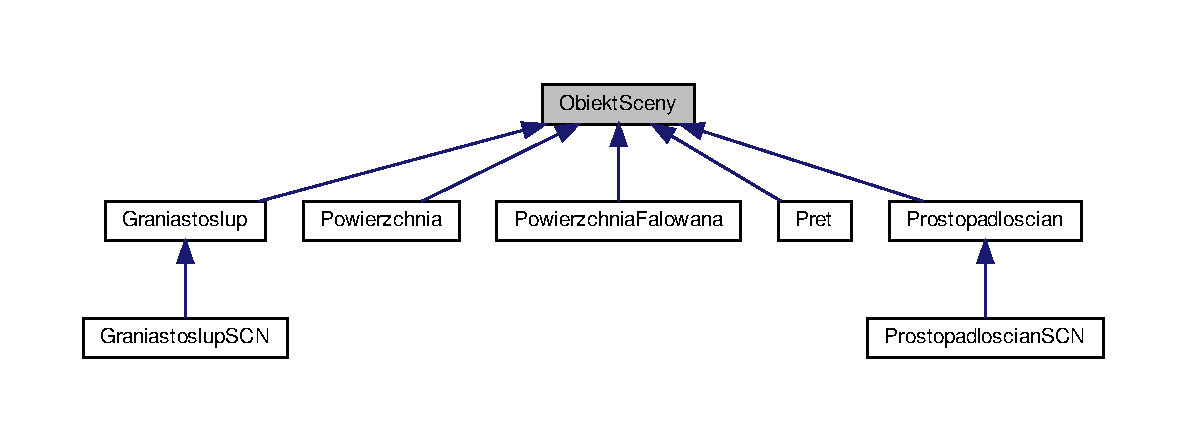
\includegraphics[width=350pt]{classObiektSceny__inherit__graph}
\end{center}
\end{figure}


Diagram współpracy dla Obiekt\+Sceny\+:\nopagebreak
\begin{figure}[H]
\begin{center}
\leavevmode
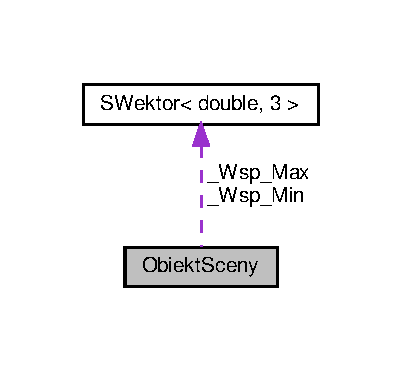
\includegraphics[width=193pt]{classObiektSceny__coll__graph}
\end{center}
\end{figure}
\subsection*{Metody publiczne}
\begin{DoxyCompactItemize}
\item 
\hyperlink{classObiektSceny_a3ac6cda78772edd23c39b3827c1695d8}{Obiekt\+Sceny} ()
\begin{DoxyCompactList}\small\item\em Konstruktor bezparametryczny. \end{DoxyCompactList}\item 
virtual \hyperlink{classObiektSceny_ab34aec7f37d73f5b1cc4d3268ac39af9}{$\sim$\+Obiekt\+Sceny} ()
\begin{DoxyCompactList}\small\item\em Destruktor. \end{DoxyCompactList}\item 
virtual bool \hyperlink{classObiektSceny_a24dd0332c0755d7155128639a9a3e2b4}{Wyznacz\+Wsp} ()=0
\begin{DoxyCompactList}\small\item\em Pierwotna wersja metodu umozliwiajacej wyznaczenie wspolrzednych skrajnych bryly. \end{DoxyCompactList}\item 
void \hyperlink{classObiektSceny_a84c19442a6a0757a1702e72effbb66d9}{Wybierz\+Plik\+Lok} (const char $\ast$Nazwa\+Pliku)
\begin{DoxyCompactList}\small\item\em Metoda umozliwia przypisanie obiektowi pliku. \end{DoxyCompactList}\item 
const std\+::string \hyperlink{classObiektSceny_abe634a96ea225f2e21b3dead5207d122}{Podaj\+Nazwe\+Pliku\+Lok} () const
\begin{DoxyCompactList}\small\item\em Metoda umozliwia pobranie nazwy przypisanego pliku. \end{DoxyCompactList}\item 
\hyperlink{classSWektor}{Wektor3D} const \hyperlink{classObiektSceny_ae6e0207ad7d44742b2973e92382619bb}{Podaj\+Wsp\+Max} () const
\begin{DoxyCompactList}\small\item\em Metoda umozliwia pobranie wartosci wspolrzednych maksymalnych. \end{DoxyCompactList}\item 
\hyperlink{classSWektor}{Wektor3D} \& \hyperlink{classObiektSceny_a5a66f5506b5e30e47040d31c8b751c7a}{Podaj\+Wsp\+Max} ()
\begin{DoxyCompactList}\small\item\em Metoda umozliwia pobranie i modyfikacje wartosci wspolrzednych maksymalnych. \end{DoxyCompactList}\item 
\hyperlink{classSWektor}{Wektor3D} const \hyperlink{classObiektSceny_a81f3173a7b40fdf30fd0488e470b86a6}{Podaj\+Wsp\+Min} () const
\begin{DoxyCompactList}\small\item\em Metoda umozliwia pobranie wartosci wspolrzednych minimalnych. \end{DoxyCompactList}\item 
\hyperlink{classSWektor}{Wektor3D} \& \hyperlink{classObiektSceny_a2f660e413ae6ed3eb0df7fac9881cf8a}{Podaj\+Wsp\+Min} ()
\begin{DoxyCompactList}\small\item\em Metoda umozliwia pobranie i modyfikacje wartosci wspolrzednych minimalnych. \end{DoxyCompactList}\end{DoxyCompactItemize}
\subsection*{Atrybuty prywatne}
\begin{DoxyCompactItemize}
\item 
std\+::string \hyperlink{classObiektSceny_abd56bb7b6b0db7ecef8055ce16131358}{\+\_\+\+Plik\+\_\+\+Wsp\+\_\+\+Lokalne}
\begin{DoxyCompactList}\small\item\em Pole przechowuje nazwe pliku z danymi lokalnymi. \end{DoxyCompactList}\item 
\hyperlink{classSWektor}{Wektor3D} \hyperlink{classObiektSceny_a09bfe62996fd73bbc7876524b211ce20}{\+\_\+\+Wsp\+\_\+\+Max}
\begin{DoxyCompactList}\small\item\em Pole przechowuje wspolrzedne maksymalne. \end{DoxyCompactList}\item 
\hyperlink{classSWektor}{Wektor3D} \hyperlink{classObiektSceny_a7395dc947479c40e29636cd8e8c5bfd3}{\+\_\+\+Wsp\+\_\+\+Min}
\begin{DoxyCompactList}\small\item\em Pole przechowuje wspolrzedne minimalne. \end{DoxyCompactList}\end{DoxyCompactItemize}


\subsection{Opis szczegółowy}
Definicja klasy \hyperlink{classObiektSceny}{Obiekt\+Sceny}. 

Definicję klasy \hyperlink{classObiektSceny}{Obiekt\+Sceny}, sluzacej do ogólnej interpretacji obiektów przestrzennych, mających okreslone wspolrzedne w ukladzie kartezjanskim. Ponadto obiekt zapamietuje wartosci swoich wspolrzednych skrajnych w celu umozliwienia bycia wykorzystanym do wykrycia kolizji. Klasa stanowi klase bazowa dla kazdej bryly reprezentowanej w pozostalej czesci programu. 

\subsection{Dokumentacja konstruktora i destruktora}
\mbox{\Hypertarget{classObiektSceny_a3ac6cda78772edd23c39b3827c1695d8}\label{classObiektSceny_a3ac6cda78772edd23c39b3827c1695d8}} 
\index{Obiekt\+Sceny@{Obiekt\+Sceny}!Obiekt\+Sceny@{Obiekt\+Sceny}}
\index{Obiekt\+Sceny@{Obiekt\+Sceny}!Obiekt\+Sceny@{Obiekt\+Sceny}}
\subsubsection{\texorpdfstring{Obiekt\+Sceny()}{ObiektSceny()}}
{\footnotesize\ttfamily Obiekt\+Sceny\+::\+Obiekt\+Sceny (\begin{DoxyParamCaption}{ }\end{DoxyParamCaption})\hspace{0.3cm}{\ttfamily [inline]}}



Konstruktor bezparametryczny. 

Konstruktor bezparametryczny wyswietlajacy komunikat o utworzeniu obiektu, w celu ulatwienia kontrolowania poprawnego wykorzystania pamieci \mbox{\Hypertarget{classObiektSceny_ab34aec7f37d73f5b1cc4d3268ac39af9}\label{classObiektSceny_ab34aec7f37d73f5b1cc4d3268ac39af9}} 
\index{Obiekt\+Sceny@{Obiekt\+Sceny}!````~Obiekt\+Sceny@{$\sim$\+Obiekt\+Sceny}}
\index{````~Obiekt\+Sceny@{$\sim$\+Obiekt\+Sceny}!Obiekt\+Sceny@{Obiekt\+Sceny}}
\subsubsection{\texorpdfstring{$\sim$\+Obiekt\+Sceny()}{~ObiektSceny()}}
{\footnotesize\ttfamily virtual Obiekt\+Sceny\+::$\sim$\+Obiekt\+Sceny (\begin{DoxyParamCaption}{ }\end{DoxyParamCaption})\hspace{0.3cm}{\ttfamily [inline]}, {\ttfamily [virtual]}}



Destruktor. 

Destruktor wyswietlajacy komunikat o usunieciu obiektu, w celu ulatwienia kontrolowania poprawnego wykorzystania pamieci 

\subsection{Dokumentacja funkcji składowych}
\mbox{\Hypertarget{classObiektSceny_abe634a96ea225f2e21b3dead5207d122}\label{classObiektSceny_abe634a96ea225f2e21b3dead5207d122}} 
\index{Obiekt\+Sceny@{Obiekt\+Sceny}!Podaj\+Nazwe\+Pliku\+Lok@{Podaj\+Nazwe\+Pliku\+Lok}}
\index{Podaj\+Nazwe\+Pliku\+Lok@{Podaj\+Nazwe\+Pliku\+Lok}!Obiekt\+Sceny@{Obiekt\+Sceny}}
\subsubsection{\texorpdfstring{Podaj\+Nazwe\+Pliku\+Lok()}{PodajNazwePlikuLok()}}
{\footnotesize\ttfamily const std\+::string Obiekt\+Sceny\+::\+Podaj\+Nazwe\+Pliku\+Lok (\begin{DoxyParamCaption}{ }\end{DoxyParamCaption}) const\hspace{0.3cm}{\ttfamily [inline]}}



Metoda umozliwia pobranie nazwy przypisanego pliku. 

Metoda umozliwia pobranie nazwy przypisanego pliku, w ktorym znajduja sie zadane wspolrzedne obiektu \begin{DoxyPrecond}{Warunek wstępny}
Nazwa pliku lokalnego musi byc wczesniej wybrana 
\end{DoxyPrecond}

\begin{DoxyRetVals}{Zwracane wartości}
{\em Parametr} & {\itshape \+\_\+\+Plik\+\_\+\+Wsp\+\_\+\+Lokalne} \\
\hline
\end{DoxyRetVals}
\mbox{\Hypertarget{classObiektSceny_ae6e0207ad7d44742b2973e92382619bb}\label{classObiektSceny_ae6e0207ad7d44742b2973e92382619bb}} 
\index{Obiekt\+Sceny@{Obiekt\+Sceny}!Podaj\+Wsp\+Max@{Podaj\+Wsp\+Max}}
\index{Podaj\+Wsp\+Max@{Podaj\+Wsp\+Max}!Obiekt\+Sceny@{Obiekt\+Sceny}}
\subsubsection{\texorpdfstring{Podaj\+Wsp\+Max()}{PodajWspMax()}\hspace{0.1cm}{\footnotesize\ttfamily [1/2]}}
{\footnotesize\ttfamily \hyperlink{classSWektor}{Wektor3D} const Obiekt\+Sceny\+::\+Podaj\+Wsp\+Max (\begin{DoxyParamCaption}{ }\end{DoxyParamCaption}) const\hspace{0.3cm}{\ttfamily [inline]}}



Metoda umozliwia pobranie wartosci wspolrzednych maksymalnych. 

Metoda umozliwia pobranie wartosci wspolrzednych maksymalnych \begin{DoxyPrecond}{Warunek wstępny}
Wartosc wspolrzednych musi byc wczesniej wyliczona 
\end{DoxyPrecond}

\begin{DoxyRetVals}{Zwracane wartości}
{\em Wektor3D} & {\itshape \+\_\+\+Wsp\+\_\+\+Max} \\
\hline
\end{DoxyRetVals}
\mbox{\Hypertarget{classObiektSceny_a5a66f5506b5e30e47040d31c8b751c7a}\label{classObiektSceny_a5a66f5506b5e30e47040d31c8b751c7a}} 
\index{Obiekt\+Sceny@{Obiekt\+Sceny}!Podaj\+Wsp\+Max@{Podaj\+Wsp\+Max}}
\index{Podaj\+Wsp\+Max@{Podaj\+Wsp\+Max}!Obiekt\+Sceny@{Obiekt\+Sceny}}
\subsubsection{\texorpdfstring{Podaj\+Wsp\+Max()}{PodajWspMax()}\hspace{0.1cm}{\footnotesize\ttfamily [2/2]}}
{\footnotesize\ttfamily \hyperlink{classSWektor}{Wektor3D}\& Obiekt\+Sceny\+::\+Podaj\+Wsp\+Max (\begin{DoxyParamCaption}{ }\end{DoxyParamCaption})\hspace{0.3cm}{\ttfamily [inline]}}



Metoda umozliwia pobranie i modyfikacje wartosci wspolrzednych maksymalnych. 

Metoda umozliwia pobranie i modyfikacje wartosci wspolrzednych maksymalnych \begin{DoxyPrecond}{Warunek wstępny}
Wartosc wspolrzednych musi byc wczesniej wyliczona 
\end{DoxyPrecond}

\begin{DoxyRetVals}{Zwracane wartości}
{\em Wektor3\+D\&} & {\itshape \+\_\+\+Wsp\+\_\+\+Max} \\
\hline
\end{DoxyRetVals}
\mbox{\Hypertarget{classObiektSceny_a81f3173a7b40fdf30fd0488e470b86a6}\label{classObiektSceny_a81f3173a7b40fdf30fd0488e470b86a6}} 
\index{Obiekt\+Sceny@{Obiekt\+Sceny}!Podaj\+Wsp\+Min@{Podaj\+Wsp\+Min}}
\index{Podaj\+Wsp\+Min@{Podaj\+Wsp\+Min}!Obiekt\+Sceny@{Obiekt\+Sceny}}
\subsubsection{\texorpdfstring{Podaj\+Wsp\+Min()}{PodajWspMin()}\hspace{0.1cm}{\footnotesize\ttfamily [1/2]}}
{\footnotesize\ttfamily \hyperlink{classSWektor}{Wektor3D} const Obiekt\+Sceny\+::\+Podaj\+Wsp\+Min (\begin{DoxyParamCaption}{ }\end{DoxyParamCaption}) const\hspace{0.3cm}{\ttfamily [inline]}}



Metoda umozliwia pobranie wartosci wspolrzednych minimalnych. 

Metoda umozliwia pobranie wartosci wspolrzednych minimalnych \begin{DoxyPrecond}{Warunek wstępny}
Wartosc wspolrzednych musi byc wczesniej wyliczona 
\end{DoxyPrecond}

\begin{DoxyRetVals}{Zwracane wartości}
{\em Wektor3D} & {\itshape \+\_\+\+Wsp\+\_\+\+Min} \\
\hline
\end{DoxyRetVals}
\mbox{\Hypertarget{classObiektSceny_a2f660e413ae6ed3eb0df7fac9881cf8a}\label{classObiektSceny_a2f660e413ae6ed3eb0df7fac9881cf8a}} 
\index{Obiekt\+Sceny@{Obiekt\+Sceny}!Podaj\+Wsp\+Min@{Podaj\+Wsp\+Min}}
\index{Podaj\+Wsp\+Min@{Podaj\+Wsp\+Min}!Obiekt\+Sceny@{Obiekt\+Sceny}}
\subsubsection{\texorpdfstring{Podaj\+Wsp\+Min()}{PodajWspMin()}\hspace{0.1cm}{\footnotesize\ttfamily [2/2]}}
{\footnotesize\ttfamily \hyperlink{classSWektor}{Wektor3D}\& Obiekt\+Sceny\+::\+Podaj\+Wsp\+Min (\begin{DoxyParamCaption}{ }\end{DoxyParamCaption})\hspace{0.3cm}{\ttfamily [inline]}}



Metoda umozliwia pobranie i modyfikacje wartosci wspolrzednych minimalnych. 

Metoda umozliwia pobranie i modyfikacje wartosci wspolrzednych minimalnych \begin{DoxyPrecond}{Warunek wstępny}
Wartosc wspolrzednych musi byc wczesniej wyliczona 
\end{DoxyPrecond}

\begin{DoxyRetVals}{Zwracane wartości}
{\em Wektor3\+D\&} & {\itshape \+\_\+\+Wsp\+\_\+\+Min} \\
\hline
\end{DoxyRetVals}
\mbox{\Hypertarget{classObiektSceny_a84c19442a6a0757a1702e72effbb66d9}\label{classObiektSceny_a84c19442a6a0757a1702e72effbb66d9}} 
\index{Obiekt\+Sceny@{Obiekt\+Sceny}!Wybierz\+Plik\+Lok@{Wybierz\+Plik\+Lok}}
\index{Wybierz\+Plik\+Lok@{Wybierz\+Plik\+Lok}!Obiekt\+Sceny@{Obiekt\+Sceny}}
\subsubsection{\texorpdfstring{Wybierz\+Plik\+Lok()}{WybierzPlikLok()}}
{\footnotesize\ttfamily void Obiekt\+Sceny\+::\+Wybierz\+Plik\+Lok (\begin{DoxyParamCaption}\item[{const char $\ast$}]{Nazwa\+Pliku }\end{DoxyParamCaption})\hspace{0.3cm}{\ttfamily [inline]}}



Metoda umozliwia przypisanie obiektowi pliku. 

Metoda umozliwia przypisanie obiektowi pliku ze wspolrzednymi lokalnymi


\begin{DoxyParams}[1]{Parametry}
\mbox{\tt in}  & {\em Nazwa\+Pliku} & -\/ Nazwa pliku ze wspolrzednymi lokalnymi \\
\hline
\end{DoxyParams}
\mbox{\Hypertarget{classObiektSceny_a24dd0332c0755d7155128639a9a3e2b4}\label{classObiektSceny_a24dd0332c0755d7155128639a9a3e2b4}} 
\index{Obiekt\+Sceny@{Obiekt\+Sceny}!Wyznacz\+Wsp@{Wyznacz\+Wsp}}
\index{Wyznacz\+Wsp@{Wyznacz\+Wsp}!Obiekt\+Sceny@{Obiekt\+Sceny}}
\subsubsection{\texorpdfstring{Wyznacz\+Wsp()}{WyznaczWsp()}}
{\footnotesize\ttfamily virtual bool Obiekt\+Sceny\+::\+Wyznacz\+Wsp (\begin{DoxyParamCaption}{ }\end{DoxyParamCaption})\hspace{0.3cm}{\ttfamily [pure virtual]}}



Pierwotna wersja metodu umozliwiajacej wyznaczenie wspolrzednych skrajnych bryly. 

Metoda umozliwia wyznaczenie wspolrzednych skrajnych bryly. W postaci zapisanej w tej klasie nie posiada ona kodu, gdyz nigdy nie bedzie ona wywolywana jako metoda samoistniejącej klasy bazowej -\/ w odpowiednich klasach pochodnych jest ona we wlasciwy sposob nadpisywana, aby poprawnie wyznaczac wspolrzedne skrajne dla roznych rodzajow bryl

\begin{DoxyPrecond}{Warunek wstępny}
Obiekt musi miec poprawnie zadane nazwy plikow ze wspolrzednymi 
\end{DoxyPrecond}

\begin{DoxyRetVals}{Zwracane wartości}
{\em true} & -\/ proces przebiegł pomyślnie \\
\hline
{\em false} & -\/ nie udało sie wyznaczyc wspolrzednych skrajnych \\
\hline
\end{DoxyRetVals}


Implementowany w \hyperlink{classGraniastoslupSCN_a096492db05264adae9306f5fb50cc3c9}{Graniastoslup\+S\+CN}, \hyperlink{classGraniastoslup_a786313962b174b9c25084e45e827f39b}{Graniastoslup}, \hyperlink{classProstopadloscian_a9d182fd3d875a1e3928c8972727be6fe}{Prostopadloscian}, \hyperlink{classProstopadloscianSCN_acdd4a5c10fb6347ad65b1a516ee83b01}{Prostopadloscian\+S\+CN}, \hyperlink{classPowierzchnia_a8e2453f9f7e8f92d77bd5608ef3de005}{Powierzchnia}, \hyperlink{classPowierzchniaFalowana_ae9f43f9acfb3db49fc9931ca4917e049}{Powierzchnia\+Falowana} i \hyperlink{classPret_affe3fdc72a84022eb5bbfddbf24cc2fc}{Pret}.



\subsection{Dokumentacja atrybutów składowych}
\mbox{\Hypertarget{classObiektSceny_abd56bb7b6b0db7ecef8055ce16131358}\label{classObiektSceny_abd56bb7b6b0db7ecef8055ce16131358}} 
\index{Obiekt\+Sceny@{Obiekt\+Sceny}!\+\_\+\+Plik\+\_\+\+Wsp\+\_\+\+Lokalne@{\+\_\+\+Plik\+\_\+\+Wsp\+\_\+\+Lokalne}}
\index{\+\_\+\+Plik\+\_\+\+Wsp\+\_\+\+Lokalne@{\+\_\+\+Plik\+\_\+\+Wsp\+\_\+\+Lokalne}!Obiekt\+Sceny@{Obiekt\+Sceny}}
\subsubsection{\texorpdfstring{\+\_\+\+Plik\+\_\+\+Wsp\+\_\+\+Lokalne}{\_Plik\_Wsp\_Lokalne}}
{\footnotesize\ttfamily std\+::string Obiekt\+Sceny\+::\+\_\+\+Plik\+\_\+\+Wsp\+\_\+\+Lokalne\hspace{0.3cm}{\ttfamily [private]}}



Pole przechowuje nazwe pliku z danymi lokalnymi. 

Pole przechowuje nazwe pliku z danymi lokalnymi \mbox{\Hypertarget{classObiektSceny_a09bfe62996fd73bbc7876524b211ce20}\label{classObiektSceny_a09bfe62996fd73bbc7876524b211ce20}} 
\index{Obiekt\+Sceny@{Obiekt\+Sceny}!\+\_\+\+Wsp\+\_\+\+Max@{\+\_\+\+Wsp\+\_\+\+Max}}
\index{\+\_\+\+Wsp\+\_\+\+Max@{\+\_\+\+Wsp\+\_\+\+Max}!Obiekt\+Sceny@{Obiekt\+Sceny}}
\subsubsection{\texorpdfstring{\+\_\+\+Wsp\+\_\+\+Max}{\_Wsp\_Max}}
{\footnotesize\ttfamily \hyperlink{classSWektor}{Wektor3D} Obiekt\+Sceny\+::\+\_\+\+Wsp\+\_\+\+Max\hspace{0.3cm}{\ttfamily [private]}}



Pole przechowuje wspolrzedne maksymalne. 

Pole przechowuje wspolrzedne maksymalne, tj. najbardziej wysuniete w strone dodatniej czesci kazdej osi ukladu \mbox{\Hypertarget{classObiektSceny_a7395dc947479c40e29636cd8e8c5bfd3}\label{classObiektSceny_a7395dc947479c40e29636cd8e8c5bfd3}} 
\index{Obiekt\+Sceny@{Obiekt\+Sceny}!\+\_\+\+Wsp\+\_\+\+Min@{\+\_\+\+Wsp\+\_\+\+Min}}
\index{\+\_\+\+Wsp\+\_\+\+Min@{\+\_\+\+Wsp\+\_\+\+Min}!Obiekt\+Sceny@{Obiekt\+Sceny}}
\subsubsection{\texorpdfstring{\+\_\+\+Wsp\+\_\+\+Min}{\_Wsp\_Min}}
{\footnotesize\ttfamily \hyperlink{classSWektor}{Wektor3D} Obiekt\+Sceny\+::\+\_\+\+Wsp\+\_\+\+Min\hspace{0.3cm}{\ttfamily [private]}}



Pole przechowuje wspolrzedne minimalne. 

Pole przechowuje wspolrzedne minimalne, tj. najbardziej wysuniete w strone ujemnej czesci kazdej osi ukladu 

Dokumentacja dla tej klasy została wygenerowana z pliku\+:\begin{DoxyCompactItemize}
\item 
inc/\hyperlink{ObiektSceny_8hh}{Obiekt\+Sceny.\+hh}\end{DoxyCompactItemize}

\hypertarget{classPowierzchnia}{}\section{Dokumentacja klasy Powierzchnia}
\label{classPowierzchnia}\index{Powierzchnia@{Powierzchnia}}


\hyperlink{classPowierzchnia}{Powierzchnia} jako obiekt graficzny.  




{\ttfamily \#include $<$Powierzchnia.\+hh$>$}



Diagram dziedziczenia dla Powierzchnia
\nopagebreak
\begin{figure}[H]
\begin{center}
\leavevmode
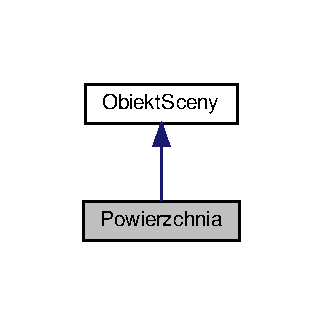
\includegraphics[width=155pt]{classPowierzchnia__inherit__graph}
\end{center}
\end{figure}


Diagram współpracy dla Powierzchnia\+:
\nopagebreak
\begin{figure}[H]
\begin{center}
\leavevmode
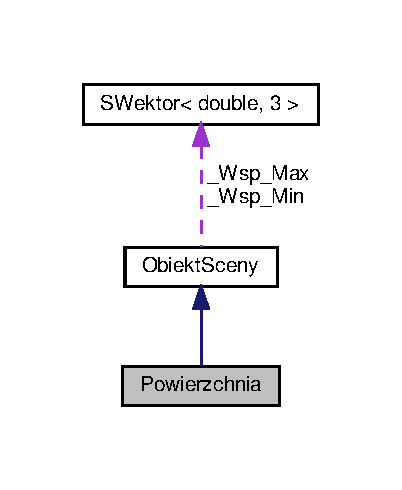
\includegraphics[width=193pt]{classPowierzchnia__coll__graph}
\end{center}
\end{figure}
\subsection*{Metody publiczne}
\begin{DoxyCompactItemize}
\item 
bool \hyperlink{classPowierzchnia_a8e2453f9f7e8f92d77bd5608ef3de005}{Wyznacz\+Wsp} () override
\begin{DoxyCompactList}\small\item\em Metoda umozliwia wyznaczenie wspolrzednych skrajnych bryly. \end{DoxyCompactList}\end{DoxyCompactItemize}


\subsection{Opis szczegółowy}
\hyperlink{classPowierzchnia}{Powierzchnia} jako obiekt graficzny. 

Klasa umożliwia interpretowanie obiektu jako powierzchni o okreslonych wspolrzednych w ukladzie kartezjanskim. 

\subsection{Dokumentacja funkcji składowych}
\mbox{\Hypertarget{classPowierzchnia_a8e2453f9f7e8f92d77bd5608ef3de005}\label{classPowierzchnia_a8e2453f9f7e8f92d77bd5608ef3de005}} 
\index{Powierzchnia@{Powierzchnia}!Wyznacz\+Wsp@{Wyznacz\+Wsp}}
\index{Wyznacz\+Wsp@{Wyznacz\+Wsp}!Powierzchnia@{Powierzchnia}}
\subsubsection{\texorpdfstring{Wyznacz\+Wsp()}{WyznaczWsp()}}
{\footnotesize\ttfamily bool Powierzchnia\+::\+Wyznacz\+Wsp (\begin{DoxyParamCaption}{ }\end{DoxyParamCaption})\hspace{0.3cm}{\ttfamily [override]}, {\ttfamily [virtual]}}



Metoda umozliwia wyznaczenie wspolrzednych skrajnych bryly. 

Metoda umozliwia wyznaczenie wspolrzednych skrajnych bryly, nadpisujac w odpowiedni sposob metode \hyperlink{classObiektSceny_a24dd0332c0755d7155128639a9a3e2b4}{Obiekt\+Sceny\+::\+Wyznacz\+Wsp()}

\begin{DoxyPrecond}{Warunek wstępny}
Obiekt musi miec poprawnie zadane nazwy plikow ze wspolrzednymi 
\end{DoxyPrecond}

\begin{DoxyRetVals}{Zwracane wartości}
{\em true} & -\/ proces przebiegł pomyślnie \\
\hline
{\em false} & -\/ nie udało sie wyznaczyc wspolrzednych skrajnych \\
\hline
\end{DoxyRetVals}


Implementuje \hyperlink{classObiektSceny_a24dd0332c0755d7155128639a9a3e2b4}{Obiekt\+Sceny}.



Dokumentacja dla tej klasy została wygenerowana z plików\+:\begin{DoxyCompactItemize}
\item 
inc/\hyperlink{Powierzchnia_8hh}{Powierzchnia.\+hh}\item 
src/\hyperlink{Powierzchnia_8cpp}{Powierzchnia.\+cpp}\end{DoxyCompactItemize}

\hypertarget{classPowierzchniaFalowana}{}\section{Dokumentacja klasy Powierzchnia\+Falowana}
\label{classPowierzchniaFalowana}\index{Powierzchnia\+Falowana@{Powierzchnia\+Falowana}}


\hyperlink{classPowierzchniaFalowana}{Powierzchnia\+Falowana} jako obiekt graficzny.  




{\ttfamily \#include $<$Powierzchnia\+Falowana.\+hh$>$}



Diagram dziedziczenia dla Powierzchnia\+Falowana
\nopagebreak
\begin{figure}[H]
\begin{center}
\leavevmode
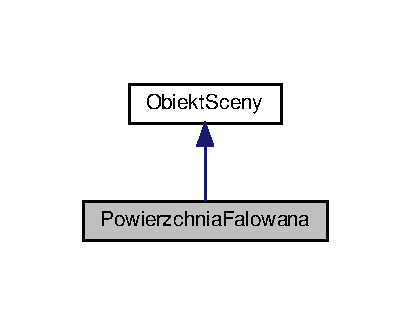
\includegraphics[width=197pt]{classPowierzchniaFalowana__inherit__graph}
\end{center}
\end{figure}


Diagram współpracy dla Powierzchnia\+Falowana\+:
\nopagebreak
\begin{figure}[H]
\begin{center}
\leavevmode
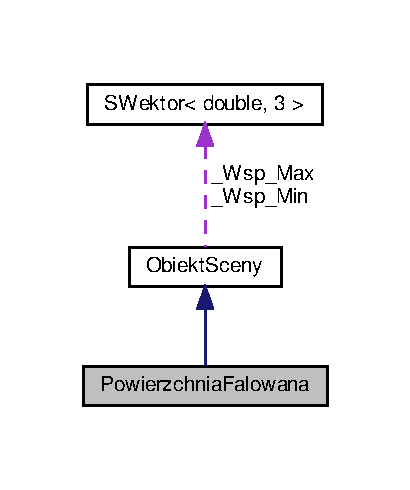
\includegraphics[width=197pt]{classPowierzchniaFalowana__coll__graph}
\end{center}
\end{figure}
\subsection*{Metody publiczne}
\begin{DoxyCompactItemize}
\item 
bool \hyperlink{classPowierzchniaFalowana_ae9f43f9acfb3db49fc9931ca4917e049}{Wyznacz\+Wsp} () override
\begin{DoxyCompactList}\small\item\em Metoda umozliwia wyznaczenie wspolrzednych skrajnych bryly. \end{DoxyCompactList}\end{DoxyCompactItemize}


\subsection{Opis szczegółowy}
\hyperlink{classPowierzchniaFalowana}{Powierzchnia\+Falowana} jako obiekt graficzny. 

Klasa umożliwia interpretowanie obiektu jako powierzchni falowanej o okreslonych wspolrzednych w ukladzie kartezjanskim. 

\subsection{Dokumentacja funkcji składowych}
\mbox{\Hypertarget{classPowierzchniaFalowana_ae9f43f9acfb3db49fc9931ca4917e049}\label{classPowierzchniaFalowana_ae9f43f9acfb3db49fc9931ca4917e049}} 
\index{Powierzchnia\+Falowana@{Powierzchnia\+Falowana}!Wyznacz\+Wsp@{Wyznacz\+Wsp}}
\index{Wyznacz\+Wsp@{Wyznacz\+Wsp}!Powierzchnia\+Falowana@{Powierzchnia\+Falowana}}
\subsubsection{\texorpdfstring{Wyznacz\+Wsp()}{WyznaczWsp()}}
{\footnotesize\ttfamily bool Powierzchnia\+Falowana\+::\+Wyznacz\+Wsp (\begin{DoxyParamCaption}{ }\end{DoxyParamCaption})\hspace{0.3cm}{\ttfamily [override]}, {\ttfamily [virtual]}}



Metoda umozliwia wyznaczenie wspolrzednych skrajnych bryly. 

Metoda umozliwia wyznaczenie wspolrzednych skrajnych bryly, nadpisujac w odpowiedni sposob metode \hyperlink{classObiektSceny_a24dd0332c0755d7155128639a9a3e2b4}{Obiekt\+Sceny\+::\+Wyznacz\+Wsp()}

\begin{DoxyPrecond}{Warunek wstępny}
Obiekt musi miec poprawnie zadane nazwy plikow ze wspolrzednymi 
\end{DoxyPrecond}

\begin{DoxyRetVals}{Zwracane wartości}
{\em true} & -\/ proces przebiegł pomyślnie \\
\hline
{\em false} & -\/ nie udało sie wyznaczyc wspolrzednych skrajnych \\
\hline
\end{DoxyRetVals}


Implementuje \hyperlink{classObiektSceny_a24dd0332c0755d7155128639a9a3e2b4}{Obiekt\+Sceny}.



Dokumentacja dla tej klasy została wygenerowana z plików\+:\begin{DoxyCompactItemize}
\item 
inc/\hyperlink{PowierzchniaFalowana_8hh}{Powierzchnia\+Falowana.\+hh}\item 
src/\hyperlink{PowierzchniaFalowana_8cpp}{Powierzchnia\+Falowana.\+cpp}\end{DoxyCompactItemize}

\hypertarget{classPret}{}\section{Dokumentacja klasy Pret}
\label{classPret}\index{Pret@{Pret}}


\hyperlink{classPret}{Pret} jako obiekt graficzny.  




{\ttfamily \#include $<$Pret.\+hh$>$}



Diagram dziedziczenia dla Pret
\nopagebreak
\begin{figure}[H]
\begin{center}
\leavevmode
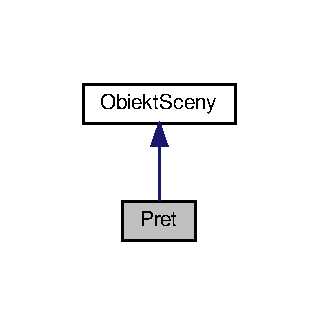
\includegraphics[width=153pt]{classPret__inherit__graph}
\end{center}
\end{figure}


Diagram współpracy dla Pret\+:
\nopagebreak
\begin{figure}[H]
\begin{center}
\leavevmode
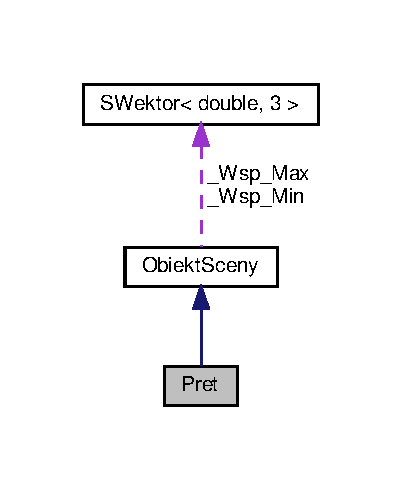
\includegraphics[width=193pt]{classPret__coll__graph}
\end{center}
\end{figure}
\subsection*{Metody publiczne}
\begin{DoxyCompactItemize}
\item 
bool \hyperlink{classPret_affe3fdc72a84022eb5bbfddbf24cc2fc}{Wyznacz\+Wsp} () override
\begin{DoxyCompactList}\small\item\em Metoda umozliwia wyznaczenie wspolrzednych skrajnych bryly. \end{DoxyCompactList}\end{DoxyCompactItemize}


\subsection{Opis szczegółowy}
\hyperlink{classPret}{Pret} jako obiekt graficzny. 

Klasa umożliwia interpretowanie obiektu jako preta o okreslonych wspolrzednych w ukladzie kartezjanskim. 

\subsection{Dokumentacja funkcji składowych}
\mbox{\Hypertarget{classPret_affe3fdc72a84022eb5bbfddbf24cc2fc}\label{classPret_affe3fdc72a84022eb5bbfddbf24cc2fc}} 
\index{Pret@{Pret}!Wyznacz\+Wsp@{Wyznacz\+Wsp}}
\index{Wyznacz\+Wsp@{Wyznacz\+Wsp}!Pret@{Pret}}
\subsubsection{\texorpdfstring{Wyznacz\+Wsp()}{WyznaczWsp()}}
{\footnotesize\ttfamily bool Pret\+::\+Wyznacz\+Wsp (\begin{DoxyParamCaption}{ }\end{DoxyParamCaption})\hspace{0.3cm}{\ttfamily [override]}, {\ttfamily [virtual]}}



Metoda umozliwia wyznaczenie wspolrzednych skrajnych bryly. 

Metoda umozliwia wyznaczenie wspolrzednych skrajnych bryly, nadpisujac w odpowiedni sposob metode \hyperlink{classObiektSceny_a24dd0332c0755d7155128639a9a3e2b4}{Obiekt\+Sceny\+::\+Wyznacz\+Wsp()}

\begin{DoxyPrecond}{Warunek wstępny}
Obiekt musi miec poprawnie zadane nazwy plikow ze wspolrzednymi 
\end{DoxyPrecond}

\begin{DoxyRetVals}{Zwracane wartości}
{\em true} & -\/ proces przebiegł pomyślnie \\
\hline
{\em false} & -\/ nie udało sie wyznaczyc wspolrzednych skrajnych \\
\hline
\end{DoxyRetVals}


Implementuje \hyperlink{classObiektSceny_a24dd0332c0755d7155128639a9a3e2b4}{Obiekt\+Sceny}.



Dokumentacja dla tej klasy została wygenerowana z plików\+:\begin{DoxyCompactItemize}
\item 
inc/\hyperlink{Pret_8hh}{Pret.\+hh}\item 
src/\hyperlink{Pret_8cpp}{Pret.\+cpp}\end{DoxyCompactItemize}

\hypertarget{classProstopadloscian}{}\section{Dokumentacja klasy Prostopadloscian}
\label{classProstopadloscian}\index{Prostopadloscian@{Prostopadloscian}}


\hyperlink{classProstopadloscian}{Prostopadloscian} jako bryla przestrzenna o promieniu i srodku lokalnym.  




{\ttfamily \#include $<$Prostopadloscian.\+hh$>$}



Diagram dziedziczenia dla Prostopadloscian
\nopagebreak
\begin{figure}[H]
\begin{center}
\leavevmode
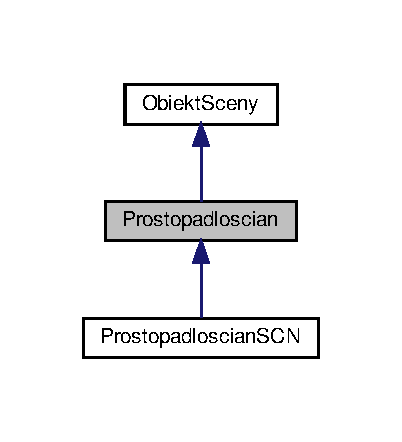
\includegraphics[width=193pt]{classProstopadloscian__inherit__graph}
\end{center}
\end{figure}


Diagram współpracy dla Prostopadloscian\+:
\nopagebreak
\begin{figure}[H]
\begin{center}
\leavevmode
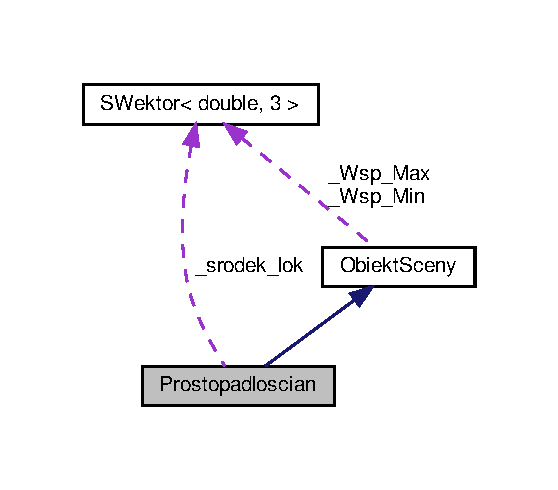
\includegraphics[width=268pt]{classProstopadloscian__coll__graph}
\end{center}
\end{figure}
\subsection*{Metody publiczne}
\begin{DoxyCompactItemize}
\item 
\hyperlink{classProstopadloscian_a432b8df2af37ba1a3596f500824eaffe}{Prostopadloscian} ()
\begin{DoxyCompactList}\small\item\em Konstruktor bezparametryczny. \end{DoxyCompactList}\item 
void \hyperlink{classProstopadloscian_a148c8e01a4610bd61081b49789d3bc71}{Wyznacz\+\_\+\+Promien\+\_\+i\+\_\+\+Srodek} ()
\begin{DoxyCompactList}\small\item\em Metoda umozliwia okreslenie promienia i srodka. \end{DoxyCompactList}\item 
unsigned int const \hyperlink{classProstopadloscian_ae6b1528649b6034209ac763cc5881527}{Podaj\+Promien} () const
\begin{DoxyCompactList}\small\item\em Metoda umozliwia pobranie dlugosci promienia. \end{DoxyCompactList}\item 
\hyperlink{classSWektor}{Wektor3D} const \hyperlink{classProstopadloscian_ab9c86b023b990acffe00891c17ee596c}{Podaj\+Srodek\+Lok} () const
\begin{DoxyCompactList}\small\item\em Metoda umozliwia pobranie wspolrzednych srodka. \end{DoxyCompactList}\item 
virtual bool \hyperlink{classProstopadloscian_a9d182fd3d875a1e3928c8972727be6fe}{Wyznacz\+Wsp} () override
\begin{DoxyCompactList}\small\item\em Metoda umozliwia wyznaczenie wspolrzednych skrajnych bryly. \end{DoxyCompactList}\end{DoxyCompactItemize}
\subsection*{Atrybuty prywatne}
\begin{DoxyCompactItemize}
\item 
unsigned int \hyperlink{classProstopadloscian_a06187a64d02fff11fc99e749abcef125}{\+\_\+promien}
\begin{DoxyCompactList}\small\item\em Pole przechowuje dlugosc promienia. \end{DoxyCompactList}\item 
\hyperlink{classSWektor}{Wektor3D} \hyperlink{classProstopadloscian_a3aac0fbd53f5add1fe4e802204e7f609}{\+\_\+srodek\+\_\+lok}
\begin{DoxyCompactList}\small\item\em Pole przechowuje wspolrzedne srodka. \end{DoxyCompactList}\end{DoxyCompactItemize}


\subsection{Opis szczegółowy}
\hyperlink{classProstopadloscian}{Prostopadloscian} jako bryla przestrzenna o promieniu i srodku lokalnym. 

Definicja klasy \hyperlink{classProstopadloscian}{Prostopadloscian}, sluzacej do interpretacji zadanego obiektu jako prostopadloscianu majacego okreslone wspolrzedne w ukladzie kartezjanskim. Ponadto obiekt zapamietuje wartosc swojego promienia oraz lokalne polozenie swojego srodka. 

\subsection{Dokumentacja konstruktora i destruktora}
\mbox{\Hypertarget{classProstopadloscian_a432b8df2af37ba1a3596f500824eaffe}\label{classProstopadloscian_a432b8df2af37ba1a3596f500824eaffe}} 
\index{Prostopadloscian@{Prostopadloscian}!Prostopadloscian@{Prostopadloscian}}
\index{Prostopadloscian@{Prostopadloscian}!Prostopadloscian@{Prostopadloscian}}
\subsubsection{\texorpdfstring{Prostopadloscian()}{Prostopadloscian()}}
{\footnotesize\ttfamily Prostopadloscian\+::\+Prostopadloscian (\begin{DoxyParamCaption}{ }\end{DoxyParamCaption})\hspace{0.3cm}{\ttfamily [inline]}}



Konstruktor bezparametryczny. 

Konstruktor bezparametryczny inicjalizujacy poczatkowa dlugosc promienia 

\subsection{Dokumentacja funkcji składowych}
\mbox{\Hypertarget{classProstopadloscian_ae6b1528649b6034209ac763cc5881527}\label{classProstopadloscian_ae6b1528649b6034209ac763cc5881527}} 
\index{Prostopadloscian@{Prostopadloscian}!Podaj\+Promien@{Podaj\+Promien}}
\index{Podaj\+Promien@{Podaj\+Promien}!Prostopadloscian@{Prostopadloscian}}
\subsubsection{\texorpdfstring{Podaj\+Promien()}{PodajPromien()}}
{\footnotesize\ttfamily unsigned int const Prostopadloscian\+::\+Podaj\+Promien (\begin{DoxyParamCaption}{ }\end{DoxyParamCaption}) const\hspace{0.3cm}{\ttfamily [inline]}}



Metoda umozliwia pobranie dlugosci promienia. 

Metoda umozliwia pobranie wartosci promienia \begin{DoxyPrecond}{Warunek wstępny}
Wartosc promienia musi byc wczesniej wyliczona 
\end{DoxyPrecond}

\begin{DoxyRetVals}{Zwracane wartości}
{\em Wartosc} & {\itshape \+\_\+promien} \\
\hline
\end{DoxyRetVals}
\mbox{\Hypertarget{classProstopadloscian_ab9c86b023b990acffe00891c17ee596c}\label{classProstopadloscian_ab9c86b023b990acffe00891c17ee596c}} 
\index{Prostopadloscian@{Prostopadloscian}!Podaj\+Srodek\+Lok@{Podaj\+Srodek\+Lok}}
\index{Podaj\+Srodek\+Lok@{Podaj\+Srodek\+Lok}!Prostopadloscian@{Prostopadloscian}}
\subsubsection{\texorpdfstring{Podaj\+Srodek\+Lok()}{PodajSrodekLok()}}
{\footnotesize\ttfamily \hyperlink{classSWektor}{Wektor3D} const Prostopadloscian\+::\+Podaj\+Srodek\+Lok (\begin{DoxyParamCaption}{ }\end{DoxyParamCaption}) const\hspace{0.3cm}{\ttfamily [inline]}}



Metoda umozliwia pobranie wspolrzednych srodka. 

Metoda umozliwia pobranie wartosci wspolrzednych srodka lokalnego bryly 
\begin{DoxyRetVals}{Zwracane wartości}
{\em Wektor3D} & {\itshape \+\_\+srodek\+\_\+lok} \\
\hline
\end{DoxyRetVals}
\mbox{\Hypertarget{classProstopadloscian_a148c8e01a4610bd61081b49789d3bc71}\label{classProstopadloscian_a148c8e01a4610bd61081b49789d3bc71}} 
\index{Prostopadloscian@{Prostopadloscian}!Wyznacz\+\_\+\+Promien\+\_\+i\+\_\+\+Srodek@{Wyznacz\+\_\+\+Promien\+\_\+i\+\_\+\+Srodek}}
\index{Wyznacz\+\_\+\+Promien\+\_\+i\+\_\+\+Srodek@{Wyznacz\+\_\+\+Promien\+\_\+i\+\_\+\+Srodek}!Prostopadloscian@{Prostopadloscian}}
\subsubsection{\texorpdfstring{Wyznacz\+\_\+\+Promien\+\_\+i\+\_\+\+Srodek()}{Wyznacz\_Promien\_i\_Srodek()}}
{\footnotesize\ttfamily void Prostopadloscian\+::\+Wyznacz\+\_\+\+Promien\+\_\+i\+\_\+\+Srodek (\begin{DoxyParamCaption}{ }\end{DoxyParamCaption})}



Metoda umozliwia okreslenie promienia i srodka. 

Metoda umozliwia wyznaczenie wspolrzednych srodka lokalnego oraz dlugosci promienia bryly, a nastepnie zapamietanie ich wartosci w polach obiektu \begin{DoxyPrecond}{Warunek wstępny}
Wspolrzedne obiektu musza byc wczesniej poprawnie zapisane w pliku, ktorego nazwa zapisana jest przez pole {\itshape \+\_\+\+Plik\+\_\+\+Wsp\+\_\+\+Lokalne} 
\end{DoxyPrecond}
\mbox{\Hypertarget{classProstopadloscian_a9d182fd3d875a1e3928c8972727be6fe}\label{classProstopadloscian_a9d182fd3d875a1e3928c8972727be6fe}} 
\index{Prostopadloscian@{Prostopadloscian}!Wyznacz\+Wsp@{Wyznacz\+Wsp}}
\index{Wyznacz\+Wsp@{Wyznacz\+Wsp}!Prostopadloscian@{Prostopadloscian}}
\subsubsection{\texorpdfstring{Wyznacz\+Wsp()}{WyznaczWsp()}}
{\footnotesize\ttfamily bool Prostopadloscian\+::\+Wyznacz\+Wsp (\begin{DoxyParamCaption}{ }\end{DoxyParamCaption})\hspace{0.3cm}{\ttfamily [override]}, {\ttfamily [virtual]}}



Metoda umozliwia wyznaczenie wspolrzednych skrajnych bryly. 

Metoda umozliwia wyznaczenie wspolrzednych skrajnych bryly, nadpisujac w odpowiedni sposob metode \hyperlink{classObiektSceny_a24dd0332c0755d7155128639a9a3e2b4}{Obiekt\+Sceny\+::\+Wyznacz\+Wsp()}

\begin{DoxyPrecond}{Warunek wstępny}
Obiekt musi miec poprawnie zadane nazwy plikow ze wspolrzednymi 
\end{DoxyPrecond}

\begin{DoxyRetVals}{Zwracane wartości}
{\em true} & -\/ proces przebiegł pomyślnie \\
\hline
{\em false} & -\/ nie udało sie wyznaczyc wspolrzednych skrajnych \\
\hline
\end{DoxyRetVals}


Implementuje \hyperlink{classObiektSceny_a24dd0332c0755d7155128639a9a3e2b4}{Obiekt\+Sceny}.



Reimplementowana w \hyperlink{classProstopadloscianSCN_acdd4a5c10fb6347ad65b1a516ee83b01}{Prostopadloscian\+S\+CN}.



\subsection{Dokumentacja atrybutów składowych}
\mbox{\Hypertarget{classProstopadloscian_a06187a64d02fff11fc99e749abcef125}\label{classProstopadloscian_a06187a64d02fff11fc99e749abcef125}} 
\index{Prostopadloscian@{Prostopadloscian}!\+\_\+promien@{\+\_\+promien}}
\index{\+\_\+promien@{\+\_\+promien}!Prostopadloscian@{Prostopadloscian}}
\subsubsection{\texorpdfstring{\+\_\+promien}{\_promien}}
{\footnotesize\ttfamily unsigned int Prostopadloscian\+::\+\_\+promien\hspace{0.3cm}{\ttfamily [private]}}



Pole przechowuje dlugosc promienia. 

Pole przechowuje dlugosc promienia bryly \mbox{\Hypertarget{classProstopadloscian_a3aac0fbd53f5add1fe4e802204e7f609}\label{classProstopadloscian_a3aac0fbd53f5add1fe4e802204e7f609}} 
\index{Prostopadloscian@{Prostopadloscian}!\+\_\+srodek\+\_\+lok@{\+\_\+srodek\+\_\+lok}}
\index{\+\_\+srodek\+\_\+lok@{\+\_\+srodek\+\_\+lok}!Prostopadloscian@{Prostopadloscian}}
\subsubsection{\texorpdfstring{\+\_\+srodek\+\_\+lok}{\_srodek\_lok}}
{\footnotesize\ttfamily \hyperlink{classSWektor}{Wektor3D} Prostopadloscian\+::\+\_\+srodek\+\_\+lok\hspace{0.3cm}{\ttfamily [private]}}



Pole przechowuje wspolrzedne srodka. 

Pole przechowuje pierwotne wspolrzedne srodka bryly 

Dokumentacja dla tej klasy została wygenerowana z plików\+:\begin{DoxyCompactItemize}
\item 
inc/\hyperlink{Prostopadloscian_8hh}{Prostopadloscian.\+hh}\item 
src/\hyperlink{Prostopadloscian_8cpp}{Prostopadloscian.\+cpp}\end{DoxyCompactItemize}

\hypertarget{classProstopadloscianSCN}{}\section{Dokumentacja klasy Prostopadloscian\+S\+CN}
\label{classProstopadloscianSCN}\index{Prostopadloscian\+S\+CN@{Prostopadloscian\+S\+CN}}


\hyperlink{classProstopadloscianSCN}{Prostopadloscian\+S\+CN} jako \hyperlink{classProstopadloscian}{Prostopadloscian} w ukladzie globalnym.  




{\ttfamily \#include $<$Prostopadloscian\+S\+C\+N.\+hh$>$}



Diagram dziedziczenia dla Prostopadloscian\+S\+CN
\nopagebreak
\begin{figure}[H]
\begin{center}
\leavevmode
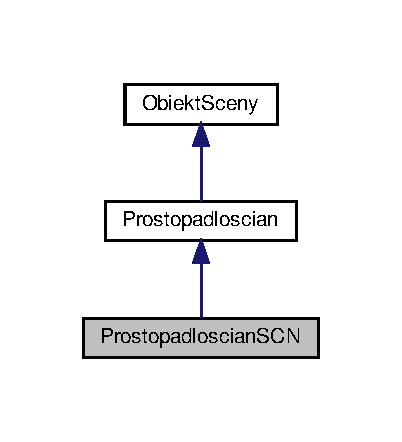
\includegraphics[width=193pt]{classProstopadloscianSCN__inherit__graph}
\end{center}
\end{figure}


Diagram współpracy dla Prostopadloscian\+S\+CN\+:
\nopagebreak
\begin{figure}[H]
\begin{center}
\leavevmode
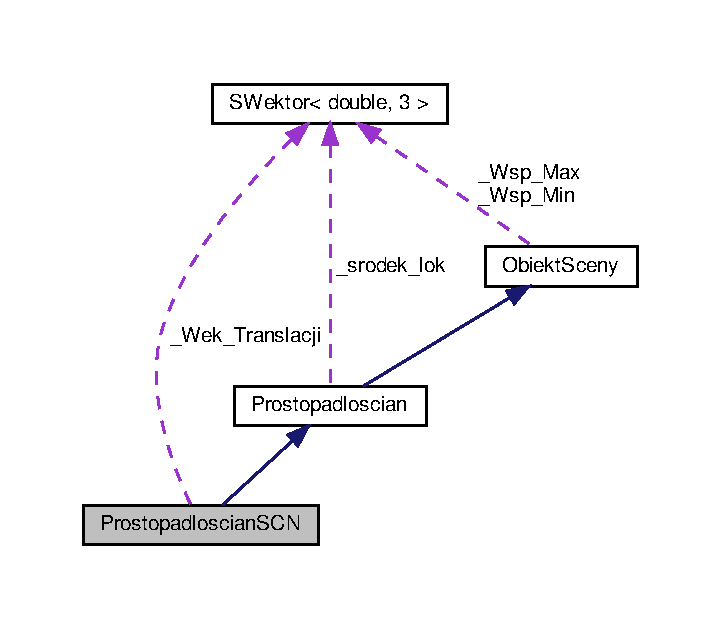
\includegraphics[width=346pt]{classProstopadloscianSCN__coll__graph}
\end{center}
\end{figure}
\subsection*{Metody publiczne}
\begin{DoxyCompactItemize}
\item 
\hyperlink{classProstopadloscianSCN_a8288627cc69c54812c06be68950615f5}{Prostopadloscian\+S\+CN} ()
\begin{DoxyCompactList}\small\item\em Konstruktor obiektu \hyperlink{classProstopadloscianSCN}{Prostopadloscian\+S\+CN}. \end{DoxyCompactList}\item 
void \hyperlink{classProstopadloscianSCN_aedacd1e8362390241287296f5107d493}{Wybierz\+Plik\+Glob} (const char $\ast$Nazwa\+Pliku)
\begin{DoxyCompactList}\small\item\em Metoda umozliwia przypisanie obiektowi pliku ze wspolrzednymi globalnymi. \end{DoxyCompactList}\item 
const std\+::string \hyperlink{classProstopadloscianSCN_a203c4bf0a0e65ed9896199e7a6dc498b}{Podaj\+Nazwe\+Pliku\+Glob} () const
\begin{DoxyCompactList}\small\item\em Metoda umozliwia pobranie nazwy przypisanego pliku ze wspolrzednymi globalnymi. \end{DoxyCompactList}\item 
virtual bool \hyperlink{classProstopadloscianSCN_acdd4a5c10fb6347ad65b1a516ee83b01}{Wyznacz\+Wsp} () override
\begin{DoxyCompactList}\small\item\em Metoda umozliwia wyznaczenie obecnych wspolrzednych skrajnych bryly. \end{DoxyCompactList}\item 
bool \hyperlink{classProstopadloscianSCN_ada3c51233b828c9ee8466a1c4270906b}{Oblicz\+Globalne} () const
\begin{DoxyCompactList}\small\item\em Realizuje przeksztalcenie wspolrzednych lokalnych do ukladu globalnego. \end{DoxyCompactList}\item 
bool \hyperlink{classProstopadloscianSCN_a397c310956e20068dc3588ee4d4a9c87}{Wybierz\+Pliki} (const char $\ast$Nazwa\+Pliku\+We, const char $\ast$Nazwa\+Pliku\+Wy)
\begin{DoxyCompactList}\small\item\em Metoda umozliwia przypisanie obiektowi dwoch plikow. \end{DoxyCompactList}\item 
void \hyperlink{classProstopadloscianSCN_a1f9b715a50dd0e84fb6391dcccc962e8}{Zmien\+\_\+o\+\_\+kat} (int kat)
\begin{DoxyCompactList}\small\item\em Metoda umozliwia zmiane orientacji bryly wokol osi OZ. \end{DoxyCompactList}\item 
void \hyperlink{classProstopadloscianSCN_afa54ddf8455489f51aa945afcafee27f}{Zmien\+\_\+o\+\_\+translacje} (\hyperlink{classSWektor}{Wektor3D} Translacja)
\begin{DoxyCompactList}\small\item\em Metoda umozliwia zmiane polozenia bryly. \end{DoxyCompactList}\item 
int const \hyperlink{classProstopadloscianSCN_a4d1aaf928130a4d48a0cdc9ab79917be}{Podaj\+Kat\+Orientacji} () const
\begin{DoxyCompactList}\small\item\em Metoda umozliwia pobranie wartosci kata orientacji bryly. \end{DoxyCompactList}\item 
\hyperlink{classSWektor}{Wektor3D} const \hyperlink{classProstopadloscianSCN_ae0157d734326422f325c9af1894292ed}{Podaj\+Polozenie} () const
\begin{DoxyCompactList}\small\item\em Metoda umozliwia pobranie wartosci wektora polozenia bryly. \end{DoxyCompactList}\end{DoxyCompactItemize}
\subsection*{Atrybuty prywatne}
\begin{DoxyCompactItemize}
\item 
std\+::string \hyperlink{classProstopadloscianSCN_ab6ed51a7c62d80bca489497ad60a861c}{\+\_\+\+Plik\+\_\+\+Wsp\+\_\+\+Globalne}
\begin{DoxyCompactList}\small\item\em Pole przechowuje nazwe pliku z danymi globalnymi. \end{DoxyCompactList}\item 
int \hyperlink{classProstopadloscianSCN_ab47d8efc8b2817cabf5ea70915a8f5dc}{\+\_\+\+Kat\+\_\+\+Orientacji}
\begin{DoxyCompactList}\small\item\em Pole przechowuje miare kata orientacji. \end{DoxyCompactList}\item 
\hyperlink{classSWektor}{Wektor3D} \hyperlink{classProstopadloscianSCN_a4ca4e6e7fe68e627d4a3f6373f1482ad}{\+\_\+\+Wek\+\_\+\+Translacji}
\begin{DoxyCompactList}\small\item\em Pole przechowuje wektor translacji bryly. \end{DoxyCompactList}\end{DoxyCompactItemize}


\subsection{Opis szczegółowy}
\hyperlink{classProstopadloscianSCN}{Prostopadloscian\+S\+CN} jako \hyperlink{classProstopadloscian}{Prostopadloscian} w ukladzie globalnym. 

Definicja klasy \hyperlink{classProstopadloscianSCN}{Prostopadloscian\+S\+CN}, sluzacej do interpretacji zadanego prostopadloscianu jako obiektu rozbudowanego o mozliwosc okreslenia orientacji i przesuniecia w ukladzie globalnym 

\subsection{Dokumentacja konstruktora i destruktora}
\mbox{\Hypertarget{classProstopadloscianSCN_a8288627cc69c54812c06be68950615f5}\label{classProstopadloscianSCN_a8288627cc69c54812c06be68950615f5}} 
\index{Prostopadloscian\+S\+CN@{Prostopadloscian\+S\+CN}!Prostopadloscian\+S\+CN@{Prostopadloscian\+S\+CN}}
\index{Prostopadloscian\+S\+CN@{Prostopadloscian\+S\+CN}!Prostopadloscian\+S\+CN@{Prostopadloscian\+S\+CN}}
\subsubsection{\texorpdfstring{Prostopadloscian\+S\+C\+N()}{ProstopadloscianSCN()}}
{\footnotesize\ttfamily Prostopadloscian\+S\+C\+N\+::\+Prostopadloscian\+S\+CN (\begin{DoxyParamCaption}{ }\end{DoxyParamCaption})\hspace{0.3cm}{\ttfamily [inline]}}



Konstruktor obiektu \hyperlink{classProstopadloscianSCN}{Prostopadloscian\+S\+CN}. 

Konstruktor bezparametryczny obiektu \hyperlink{classProstopadloscianSCN}{Prostopadloscian\+S\+CN}, ustawiajacy domyslna wartosc kata orientacji bryly na 0 

\subsection{Dokumentacja funkcji składowych}
\mbox{\Hypertarget{classProstopadloscianSCN_ada3c51233b828c9ee8466a1c4270906b}\label{classProstopadloscianSCN_ada3c51233b828c9ee8466a1c4270906b}} 
\index{Prostopadloscian\+S\+CN@{Prostopadloscian\+S\+CN}!Oblicz\+Globalne@{Oblicz\+Globalne}}
\index{Oblicz\+Globalne@{Oblicz\+Globalne}!Prostopadloscian\+S\+CN@{Prostopadloscian\+S\+CN}}
\subsubsection{\texorpdfstring{Oblicz\+Globalne()}{ObliczGlobalne()}}
{\footnotesize\ttfamily bool Prostopadloscian\+S\+C\+N\+::\+Oblicz\+Globalne (\begin{DoxyParamCaption}{ }\end{DoxyParamCaption}) const}



Realizuje przeksztalcenie wspolrzednych lokalnych do ukladu globalnego. 

Realizuje przeksztalcenie wspolrzednych lokalnych do ukladu globalnego biorac pod uwage kat orientacji oraz wektor translacji bryly

\begin{DoxyPrecond}{Warunek wstępny}
Obiekt musi miec poprawnie zadane nazwy plikow ze wspolrzednymi 
\end{DoxyPrecond}

\begin{DoxyRetVals}{Zwracane wartości}
{\em true} & -\/ operacja przebiegla pomyslnie \\
\hline
{\em false} & -\/ nie udalo sie okreslic wspolrzednych globalnych -\/ blad prawidlowego odczytania wspolrzednych z pliku {\itshape \+\_\+\+Plik\+\_\+\+Wsp\+\_\+\+Lokalne} lub blad zapisu do pliku {\itshape \+\_\+\+Plik\+\_\+\+Wsp\+\_\+\+Globalne} \\
\hline
\end{DoxyRetVals}
\mbox{\Hypertarget{classProstopadloscianSCN_a4d1aaf928130a4d48a0cdc9ab79917be}\label{classProstopadloscianSCN_a4d1aaf928130a4d48a0cdc9ab79917be}} 
\index{Prostopadloscian\+S\+CN@{Prostopadloscian\+S\+CN}!Podaj\+Kat\+Orientacji@{Podaj\+Kat\+Orientacji}}
\index{Podaj\+Kat\+Orientacji@{Podaj\+Kat\+Orientacji}!Prostopadloscian\+S\+CN@{Prostopadloscian\+S\+CN}}
\subsubsection{\texorpdfstring{Podaj\+Kat\+Orientacji()}{PodajKatOrientacji()}}
{\footnotesize\ttfamily int const Prostopadloscian\+S\+C\+N\+::\+Podaj\+Kat\+Orientacji (\begin{DoxyParamCaption}{ }\end{DoxyParamCaption}) const\hspace{0.3cm}{\ttfamily [inline]}}



Metoda umozliwia pobranie wartosci kata orientacji bryly. 

Metoda umozliwia pobranie wartosci okreslonego kata orientacji bryly 
\begin{DoxyRetVals}{Zwracane wartości}
{\em Wartosc} & {\itshape \+\_\+\+Kat\+\_\+\+Orientacji} \\
\hline
\end{DoxyRetVals}
\mbox{\Hypertarget{classProstopadloscianSCN_a203c4bf0a0e65ed9896199e7a6dc498b}\label{classProstopadloscianSCN_a203c4bf0a0e65ed9896199e7a6dc498b}} 
\index{Prostopadloscian\+S\+CN@{Prostopadloscian\+S\+CN}!Podaj\+Nazwe\+Pliku\+Glob@{Podaj\+Nazwe\+Pliku\+Glob}}
\index{Podaj\+Nazwe\+Pliku\+Glob@{Podaj\+Nazwe\+Pliku\+Glob}!Prostopadloscian\+S\+CN@{Prostopadloscian\+S\+CN}}
\subsubsection{\texorpdfstring{Podaj\+Nazwe\+Pliku\+Glob()}{PodajNazwePlikuGlob()}}
{\footnotesize\ttfamily const std\+::string Prostopadloscian\+S\+C\+N\+::\+Podaj\+Nazwe\+Pliku\+Glob (\begin{DoxyParamCaption}{ }\end{DoxyParamCaption}) const\hspace{0.3cm}{\ttfamily [inline]}}



Metoda umozliwia pobranie nazwy przypisanego pliku ze wspolrzednymi globalnymi. 

Metoda umozliwia pobranie nazwy przypisanego pliku, w ktorym beda znajdowac sie wyliczone wspolrzedne globalne obiektu \begin{DoxyPrecond}{Warunek wstępny}
Nazwa pliku ze wspolrzednymi globalnymi musi byc wczesniej okreslona 
\end{DoxyPrecond}

\begin{DoxyRetVals}{Zwracane wartości}
{\em Parametr} & {\itshape \+\_\+\+Plik\+\_\+\+Wsp\+\_\+\+Globalne} \\
\hline
\end{DoxyRetVals}
\mbox{\Hypertarget{classProstopadloscianSCN_ae0157d734326422f325c9af1894292ed}\label{classProstopadloscianSCN_ae0157d734326422f325c9af1894292ed}} 
\index{Prostopadloscian\+S\+CN@{Prostopadloscian\+S\+CN}!Podaj\+Polozenie@{Podaj\+Polozenie}}
\index{Podaj\+Polozenie@{Podaj\+Polozenie}!Prostopadloscian\+S\+CN@{Prostopadloscian\+S\+CN}}
\subsubsection{\texorpdfstring{Podaj\+Polozenie()}{PodajPolozenie()}}
{\footnotesize\ttfamily \hyperlink{classSWektor}{Wektor3D} const Prostopadloscian\+S\+C\+N\+::\+Podaj\+Polozenie (\begin{DoxyParamCaption}{ }\end{DoxyParamCaption}) const\hspace{0.3cm}{\ttfamily [inline]}}



Metoda umozliwia pobranie wartosci wektora polozenia bryly. 

Metoda umozliwia pobranie wartosci okreslonego wektora polozenia bryly 
\begin{DoxyRetVals}{Zwracane wartości}
{\em Wektor3D} & {\itshape \+\_\+\+Wek\+\_\+\+Translacji} \\
\hline
\end{DoxyRetVals}
\mbox{\Hypertarget{classProstopadloscianSCN_aedacd1e8362390241287296f5107d493}\label{classProstopadloscianSCN_aedacd1e8362390241287296f5107d493}} 
\index{Prostopadloscian\+S\+CN@{Prostopadloscian\+S\+CN}!Wybierz\+Plik\+Glob@{Wybierz\+Plik\+Glob}}
\index{Wybierz\+Plik\+Glob@{Wybierz\+Plik\+Glob}!Prostopadloscian\+S\+CN@{Prostopadloscian\+S\+CN}}
\subsubsection{\texorpdfstring{Wybierz\+Plik\+Glob()}{WybierzPlikGlob()}}
{\footnotesize\ttfamily void Prostopadloscian\+S\+C\+N\+::\+Wybierz\+Plik\+Glob (\begin{DoxyParamCaption}\item[{const char $\ast$}]{Nazwa\+Pliku }\end{DoxyParamCaption})\hspace{0.3cm}{\ttfamily [inline]}}



Metoda umozliwia przypisanie obiektowi pliku ze wspolrzednymi globalnymi. 

Metoda umozliwia przypisanie obiektowi pliku ze wspolrzednymi globalnymi


\begin{DoxyParams}[1]{Parametry}
\mbox{\tt in}  & {\em Nazwa\+Pliku} & -\/ Nazwa pliku ze wspolrzednymi globalnymi \\
\hline
\end{DoxyParams}
\mbox{\Hypertarget{classProstopadloscianSCN_a397c310956e20068dc3588ee4d4a9c87}\label{classProstopadloscianSCN_a397c310956e20068dc3588ee4d4a9c87}} 
\index{Prostopadloscian\+S\+CN@{Prostopadloscian\+S\+CN}!Wybierz\+Pliki@{Wybierz\+Pliki}}
\index{Wybierz\+Pliki@{Wybierz\+Pliki}!Prostopadloscian\+S\+CN@{Prostopadloscian\+S\+CN}}
\subsubsection{\texorpdfstring{Wybierz\+Pliki()}{WybierzPliki()}}
{\footnotesize\ttfamily bool Prostopadloscian\+S\+C\+N\+::\+Wybierz\+Pliki (\begin{DoxyParamCaption}\item[{const char $\ast$}]{Nazwa\+Pliku\+We,  }\item[{const char $\ast$}]{Nazwa\+Pliku\+Wy }\end{DoxyParamCaption})}



Metoda umozliwia przypisanie obiektowi dwoch plikow. 

Metoda umozliwia przypisanie obiektowi pliku ze wspolrzednymi poczatkowymi (lokalnymi) oraz pliku w ktorym zostana zapisane wspolrzedne przeksztalcone do ukladu globalnego (globalne). Wykorzystuje w tym celu metody \hyperlink{classObiektSceny_a84c19442a6a0757a1702e72effbb66d9}{Obiekt\+Sceny\+::\+Wybierz\+Plik\+Lok} \hyperlink{classProstopadloscianSCN_aedacd1e8362390241287296f5107d493}{Prostopadloscian\+S\+C\+N\+::\+Wybierz\+Plik\+Glob} \hyperlink{classProstopadloscianSCN_ada3c51233b828c9ee8466a1c4270906b}{Prostopadloscian\+S\+C\+N\+::\+Oblicz\+Globalne}


\begin{DoxyParams}[1]{Parametry}
\mbox{\tt in}  & {\em Nazwa\+Pliku\+We} & -\/ Nazwa pliku ze wspolrzednymi lokalnymi \\
\hline
\mbox{\tt in}  & {\em Nazwa\+Pliku\+Wy} & -\/ Nazwa pliku ze wspolrzednymi lokalnymi \\
\hline
\end{DoxyParams}

\begin{DoxyRetVals}{Zwracane wartości}
{\em true} & -\/ operacja przebiegla pomyslnie \\
\hline
{\em false} & -\/ metoda \hyperlink{classProstopadloscianSCN_ada3c51233b828c9ee8466a1c4270906b}{Prostopadloscian\+S\+C\+N\+::\+Oblicz\+Globalne} nie byla w stanie poprawnie wykonac operacji okreslenia i zapisania wspolrzednych globalnych \\
\hline
\end{DoxyRetVals}
\mbox{\Hypertarget{classProstopadloscianSCN_acdd4a5c10fb6347ad65b1a516ee83b01}\label{classProstopadloscianSCN_acdd4a5c10fb6347ad65b1a516ee83b01}} 
\index{Prostopadloscian\+S\+CN@{Prostopadloscian\+S\+CN}!Wyznacz\+Wsp@{Wyznacz\+Wsp}}
\index{Wyznacz\+Wsp@{Wyznacz\+Wsp}!Prostopadloscian\+S\+CN@{Prostopadloscian\+S\+CN}}
\subsubsection{\texorpdfstring{Wyznacz\+Wsp()}{WyznaczWsp()}}
{\footnotesize\ttfamily bool Prostopadloscian\+S\+C\+N\+::\+Wyznacz\+Wsp (\begin{DoxyParamCaption}{ }\end{DoxyParamCaption})\hspace{0.3cm}{\ttfamily [override]}, {\ttfamily [virtual]}}



Metoda umozliwia wyznaczenie obecnych wspolrzednych skrajnych bryly. 

Metoda umozliwia wyznaczenie obecnych wspolrzednych skrajnych bryly, nadpisujac w odpowiedni sposob metode \hyperlink{classObiektSceny_a24dd0332c0755d7155128639a9a3e2b4}{Obiekt\+Sceny\+::\+Wyznacz\+Wsp()}

\begin{DoxyPrecond}{Warunek wstępny}
Obiekt musi miec poprawnie zadane nazwy plikow ze wspolrzednymi 
\end{DoxyPrecond}

\begin{DoxyRetVals}{Zwracane wartości}
{\em true} & -\/ proces przebiegł pomyślnie \\
\hline
{\em false} & -\/ nie udało sie wyznaczyc wspolrzednych skrajnych \\
\hline
\end{DoxyRetVals}


Reimplementowana z \hyperlink{classProstopadloscian_a9d182fd3d875a1e3928c8972727be6fe}{Prostopadloscian}.

\mbox{\Hypertarget{classProstopadloscianSCN_a1f9b715a50dd0e84fb6391dcccc962e8}\label{classProstopadloscianSCN_a1f9b715a50dd0e84fb6391dcccc962e8}} 
\index{Prostopadloscian\+S\+CN@{Prostopadloscian\+S\+CN}!Zmien\+\_\+o\+\_\+kat@{Zmien\+\_\+o\+\_\+kat}}
\index{Zmien\+\_\+o\+\_\+kat@{Zmien\+\_\+o\+\_\+kat}!Prostopadloscian\+S\+CN@{Prostopadloscian\+S\+CN}}
\subsubsection{\texorpdfstring{Zmien\+\_\+o\+\_\+kat()}{Zmien\_o\_kat()}}
{\footnotesize\ttfamily void Prostopadloscian\+S\+C\+N\+::\+Zmien\+\_\+o\+\_\+kat (\begin{DoxyParamCaption}\item[{int}]{kat }\end{DoxyParamCaption})}



Metoda umozliwia zmiane orientacji bryly wokol osi OZ. 

Metoda umozliwia zmiane kata orientacji bryly zapisanego w polu {\itshape \+\_\+\+Kat\+\_\+\+Orientacji} zwiekszajac ja o wartosc zadana w parametrze {\itshape kat}. Jezeli wartosc kata orientacji wyniesie 360 lub -\/360, zostaje ona wyzerowana w celu zmniejszenia bledow dokladnosci obliczen


\begin{DoxyParams}[1]{Parametry}
\mbox{\tt in}  & {\em kat} & -\/ Kat o jaki zmieniona zostanie orientacja bryly \\
\hline
\end{DoxyParams}
\mbox{\Hypertarget{classProstopadloscianSCN_afa54ddf8455489f51aa945afcafee27f}\label{classProstopadloscianSCN_afa54ddf8455489f51aa945afcafee27f}} 
\index{Prostopadloscian\+S\+CN@{Prostopadloscian\+S\+CN}!Zmien\+\_\+o\+\_\+translacje@{Zmien\+\_\+o\+\_\+translacje}}
\index{Zmien\+\_\+o\+\_\+translacje@{Zmien\+\_\+o\+\_\+translacje}!Prostopadloscian\+S\+CN@{Prostopadloscian\+S\+CN}}
\subsubsection{\texorpdfstring{Zmien\+\_\+o\+\_\+translacje()}{Zmien\_o\_translacje()}}
{\footnotesize\ttfamily void Prostopadloscian\+S\+C\+N\+::\+Zmien\+\_\+o\+\_\+translacje (\begin{DoxyParamCaption}\item[{\hyperlink{classSWektor}{Wektor3D}}]{Translacja }\end{DoxyParamCaption})\hspace{0.3cm}{\ttfamily [inline]}}



Metoda umozliwia zmiane polozenia bryly. 

Metoda umozliwia zmiane wektora polozenia bryly zapisanego w polu {\itshape \+\_\+\+Wek\+\_\+\+Translacji} zwiekszajac ja o wektor zadany w parametrze {\itshape Translacja} 


\begin{DoxyParams}[1]{Parametry}
\mbox{\tt in}  & {\em Translacja} & -\/ Wektor o jaki zwiekszony zostanie wektor translacji bryly \\
\hline
\end{DoxyParams}


\subsection{Dokumentacja atrybutów składowych}
\mbox{\Hypertarget{classProstopadloscianSCN_ab47d8efc8b2817cabf5ea70915a8f5dc}\label{classProstopadloscianSCN_ab47d8efc8b2817cabf5ea70915a8f5dc}} 
\index{Prostopadloscian\+S\+CN@{Prostopadloscian\+S\+CN}!\+\_\+\+Kat\+\_\+\+Orientacji@{\+\_\+\+Kat\+\_\+\+Orientacji}}
\index{\+\_\+\+Kat\+\_\+\+Orientacji@{\+\_\+\+Kat\+\_\+\+Orientacji}!Prostopadloscian\+S\+CN@{Prostopadloscian\+S\+CN}}
\subsubsection{\texorpdfstring{\+\_\+\+Kat\+\_\+\+Orientacji}{\_Kat\_Orientacji}}
{\footnotesize\ttfamily int Prostopadloscian\+S\+C\+N\+::\+\_\+\+Kat\+\_\+\+Orientacji\hspace{0.3cm}{\ttfamily [private]}}



Pole przechowuje miare kata orientacji. 

Pole przechowuje miare kata orientacji bryly okreslonego w stopniach \mbox{\Hypertarget{classProstopadloscianSCN_ab6ed51a7c62d80bca489497ad60a861c}\label{classProstopadloscianSCN_ab6ed51a7c62d80bca489497ad60a861c}} 
\index{Prostopadloscian\+S\+CN@{Prostopadloscian\+S\+CN}!\+\_\+\+Plik\+\_\+\+Wsp\+\_\+\+Globalne@{\+\_\+\+Plik\+\_\+\+Wsp\+\_\+\+Globalne}}
\index{\+\_\+\+Plik\+\_\+\+Wsp\+\_\+\+Globalne@{\+\_\+\+Plik\+\_\+\+Wsp\+\_\+\+Globalne}!Prostopadloscian\+S\+CN@{Prostopadloscian\+S\+CN}}
\subsubsection{\texorpdfstring{\+\_\+\+Plik\+\_\+\+Wsp\+\_\+\+Globalne}{\_Plik\_Wsp\_Globalne}}
{\footnotesize\ttfamily std\+::string Prostopadloscian\+S\+C\+N\+::\+\_\+\+Plik\+\_\+\+Wsp\+\_\+\+Globalne\hspace{0.3cm}{\ttfamily [private]}}



Pole przechowuje nazwe pliku z danymi globalnymi. 

Pole przechowuje nazwe pliku z danymi globalnymi \mbox{\Hypertarget{classProstopadloscianSCN_a4ca4e6e7fe68e627d4a3f6373f1482ad}\label{classProstopadloscianSCN_a4ca4e6e7fe68e627d4a3f6373f1482ad}} 
\index{Prostopadloscian\+S\+CN@{Prostopadloscian\+S\+CN}!\+\_\+\+Wek\+\_\+\+Translacji@{\+\_\+\+Wek\+\_\+\+Translacji}}
\index{\+\_\+\+Wek\+\_\+\+Translacji@{\+\_\+\+Wek\+\_\+\+Translacji}!Prostopadloscian\+S\+CN@{Prostopadloscian\+S\+CN}}
\subsubsection{\texorpdfstring{\+\_\+\+Wek\+\_\+\+Translacji}{\_Wek\_Translacji}}
{\footnotesize\ttfamily \hyperlink{classSWektor}{Wektor3D} Prostopadloscian\+S\+C\+N\+::\+\_\+\+Wek\+\_\+\+Translacji\hspace{0.3cm}{\ttfamily [private]}}



Pole przechowuje wektor translacji bryly. 

Pole przechowuje wektor translacji bryly -\/ domyslnie wektor zerowy 

Dokumentacja dla tej klasy została wygenerowana z plików\+:\begin{DoxyCompactItemize}
\item 
inc/\hyperlink{ProstopadloscianSCN_8hh}{Prostopadloscian\+S\+C\+N.\+hh}\item 
src/\hyperlink{ProstopadloscianSCN_8cpp}{Prostopadloscian\+S\+C\+N.\+cpp}\end{DoxyCompactItemize}

\hypertarget{classScena}{}\section{Dokumentacja klasy Scena}
\label{classScena}\index{Scena@{Scena}}


\hyperlink{classScena}{Scena} jako klasa zarzadzajaca obiektami graficznymi.  




{\ttfamily \#include $<$Scena.\+hh$>$}



Diagram współpracy dla Scena\+:
\nopagebreak
\begin{figure}[H]
\begin{center}
\leavevmode
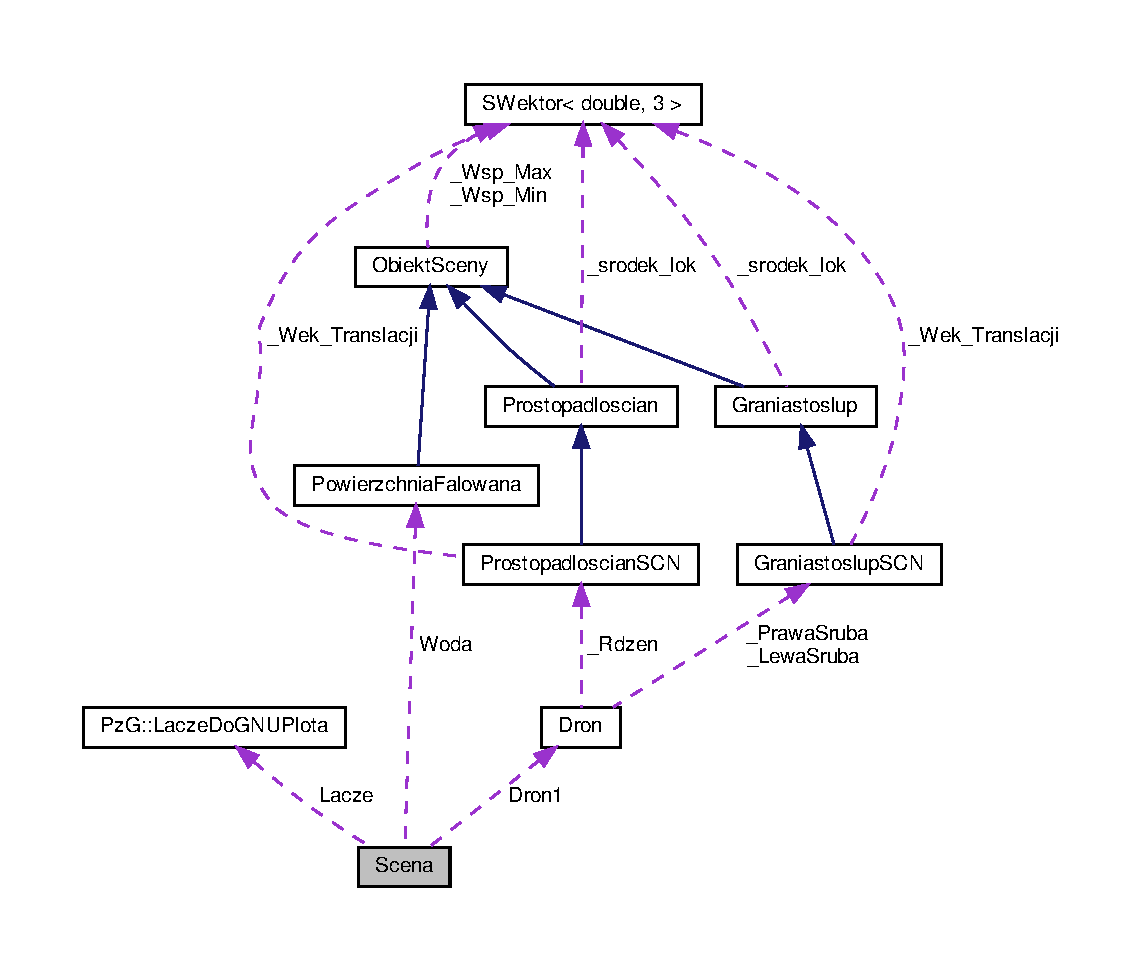
\includegraphics[width=350pt]{classScena__coll__graph}
\end{center}
\end{figure}
\subsection*{Metody publiczne}
\begin{DoxyCompactItemize}
\item 
\hyperlink{classDron}{Dron} \& \hyperlink{classScena_af1091cf596813b9bfd9988296098fb72}{Wez\+\_\+\+Drona1} ()
\begin{DoxyCompactList}\small\item\em Metoda umozliwia zewnetrzne odnoszenie sie do obiektu skladowego Dron1. \end{DoxyCompactList}\item 
bool \hyperlink{classScena_ab26c6debc2e4671ea62af02f42e2e16d}{Dodaj\+\_\+\+Powierzchnie} (const char $\ast$Nazwa\+Pliku)
\begin{DoxyCompactList}\small\item\em Metoda umozliwia dodanie do listy przeszkod elementu klasy \hyperlink{classPowierzchnia}{Powierzchnia}. \end{DoxyCompactList}\item 
bool \hyperlink{classScena_ab569c96c91809528437fa573ae21e9f7}{Dodaj\+\_\+\+Powierzchnie\+\_\+\+Falowana} (const char $\ast$Nazwa\+Pliku)
\begin{DoxyCompactList}\small\item\em Metoda umozliwia wczytanie powierzchni wody, klasy \hyperlink{classPowierzchniaFalowana}{Powierzchnia\+Falowana}. \end{DoxyCompactList}\item 
bool \hyperlink{classScena_a62a362fa6ff9abdfe81332546513ada8}{Dodaj\+\_\+\+Bryle} (const char $\ast$Nazwa\+Pliku)
\begin{DoxyCompactList}\small\item\em Metoda umozliwia dodanie do listy przeszkod elementu klasy \hyperlink{classProstopadloscian}{Prostopadloscian}. \end{DoxyCompactList}\item 
bool \hyperlink{classScena_a8c12fed91688fae5d233916590a4491d}{Dodaj\+\_\+\+Pret} (const char $\ast$Nazwa\+Pliku)
\begin{DoxyCompactList}\small\item\em Metoda umozliwia dodanie do listy przeszkod elementu klasy \hyperlink{classPret}{Pret}. \end{DoxyCompactList}\item 
void \hyperlink{classScena_a39bb68f2653e88942d49b52d0aa7da4d}{Wyczysc\+Liste} ()
\begin{DoxyCompactList}\small\item\em Metoda umozliwia zwolnienie pamieci listy. \end{DoxyCompactList}\item 
bool \hyperlink{classScena_ae4a2e4ac47a7d7183c3dd868d592a649}{Dodaj\+\_\+\+Drona} (\hyperlink{classDron}{Dron} \&Element, const char $\ast$Nazwa\+Pliku\+We\+Rdzen, const char $\ast$Nazwa\+Pliku\+We\+L\+Sruba, const char $\ast$Nazwa\+Pliku\+We\+P\+Sruba, const char $\ast$Nazwa\+Pliku\+Wy\+Rdzen, const char $\ast$Nazwa\+Pliku\+Wy\+L\+Sruba, const char $\ast$Nazwa\+Pliku\+Wy\+P\+Sruba)
\begin{DoxyCompactList}\small\item\em Metoda umozliwia wczytanie drona, klasy \hyperlink{classDron}{Dron} Metoda umozliwia wczytanie elementu sladowego dron, klasy \hyperlink{classDron}{Dron}, przypisujac mu odpowiednie pliki oraz przekazujac nazwy tych pliku do programu {\itshape gnuplot}. \end{DoxyCompactList}\item 
bool \hyperlink{classScena_a296cfc0d95b90f8818fc5a1bbd073929}{Inicjalizuj\+Scene} ()
\begin{DoxyCompactList}\small\item\em Metoda umozliwia inicjalizacje sceny. \end{DoxyCompactList}\item 
bool \hyperlink{classScena_a12ddfaedd1f01ba311e5b6ecba34840f}{Animowany\+\_\+\+Obrot\+\_\+\+Bryly} (\hyperlink{classDron}{Dron} \&Element, int kat)
\begin{DoxyCompactList}\small\item\em Metoda umozliwia animowany obrot drona. \end{DoxyCompactList}\item 
bool \hyperlink{classScena_acb95c285091570758e28c06dfa4f6d66}{Animowana\+\_\+\+Translacja\+\_\+\+Bryly} (\hyperlink{classDron}{Dron} \&Element, int kat\+\_\+z, unsigned int dlugosc)
\begin{DoxyCompactList}\small\item\em Metoda umozliwia animowany ruch drona. \end{DoxyCompactList}\end{DoxyCompactItemize}
\subsection*{Metody prywatne}
\begin{DoxyCompactItemize}
\item 
\hyperlink{classSWektor}{Wektor3D} \hyperlink{classScena_a624e04176f4f183d5c78604b66925534}{Oblicz\+Wektor\+Przesuniecia} (unsigned int dlugosc, int kat\+\_\+z, int kat\+\_\+orientacji) const
\begin{DoxyCompactList}\small\item\em Metoda umozliwia obliczenie wektora przesuniecia bryly. \end{DoxyCompactList}\item 
void \hyperlink{classScena_afa809376ae94fea3e939b9e354f882d3}{Rysuj\+\_\+\+Scene} ()
\begin{DoxyCompactList}\small\item\em Metoda umozliwia narysowanie obecnego stanu obiektow graficznych. \end{DoxyCompactList}\item 
bool \hyperlink{classScena_ad718f45ba059441502ae63688acb43ba}{Sprawdz\+Wynurzenie} (\hyperlink{classDron}{Dron} \&Element) const
\begin{DoxyCompactList}\small\item\em Realizuje sprawdzenie stopnia wynurzenia wskazanej ruchomej bryly. \end{DoxyCompactList}\end{DoxyCompactItemize}
\subsection*{Atrybuty prywatne}
\begin{DoxyCompactItemize}
\item 
\hyperlink{classPzG_1_1LaczeDoGNUPlota}{Pz\+G\+::\+Lacze\+Do\+G\+N\+U\+Plota} \hyperlink{classScena_ae8d7d121ba09af12c456a6dfe6da316b}{Lacze}
\begin{DoxyCompactList}\small\item\em Pole przechowuje zmienna umozliwiajaca przekazanie danych do programu {\itshape gnuplot}. \end{DoxyCompactList}\item 
\hyperlink{classDron}{Dron} \hyperlink{classScena_a98ad54358eeb2b6f1ea3c4b1c16c72b4}{Dron1}
\begin{DoxyCompactList}\small\item\em Pole przechowuje zmienna interpretujaca ruchomego drona. \end{DoxyCompactList}\item 
\hyperlink{classPowierzchniaFalowana}{Powierzchnia\+Falowana} \hyperlink{classScena_a6053a6a241f17e12f47717a73d0988d6}{Woda}
\begin{DoxyCompactList}\small\item\em Pole przechowuje zmienna interpretujaca powierzchnie wody. \end{DoxyCompactList}\item 
std\+::list$<$ \hyperlink{classObiektSceny}{Obiekt\+Sceny} $\ast$ $>$ \hyperlink{classScena_ad892638f354c23efb22296381aedd04f}{Lista}
\begin{DoxyCompactList}\small\item\em Pole przechowuje liste tworzonych dynamicznie przeszkód. \end{DoxyCompactList}\end{DoxyCompactItemize}


\subsection{Opis szczegółowy}
\hyperlink{classScena}{Scena} jako klasa zarzadzajaca obiektami graficznymi. 

Definicja klasy \hyperlink{classScena}{Scena}, sluzacej do zarzadzania graficznymi interpretacjami obiektow wykorzystywanych przez program. 

\subsection{Dokumentacja funkcji składowych}
\mbox{\Hypertarget{classScena_acb95c285091570758e28c06dfa4f6d66}\label{classScena_acb95c285091570758e28c06dfa4f6d66}} 
\index{Scena@{Scena}!Animowana\+\_\+\+Translacja\+\_\+\+Bryly@{Animowana\+\_\+\+Translacja\+\_\+\+Bryly}}
\index{Animowana\+\_\+\+Translacja\+\_\+\+Bryly@{Animowana\+\_\+\+Translacja\+\_\+\+Bryly}!Scena@{Scena}}
\subsubsection{\texorpdfstring{Animowana\+\_\+\+Translacja\+\_\+\+Bryly()}{Animowana\_Translacja\_Bryly()}}
{\footnotesize\ttfamily bool Scena\+::\+Animowana\+\_\+\+Translacja\+\_\+\+Bryly (\begin{DoxyParamCaption}\item[{\hyperlink{classDron}{Dron} \&}]{Element,  }\item[{int}]{kat\+\_\+z,  }\item[{unsigned int}]{dlugosc }\end{DoxyParamCaption})}



Metoda umozliwia animowany ruch drona. 

Metoda umozliwia animowany ruch drona z wykorzystaniem zdefiniowanych wartosci D\+O\+K\+L\+A\+D\+N\+O\+S\+C\+\_\+\+W\+E\+K\+T\+O\+R\+A\+\_\+\+O\+D\+S\+W\+I\+E\+Z\+A\+N\+IA (dlugosc wektora pojedynczej fazy ruchu) oraz C\+Z\+A\+S\+\_\+\+O\+D\+S\+W\+I\+E\+Z\+A\+N\+IA (czas miedzy kazda z faz ruchu, w ms). Przed kazda faza ruchu metoda sprawdza, czy nie spowodowalaby ona uderzenia o przeszkode lub nadmiernego wynurzenia. W pierwszym przypadku ruch zostaje przerwany, a w drugim ruch jest kontynuowany z zachowaniem stalej wysokosci drona. 
\begin{DoxyParams}[1]{Parametry}
\mbox{\tt in}  & {\em -\/} & Element -\/ referencja do przesuwanego obiektu \\
\hline
\mbox{\tt in}  & {\em -\/} & kat\+\_\+z -\/ kat wynurzenia/zanurzenia drona \\
\hline
\mbox{\tt in}  & {\em -\/} & dlugosc -\/ dlugosc zadanego ruchu \\
\hline
\end{DoxyParams}

\begin{DoxyRetVals}{Zwracane wartości}
{\em true} & -\/ ruch udalo sie wykonac poprawnie \\
\hline
{\em false} & -\/ nie udalo sie poprawnie wykonac operacji lub operacja spowodowalaby kolizje z dnem \\
\hline
\end{DoxyRetVals}
\mbox{\Hypertarget{classScena_a12ddfaedd1f01ba311e5b6ecba34840f}\label{classScena_a12ddfaedd1f01ba311e5b6ecba34840f}} 
\index{Scena@{Scena}!Animowany\+\_\+\+Obrot\+\_\+\+Bryly@{Animowany\+\_\+\+Obrot\+\_\+\+Bryly}}
\index{Animowany\+\_\+\+Obrot\+\_\+\+Bryly@{Animowany\+\_\+\+Obrot\+\_\+\+Bryly}!Scena@{Scena}}
\subsubsection{\texorpdfstring{Animowany\+\_\+\+Obrot\+\_\+\+Bryly()}{Animowany\_Obrot\_Bryly()}}
{\footnotesize\ttfamily bool Scena\+::\+Animowany\+\_\+\+Obrot\+\_\+\+Bryly (\begin{DoxyParamCaption}\item[{\hyperlink{classDron}{Dron} \&}]{Element,  }\item[{int}]{kat }\end{DoxyParamCaption})}



Metoda umozliwia animowany obrot drona. 

Metoda umozliwia animowany obrot drona z wykorzystaniem zdefiniowanych wartosci D\+O\+K\+L\+A\+D\+N\+O\+S\+C\+\_\+\+K\+A\+T\+A\+\_\+\+O\+D\+S\+W\+I\+E\+Z\+A\+N\+IA (kat pojedynczej fazy ruchu, w stopniach) oraz C\+Z\+A\+S\+\_\+\+O\+D\+S\+W\+I\+E\+Z\+A\+N\+IA (czas miedzy kazda z faz ruchu, w ms) 
\begin{DoxyParams}[1]{Parametry}
\mbox{\tt in}  & {\em -\/} & Element -\/ referencja do obracanego obiektu \\
\hline
\mbox{\tt in}  & {\em -\/} & kat -\/ kat o jaki dron ma sie obrocic \\
\hline
\end{DoxyParams}

\begin{DoxyRetVals}{Zwracane wartości}
{\em true} & -\/ obrot udalo sie wykonac poprawnie \\
\hline
{\em false} & -\/ nie udalo sie poprawnie wykonac operacji -\/ wystapil blad wyliczenia lub obrot spowodowalby kolizje z przeszkoda \\
\hline
\end{DoxyRetVals}
\mbox{\Hypertarget{classScena_a62a362fa6ff9abdfe81332546513ada8}\label{classScena_a62a362fa6ff9abdfe81332546513ada8}} 
\index{Scena@{Scena}!Dodaj\+\_\+\+Bryle@{Dodaj\+\_\+\+Bryle}}
\index{Dodaj\+\_\+\+Bryle@{Dodaj\+\_\+\+Bryle}!Scena@{Scena}}
\subsubsection{\texorpdfstring{Dodaj\+\_\+\+Bryle()}{Dodaj\_Bryle()}}
{\footnotesize\ttfamily bool Scena\+::\+Dodaj\+\_\+\+Bryle (\begin{DoxyParamCaption}\item[{const char $\ast$}]{Nazwa\+Pliku }\end{DoxyParamCaption})}



Metoda umozliwia dodanie do listy przeszkod elementu klasy \hyperlink{classProstopadloscian}{Prostopadloscian}. 

Metoda umozliwia dynamiczne nieruchomego elementu skladowego sceny, klasy \hyperlink{classProstopadloscian}{Prostopadloscian}, przypisujac mu odpowiedni plik oraz przekazujac nazwe tego pliku do programu {\itshape gnuplot}. Obiekt ten zostaje nastepnie zapamietany w liscie przeszkod. 
\begin{DoxyParams}[1]{Parametry}
\mbox{\tt in}  & {\em -\/} & Nazwa\+Pliku -\/ nazwa pliku z danymi lokalnymi dodawanej powierzchni \\
\hline
\end{DoxyParams}

\begin{DoxyRetVals}{Zwracane wartości}
{\em true} & -\/ element zostal wczytany poprawnie \\
\hline
{\em false} & -\/ nie udalo sie poprawnie wczytac elementu -\/ plik z danymi jest niepoprawny lub nie istnieje \\
\hline
\end{DoxyRetVals}
\mbox{\Hypertarget{classScena_ae4a2e4ac47a7d7183c3dd868d592a649}\label{classScena_ae4a2e4ac47a7d7183c3dd868d592a649}} 
\index{Scena@{Scena}!Dodaj\+\_\+\+Drona@{Dodaj\+\_\+\+Drona}}
\index{Dodaj\+\_\+\+Drona@{Dodaj\+\_\+\+Drona}!Scena@{Scena}}
\subsubsection{\texorpdfstring{Dodaj\+\_\+\+Drona()}{Dodaj\_Drona()}}
{\footnotesize\ttfamily bool Scena\+::\+Dodaj\+\_\+\+Drona (\begin{DoxyParamCaption}\item[{\hyperlink{classDron}{Dron} \&}]{Element,  }\item[{const char $\ast$}]{Nazwa\+Pliku\+We\+Rdzen,  }\item[{const char $\ast$}]{Nazwa\+Pliku\+We\+L\+Sruba,  }\item[{const char $\ast$}]{Nazwa\+Pliku\+We\+P\+Sruba,  }\item[{const char $\ast$}]{Nazwa\+Pliku\+Wy\+Rdzen,  }\item[{const char $\ast$}]{Nazwa\+Pliku\+Wy\+L\+Sruba,  }\item[{const char $\ast$}]{Nazwa\+Pliku\+Wy\+P\+Sruba }\end{DoxyParamCaption})}



Metoda umozliwia wczytanie drona, klasy \hyperlink{classDron}{Dron} Metoda umozliwia wczytanie elementu sladowego dron, klasy \hyperlink{classDron}{Dron}, przypisujac mu odpowiednie pliki oraz przekazujac nazwy tych pliku do programu {\itshape gnuplot}. 


\begin{DoxyParams}[1]{Parametry}
\mbox{\tt in}  & {\em -\/} & Element -\/ referencja do dodawanego drona \\
\hline
\mbox{\tt in}  & {\em -\/} & Nazwa\+Pliku\+We\+Rdzen -\/ nazwa pliku z danymi lokalnymi rdzenia drona \\
\hline
\mbox{\tt in}  & {\em -\/} & Nazwa\+Pliku\+Wy\+Rdzen -\/ nazwa pliku zapisu wspolrzedznych globalnych rdzenia drona \\
\hline
\mbox{\tt in}  & {\em -\/} & Nazwa\+Pliku\+We\+L\+Sruba -\/ nazwa pliku z danymi lokalnymi lewej sruby drona \\
\hline
\mbox{\tt in}  & {\em -\/} & Nazwa\+Pliku\+Wy\+L\+Sruba -\/ nazwa pliku zapisu wspolrzedznych globalnych lewej sruby drona \\
\hline
\mbox{\tt in}  & {\em -\/} & Nazwa\+Pliku\+We\+P\+Sruba -\/ nazwa pliku z danymi lokalnymi prawej sruby drona \\
\hline
\mbox{\tt in}  & {\em -\/} & Nazwa\+Pliku\+Wy\+P\+Sruba -\/ nazwa pliku zapisu wspolrzedznych globalnych prawej sruby drona \\
\hline
\end{DoxyParams}

\begin{DoxyRetVals}{Zwracane wartości}
{\em true} & -\/ element zostal wczytany poprawnie \\
\hline
{\em false} & -\/ nie udalo sie poprawnie wczytac elementu -\/ przynajmniej jeden plik z danymi jest niepoprawny lub nie istnieje \\
\hline
\end{DoxyRetVals}
\mbox{\Hypertarget{classScena_ab26c6debc2e4671ea62af02f42e2e16d}\label{classScena_ab26c6debc2e4671ea62af02f42e2e16d}} 
\index{Scena@{Scena}!Dodaj\+\_\+\+Powierzchnie@{Dodaj\+\_\+\+Powierzchnie}}
\index{Dodaj\+\_\+\+Powierzchnie@{Dodaj\+\_\+\+Powierzchnie}!Scena@{Scena}}
\subsubsection{\texorpdfstring{Dodaj\+\_\+\+Powierzchnie()}{Dodaj\_Powierzchnie()}}
{\footnotesize\ttfamily bool Scena\+::\+Dodaj\+\_\+\+Powierzchnie (\begin{DoxyParamCaption}\item[{const char $\ast$}]{Nazwa\+Pliku }\end{DoxyParamCaption})}



Metoda umozliwia dodanie do listy przeszkod elementu klasy \hyperlink{classPowierzchnia}{Powierzchnia}. 

Metoda umozliwia dynamiczne nieruchomego elementu skladowego sceny, klasy \hyperlink{classPowierzchnia}{Powierzchnia}, przypisujac mu odpowiedni plik oraz przekazujac nazwe tego pliku do programu {\itshape gnuplot}. Obiekt ten zostaje nastepnie zapamietany w liscie przeszkod. 
\begin{DoxyParams}[1]{Parametry}
\mbox{\tt in}  & {\em -\/} & Nazwa\+Pliku -\/ nazwa pliku z danymi lokalnymi dodawanej powierzchni \\
\hline
\end{DoxyParams}

\begin{DoxyRetVals}{Zwracane wartości}
{\em true} & -\/ element zostal wczytany poprawnie \\
\hline
{\em false} & -\/ nie udalo sie poprawnie wczytac elementu -\/ plik z danymi jest niepoprawny lub nie istnieje \\
\hline
\end{DoxyRetVals}
\mbox{\Hypertarget{classScena_ab569c96c91809528437fa573ae21e9f7}\label{classScena_ab569c96c91809528437fa573ae21e9f7}} 
\index{Scena@{Scena}!Dodaj\+\_\+\+Powierzchnie\+\_\+\+Falowana@{Dodaj\+\_\+\+Powierzchnie\+\_\+\+Falowana}}
\index{Dodaj\+\_\+\+Powierzchnie\+\_\+\+Falowana@{Dodaj\+\_\+\+Powierzchnie\+\_\+\+Falowana}!Scena@{Scena}}
\subsubsection{\texorpdfstring{Dodaj\+\_\+\+Powierzchnie\+\_\+\+Falowana()}{Dodaj\_Powierzchnie\_Falowana()}}
{\footnotesize\ttfamily bool Scena\+::\+Dodaj\+\_\+\+Powierzchnie\+\_\+\+Falowana (\begin{DoxyParamCaption}\item[{const char $\ast$}]{Nazwa\+Pliku }\end{DoxyParamCaption})}



Metoda umozliwia wczytanie powierzchni wody, klasy \hyperlink{classPowierzchniaFalowana}{Powierzchnia\+Falowana}. 

Metoda umozliwia wczytanie elementu sladowego Woda, klasy \hyperlink{classPowierzchniaFalowana}{Powierzchnia\+Falowana}, przypisujac mu odpowiedni plik oraz przekazujac nazwe tego pliku do programu {\itshape gnuplot} 
\begin{DoxyParams}[1]{Parametry}
\mbox{\tt in}  & {\em -\/} & Nazwa\+Pliku -\/ nazwa pliku z danymi lokalnymi dodawanej powierzchni \\
\hline
\end{DoxyParams}

\begin{DoxyRetVals}{Zwracane wartości}
{\em true} & -\/ element zostal wczytany poprawnie \\
\hline
{\em false} & -\/ nie udalo sie poprawnie wczytac elementu -\/ plik z danymi jest niepoprawny lub nie istnieje \\
\hline
\end{DoxyRetVals}
\mbox{\Hypertarget{classScena_a8c12fed91688fae5d233916590a4491d}\label{classScena_a8c12fed91688fae5d233916590a4491d}} 
\index{Scena@{Scena}!Dodaj\+\_\+\+Pret@{Dodaj\+\_\+\+Pret}}
\index{Dodaj\+\_\+\+Pret@{Dodaj\+\_\+\+Pret}!Scena@{Scena}}
\subsubsection{\texorpdfstring{Dodaj\+\_\+\+Pret()}{Dodaj\_Pret()}}
{\footnotesize\ttfamily bool Scena\+::\+Dodaj\+\_\+\+Pret (\begin{DoxyParamCaption}\item[{const char $\ast$}]{Nazwa\+Pliku }\end{DoxyParamCaption})}



Metoda umozliwia dodanie do listy przeszkod elementu klasy \hyperlink{classPret}{Pret}. 

Metoda umozliwia dynamiczne nieruchomego elementu skladowego sceny, klasy \hyperlink{classPret}{Pret}, przypisujac mu odpowiedni plik oraz przekazujac nazwe tego pliku do programu {\itshape gnuplot}. Obiekt ten zostaje nastepnie zapamietany w liscie przeszkod. 
\begin{DoxyParams}[1]{Parametry}
\mbox{\tt in}  & {\em -\/} & Nazwa\+Pliku -\/ nazwa pliku z danymi lokalnymi dodawanej powierzchni \\
\hline
\end{DoxyParams}

\begin{DoxyRetVals}{Zwracane wartości}
{\em true} & -\/ element zostal wczytany poprawnie \\
\hline
{\em false} & -\/ nie udalo sie poprawnie wczytac elementu -\/ plik z danymi jest niepoprawny lub nie istnieje \\
\hline
\end{DoxyRetVals}
\mbox{\Hypertarget{classScena_a296cfc0d95b90f8818fc5a1bbd073929}\label{classScena_a296cfc0d95b90f8818fc5a1bbd073929}} 
\index{Scena@{Scena}!Inicjalizuj\+Scene@{Inicjalizuj\+Scene}}
\index{Inicjalizuj\+Scene@{Inicjalizuj\+Scene}!Scena@{Scena}}
\subsubsection{\texorpdfstring{Inicjalizuj\+Scene()}{InicjalizujScene()}}
{\footnotesize\ttfamily bool Scena\+::\+Inicjalizuj\+Scene (\begin{DoxyParamCaption}{ }\end{DoxyParamCaption})}



Metoda umozliwia inicjalizacje sceny. 

Metoda umozliwia inicjalizacje sceny, wczytujac elementy okreslone w polach klasy, dodajac do listy przekszód po jednym przykladzie kazdej przeszkody oraz przekazujac programowi {\itshape gnuplot} nazwy plikow, na podstawie ktorych rysowana bedzie scena. W przypadku poprawnej inicjalizacji program {\itshape gnuplot} rozpoczyna prace od narysowania graficznej interpretacji poczatkowego stanu sceny.


\begin{DoxyRetVals}{Zwracane wartości}
{\em true} & -\/ inicjalizacja przebiegla pomyslnie \\
\hline
{\em false} & -\/ nie udalo sie poprawnie wczytac elementow sceny \\
\hline
\end{DoxyRetVals}
\mbox{\Hypertarget{classScena_a624e04176f4f183d5c78604b66925534}\label{classScena_a624e04176f4f183d5c78604b66925534}} 
\index{Scena@{Scena}!Oblicz\+Wektor\+Przesuniecia@{Oblicz\+Wektor\+Przesuniecia}}
\index{Oblicz\+Wektor\+Przesuniecia@{Oblicz\+Wektor\+Przesuniecia}!Scena@{Scena}}
\subsubsection{\texorpdfstring{Oblicz\+Wektor\+Przesuniecia()}{ObliczWektorPrzesuniecia()}}
{\footnotesize\ttfamily \hyperlink{classSWektor}{Wektor3D} Scena\+::\+Oblicz\+Wektor\+Przesuniecia (\begin{DoxyParamCaption}\item[{unsigned int}]{dlugosc,  }\item[{int}]{kat\+\_\+z,  }\item[{int}]{kat\+\_\+orientacji }\end{DoxyParamCaption}) const\hspace{0.3cm}{\ttfamily [private]}}



Metoda umozliwia obliczenie wektora przesuniecia bryly. 

Metoda umozliwia obliczenie wektora przesuniecia bryly, uwzgledniajac jej obecny kat orientacji oraz wskazany kat wynurzenia/zanurzenia


\begin{DoxyParams}[1]{Parametry}
\mbox{\tt in}  & {\em dlugosc} & -\/ zadana dlugosc wektora przesuniecia \\
\hline
\mbox{\tt in}  & {\em kat\+\_\+z} & -\/ zadana kat wynurzenia/zanurzenia \\
\hline
\mbox{\tt in}  & {\em kat\+\_\+orientacji} & -\/ aktualny kat orientacji bryly wokol osi OZ \\
\hline
\end{DoxyParams}

\begin{DoxyRetVals}{Zwracane wartości}
{\em Wektor3D} & -\/ okreslajacy zmiane polozenia \\
\hline
\end{DoxyRetVals}
\mbox{\Hypertarget{classScena_afa809376ae94fea3e939b9e354f882d3}\label{classScena_afa809376ae94fea3e939b9e354f882d3}} 
\index{Scena@{Scena}!Rysuj\+\_\+\+Scene@{Rysuj\+\_\+\+Scene}}
\index{Rysuj\+\_\+\+Scene@{Rysuj\+\_\+\+Scene}!Scena@{Scena}}
\subsubsection{\texorpdfstring{Rysuj\+\_\+\+Scene()}{Rysuj\_Scene()}}
{\footnotesize\ttfamily void Scena\+::\+Rysuj\+\_\+\+Scene (\begin{DoxyParamCaption}{ }\end{DoxyParamCaption})\hspace{0.3cm}{\ttfamily [inline]}, {\ttfamily [private]}}



Metoda umozliwia narysowanie obecnego stanu obiektow graficznych. 

Metoda umozliwia narysowanie obecnego stanu obiektow graficznych za pomoca metody \hyperlink{classPzG_1_1LaczeDoGNUPlota_a065f5b8402737cc62b0ad4f66d028335}{Pz\+G\+::\+Lacze\+Do\+G\+N\+U\+Plota\+::\+Rysuj} wykorzystujacej w tym celu dane przekazane do programu {\itshape gnuplot} \mbox{\Hypertarget{classScena_ad718f45ba059441502ae63688acb43ba}\label{classScena_ad718f45ba059441502ae63688acb43ba}} 
\index{Scena@{Scena}!Sprawdz\+Wynurzenie@{Sprawdz\+Wynurzenie}}
\index{Sprawdz\+Wynurzenie@{Sprawdz\+Wynurzenie}!Scena@{Scena}}
\subsubsection{\texorpdfstring{Sprawdz\+Wynurzenie()}{SprawdzWynurzenie()}}
{\footnotesize\ttfamily bool Scena\+::\+Sprawdz\+Wynurzenie (\begin{DoxyParamCaption}\item[{\hyperlink{classDron}{Dron} \&}]{Element }\end{DoxyParamCaption}) const\hspace{0.3cm}{\ttfamily [private]}}



Realizuje sprawdzenie stopnia wynurzenia wskazanej ruchomej bryly. 

Realizuje sprawdzenie stopnia wynurzenia wskazanej ruchomej bryly poprzez porownanie wspolrzednych skrajnych bryly po translacji oraz powierzchni falowanej oznaczajacej wode

\begin{DoxyPrecond}{Warunek wstępny}
Obiekty musza zostac wczesniej poprawnie zainicjalizowane 

Sprawdzenie wynurzenia powinno wystapic po zarejestrowaniu bezkolizyjnej translacji 
\end{DoxyPrecond}

\begin{DoxyParams}[1]{Parametry}
\mbox{\tt in}  & {\em \hyperlink{classDron}{Dron}} & -\/ referencja do drona, umozliwiajaca sprawdzenie jego polozenia \\
\hline
\end{DoxyParams}

\begin{DoxyRetVals}{Zwracane wartości}
{\em true} & -\/ zadany ruch spowodowalby wydostanie sie ponad maksymalne wynurzenie \\
\hline
{\em false} & -\/ zadany ruch jest dopuszczalny \\
\hline
\end{DoxyRetVals}
\mbox{\Hypertarget{classScena_af1091cf596813b9bfd9988296098fb72}\label{classScena_af1091cf596813b9bfd9988296098fb72}} 
\index{Scena@{Scena}!Wez\+\_\+\+Drona1@{Wez\+\_\+\+Drona1}}
\index{Wez\+\_\+\+Drona1@{Wez\+\_\+\+Drona1}!Scena@{Scena}}
\subsubsection{\texorpdfstring{Wez\+\_\+\+Drona1()}{Wez\_Drona1()}}
{\footnotesize\ttfamily \hyperlink{classDron}{Dron}\& Scena\+::\+Wez\+\_\+\+Drona1 (\begin{DoxyParamCaption}{ }\end{DoxyParamCaption})\hspace{0.3cm}{\ttfamily [inline]}}



Metoda umozliwia zewnetrzne odnoszenie sie do obiektu skladowego Dron1. 

Metoda umozliwia zewnetrzne odnoszenie sie do obiektu skladowego Dron1 
\begin{DoxyRetVals}{Zwracane wartości}
{\em Dron1} & -\/ referencja do obiektu Dron1 klasy \hyperlink{classDron}{Dron} \\
\hline
\end{DoxyRetVals}
\mbox{\Hypertarget{classScena_a39bb68f2653e88942d49b52d0aa7da4d}\label{classScena_a39bb68f2653e88942d49b52d0aa7da4d}} 
\index{Scena@{Scena}!Wyczysc\+Liste@{Wyczysc\+Liste}}
\index{Wyczysc\+Liste@{Wyczysc\+Liste}!Scena@{Scena}}
\subsubsection{\texorpdfstring{Wyczysc\+Liste()}{WyczyscListe()}}
{\footnotesize\ttfamily void Scena\+::\+Wyczysc\+Liste (\begin{DoxyParamCaption}{ }\end{DoxyParamCaption})\hspace{0.3cm}{\ttfamily [inline]}}



Metoda umozliwia zwolnienie pamieci listy. 

Metoda umozliwia zwolnienie pamieci listy, usuwajac dynamicznie po kolei wszystkie jej obiekty, wykorzystujac petle zakresu 

\subsection{Dokumentacja atrybutów składowych}
\mbox{\Hypertarget{classScena_a98ad54358eeb2b6f1ea3c4b1c16c72b4}\label{classScena_a98ad54358eeb2b6f1ea3c4b1c16c72b4}} 
\index{Scena@{Scena}!Dron1@{Dron1}}
\index{Dron1@{Dron1}!Scena@{Scena}}
\subsubsection{\texorpdfstring{Dron1}{Dron1}}
{\footnotesize\ttfamily \hyperlink{classDron}{Dron} Scena\+::\+Dron1\hspace{0.3cm}{\ttfamily [private]}}



Pole przechowuje zmienna interpretujaca ruchomego drona. 

Pole przechowuje zmienna interpretujaca ruchomego drona za pomoca klasy \hyperlink{classDron}{Dron} \mbox{\Hypertarget{classScena_ae8d7d121ba09af12c456a6dfe6da316b}\label{classScena_ae8d7d121ba09af12c456a6dfe6da316b}} 
\index{Scena@{Scena}!Lacze@{Lacze}}
\index{Lacze@{Lacze}!Scena@{Scena}}
\subsubsection{\texorpdfstring{Lacze}{Lacze}}
{\footnotesize\ttfamily \hyperlink{classPzG_1_1LaczeDoGNUPlota}{Pz\+G\+::\+Lacze\+Do\+G\+N\+U\+Plota} Scena\+::\+Lacze\hspace{0.3cm}{\ttfamily [private]}}



Pole przechowuje zmienna umozliwiajaca przekazanie danych do programu {\itshape gnuplot}. 

Pole przechowuje zmienna umozliwiajaca przekazywanie danych rysunku do programu {\itshape gnuplot} za pomoca klasy \hyperlink{classPzG_1_1LaczeDoGNUPlota}{Pz\+G\+::\+Lacze\+Do\+G\+N\+U\+Plota} \mbox{\Hypertarget{classScena_ad892638f354c23efb22296381aedd04f}\label{classScena_ad892638f354c23efb22296381aedd04f}} 
\index{Scena@{Scena}!Lista@{Lista}}
\index{Lista@{Lista}!Scena@{Scena}}
\subsubsection{\texorpdfstring{Lista}{Lista}}
{\footnotesize\ttfamily std\+::list$<$\hyperlink{classObiektSceny}{Obiekt\+Sceny}$\ast$$>$ Scena\+::\+Lista\hspace{0.3cm}{\ttfamily [private]}}



Pole przechowuje liste tworzonych dynamicznie przeszkód. 

Pole przechowuje liste tworzonych dynamicznie przeszkod za pomoca obiektu typu std\+::list Lista okreslona jest dla klasy \hyperlink{classObiektSceny}{Obiekt\+Sceny} bedacej klasa bazowa kazdego rodzaju przeszkody -\/ podczas dynamicznego dodawania kolejnych obiektow nastepuje rzutowanie w gore na klase bazowa \mbox{\Hypertarget{classScena_a6053a6a241f17e12f47717a73d0988d6}\label{classScena_a6053a6a241f17e12f47717a73d0988d6}} 
\index{Scena@{Scena}!Woda@{Woda}}
\index{Woda@{Woda}!Scena@{Scena}}
\subsubsection{\texorpdfstring{Woda}{Woda}}
{\footnotesize\ttfamily \hyperlink{classPowierzchniaFalowana}{Powierzchnia\+Falowana} Scena\+::\+Woda\hspace{0.3cm}{\ttfamily [private]}}



Pole przechowuje zmienna interpretujaca powierzchnie wody. 

Pole przechowuje zmienna interpretujaca powierzchnie wody za pomoca klasy \hyperlink{classPowierzchniaFalowana}{Powierzchnia\+Falowana} 

Dokumentacja dla tej klasy została wygenerowana z plików\+:\begin{DoxyCompactItemize}
\item 
inc/\hyperlink{Scena_8hh}{Scena.\+hh}\item 
src/\hyperlink{Scena_8cpp}{Scena.\+cpp}\end{DoxyCompactItemize}

\hypertarget{classSMacierz}{}\section{Dokumentacja szablonu klasy S\+Macierz$<$ Typ, Wymiar $>$}
\label{classSMacierz}\index{S\+Macierz$<$ Typ, Wymiar $>$@{S\+Macierz$<$ Typ, Wymiar $>$}}


Klasa modeluje pojęcie macierzy kwadratowej.  




{\ttfamily \#include $<$S\+Macierz.\+hh$>$}

\subsection*{Metody publiczne}
\begin{DoxyCompactItemize}
\item 
\mbox{\Hypertarget{classSMacierz_a7fa53b3a5b5b07e82493dc55447f5546}\label{classSMacierz_a7fa53b3a5b5b07e82493dc55447f5546}} 
const \hyperlink{classSWektor}{S\+Wektor}$<$ Typ, Wymiar $>$ \& {\bfseries operator\mbox{[}$\,$\mbox{]}} (unsigned int Kol) const
\item 
\mbox{\Hypertarget{classSMacierz_afc5e3fea0f930ea3ed722551c5c7e553}\label{classSMacierz_afc5e3fea0f930ea3ed722551c5c7e553}} 
\hyperlink{classSWektor}{S\+Wektor}$<$ Typ, Wymiar $>$ \& {\bfseries operator\mbox{[}$\,$\mbox{]}} (unsigned int Kol)
\item 
\mbox{\Hypertarget{classSMacierz_a3176386344a6b9be84922c736f04e7d6}\label{classSMacierz_a3176386344a6b9be84922c736f04e7d6}} 
const Typ {\bfseries operator()} (unsigned int Wie, unsigned int Kol) const
\item 
\mbox{\Hypertarget{classSMacierz_a799597af607b21870e608fe4afe6c4ed}\label{classSMacierz_a799597af607b21870e608fe4afe6c4ed}} 
Typ \& {\bfseries operator()} (unsigned int Wie, unsigned int Kol)
\item 
\hyperlink{classSWektor}{S\+Wektor}$<$ Typ, Wymiar $>$ \hyperlink{classSMacierz_ae72c507f32c5ce3db5ded6acacc64bc3}{operator$\ast$} (const \hyperlink{classSWektor}{S\+Wektor}$<$ Typ, Wymiar $>$ \&Wek) const
\item 
const Typ \hyperlink{classSMacierz_a1445d4e0c95d303e28d2f89e9751d77d}{Wyznacznik} () const
\item 
void \hyperlink{classSMacierz_a3dd718281652814e45a5fe17f2c33b05}{operator=} (const \hyperlink{classSMacierz}{S\+Macierz}$<$ Typ, Wymiar $>$ \&Mac)
\end{DoxyCompactItemize}
\subsection*{Metody prywatne}
\begin{DoxyCompactItemize}
\item 
void \hyperlink{classSMacierz_afee8329b07e345879eead08f3a316f62}{Zamiana\+\_\+kolumn\+\_\+w\+\_\+macierzy} (unsigned int indeks1, unsigned int indeks2)
\item 
int \hyperlink{classSMacierz_aceb9638a718d4e5e0a03a020b041aa0d}{Zamiana\+\_\+z\+\_\+elementem\+\_\+niezerowym\+\_\+i\+\_\+zmiana\+\_\+mnoznika} (unsigned int indeks\+\_\+kolumny)
\item 
bool \hyperlink{classSMacierz_aca41f9c5eaf53fdb6ddb5f065f816fcd}{Sprowadz\+\_\+do\+\_\+trojkatnej} (int \&mnoznik\+\_\+wyznacznika)
\item 
const Typ \hyperlink{classSMacierz_a89430b42ebd5e4b6a5bd65b91d2124ca}{Wyznacznik\+\_\+\+Oblicz} ()
\end{DoxyCompactItemize}
\subsection*{Atrybuty prywatne}
\begin{DoxyCompactItemize}
\item 
\mbox{\Hypertarget{classSMacierz_aba0891504ff93e4d1678867e2d787b1c}\label{classSMacierz_aba0891504ff93e4d1678867e2d787b1c}} 
\hyperlink{classSWektor}{S\+Wektor}$<$ Typ, Wymiar $>$ {\bfseries \+\_\+\+Kolumna} \mbox{[}Wymiar\mbox{]}
\end{DoxyCompactItemize}


\subsection{Opis szczegółowy}
\subsubsection*{template$<$typename Typ, int Wymiar$>$\newline
class S\+Macierz$<$ Typ, Wymiar $>$}

Klasa modeluje pojęcie macierzy kwadratowej. 

Klasa modeluje pojęcie macierzy jako jednowymiarowej tablicy wektorów o wielkości \char`\"{}\+Wymiar\char`\"{}. Zawiera metody umożliwiające pobranie wartosci wybranego pola z wybranego wektora tablicy klasy, czy też jego modyfikację. Ponadto umożliwia wykonanie mnożenia macierzy przez wektor, wyliczenie wyznacznika, transpozycję macierzy oraz podstawienie jednej macierzy do drugiej. 

\subsection{Dokumentacja funkcji składowych}
\mbox{\Hypertarget{classSMacierz_ae72c507f32c5ce3db5ded6acacc64bc3}\label{classSMacierz_ae72c507f32c5ce3db5ded6acacc64bc3}} 
\index{S\+Macierz@{S\+Macierz}!operator$\ast$@{operator$\ast$}}
\index{operator$\ast$@{operator$\ast$}!S\+Macierz@{S\+Macierz}}
\subsubsection{\texorpdfstring{operator$\ast$()}{operator*()}}
{\footnotesize\ttfamily template$<$typename Typ , int Wymiar$>$ \\
\hyperlink{classSWektor}{S\+Wektor}$<$ Typ, Wymiar $>$ \hyperlink{classSMacierz}{S\+Macierz}$<$ Typ, Wymiar $>$\+::operator$\ast$ (\begin{DoxyParamCaption}\item[{const \hyperlink{classSWektor}{S\+Wektor}$<$ Typ, Wymiar $>$ \&}]{Wek }\end{DoxyParamCaption}) const}

Mnozenie stalej macierzy wywolania przez staly wektor wywolania Argumenty\+: Wek -\/ referencja do stalego wektora -\/ klasy \hyperlink{classSWektor}{S\+Wektor} Argument domyslny -\/ staly obiekt klasy \hyperlink{classSMacierz}{S\+Macierz} Zwraca\+: wynik -\/ wektor bedacy wynikiem operacji mnozenia \mbox{\Hypertarget{classSMacierz_a3dd718281652814e45a5fe17f2c33b05}\label{classSMacierz_a3dd718281652814e45a5fe17f2c33b05}} 
\index{S\+Macierz@{S\+Macierz}!operator=@{operator=}}
\index{operator=@{operator=}!S\+Macierz@{S\+Macierz}}
\subsubsection{\texorpdfstring{operator=()}{operator=()}}
{\footnotesize\ttfamily template$<$typename Typ , int Wymiar$>$ \\
void \hyperlink{classSMacierz}{S\+Macierz}$<$ Typ, Wymiar $>$\+::operator= (\begin{DoxyParamCaption}\item[{const \hyperlink{classSMacierz}{S\+Macierz}$<$ Typ, Wymiar $>$ \&}]{Mac }\end{DoxyParamCaption})}

Przypisanie wartości elementów stalej macierzy argumentu do wartości elementów macierzy wywołania Argumenty\+: Mac -\/ referencja do stalej macierzy -\/ obiektu klasy \hyperlink{classSMacierz}{S\+Macierz} Argument domyslny -\/ modyfikowalny obiekt klasy \hyperlink{classSMacierz}{S\+Macierz} \mbox{\Hypertarget{classSMacierz_aca41f9c5eaf53fdb6ddb5f065f816fcd}\label{classSMacierz_aca41f9c5eaf53fdb6ddb5f065f816fcd}} 
\index{S\+Macierz@{S\+Macierz}!Sprowadz\+\_\+do\+\_\+trojkatnej@{Sprowadz\+\_\+do\+\_\+trojkatnej}}
\index{Sprowadz\+\_\+do\+\_\+trojkatnej@{Sprowadz\+\_\+do\+\_\+trojkatnej}!S\+Macierz@{S\+Macierz}}
\subsubsection{\texorpdfstring{Sprowadz\+\_\+do\+\_\+trojkatnej()}{Sprowadz\_do\_trojkatnej()}}
{\footnotesize\ttfamily template$<$typename Typ , int Wymiar$>$ \\
bool \hyperlink{classSMacierz}{S\+Macierz}$<$ Typ, Wymiar $>$\+::Sprowadz\+\_\+do\+\_\+trojkatnej (\begin{DoxyParamCaption}\item[{int \&}]{mnoznik }\end{DoxyParamCaption})\hspace{0.3cm}{\ttfamily [private]}}

Realizuje sprowadzenie macierzy wywolania do macierzy trojkatnej Argumenty\+: Argumenty domyślny -\/ modyfikowalny obiekt klasy \hyperlink{classSMacierz}{S\+Macierz} mnoznik -\/ referencja do obiektu int, ktory ulega zmianie w zaleznosci od ilosci wykonania operacji zamiany dwoch kolumn miejscami. Obiekt ten moze przyjac wartosc 1, -\/1 lub 0. Zwraca\+: false -\/ nie udalo sie sprowadzic do macierzy trojkatnej true -\/ udalo sie sprowadzic do macierzy trojkatnej \mbox{\Hypertarget{classSMacierz_a1445d4e0c95d303e28d2f89e9751d77d}\label{classSMacierz_a1445d4e0c95d303e28d2f89e9751d77d}} 
\index{S\+Macierz@{S\+Macierz}!Wyznacznik@{Wyznacznik}}
\index{Wyznacznik@{Wyznacznik}!S\+Macierz@{S\+Macierz}}
\subsubsection{\texorpdfstring{Wyznacznik()}{Wyznacznik()}}
{\footnotesize\ttfamily template$<$typename Typ , int Wymiar$>$ \\
const Typ \hyperlink{classSMacierz}{S\+Macierz}$<$ Typ, Wymiar $>$\+::Wyznacznik (\begin{DoxyParamCaption}{ }\end{DoxyParamCaption}) const}

Podaje wartosc wyznacznika macierzy wywolania Argumenty\+: Argumenty domyślny -\/ staly obiekt klasy \hyperlink{classSMacierz}{S\+Macierz} Zwraca\+: Wyliczona wartosc wyznacznika \mbox{\Hypertarget{classSMacierz_a89430b42ebd5e4b6a5bd65b91d2124ca}\label{classSMacierz_a89430b42ebd5e4b6a5bd65b91d2124ca}} 
\index{S\+Macierz@{S\+Macierz}!Wyznacznik\+\_\+\+Oblicz@{Wyznacznik\+\_\+\+Oblicz}}
\index{Wyznacznik\+\_\+\+Oblicz@{Wyznacznik\+\_\+\+Oblicz}!S\+Macierz@{S\+Macierz}}
\subsubsection{\texorpdfstring{Wyznacznik\+\_\+\+Oblicz()}{Wyznacznik\_Oblicz()}}
{\footnotesize\ttfamily template$<$typename Typ , int Wymiar$>$ \\
const Typ \hyperlink{classSMacierz}{S\+Macierz}$<$ Typ, Wymiar $>$\+::Wyznacznik\+\_\+\+Oblicz (\begin{DoxyParamCaption}{ }\end{DoxyParamCaption})\hspace{0.3cm}{\ttfamily [private]}}

Realizuje obliczenie wartosci wyznacznika macierzy wywolania Argumenty\+: Argumenty domyślny -\/ modyfikowalny obiekt klasy \hyperlink{classSMacierz}{S\+Macierz} Zwraca\+: wartosc -\/ wyliczona wartosc wynzacznika macierzy \mbox{\Hypertarget{classSMacierz_afee8329b07e345879eead08f3a316f62}\label{classSMacierz_afee8329b07e345879eead08f3a316f62}} 
\index{S\+Macierz@{S\+Macierz}!Zamiana\+\_\+kolumn\+\_\+w\+\_\+macierzy@{Zamiana\+\_\+kolumn\+\_\+w\+\_\+macierzy}}
\index{Zamiana\+\_\+kolumn\+\_\+w\+\_\+macierzy@{Zamiana\+\_\+kolumn\+\_\+w\+\_\+macierzy}!S\+Macierz@{S\+Macierz}}
\subsubsection{\texorpdfstring{Zamiana\+\_\+kolumn\+\_\+w\+\_\+macierzy()}{Zamiana\_kolumn\_w\_macierzy()}}
{\footnotesize\ttfamily template$<$typename Typ , int Wymiar$>$ \\
void \hyperlink{classSMacierz}{S\+Macierz}$<$ Typ, Wymiar $>$\+::Zamiana\+\_\+kolumn\+\_\+w\+\_\+macierzy (\begin{DoxyParamCaption}\item[{unsigned int}]{indeks1,  }\item[{unsigned int}]{indeks2 }\end{DoxyParamCaption})\hspace{0.3cm}{\ttfamily [private]}}

Zamiana miejscami dwóch wybranych kolumn w macierzy wywołania Argumenty\+: Argumenty domyślny -\/ modyfikowalny obiekt klasy \hyperlink{classSMacierz}{S\+Macierz} indeks1, indeks2 -\/ indeksy wybranych kolumn do zamiany \mbox{\Hypertarget{classSMacierz_aceb9638a718d4e5e0a03a020b041aa0d}\label{classSMacierz_aceb9638a718d4e5e0a03a020b041aa0d}} 
\index{S\+Macierz@{S\+Macierz}!Zamiana\+\_\+z\+\_\+elementem\+\_\+niezerowym\+\_\+i\+\_\+zmiana\+\_\+mnoznika@{Zamiana\+\_\+z\+\_\+elementem\+\_\+niezerowym\+\_\+i\+\_\+zmiana\+\_\+mnoznika}}
\index{Zamiana\+\_\+z\+\_\+elementem\+\_\+niezerowym\+\_\+i\+\_\+zmiana\+\_\+mnoznika@{Zamiana\+\_\+z\+\_\+elementem\+\_\+niezerowym\+\_\+i\+\_\+zmiana\+\_\+mnoznika}!S\+Macierz@{S\+Macierz}}
\subsubsection{\texorpdfstring{Zamiana\+\_\+z\+\_\+elementem\+\_\+niezerowym\+\_\+i\+\_\+zmiana\+\_\+mnoznika()}{Zamiana\_z\_elementem\_niezerowym\_i\_zmiana\_mnoznika()}}
{\footnotesize\ttfamily template$<$typename Typ , int Wymiar$>$ \\
int \hyperlink{classSMacierz}{S\+Macierz}$<$ Typ, Wymiar $>$\+::Zamiana\+\_\+z\+\_\+elementem\+\_\+niezerowym\+\_\+i\+\_\+zmiana\+\_\+mnoznika (\begin{DoxyParamCaption}\item[{unsigned int}]{indeks\+\_\+zera }\end{DoxyParamCaption})\hspace{0.3cm}{\ttfamily [private]}}

Realizuje przegladanie wybranego wiersza macierzy w celu odnalezienia kolumny z elementem niezerowym, a nastepnie zamiane kolumn. Argumenty\+: Argumenty domyślny -\/ modyfikowalny obiekt klasy \hyperlink{classSMacierz}{S\+Macierz} indeks\+\_\+zera -\/ okresla wiersz, ktory przeszukujemy oraz kolumne poprzedzajaca ta, od ktorej zaczynamy przeszukiwanie Zwraca\+: 0 -\/ nie udalo sie odnalezc elementu niezerowego -\/1 -\/ udalo sie odnalezc element niezerowy -\/ mnoznik wyznacznika zmienia znak na przeciwny 

Dokumentacja dla tej klasy została wygenerowana z pliku\+:\begin{DoxyCompactItemize}
\item 
inc/\hyperlink{SMacierz_8hh}{S\+Macierz.\+hh}\end{DoxyCompactItemize}

\hypertarget{classSWektor}{}\section{Dokumentacja szablonu klasy S\+Wektor$<$ Typ, Wymiar $>$}
\label{classSWektor}\index{S\+Wektor$<$ Typ, Wymiar $>$@{S\+Wektor$<$ Typ, Wymiar $>$}}


Klasa modeluje pojecie wektora.  




{\ttfamily \#include $<$S\+Wektor.\+hh$>$}



Diagram współpracy dla S\+Wektor$<$ Typ, Wymiar $>$\+:\nopagebreak
\begin{figure}[H]
\begin{center}
\leavevmode
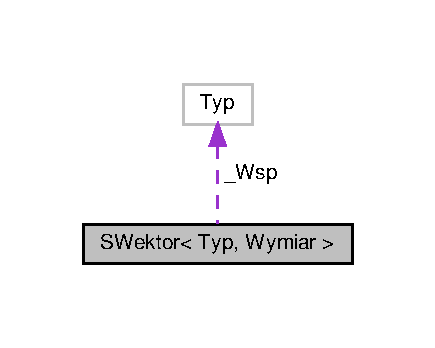
\includegraphics[width=209pt]{classSWektor__coll__graph}
\end{center}
\end{figure}
\subsection*{Metody publiczne}
\begin{DoxyCompactItemize}
\item 
\mbox{\Hypertarget{classSWektor_a30dfcfc08257aeeb41bc96c32704f431}\label{classSWektor_a30dfcfc08257aeeb41bc96c32704f431}} 
const Typ {\bfseries operator\mbox{[}$\,$\mbox{]}} (unsigned int indeks) const
\item 
\mbox{\Hypertarget{classSWektor_a39a12c33739ea481b627f2eaea3c4658}\label{classSWektor_a39a12c33739ea481b627f2eaea3c4658}} 
Typ \& {\bfseries operator\mbox{[}$\,$\mbox{]}} (unsigned int indeks)
\item 
\hyperlink{classSWektor}{S\+Wektor}$<$ Typ, Wymiar $>$ \hyperlink{classSWektor_ad6edecba069a5fa43685eae4de64126a}{operator-\/} (const \hyperlink{classSWektor}{S\+Wektor}$<$ Typ, Wymiar $>$ \&wek) const
\item 
\hyperlink{classSWektor}{S\+Wektor}$<$ Typ, Wymiar $>$ \hyperlink{classSWektor_a088f294837df1f61cb577c26646ba76a}{operator+} (const \hyperlink{classSWektor}{S\+Wektor}$<$ Typ, Wymiar $>$ \&wek) const
\item 
Typ \hyperlink{classSWektor_a216a89c4fa018c75ae11af6e0cf26b23}{operator$\ast$} (const \hyperlink{classSWektor}{S\+Wektor}$<$ Typ, Wymiar $>$ \&wek) const
\item 
\hyperlink{classSWektor}{S\+Wektor}$<$ Typ, Wymiar $>$ \hyperlink{classSWektor_a58efd989f2647747bcc68e9650e38647}{operator$\ast$} (Typ liczba) const
\item 
\hyperlink{classSWektor}{S\+Wektor}$<$ Typ, Wymiar $>$ \hyperlink{classSWektor_a80fde5a5dca1d5b261bda6c4da826134}{operator/} (Typ liczba) const
\item 
void \hyperlink{classSWektor_a03255e5b60c400972aad2a56f06832c4}{operator=} (const \hyperlink{classSWektor}{S\+Wektor}$<$ Typ, Wymiar $>$ \&wek)
\end{DoxyCompactItemize}
\subsection*{Atrybuty prywatne}
\begin{DoxyCompactItemize}
\item 
\mbox{\Hypertarget{classSWektor_a5b623317072fcf2d05ece0e30a819c81}\label{classSWektor_a5b623317072fcf2d05ece0e30a819c81}} 
Typ {\bfseries \+\_\+\+Wsp} \mbox{[}Wymiar\mbox{]}
\end{DoxyCompactItemize}


\subsection{Opis szczegółowy}
\subsubsection*{template$<$typename Typ, int Wymiar$>$\newline
class S\+Wektor$<$ Typ, Wymiar $>$}

Klasa modeluje pojecie wektora. 

Klasa modeluje pojęcie wektora jako jednowymiarowej tablicy elementów double, o rozmiarze R\+O\+Z\+M\+I\+AR. Zawiera metody umożliwiające pobranie wartosci wybranego pola tablicy klasy, czy też jego modyfikację. Ponadto umożliwia wykonywanie działań arytmetycznych na wektorach, mnożenie i dzielenie wektora przez liczbę typu double, podanie długości wektora oraz przypisanie jednego wektora do drugiego. 

\subsection{Dokumentacja funkcji składowych}
\mbox{\Hypertarget{classSWektor_a216a89c4fa018c75ae11af6e0cf26b23}\label{classSWektor_a216a89c4fa018c75ae11af6e0cf26b23}} 
\index{S\+Wektor@{S\+Wektor}!operator$\ast$@{operator$\ast$}}
\index{operator$\ast$@{operator$\ast$}!S\+Wektor@{S\+Wektor}}
\subsubsection{\texorpdfstring{operator$\ast$()}{operator*()}\hspace{0.1cm}{\footnotesize\ttfamily [1/2]}}
{\footnotesize\ttfamily template$<$typename Typ, int Wymiar$>$ \\
Typ \hyperlink{classSWektor}{S\+Wektor}$<$ Typ, Wymiar $>$\+::operator$\ast$ (\begin{DoxyParamCaption}\item[{const \hyperlink{classSWektor}{S\+Wektor}$<$ Typ, Wymiar $>$ \&}]{w2 }\end{DoxyParamCaption}) const}

Wykonanie operacji mnożenia wektorów skalaranie Argumenty\+: Argument domyslny -\/ staly obiekt klasy \hyperlink{classSWektor}{S\+Wektor} w2 -\/ referencja do stałego obiektu klasy \hyperlink{classSWektor}{S\+Wektor} Zwraca\+: wynik -\/ iloczyn skalarny wektorów wywołania \mbox{\Hypertarget{classSWektor_a58efd989f2647747bcc68e9650e38647}\label{classSWektor_a58efd989f2647747bcc68e9650e38647}} 
\index{S\+Wektor@{S\+Wektor}!operator$\ast$@{operator$\ast$}}
\index{operator$\ast$@{operator$\ast$}!S\+Wektor@{S\+Wektor}}
\subsubsection{\texorpdfstring{operator$\ast$()}{operator*()}\hspace{0.1cm}{\footnotesize\ttfamily [2/2]}}
{\footnotesize\ttfamily template$<$typename Typ, int Wymiar$>$ \\
\hyperlink{classSWektor}{S\+Wektor}$<$ Typ, Wymiar $>$ \hyperlink{classSWektor}{S\+Wektor}$<$ Typ, Wymiar $>$\+::operator$\ast$ (\begin{DoxyParamCaption}\item[{Typ}]{liczba }\end{DoxyParamCaption}) const}

Wykonanie operacji mnożenia wektora przez liczbę typu Typ Argumenty\+: Argument domyslny -\/ staly obiekt klasy \hyperlink{classSWektor}{S\+Wektor} liczba -\/ referencja do stałego obiektu typu Typ Zwraca\+: wynik -\/ wektor bedacy wynikiem operacji \mbox{\Hypertarget{classSWektor_a088f294837df1f61cb577c26646ba76a}\label{classSWektor_a088f294837df1f61cb577c26646ba76a}} 
\index{S\+Wektor@{S\+Wektor}!operator+@{operator+}}
\index{operator+@{operator+}!S\+Wektor@{S\+Wektor}}
\subsubsection{\texorpdfstring{operator+()}{operator+()}}
{\footnotesize\ttfamily template$<$typename Typ, int Wymiar$>$ \\
\hyperlink{classSWektor}{S\+Wektor}$<$ Typ, Wymiar $>$ \hyperlink{classSWektor}{S\+Wektor}$<$ Typ, Wymiar $>$\+::operator+ (\begin{DoxyParamCaption}\item[{const \hyperlink{classSWektor}{S\+Wektor}$<$ Typ, Wymiar $>$ \&}]{w2 }\end{DoxyParamCaption}) const}

Wykonanie operacji dodawania wektorów Argumenty\+: Argument domyslny -\/ staly obiekt klasy \hyperlink{classSWektor}{S\+Wektor} w2 -\/ referencja do stałego obiektu klasy \hyperlink{classSWektor}{S\+Wektor} Zwraca\+: pom -\/ wektor bedacy sumą dwóch wektorów wywołania \mbox{\Hypertarget{classSWektor_ad6edecba069a5fa43685eae4de64126a}\label{classSWektor_ad6edecba069a5fa43685eae4de64126a}} 
\index{S\+Wektor@{S\+Wektor}!operator-\/@{operator-\/}}
\index{operator-\/@{operator-\/}!S\+Wektor@{S\+Wektor}}
\subsubsection{\texorpdfstring{operator-\/()}{operator-()}}
{\footnotesize\ttfamily template$<$typename Typ, int Wymiar$>$ \\
\hyperlink{classSWektor}{S\+Wektor}$<$ Typ, Wymiar $>$ \hyperlink{classSWektor}{S\+Wektor}$<$ Typ, Wymiar $>$\+::operator-\/ (\begin{DoxyParamCaption}\item[{const \hyperlink{classSWektor}{S\+Wektor}$<$ Typ, Wymiar $>$ \&}]{w2 }\end{DoxyParamCaption}) const}

Wykonanie operacji odejmowania wektorów Argumenty\+: Argument domyslny -\/ staly obiekt klasy \hyperlink{classSWektor}{S\+Wektor} w2 -\/ referencja do stałego obiektu klasy \hyperlink{classSWektor}{S\+Wektor} Zwraca\+: pom -\/ wektor bedacy różnicą dwóch wektorów wywołania \mbox{\Hypertarget{classSWektor_a80fde5a5dca1d5b261bda6c4da826134}\label{classSWektor_a80fde5a5dca1d5b261bda6c4da826134}} 
\index{S\+Wektor@{S\+Wektor}!operator/@{operator/}}
\index{operator/@{operator/}!S\+Wektor@{S\+Wektor}}
\subsubsection{\texorpdfstring{operator/()}{operator/()}}
{\footnotesize\ttfamily template$<$typename Typ, int Wymiar$>$ \\
\hyperlink{classSWektor}{S\+Wektor}$<$ Typ, Wymiar $>$ \hyperlink{classSWektor}{S\+Wektor}$<$ Typ, Wymiar $>$\+::operator/ (\begin{DoxyParamCaption}\item[{Typ}]{liczba }\end{DoxyParamCaption}) const}

Wykonanie operacji dzielenia wektora przez liczbę typu Typ Argumenty\+: Argument domyslny -\/ staly obiekt klasy \hyperlink{classSWektor}{S\+Wektor} liczba -\/ referencja do stałego obiektu typu Typ Zwraca\+: wynik -\/ wektor bedacy wynikiem operacji \mbox{\Hypertarget{classSWektor_a03255e5b60c400972aad2a56f06832c4}\label{classSWektor_a03255e5b60c400972aad2a56f06832c4}} 
\index{S\+Wektor@{S\+Wektor}!operator=@{operator=}}
\index{operator=@{operator=}!S\+Wektor@{S\+Wektor}}
\subsubsection{\texorpdfstring{operator=()}{operator=()}}
{\footnotesize\ttfamily template$<$typename Typ, int Wymiar$>$ \\
void \hyperlink{classSWektor}{S\+Wektor}$<$ Typ, Wymiar $>$\+::operator= (\begin{DoxyParamCaption}\item[{const \hyperlink{classSWektor}{S\+Wektor}$<$ Typ, Wymiar $>$ \&}]{w2 }\end{DoxyParamCaption})}

Wykonanie operacji podstawienia wartości elementów jednego wektora do elemenetów drugiego wektora. Argumenty\+: Argument domyslny -\/ modyfikowalny obiekt klasy \hyperlink{classSWektor}{S\+Wektor} w2 -\/ referencja do stałego obiektu typu \hyperlink{classSWektor}{S\+Wektor} 

Dokumentacja dla tej klasy została wygenerowana z pliku\+:\begin{DoxyCompactItemize}
\item 
inc/\hyperlink{SWektor_8hh}{S\+Wektor.\+hh}\end{DoxyCompactItemize}

\chapter{Dokumentacja plików}
\hypertarget{Dron_8hh}{}\section{Dokumentacja pliku inc/\+Dron.hh}
\label{Dron_8hh}\index{inc/\+Dron.\+hh@{inc/\+Dron.\+hh}}


Zawiera definicję klasy \hyperlink{classDron}{Dron}.  


{\ttfamily \#include \char`\"{}Prostopadloscian\+S\+C\+N.\+hh\char`\"{}}\newline
{\ttfamily \#include \char`\"{}Graniastoslup\+S\+C\+N.\+hh\char`\"{}}\newline
Wykres zależności załączania dla Dron.\+hh\+:\nopagebreak
\begin{figure}[H]
\begin{center}
\leavevmode
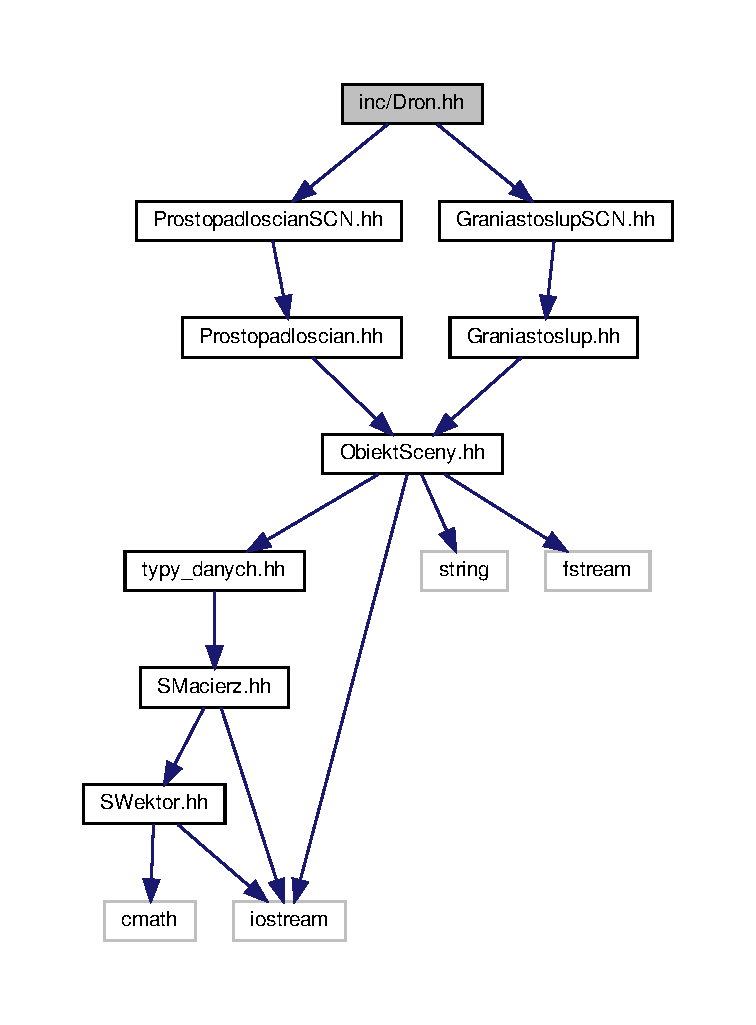
\includegraphics[width=350pt]{Dron_8hh__incl}
\end{center}
\end{figure}
Ten wykres pokazuje, które pliki bezpośrednio lub pośrednio załączają ten plik\+:\nopagebreak
\begin{figure}[H]
\begin{center}
\leavevmode
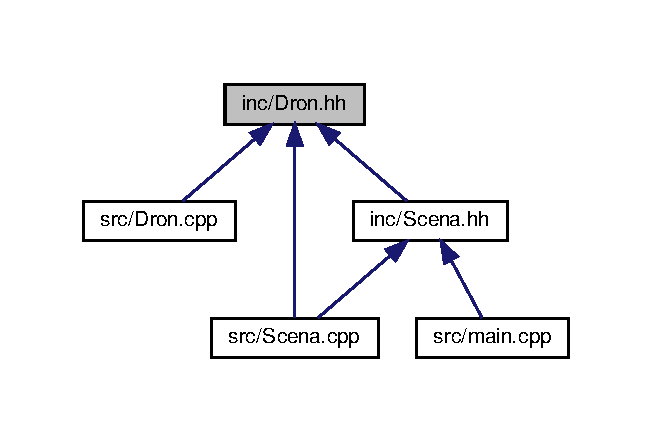
\includegraphics[width=313pt]{Dron_8hh__dep__incl}
\end{center}
\end{figure}
\subsection*{Komponenty}
\begin{DoxyCompactItemize}
\item 
class \hyperlink{classDron}{Dron}
\begin{DoxyCompactList}\small\item\em Definicja klasy \hyperlink{classDron}{Dron}. \end{DoxyCompactList}\end{DoxyCompactItemize}


\subsection{Opis szczegółowy}
Zawiera definicję klasy \hyperlink{classDron}{Dron}. 

Plik zawiera definicję klasy \hyperlink{classDron}{Dron}, sluzacej do interpretacji zadanego obiektu jako drona zdolnego do bycia przemieszczonym i obroconym z poziomu metod sceny. Elementami skladowymi drona sa obiekty klasy \hyperlink{classGraniastoslupSCN}{Graniastoslup\+S\+CN} oznaczajace sruby oraz jeden obiekt klasy \hyperlink{classProstopadloscianSCN}{Prostopadloscian\+S\+CN} oznaczajacy rdzen drona. \hyperlink{classDron}{Dron} ponadto jest w stanie wykryc kolizje z dostarczonym mu obiektem klasy \hyperlink{classObiektSceny}{Obiekt\+Sceny} 
\hypertarget{Graniastoslup_8hh}{}\section{Dokumentacja pliku inc/\+Graniastoslup.hh}
\label{Graniastoslup_8hh}\index{inc/\+Graniastoslup.\+hh@{inc/\+Graniastoslup.\+hh}}


Zawiera definicję klasy \hyperlink{classGraniastoslup}{Graniastoslup}.  


{\ttfamily \#include \char`\"{}Obiekt\+Sceny.\+hh\char`\"{}}\newline
Wykres zależności załączania dla Graniastoslup.\+hh\+:\nopagebreak
\begin{figure}[H]
\begin{center}
\leavevmode
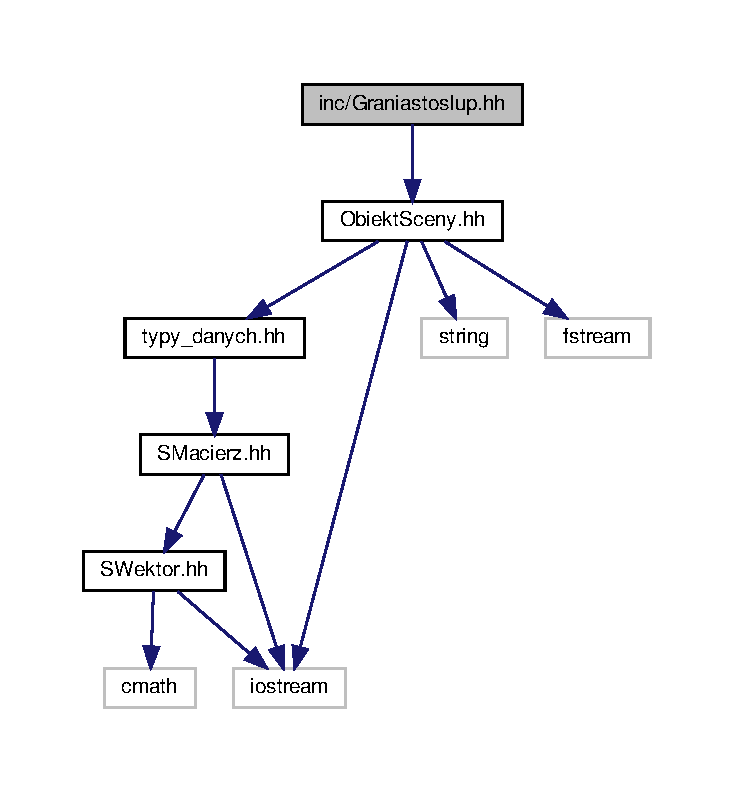
\includegraphics[width=350pt]{Graniastoslup_8hh__incl}
\end{center}
\end{figure}
Ten wykres pokazuje, które pliki bezpośrednio lub pośrednio załączają ten plik\+:\nopagebreak
\begin{figure}[H]
\begin{center}
\leavevmode
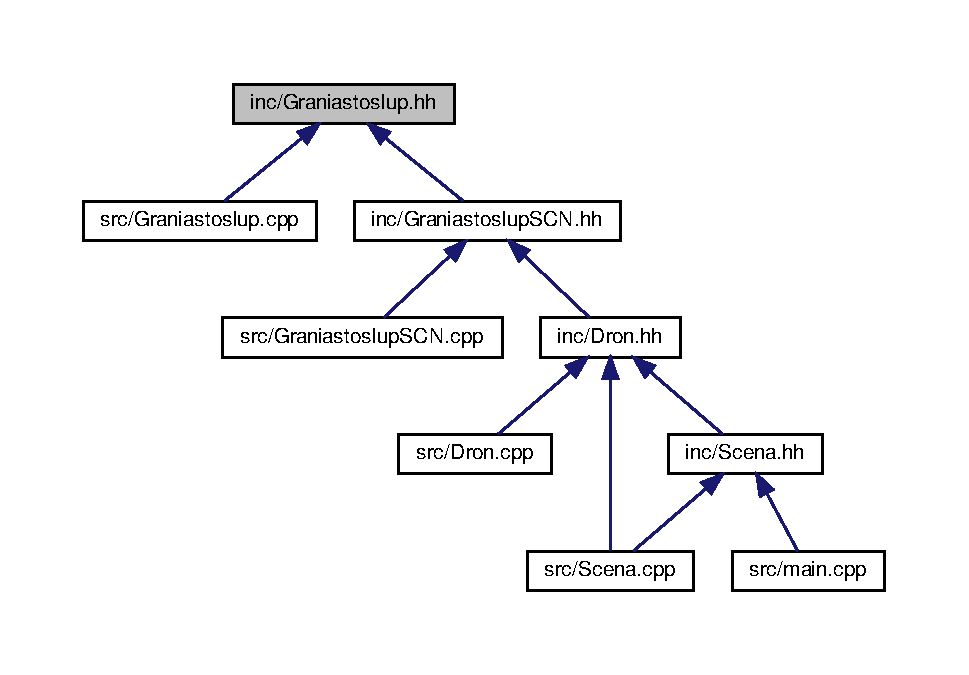
\includegraphics[width=350pt]{Graniastoslup_8hh__dep__incl}
\end{center}
\end{figure}
\subsection*{Komponenty}
\begin{DoxyCompactItemize}
\item 
class \hyperlink{classGraniastoslup}{Graniastoslup}
\begin{DoxyCompactList}\small\item\em \hyperlink{classGraniastoslup}{Graniastoslup} jako bryla przestrzenna o promieniu i srodku lokalnym. \end{DoxyCompactList}\end{DoxyCompactItemize}


\subsection{Opis szczegółowy}
Zawiera definicję klasy \hyperlink{classGraniastoslup}{Graniastoslup}. 

Plik zawiera definicję klasy \hyperlink{classGraniastoslup}{Graniastoslup}, sluzacej do interpretacji zadanego obiektu jako graniastoslupa majacego okreslone wspolrzedne w ukladzie kartezjanskim. Ponadto obiekt zapamietuje wartosc swojego promienia oraz lokalne polozenie swojego srodka. 
\hypertarget{GraniastoslupSCN_8hh}{}\section{Dokumentacja pliku inc/\+Graniastoslup\+S\+CN.hh}
\label{GraniastoslupSCN_8hh}\index{inc/\+Graniastoslup\+S\+C\+N.\+hh@{inc/\+Graniastoslup\+S\+C\+N.\+hh}}


Zawiera definicję klasy \hyperlink{classGraniastoslupSCN}{Graniastoslup\+S\+CN}.  


{\ttfamily \#include \char`\"{}Graniastoslup.\+hh\char`\"{}}\newline
Wykres zależności załączania dla Graniastoslup\+S\+C\+N.\+hh\+:\nopagebreak
\begin{figure}[H]
\begin{center}
\leavevmode
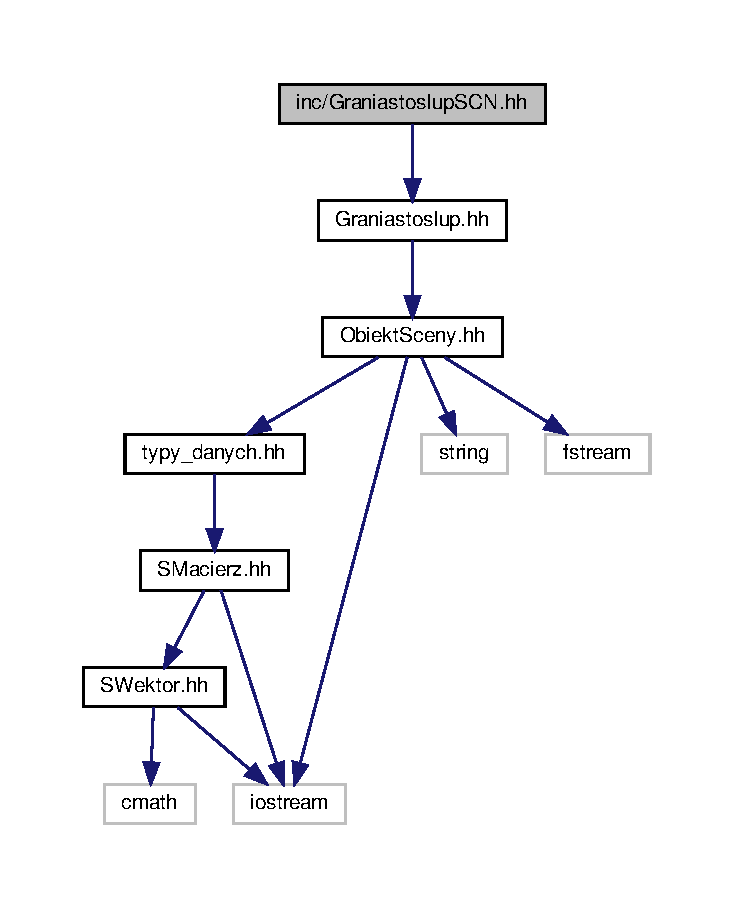
\includegraphics[width=350pt]{GraniastoslupSCN_8hh__incl}
\end{center}
\end{figure}
Ten wykres pokazuje, które pliki bezpośrednio lub pośrednio załączają ten plik\+:\nopagebreak
\begin{figure}[H]
\begin{center}
\leavevmode
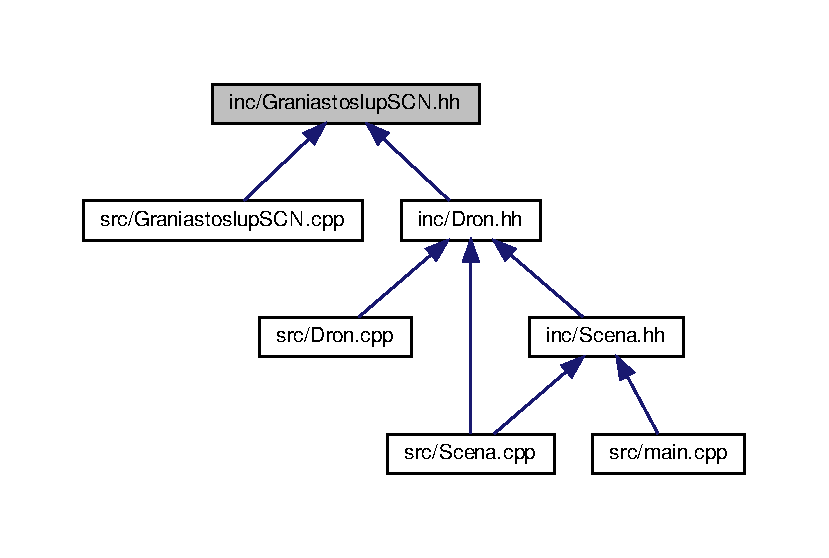
\includegraphics[width=350pt]{GraniastoslupSCN_8hh__dep__incl}
\end{center}
\end{figure}
\subsection*{Komponenty}
\begin{DoxyCompactItemize}
\item 
class \hyperlink{classGraniastoslupSCN}{Graniastoslup\+S\+CN}
\begin{DoxyCompactList}\small\item\em \hyperlink{classGraniastoslupSCN}{Graniastoslup\+S\+CN} jako \hyperlink{classGraniastoslup}{Graniastoslup} w ukladzie globalnym. \end{DoxyCompactList}\end{DoxyCompactItemize}


\subsection{Opis szczegółowy}
Zawiera definicję klasy \hyperlink{classGraniastoslupSCN}{Graniastoslup\+S\+CN}. 

Plik zawiera definicję klasy \hyperlink{classGraniastoslupSCN}{Graniastoslup\+S\+CN}, sluzacej do interpretacji zadanego graniastoslupa jako obiektu rozbudowanego o mozliwosc okreslenia orientacji i przesuniecia w ukladzie globalnym 
\hypertarget{lacze__do__gnuplota_8hh}{}\section{Dokumentacja pliku inc/lacze\+\_\+do\+\_\+gnuplota.hh}
\label{lacze__do__gnuplota_8hh}\index{inc/lacze\+\_\+do\+\_\+gnuplota.\+hh@{inc/lacze\+\_\+do\+\_\+gnuplota.\+hh}}


Zawiera definicję klasy \hyperlink{classPzG_1_1LaczeDoGNUPlota}{Pz\+G\+::\+Lacze\+Do\+G\+N\+U\+Plota}.  


{\ttfamily \#include $<$string$>$}\newline
{\ttfamily \#include $<$list$>$}\newline
{\ttfamily \#include $<$vector$>$}\newline
Wykres zależności załączania dla lacze\+\_\+do\+\_\+gnuplota.\+hh\+:\nopagebreak
\begin{figure}[H]
\begin{center}
\leavevmode
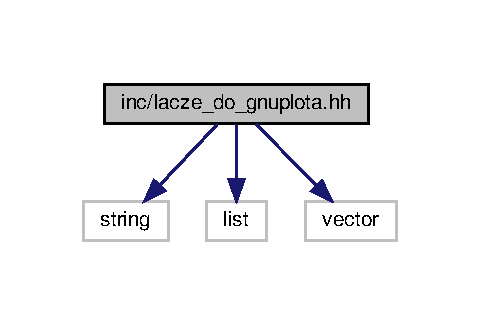
\includegraphics[width=231pt]{lacze__do__gnuplota_8hh__incl}
\end{center}
\end{figure}
Ten wykres pokazuje, które pliki bezpośrednio lub pośrednio załączają ten plik\+:\nopagebreak
\begin{figure}[H]
\begin{center}
\leavevmode
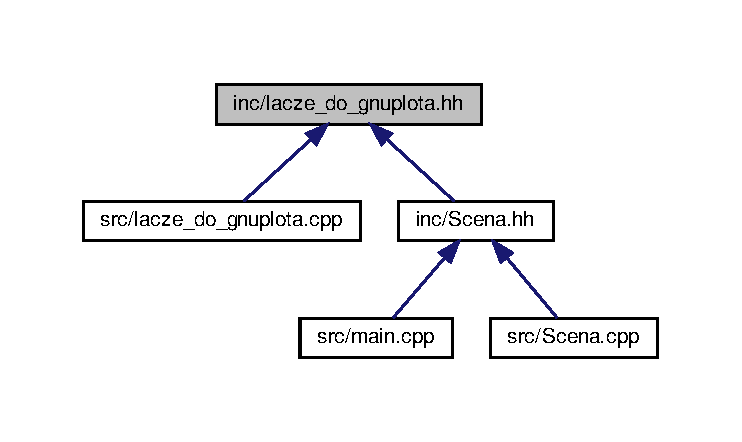
\includegraphics[width=350pt]{lacze__do__gnuplota_8hh__dep__incl}
\end{center}
\end{figure}
\subsection*{Komponenty}
\begin{DoxyCompactItemize}
\item 
class \hyperlink{classPzG_1_1InfoPlikuDoRysowania}{Pz\+G\+::\+Info\+Pliku\+Do\+Rysowania}
\begin{DoxyCompactList}\small\item\em Zestaw informacji dotyczący pliku i sposobu rysowania. \end{DoxyCompactList}\item 
class \hyperlink{classPzG_1_1LaczeDoGNUPlota}{Pz\+G\+::\+Lacze\+Do\+G\+N\+U\+Plota}
\begin{DoxyCompactList}\small\item\em Klasa realizuje interfejs do programu G\+N\+U\+Plot. \end{DoxyCompactList}\end{DoxyCompactItemize}
\subsection*{Przestrzenie nazw}
\begin{DoxyCompactItemize}
\item 
 \hyperlink{namespacePzG}{PzG}
\begin{DoxyCompactList}\small\item\em Moduł narzędzi umożliwiających połącznie z G\+N\+U\+Plotem. \end{DoxyCompactList}\end{DoxyCompactItemize}
\subsection*{Wyliczenia}
\begin{DoxyCompactItemize}
\item 
enum \hyperlink{namespacePzG_aeedae1ef10c66d720f9e89de408ca4ca}{Pz\+G\+::\+Tryb\+Rysowania} \{ {\bfseries T\+R\+\_\+2D}, 
{\bfseries T\+R\+\_\+3D}
 \}\begin{DoxyCompactList}\small\item\em Określa tryb rysowania realizowanego przez program {\ttfamily gnuplot}. \end{DoxyCompactList}
\item 
enum \hyperlink{namespacePzG_a705c92106f39b7d0c34a6739d10ff0b6}{Pz\+G\+::\+Rodzaj\+Rysowania} \{ {\bfseries R\+R\+\_\+\+Ciagly}, 
{\bfseries R\+R\+\_\+\+Punktowy}
 \}\begin{DoxyCompactList}\small\item\em Sposób rysowania linii. \end{DoxyCompactList}
\end{DoxyCompactItemize}


\subsection{Opis szczegółowy}
Zawiera definicję klasy \hyperlink{classPzG_1_1LaczeDoGNUPlota}{Pz\+G\+::\+Lacze\+Do\+G\+N\+U\+Plota}. 

Plik zawiera definicję klasy \hyperlink{classPzG_1_1LaczeDoGNUPlota}{Pz\+G\+::\+Lacze\+Do\+G\+N\+U\+Plota} realizującej interfejs komunikacyjny do programu gnuplot. 
\hypertarget{ObiektSceny_8hh}{}\section{Dokumentacja pliku inc/\+Obiekt\+Sceny.hh}
\label{ObiektSceny_8hh}\index{inc/\+Obiekt\+Sceny.\+hh@{inc/\+Obiekt\+Sceny.\+hh}}


Zawiera definicję klasy \hyperlink{classObiektSceny}{Obiekt\+Sceny}.  


{\ttfamily \#include \char`\"{}typy\+\_\+danych.\+hh\char`\"{}}\newline
{\ttfamily \#include $<$iostream$>$}\newline
{\ttfamily \#include $<$string$>$}\newline
{\ttfamily \#include $<$fstream$>$}\newline
Wykres zależności załączania dla Obiekt\+Sceny.\+hh\+:\nopagebreak
\begin{figure}[H]
\begin{center}
\leavevmode
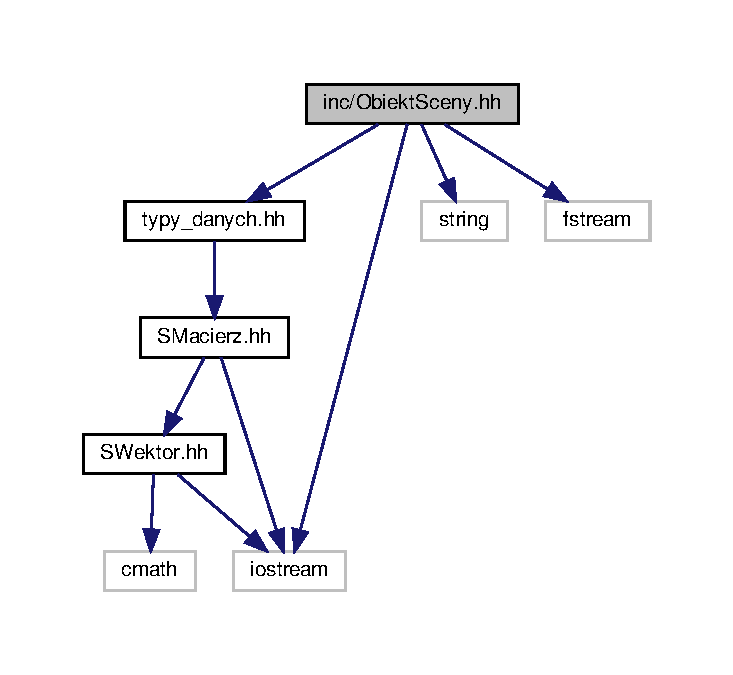
\includegraphics[width=350pt]{ObiektSceny_8hh__incl}
\end{center}
\end{figure}
Ten wykres pokazuje, które pliki bezpośrednio lub pośrednio załączają ten plik\+:\nopagebreak
\begin{figure}[H]
\begin{center}
\leavevmode
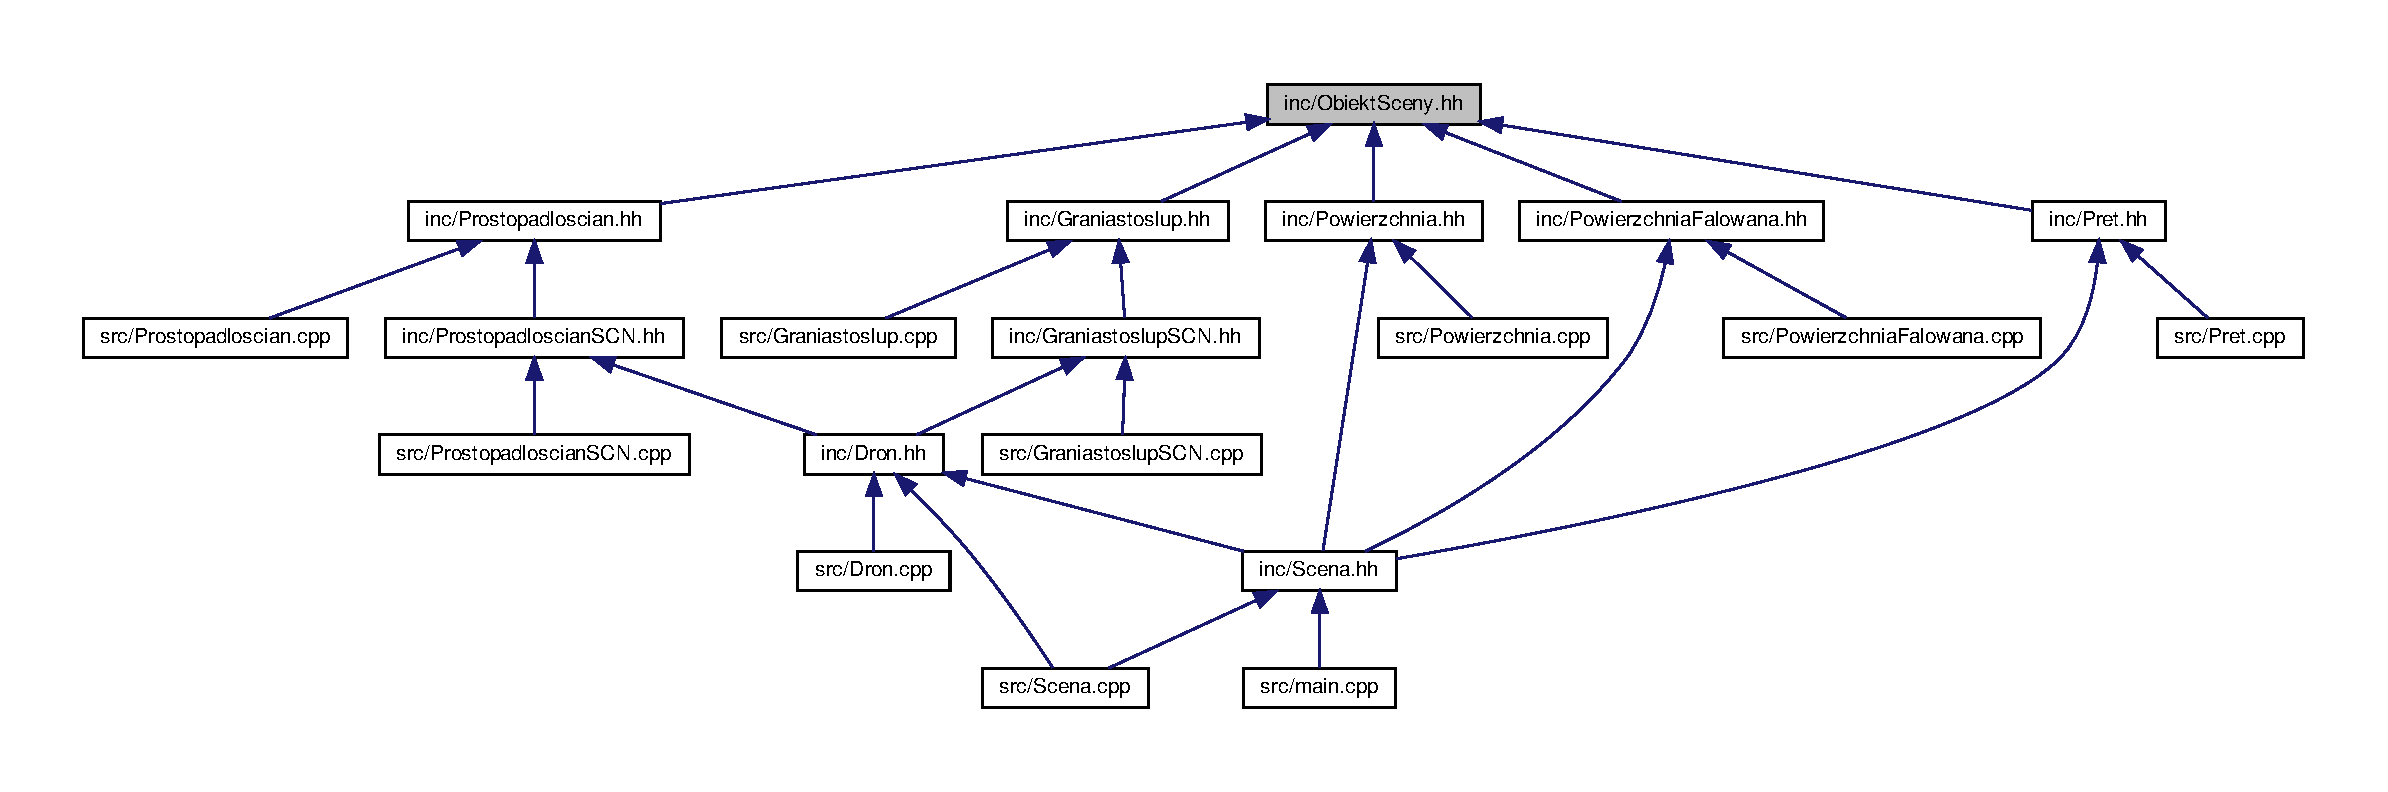
\includegraphics[width=350pt]{ObiektSceny_8hh__dep__incl}
\end{center}
\end{figure}
\subsection*{Komponenty}
\begin{DoxyCompactItemize}
\item 
class \hyperlink{classObiektSceny}{Obiekt\+Sceny}
\begin{DoxyCompactList}\small\item\em Definicja klasy \hyperlink{classObiektSceny}{Obiekt\+Sceny}. \end{DoxyCompactList}\end{DoxyCompactItemize}


\subsection{Opis szczegółowy}
Zawiera definicję klasy \hyperlink{classObiektSceny}{Obiekt\+Sceny}. 

Plik zawiera definicję klasy \hyperlink{classObiektSceny}{Obiekt\+Sceny}, sluzacej do ogólnenj interpretacji obiektów przestrzennych, mających okreslone wspolrzedne w ukladzie kartezjanskim. Ponadto obiekt zapamietuje wartosci swoich wspolrzednych skrajnych w celu umozliwienia bycia wykorzystanym do wykrycia kolizji. Klasa stanowi klase bazowa dla kazdej bryly reprezentowanej w pozostalej czesci programu. 
\hypertarget{Powierzchnia_8hh}{}\section{Dokumentacja pliku inc/\+Powierzchnia.hh}
\label{Powierzchnia_8hh}\index{inc/\+Powierzchnia.\+hh@{inc/\+Powierzchnia.\+hh}}


Zawiera definicję klasy \hyperlink{classPowierzchnia}{Powierzchnia}.  


{\ttfamily \#include \char`\"{}typy\+\_\+danych.\+hh\char`\"{}}\newline
{\ttfamily \#include \char`\"{}Obiekt\+Sceny.\+hh\char`\"{}}\newline
Wykres zależności załączania dla Powierzchnia.\+hh\+:\nopagebreak
\begin{figure}[H]
\begin{center}
\leavevmode
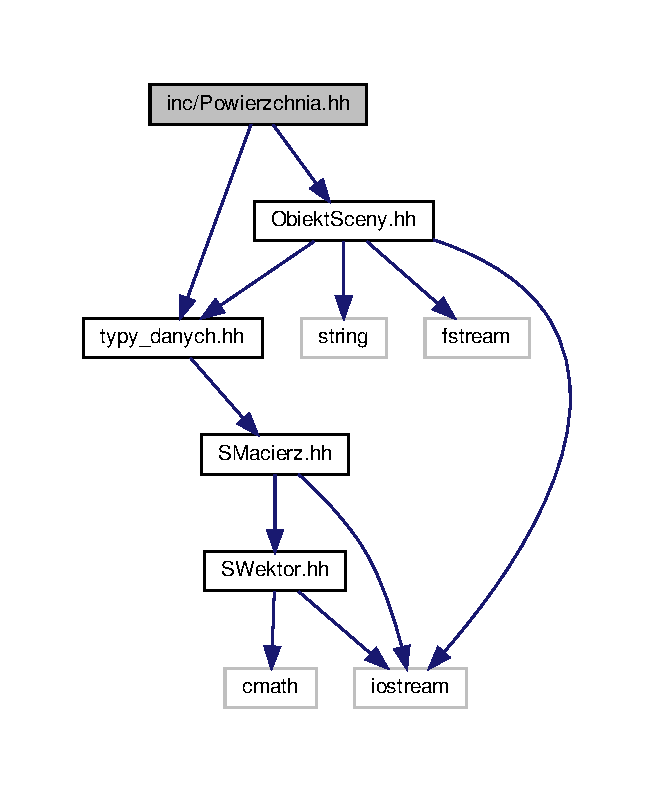
\includegraphics[width=314pt]{Powierzchnia_8hh__incl}
\end{center}
\end{figure}
Ten wykres pokazuje, które pliki bezpośrednio lub pośrednio załączają ten plik\+:\nopagebreak
\begin{figure}[H]
\begin{center}
\leavevmode
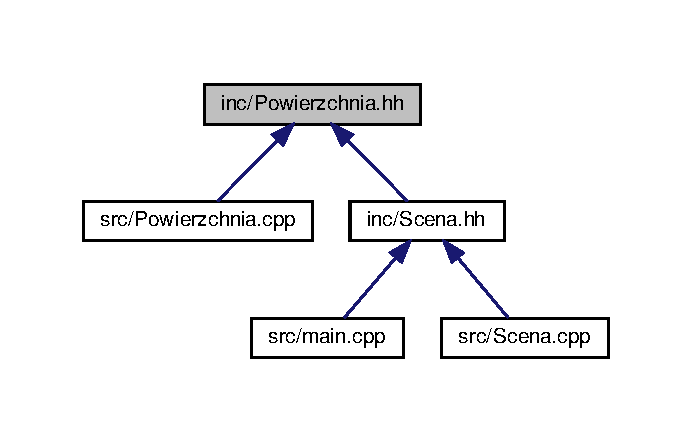
\includegraphics[width=332pt]{Powierzchnia_8hh__dep__incl}
\end{center}
\end{figure}
\subsection*{Komponenty}
\begin{DoxyCompactItemize}
\item 
class \hyperlink{classPowierzchnia}{Powierzchnia}
\begin{DoxyCompactList}\small\item\em \hyperlink{classPowierzchnia}{Powierzchnia} jako obiekt graficzny. \end{DoxyCompactList}\end{DoxyCompactItemize}


\subsection{Opis szczegółowy}
Zawiera definicję klasy \hyperlink{classPowierzchnia}{Powierzchnia}. 

Plik zawiera definicję klasy \hyperlink{classPowierzchnia}{Powierzchnia}, sluzacej do interpretacji zadanego obiektu jako powierzchni majacej okreslone wspolrzedne w ukladzie kartezjanskim. 
\hypertarget{PowierzchniaFalowana_8hh}{}\section{Dokumentacja pliku inc/\+Powierzchnia\+Falowana.hh}
\label{PowierzchniaFalowana_8hh}\index{inc/\+Powierzchnia\+Falowana.\+hh@{inc/\+Powierzchnia\+Falowana.\+hh}}


Zawiera definicję klasy \hyperlink{classPowierzchniaFalowana}{Powierzchnia\+Falowana}.  


{\ttfamily \#include \char`\"{}typy\+\_\+danych.\+hh\char`\"{}}\newline
{\ttfamily \#include \char`\"{}Obiekt\+Sceny.\+hh\char`\"{}}\newline
Wykres zależności załączania dla Powierzchnia\+Falowana.\+hh\+:\nopagebreak
\begin{figure}[H]
\begin{center}
\leavevmode
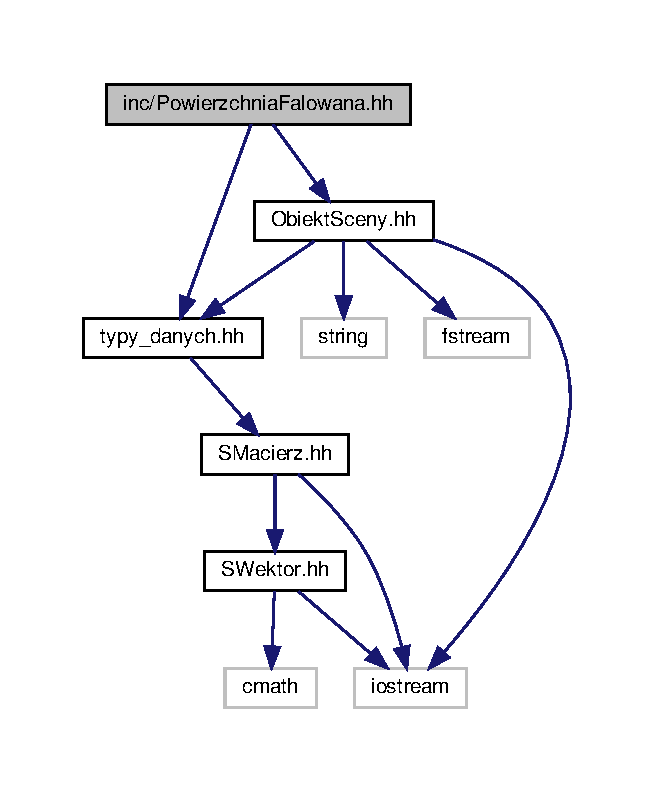
\includegraphics[width=314pt]{PowierzchniaFalowana_8hh__incl}
\end{center}
\end{figure}
Ten wykres pokazuje, które pliki bezpośrednio lub pośrednio załączają ten plik\+:\nopagebreak
\begin{figure}[H]
\begin{center}
\leavevmode
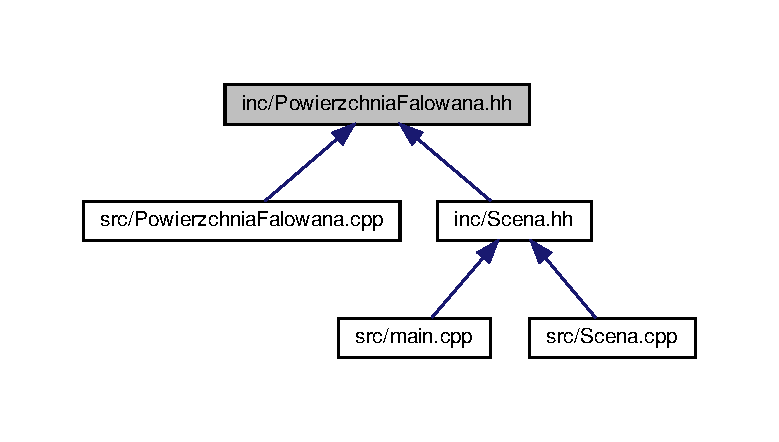
\includegraphics[width=350pt]{PowierzchniaFalowana_8hh__dep__incl}
\end{center}
\end{figure}
\subsection*{Komponenty}
\begin{DoxyCompactItemize}
\item 
class \hyperlink{classPowierzchniaFalowana}{Powierzchnia\+Falowana}
\begin{DoxyCompactList}\small\item\em \hyperlink{classPowierzchniaFalowana}{Powierzchnia\+Falowana} jako obiekt graficzny. \end{DoxyCompactList}\end{DoxyCompactItemize}


\subsection{Opis szczegółowy}
Zawiera definicję klasy \hyperlink{classPowierzchniaFalowana}{Powierzchnia\+Falowana}. 

Plik zawiera definicję klasy \hyperlink{classPowierzchniaFalowana}{Powierzchnia\+Falowana}, sluzacej do interpretacji zadanego obiektu jako powierzchni falowanej majacej okreslone wspolrzedne w ukladzie kartezjanskim. 
\hypertarget{Pret_8hh}{}\section{Dokumentacja pliku inc/\+Pret.hh}
\label{Pret_8hh}\index{inc/\+Pret.\+hh@{inc/\+Pret.\+hh}}


Zawiera definicję klasy \hyperlink{classPret}{Pret}.  


{\ttfamily \#include \char`\"{}typy\+\_\+danych.\+hh\char`\"{}}\newline
{\ttfamily \#include \char`\"{}Obiekt\+Sceny.\+hh\char`\"{}}\newline
Wykres zależności załączania dla Pret.\+hh\+:\nopagebreak
\begin{figure}[H]
\begin{center}
\leavevmode
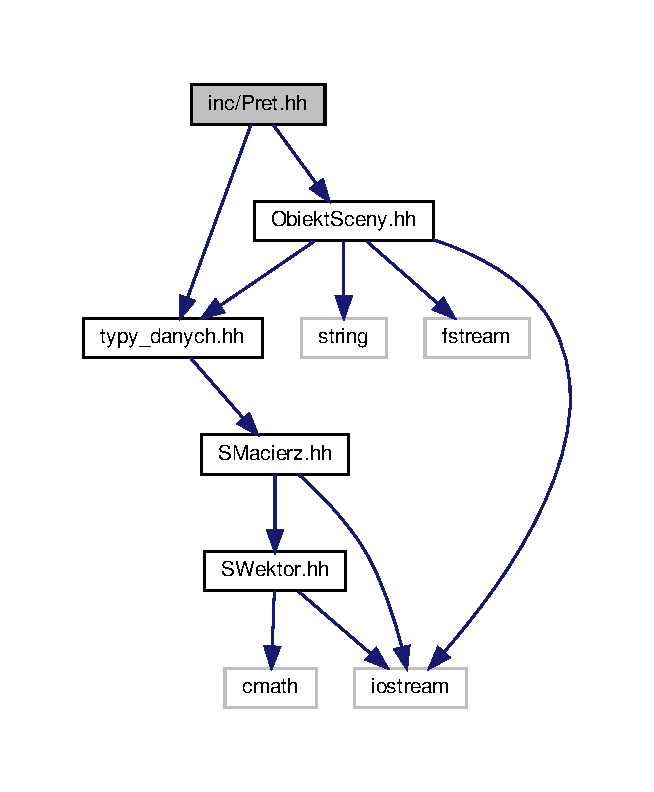
\includegraphics[width=314pt]{Pret_8hh__incl}
\end{center}
\end{figure}
Ten wykres pokazuje, które pliki bezpośrednio lub pośrednio załączają ten plik\+:\nopagebreak
\begin{figure}[H]
\begin{center}
\leavevmode
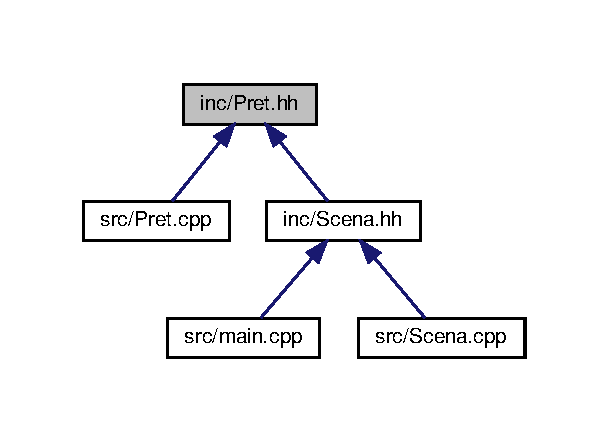
\includegraphics[width=292pt]{Pret_8hh__dep__incl}
\end{center}
\end{figure}
\subsection*{Komponenty}
\begin{DoxyCompactItemize}
\item 
class \hyperlink{classPret}{Pret}
\begin{DoxyCompactList}\small\item\em \hyperlink{classPret}{Pret} jako obiekt graficzny. \end{DoxyCompactList}\end{DoxyCompactItemize}


\subsection{Opis szczegółowy}
Zawiera definicję klasy \hyperlink{classPret}{Pret}. 

Plik zawiera definicję klasy \hyperlink{classPret}{Pret}, sluzacej do interpretacji zadanego obiektu jako preta majacego okreslone wspolrzedne w ukladzie kartezjanskim. 
\hypertarget{Prostopadloscian_8hh}{}\section{Dokumentacja pliku inc/\+Prostopadloscian.hh}
\label{Prostopadloscian_8hh}\index{inc/\+Prostopadloscian.\+hh@{inc/\+Prostopadloscian.\+hh}}


Zawiera definicję klasy \hyperlink{classProstopadloscian}{Prostopadloscian}.  


{\ttfamily \#include \char`\"{}Obiekt\+Sceny.\+hh\char`\"{}}\newline
Wykres zależności załączania dla Prostopadloscian.\+hh\+:\nopagebreak
\begin{figure}[H]
\begin{center}
\leavevmode
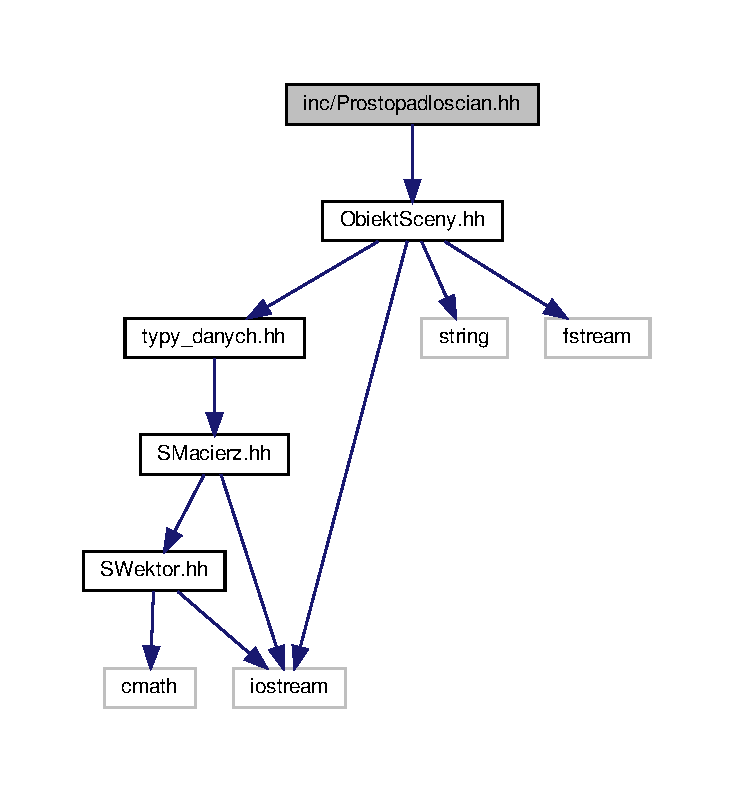
\includegraphics[width=350pt]{Prostopadloscian_8hh__incl}
\end{center}
\end{figure}
Ten wykres pokazuje, które pliki bezpośrednio lub pośrednio załączają ten plik\+:\nopagebreak
\begin{figure}[H]
\begin{center}
\leavevmode
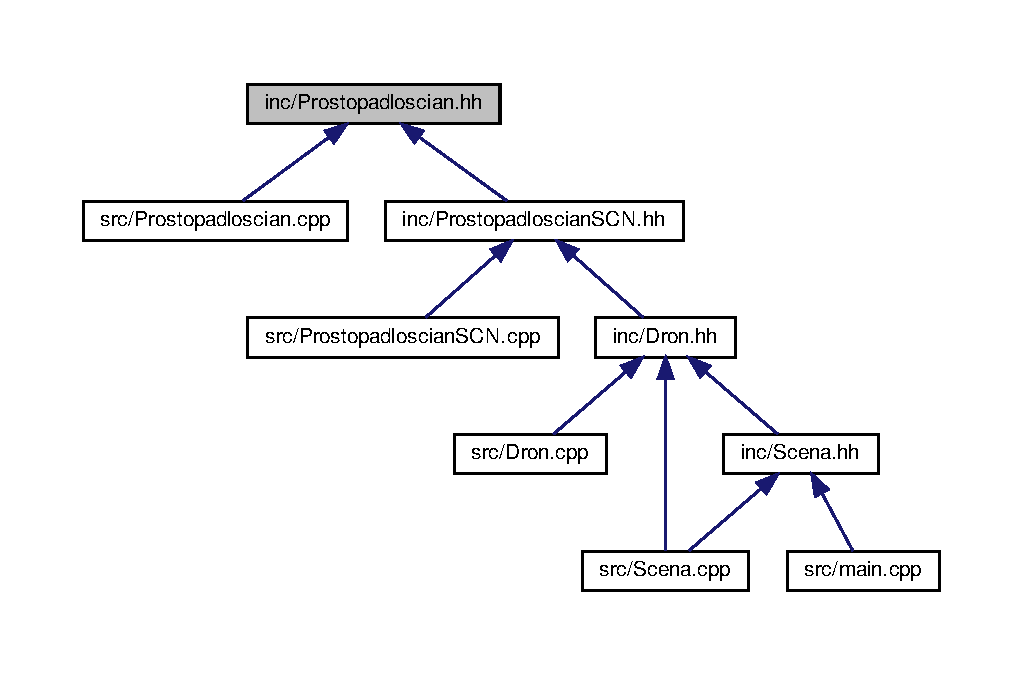
\includegraphics[width=350pt]{Prostopadloscian_8hh__dep__incl}
\end{center}
\end{figure}
\subsection*{Komponenty}
\begin{DoxyCompactItemize}
\item 
class \hyperlink{classProstopadloscian}{Prostopadloscian}
\begin{DoxyCompactList}\small\item\em \hyperlink{classProstopadloscian}{Prostopadloscian} jako bryla przestrzenna o promieniu i srodku lokalnym. \end{DoxyCompactList}\end{DoxyCompactItemize}


\subsection{Opis szczegółowy}
Zawiera definicję klasy \hyperlink{classProstopadloscian}{Prostopadloscian}. 

Plik zawiera definicję klasy \hyperlink{classProstopadloscian}{Prostopadloscian}, sluzacej do interpretacji zadanego obiektu jako prostopadloscianu majacego okreslone wspolrzedne w ukladzie kartezjanskim. Ponadto obiekt zapamietuje wartosc swojego promienia oraz lokalne polozenie swojego srodka. 
\hypertarget{ProstopadloscianSCN_8hh}{}\section{Dokumentacja pliku inc/\+Prostopadloscian\+S\+CN.hh}
\label{ProstopadloscianSCN_8hh}\index{inc/\+Prostopadloscian\+S\+C\+N.\+hh@{inc/\+Prostopadloscian\+S\+C\+N.\+hh}}


Zawiera definicję klasy \hyperlink{classProstopadloscianSCN}{Prostopadloscian\+S\+CN}.  


{\ttfamily \#include \char`\"{}Prostopadloscian.\+hh\char`\"{}}\newline
Wykres zależności załączania dla Prostopadloscian\+S\+C\+N.\+hh\+:\nopagebreak
\begin{figure}[H]
\begin{center}
\leavevmode
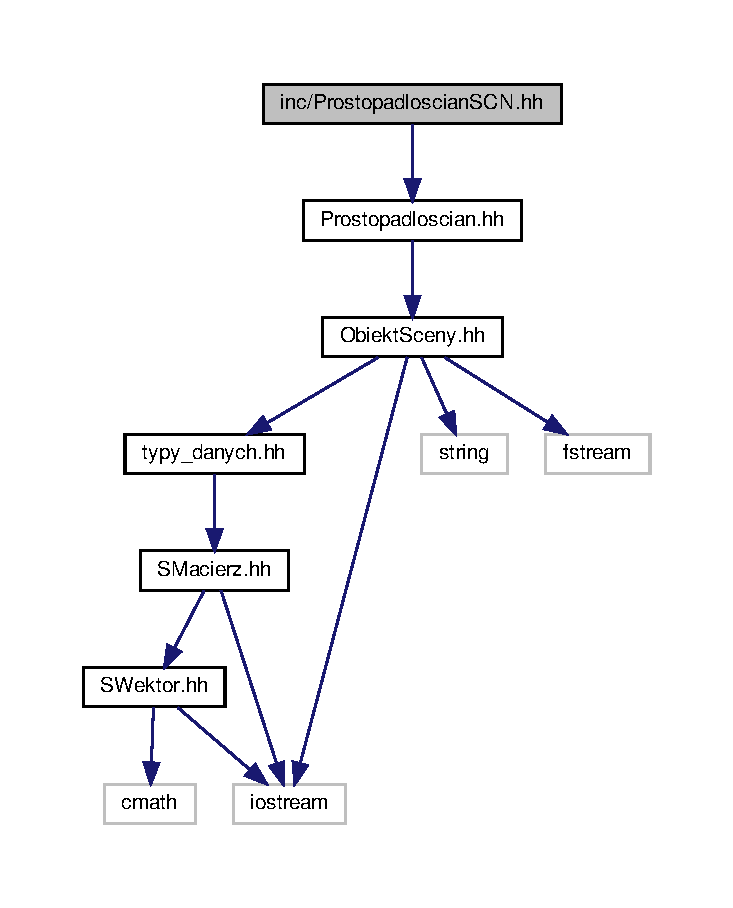
\includegraphics[width=350pt]{ProstopadloscianSCN_8hh__incl}
\end{center}
\end{figure}
Ten wykres pokazuje, które pliki bezpośrednio lub pośrednio załączają ten plik\+:\nopagebreak
\begin{figure}[H]
\begin{center}
\leavevmode
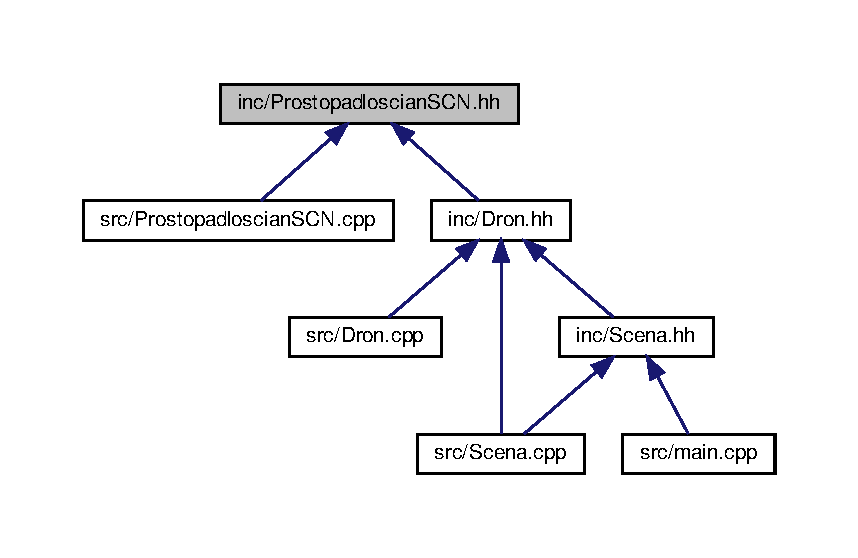
\includegraphics[width=350pt]{ProstopadloscianSCN_8hh__dep__incl}
\end{center}
\end{figure}
\subsection*{Komponenty}
\begin{DoxyCompactItemize}
\item 
class \hyperlink{classProstopadloscianSCN}{Prostopadloscian\+S\+CN}
\begin{DoxyCompactList}\small\item\em \hyperlink{classProstopadloscianSCN}{Prostopadloscian\+S\+CN} jako \hyperlink{classProstopadloscian}{Prostopadloscian} w ukladzie globalnym. \end{DoxyCompactList}\end{DoxyCompactItemize}


\subsection{Opis szczegółowy}
Zawiera definicję klasy \hyperlink{classProstopadloscianSCN}{Prostopadloscian\+S\+CN}. 

Plik zawiera definicję klasy \hyperlink{classProstopadloscianSCN}{Prostopadloscian\+S\+CN}, sluzacej do interpretacji zadanego prostopadloscianu jako obiektu rozbudowanego o mozliwosc okreslenia orientacji i przesuniecia w ukladzie globalnym 
\hypertarget{Scena_8hh}{}\section{Dokumentacja pliku inc/\+Scena.hh}
\label{Scena_8hh}\index{inc/\+Scena.\+hh@{inc/\+Scena.\+hh}}


Zawiera definicję klasy \hyperlink{classScena}{Scena}.  


{\ttfamily \#include \char`\"{}Dron.\+hh\char`\"{}}\newline
{\ttfamily \#include \char`\"{}lacze\+\_\+do\+\_\+gnuplota.\+hh\char`\"{}}\newline
{\ttfamily \#include \char`\"{}Powierzchnia.\+hh\char`\"{}}\newline
{\ttfamily \#include \char`\"{}Powierzchnia\+Falowana.\+hh\char`\"{}}\newline
{\ttfamily \#include \char`\"{}Pret.\+hh\char`\"{}}\newline
{\ttfamily \#include $<$unistd.\+h$>$}\newline
Wykres zależności załączania dla Scena.\+hh\+:\nopagebreak
\begin{figure}[H]
\begin{center}
\leavevmode
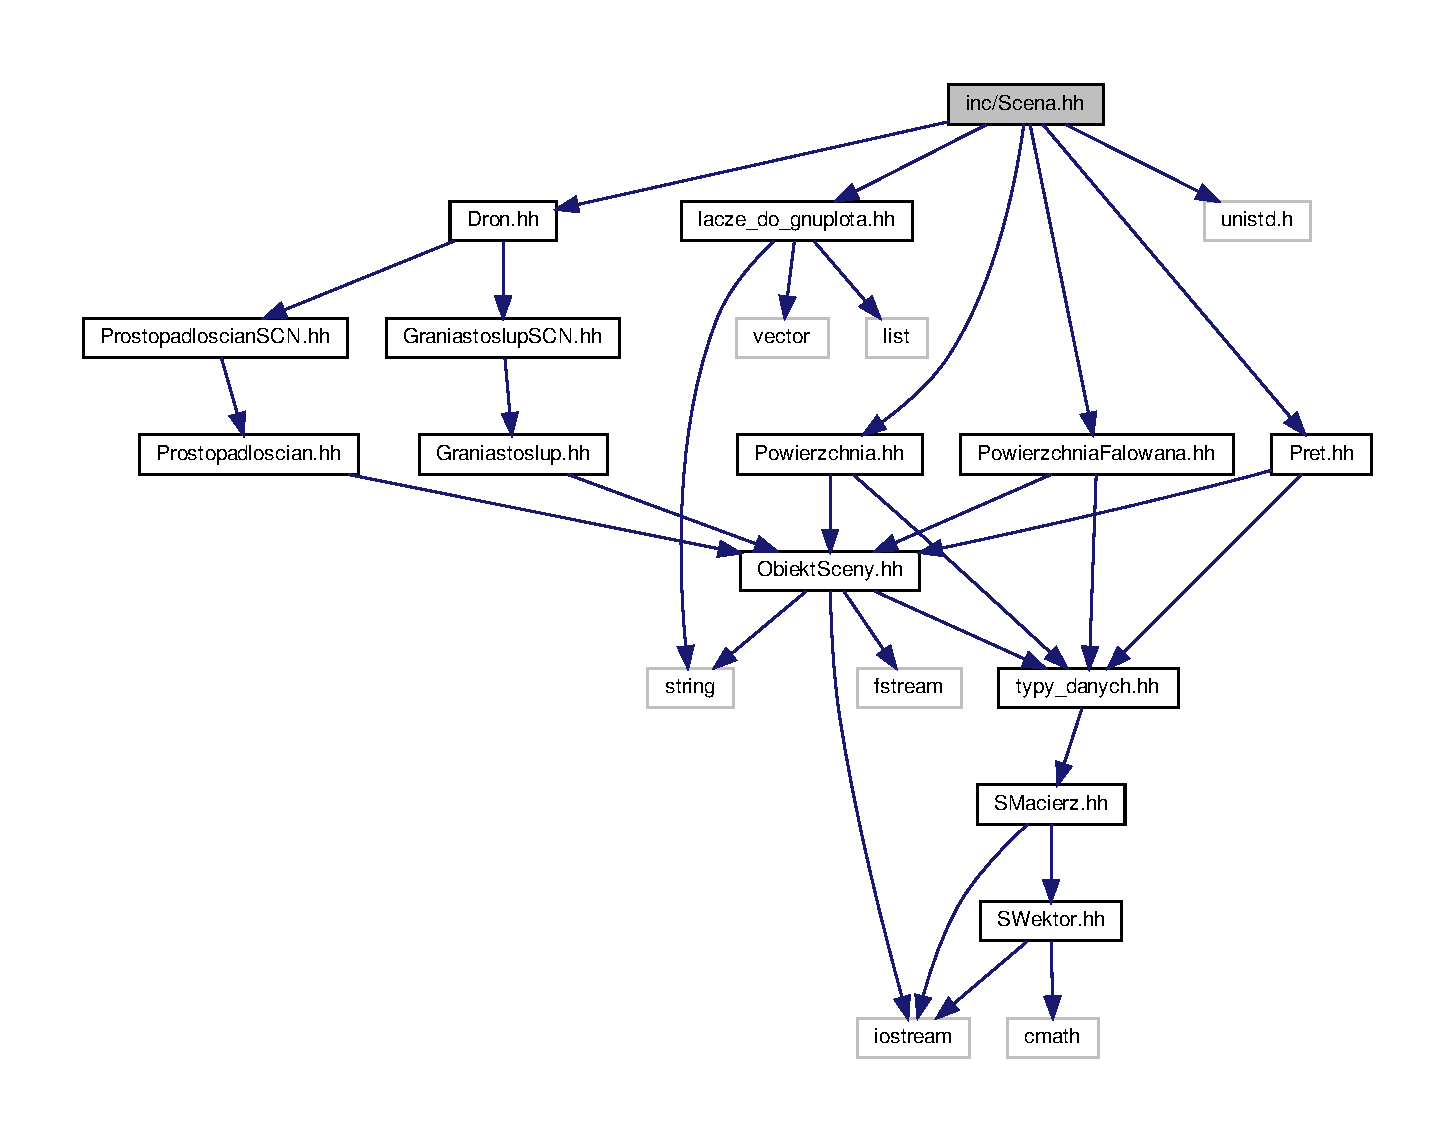
\includegraphics[width=350pt]{Scena_8hh__incl}
\end{center}
\end{figure}
Ten wykres pokazuje, które pliki bezpośrednio lub pośrednio załączają ten plik\+:\nopagebreak
\begin{figure}[H]
\begin{center}
\leavevmode
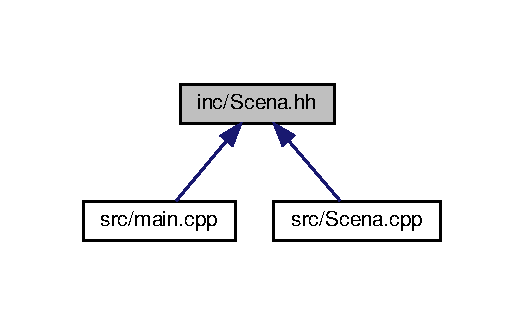
\includegraphics[width=252pt]{Scena_8hh__dep__incl}
\end{center}
\end{figure}
\subsection*{Komponenty}
\begin{DoxyCompactItemize}
\item 
class \hyperlink{classScena}{Scena}
\begin{DoxyCompactList}\small\item\em \hyperlink{classScena}{Scena} jako klasa zarzadzajaca obiektami graficznymi. \end{DoxyCompactList}\end{DoxyCompactItemize}


\subsection{Opis szczegółowy}
Zawiera definicję klasy \hyperlink{classScena}{Scena}. 

Plik zawiera definicję klasy \hyperlink{classScena}{Scena}, sluzacej do zarzadzania graficznymi interpretacjami obiektow wykorzystywanych przez program. 
\hypertarget{SMacierz_8hh}{}\section{Dokumentacja pliku inc/\+S\+Macierz.hh}
\label{SMacierz_8hh}\index{inc/\+S\+Macierz.\+hh@{inc/\+S\+Macierz.\+hh}}


Plik zawiera definicje szablonu macierzy kwadratowej.  


{\ttfamily \#include $<$iostream$>$}\newline
{\ttfamily \#include \char`\"{}S\+Wektor.\+hh\char`\"{}}\newline
Wykres zależności załączania dla S\+Macierz.\+hh\+:\nopagebreak
\begin{figure}[H]
\begin{center}
\leavevmode
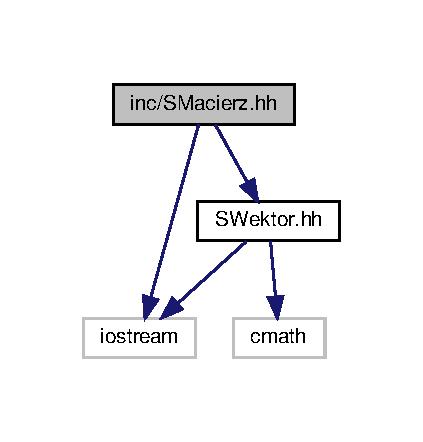
\includegraphics[width=203pt]{SMacierz_8hh__incl}
\end{center}
\end{figure}
Ten wykres pokazuje, które pliki bezpośrednio lub pośrednio załączają ten plik\+:\nopagebreak
\begin{figure}[H]
\begin{center}
\leavevmode
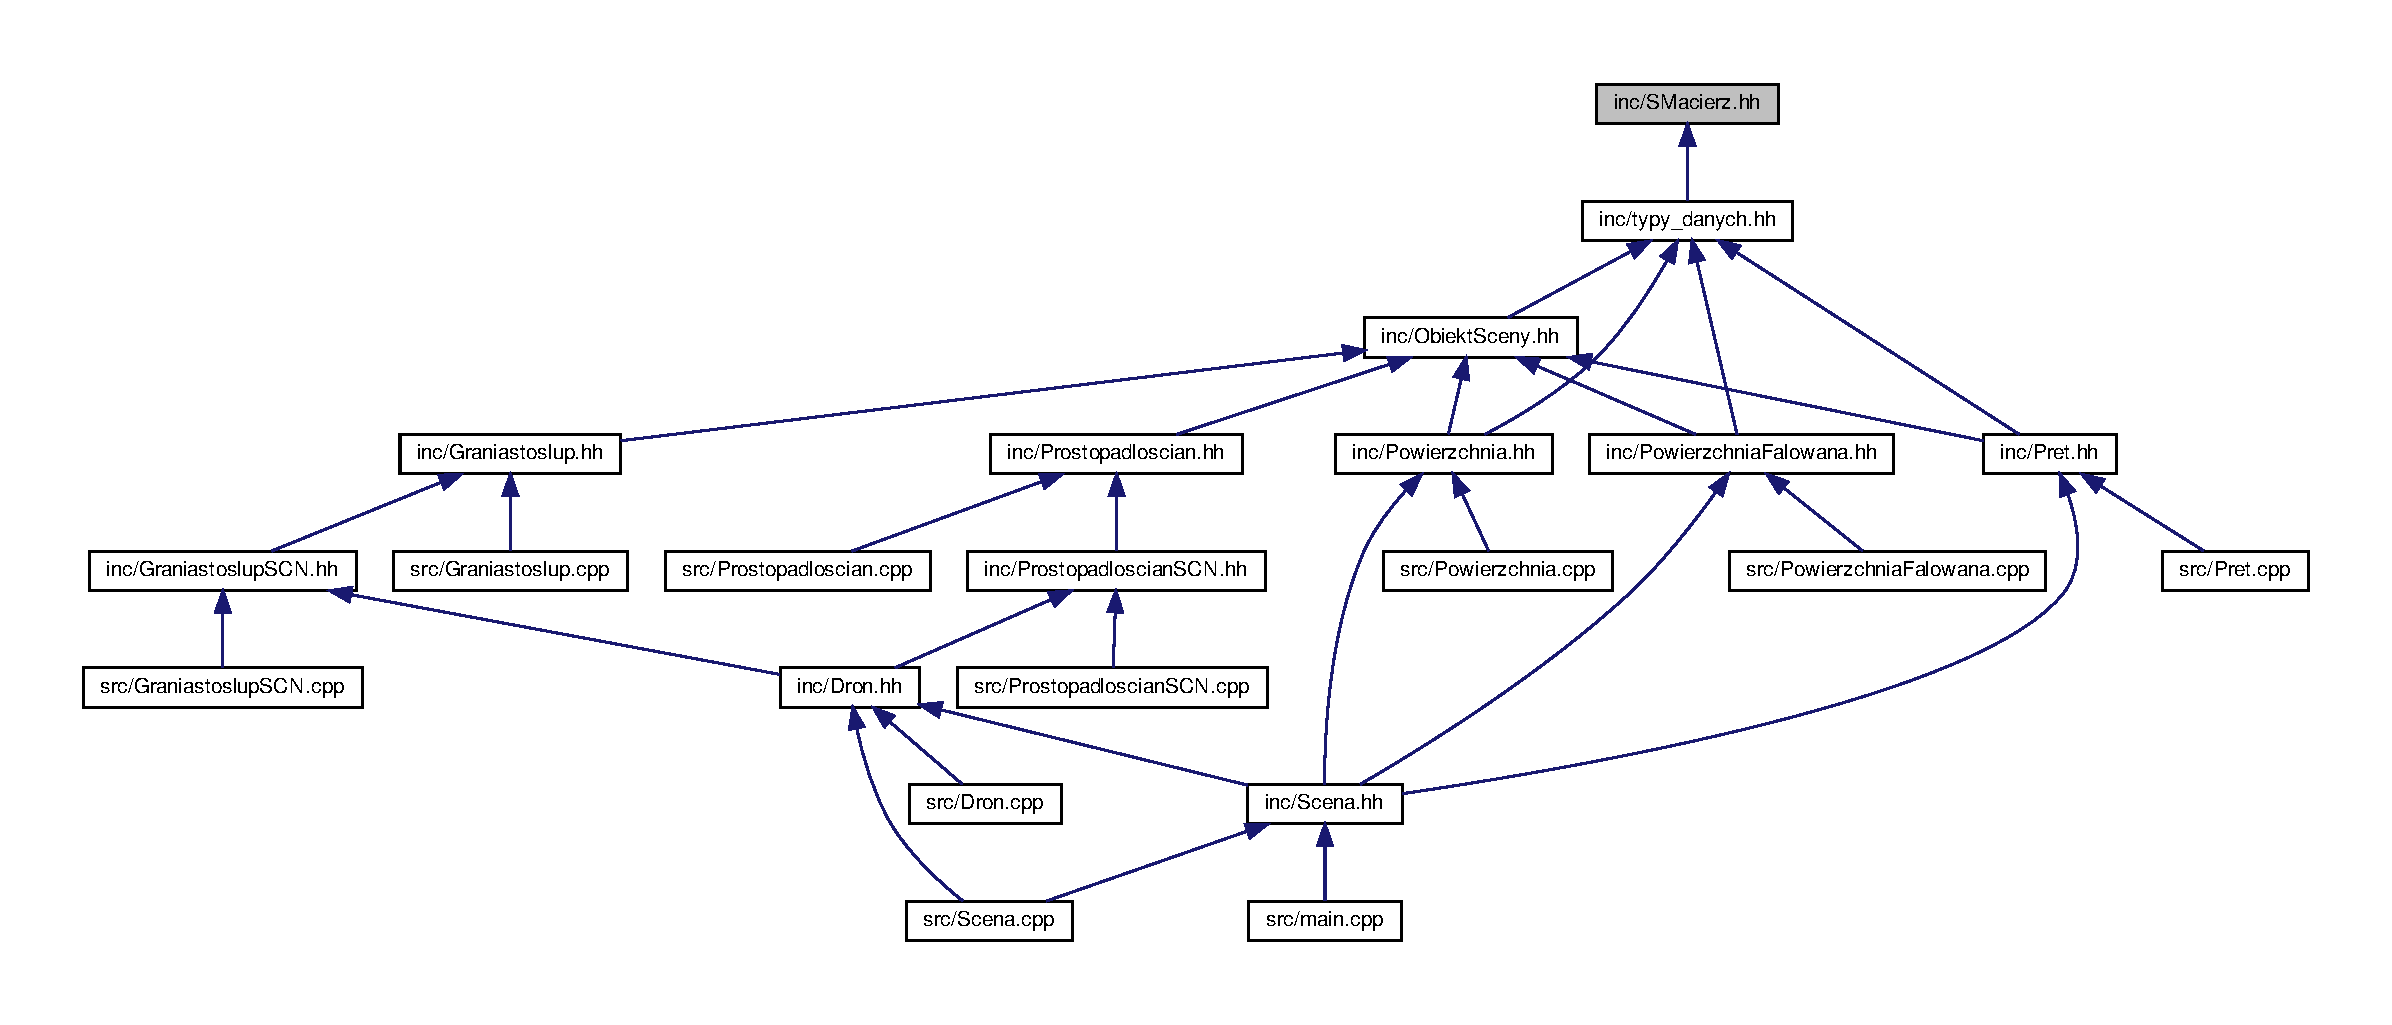
\includegraphics[width=350pt]{SMacierz_8hh__dep__incl}
\end{center}
\end{figure}
\subsection*{Komponenty}
\begin{DoxyCompactItemize}
\item 
class \hyperlink{classSMacierz}{S\+Macierz$<$ Typ, Wymiar $>$}
\begin{DoxyCompactList}\small\item\em Klasa modeluje pojęcie macierzy kwadratowej. \end{DoxyCompactList}\end{DoxyCompactItemize}
\subsection*{Funkcje}
\begin{DoxyCompactItemize}
\item 
{\footnotesize template$<$typename Typ , int Wymiar$>$ }\\std\+::ostream \& \hyperlink{SMacierz_8hh_aac60a3b8819068881df97089a29e7846}{operator$<$$<$} (std\+::ostream \&Strm\+Wy, const \hyperlink{classSMacierz}{S\+Macierz}$<$ Typ, Wymiar $>$ \&Mac)
\begin{DoxyCompactList}\small\item\em Realizuje wyswietlenie elementow macierzy na strumien wyjsciowy. \end{DoxyCompactList}\item 
{\footnotesize template$<$typename Typ , int Wymiar$>$ }\\std\+::istream \& \hyperlink{SMacierz_8hh_a15cb0e176b1de7cb59fa98f93c3c55e5}{operator$>$$>$} (std\+::istream \&Strm\+We, \hyperlink{classSMacierz}{S\+Macierz}$<$ Typ, Wymiar $>$ \&Mac)
\end{DoxyCompactItemize}


\subsection{Opis szczegółowy}
Plik zawiera definicje szablonu macierzy kwadratowej. 

Plik zawiera szablon klasy modelujacej pojęcie macierzy jako jednowymiarowej tablicy wektorów o wielkości \char`\"{}\+Wymiar\char`\"{}. Zawiera ona metody umożliwiające pobranie wartosci wybranego pola z wybranego wektora tablicy klasy, czy też jego modyfikację. Ponadto umożliwia wykonanie mnożenia macierzy przez wektor, wyliczenie wyznacznika, transpozycję macierzy oraz podstawienie jednej macierzy do drugiej. 

\subsection{Dokumentacja funkcji}
\mbox{\Hypertarget{SMacierz_8hh_aac60a3b8819068881df97089a29e7846}\label{SMacierz_8hh_aac60a3b8819068881df97089a29e7846}} 
\index{S\+Macierz.\+hh@{S\+Macierz.\+hh}!operator$<$$<$@{operator$<$$<$}}
\index{operator$<$$<$@{operator$<$$<$}!S\+Macierz.\+hh@{S\+Macierz.\+hh}}
\subsubsection{\texorpdfstring{operator$<$$<$()}{operator<<()}}
{\footnotesize\ttfamily template$<$typename Typ , int Wymiar$>$ \\
std\+::ostream\& operator$<$$<$ (\begin{DoxyParamCaption}\item[{std\+::ostream \&}]{Strm\+Wy,  }\item[{const \hyperlink{classSMacierz}{S\+Macierz}$<$ Typ, Wymiar $>$ \&}]{Mac }\end{DoxyParamCaption})}



Realizuje wyswietlenie elementow macierzy na strumien wyjsciowy. 

Realizuje wyswietlenie elementow macierzy na strumien wyjsciowy. 
\begin{DoxyParams}[1]{Parametry}
\mbox{\tt in}  & {\em Srm\+Wy} & -\/ referencja do strumienia wyjsciowego -\/ obiektu ostream \\
\hline
\mbox{\tt in}  & {\em Mac} & -\/ referencja do stałej, wyswietlanej macierzy -\/ obiektu klasy \hyperlink{classSMacierz}{S\+Macierz} \\
\hline
\end{DoxyParams}

\begin{DoxyRetVals}{Zwracane wartości}
{\em Referencja} & do strumienia wyjsciowego \\
\hline
\end{DoxyRetVals}
\mbox{\Hypertarget{SMacierz_8hh_a15cb0e176b1de7cb59fa98f93c3c55e5}\label{SMacierz_8hh_a15cb0e176b1de7cb59fa98f93c3c55e5}} 
\index{S\+Macierz.\+hh@{S\+Macierz.\+hh}!operator$>$$>$@{operator$>$$>$}}
\index{operator$>$$>$@{operator$>$$>$}!S\+Macierz.\+hh@{S\+Macierz.\+hh}}
\subsubsection{\texorpdfstring{operator$>$$>$()}{operator>>()}}
{\footnotesize\ttfamily template$<$typename Typ , int Wymiar$>$ \\
std\+::istream\& operator$>$$>$ (\begin{DoxyParamCaption}\item[{std\+::istream \&}]{Strm\+We,  }\item[{\hyperlink{classSMacierz}{S\+Macierz}$<$ Typ, Wymiar $>$ \&}]{Mac }\end{DoxyParamCaption})}

Wczytuje elementy macierzy na podstawie danych ze strumienia wejsciowego. Argumenty\+: Srm\+We -\/ referencja do strumienia wejsciowego -\/ obiektu istream Mac -\/ referencja do wczytywanej macierzy -\/ obiektu klasy \hyperlink{classSMacierz}{S\+Macierz} Zwraca\+: Referencje do strumienia wejsciowego 
\hypertarget{SWektor_8hh}{}\section{Dokumentacja pliku inc/\+S\+Wektor.hh}
\label{SWektor_8hh}\index{inc/\+S\+Wektor.\+hh@{inc/\+S\+Wektor.\+hh}}


Plik zawiera szablon klasy modelujacej pojecie wektora.  


{\ttfamily \#include $<$iostream$>$}\newline
{\ttfamily \#include $<$cmath$>$}\newline
Wykres zależności załączania dla S\+Wektor.\+hh\+:\nopagebreak
\begin{figure}[H]
\begin{center}
\leavevmode
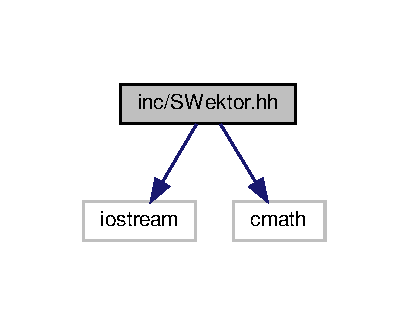
\includegraphics[width=196pt]{SWektor_8hh__incl}
\end{center}
\end{figure}
Ten wykres pokazuje, które pliki bezpośrednio lub pośrednio załączają ten plik\+:\nopagebreak
\begin{figure}[H]
\begin{center}
\leavevmode
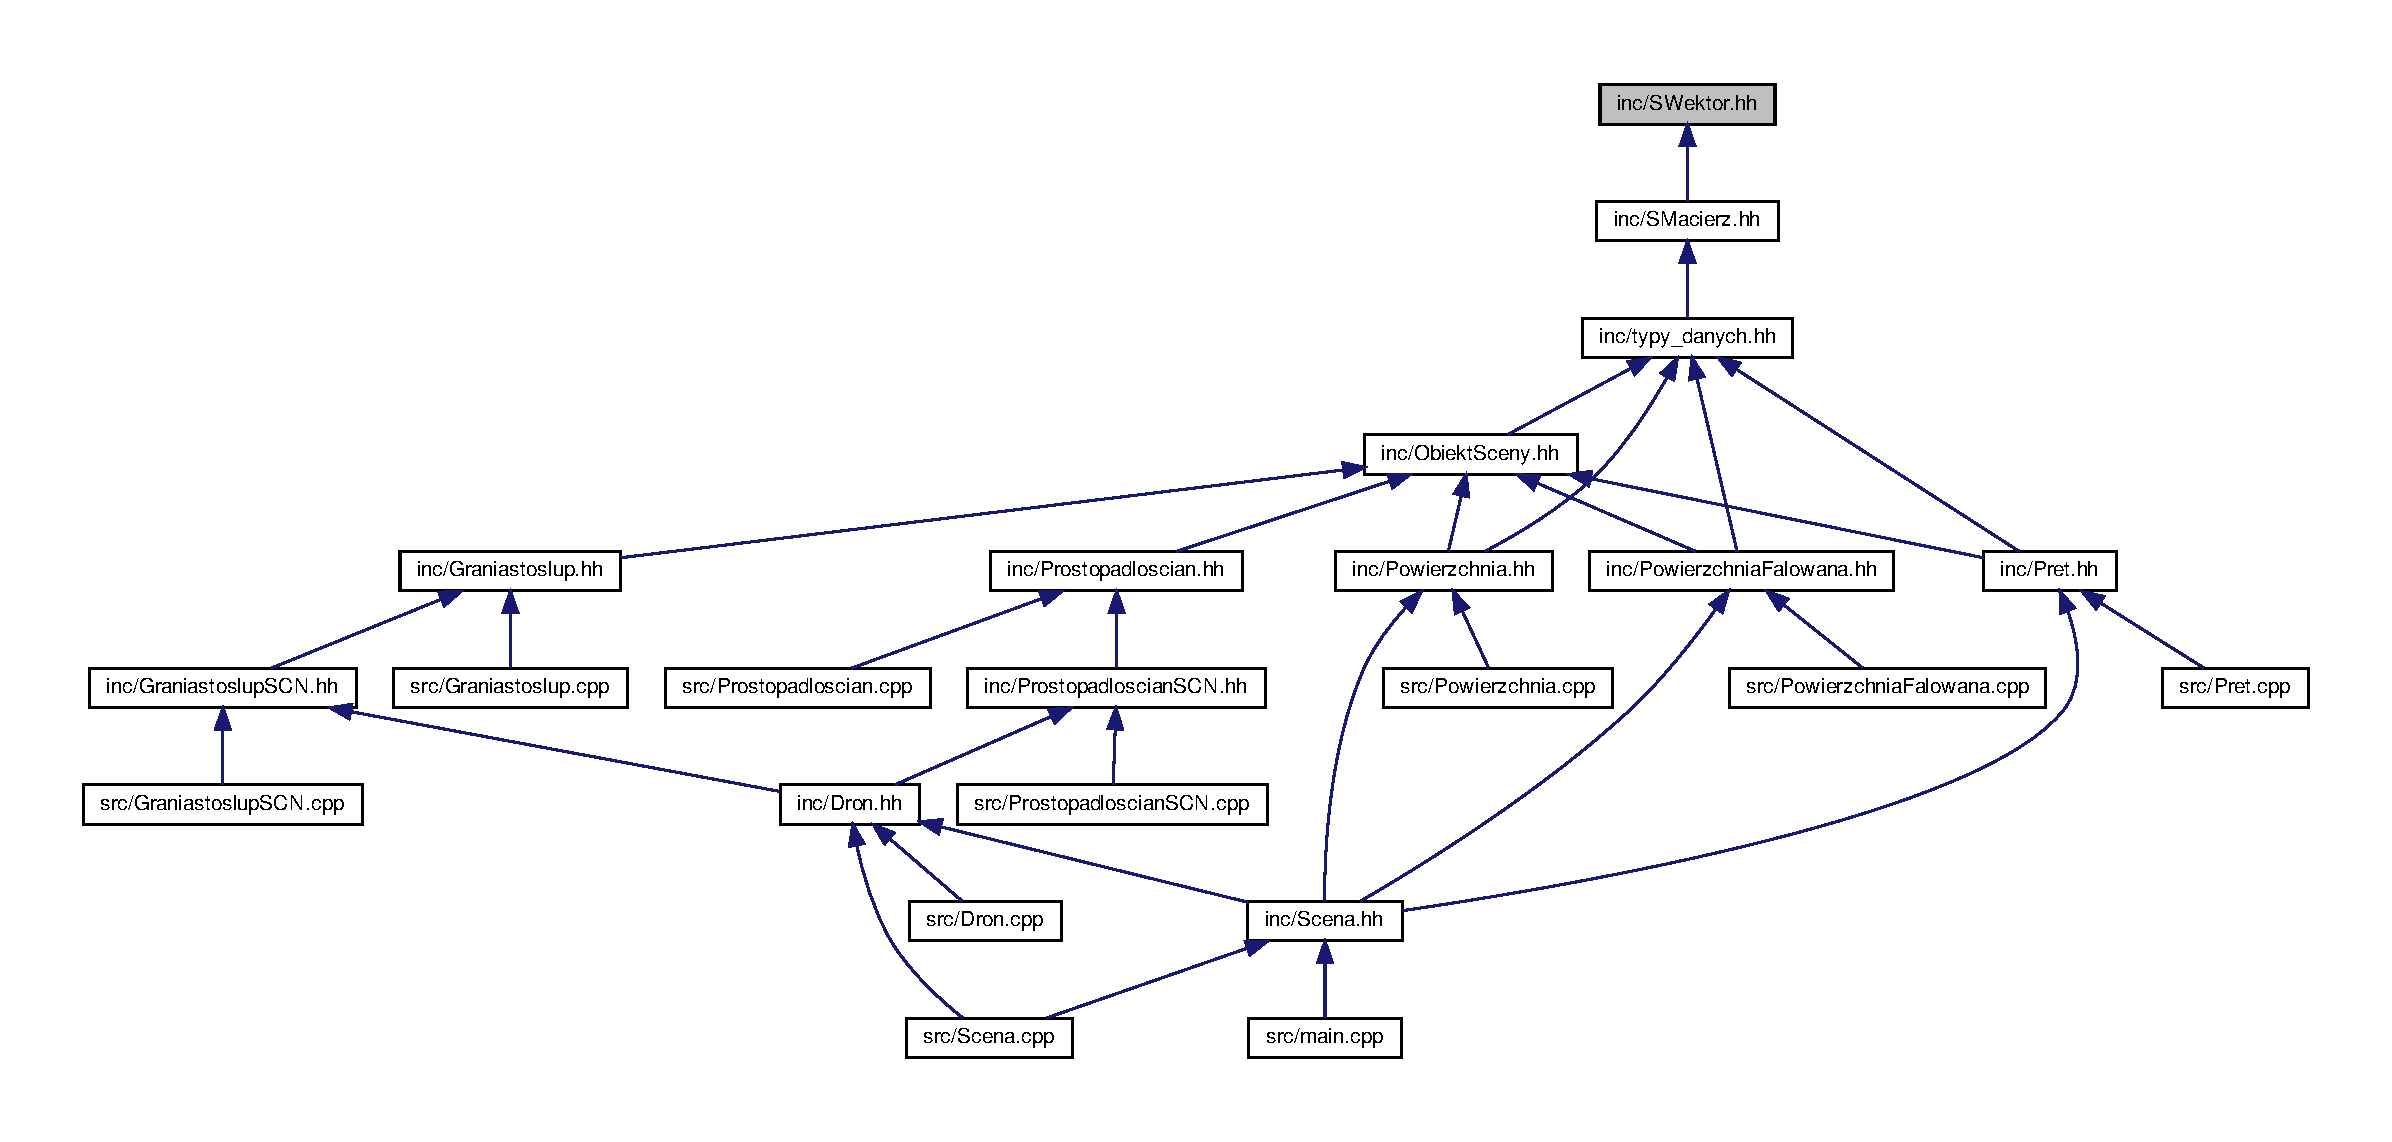
\includegraphics[width=350pt]{SWektor_8hh__dep__incl}
\end{center}
\end{figure}
\subsection*{Komponenty}
\begin{DoxyCompactItemize}
\item 
class \hyperlink{classSWektor}{S\+Wektor$<$ Typ, Wymiar $>$}
\begin{DoxyCompactList}\small\item\em Klasa modeluje pojecie wektora. \end{DoxyCompactList}\end{DoxyCompactItemize}
\subsection*{Funkcje}
\begin{DoxyCompactItemize}
\item 
{\footnotesize template$<$typename Typ , int Wymiar$>$ }\\std\+::ostream \& \hyperlink{SWektor_8hh_ac64bafa5b2d6cbab2daf26c794783b99}{operator$<$$<$} (std\+::ostream \&Strm\+Wy, const \hyperlink{classSWektor}{S\+Wektor}$<$ Typ, Wymiar $>$ \&Wek)
\item 
{\footnotesize template$<$typename Typ , int Wymiar$>$ }\\std\+::istream \& \hyperlink{SWektor_8hh_a3f97e20d3fc20a4fee82eb8515b49e94}{operator$>$$>$} (std\+::istream \&Strm\+We, \hyperlink{classSWektor}{S\+Wektor}$<$ Typ, Wymiar $>$ \&Wek)
\end{DoxyCompactItemize}


\subsection{Opis szczegółowy}
Plik zawiera szablon klasy modelujacej pojecie wektora. 

Plik zawiera szablon klasy modelujacej pojęcie wektora jako jednowymiarowej tablicy elementów double, o rozmiarze R\+O\+Z\+M\+I\+AR. Zawiera ona metody umożliwiające pobranie wartosci wybranego pola tablicy klasy, czy też jego modyfikację. Ponadto umożliwia wykonywanie działań arytmetycznych na wektorach, mnożenie i dzielenie wektora przez liczbę typu double, podanie długości wektora oraz przypisanie jednego wektora do drugiego. 

\subsection{Dokumentacja funkcji}
\mbox{\Hypertarget{SWektor_8hh_ac64bafa5b2d6cbab2daf26c794783b99}\label{SWektor_8hh_ac64bafa5b2d6cbab2daf26c794783b99}} 
\index{S\+Wektor.\+hh@{S\+Wektor.\+hh}!operator$<$$<$@{operator$<$$<$}}
\index{operator$<$$<$@{operator$<$$<$}!S\+Wektor.\+hh@{S\+Wektor.\+hh}}
\subsubsection{\texorpdfstring{operator$<$$<$()}{operator<<()}}
{\footnotesize\ttfamily template$<$typename Typ , int Wymiar$>$ \\
std\+::ostream\& operator$<$$<$ (\begin{DoxyParamCaption}\item[{std\+::ostream \&}]{Strm\+Wy,  }\item[{const \hyperlink{classSWektor}{S\+Wektor}$<$ Typ, Wymiar $>$ \&}]{Wek }\end{DoxyParamCaption})}

Realizuje wyswietlenie elementow wektora na strumien wyjsciowy. Argumenty\+: Srm\+We -\/ referencja do strumienia wejsciowego -\/ obiektu istream Wek -\/ referencja do stałego, wyswietlanego wektora -\/ obiektu klasy \hyperlink{classSWektor}{S\+Wektor} Zwraca\+: Referencje do strumienia wejsciowego \mbox{\Hypertarget{SWektor_8hh_a3f97e20d3fc20a4fee82eb8515b49e94}\label{SWektor_8hh_a3f97e20d3fc20a4fee82eb8515b49e94}} 
\index{S\+Wektor.\+hh@{S\+Wektor.\+hh}!operator$>$$>$@{operator$>$$>$}}
\index{operator$>$$>$@{operator$>$$>$}!S\+Wektor.\+hh@{S\+Wektor.\+hh}}
\subsubsection{\texorpdfstring{operator$>$$>$()}{operator>>()}}
{\footnotesize\ttfamily template$<$typename Typ , int Wymiar$>$ \\
std\+::istream\& operator$>$$>$ (\begin{DoxyParamCaption}\item[{std\+::istream \&}]{Strm\+We,  }\item[{\hyperlink{classSWektor}{S\+Wektor}$<$ Typ, Wymiar $>$ \&}]{Wek }\end{DoxyParamCaption})}

Wczytuje elementy wektora na podstawie danych ze strumienia wejsciowego. Argumenty\+: Srm\+We -\/ referencja do strumienia wejsciowego -\/ obiektu istream Wek -\/ referencja do wczytywanego wektora -\/ obiektu klasy \hyperlink{classSWektor}{S\+Wektor} Zwraca\+: Referencje do strumienia wejsciowego 
\hypertarget{typy__danych_8hh}{}\section{Dokumentacja pliku inc/typy\+\_\+danych.hh}
\label{typy__danych_8hh}\index{inc/typy\+\_\+danych.\+hh@{inc/typy\+\_\+danych.\+hh}}


Zawiera definicję Wektora3D oraz Macierzy3x3.  


{\ttfamily \#include \char`\"{}S\+Macierz.\+hh\char`\"{}}\newline
Wykres zależności załączania dla typy\+\_\+danych.\+hh\+:\nopagebreak
\begin{figure}[H]
\begin{center}
\leavevmode
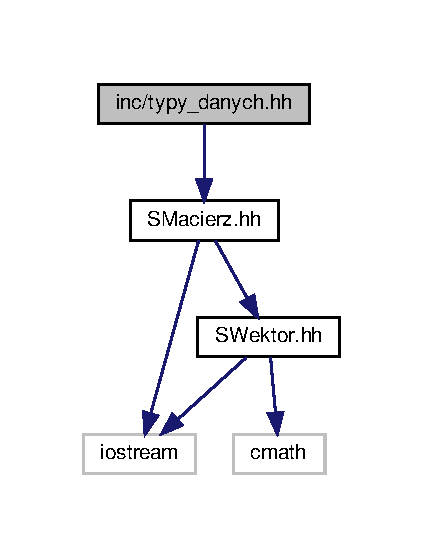
\includegraphics[width=203pt]{typy__danych_8hh__incl}
\end{center}
\end{figure}
Ten wykres pokazuje, które pliki bezpośrednio lub pośrednio załączają ten plik\+:\nopagebreak
\begin{figure}[H]
\begin{center}
\leavevmode
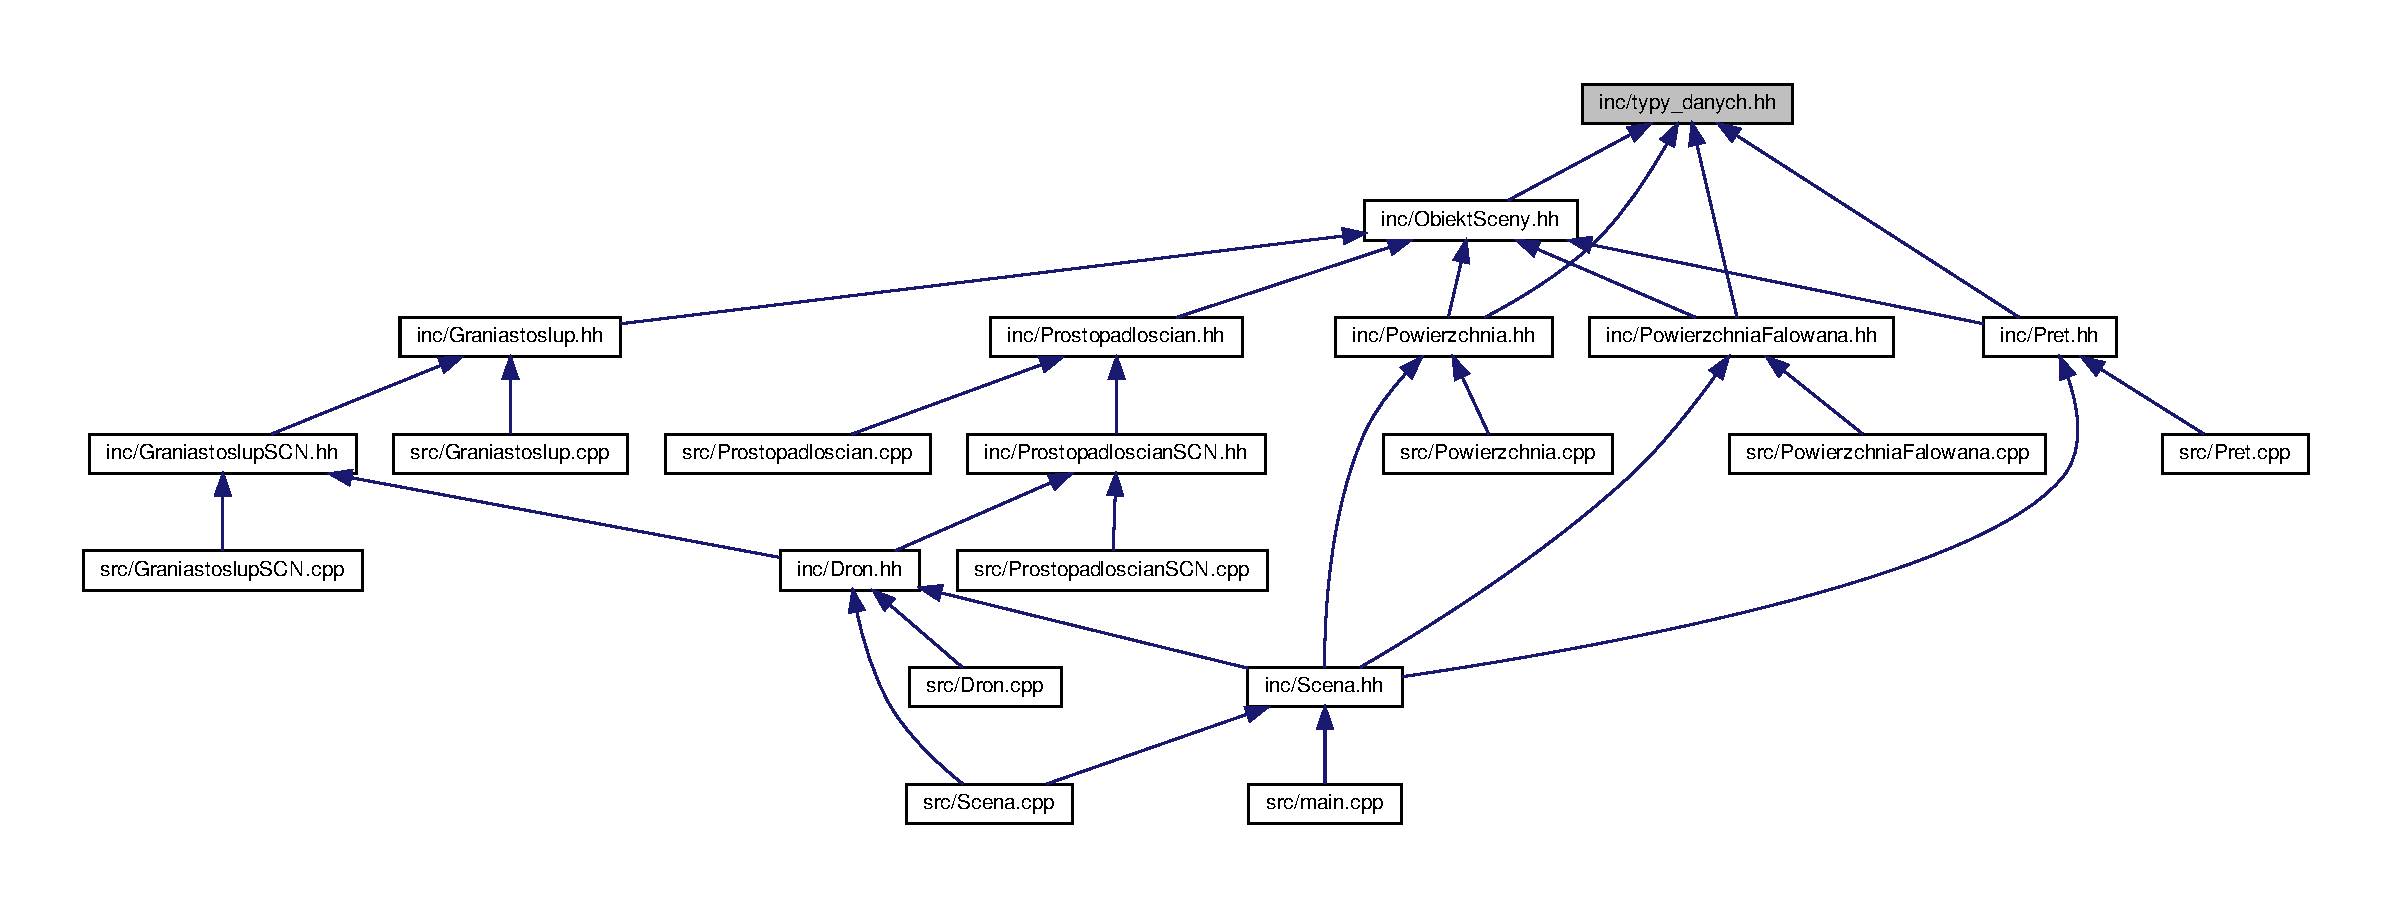
\includegraphics[width=350pt]{typy__danych_8hh__dep__incl}
\end{center}
\end{figure}
\subsection*{Definicje}
\begin{DoxyCompactItemize}
\item 
\mbox{\Hypertarget{typy__danych_8hh_a041a8dbff2d4eb4e4e7134a5f54406bf}\label{typy__danych_8hh_a041a8dbff2d4eb4e4e7134a5f54406bf}} 
\#define {\bfseries D\+O\+K\+L\+A\+D\+N\+O\+S\+C\+\_\+\+K\+A\+T\+A\+\_\+\+O\+D\+S\+W\+I\+E\+Z\+A\+N\+IA}~5
\item 
\mbox{\Hypertarget{typy__danych_8hh_a7f04bfdda9721d265bbb0d8063182abd}\label{typy__danych_8hh_a7f04bfdda9721d265bbb0d8063182abd}} 
\#define {\bfseries D\+O\+K\+L\+A\+D\+N\+O\+S\+C\+\_\+\+W\+E\+K\+T\+O\+R\+A\+\_\+\+O\+D\+S\+W\+I\+E\+Z\+A\+N\+IA}~5
\item 
\mbox{\Hypertarget{typy__danych_8hh_ac1623702b1fe474063b70d6fcd890184}\label{typy__danych_8hh_ac1623702b1fe474063b70d6fcd890184}} 
\#define {\bfseries C\+Z\+A\+S\+\_\+\+O\+D\+S\+W\+I\+E\+Z\+A\+N\+IA}~100000
\end{DoxyCompactItemize}
\subsection*{Definicje typów}
\begin{DoxyCompactItemize}
\item 
\mbox{\Hypertarget{typy__danych_8hh_a97a30d7257f40ddd7ba8726d98ba5c8b}\label{typy__danych_8hh_a97a30d7257f40ddd7ba8726d98ba5c8b}} 
typedef \hyperlink{classSWektor}{S\+Wektor}$<$ double, 3 $>$ {\bfseries Wektor3D}
\item 
\mbox{\Hypertarget{typy__danych_8hh_a8cb75ecee4b1f371170039dfe2ec4aa2}\label{typy__danych_8hh_a8cb75ecee4b1f371170039dfe2ec4aa2}} 
typedef \hyperlink{classSMacierz}{S\+Macierz}$<$ double, 3 $>$ {\bfseries Macierz3x3}
\end{DoxyCompactItemize}


\subsection{Opis szczegółowy}
Zawiera definicję Wektora3D oraz Macierzy3x3. 

Plik zawiera definicję Wektora3D jako obiektu \hyperlink{classSWektor}{S\+Wektor} o rozmiarze 3 z polami typu double oraz definicję Macierzy3x3 jako obiektu \hyperlink{classSMacierz}{S\+Macierz} o rozmiarze 3, składającego sie z wektorów o polach typu double. 
\hypertarget{Dron_8cpp}{}\section{Dokumentacja pliku src/\+Dron.cpp}
\label{Dron_8cpp}\index{src/\+Dron.\+cpp@{src/\+Dron.\+cpp}}


Zawiera definicje dluzszych metod klasy \hyperlink{classDron}{Dron}.  


{\ttfamily \#include \char`\"{}Dron.\+hh\char`\"{}}\newline
Wykres zależności załączania dla Dron.\+cpp\+:\nopagebreak
\begin{figure}[H]
\begin{center}
\leavevmode
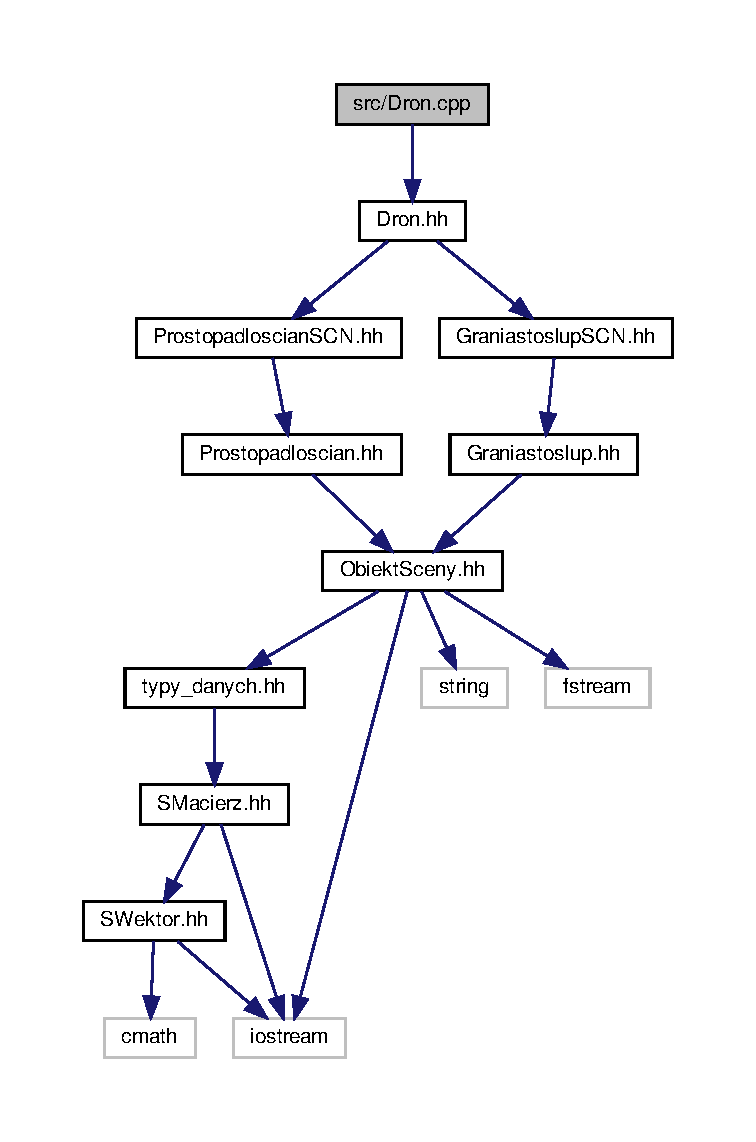
\includegraphics[width=350pt]{Dron_8cpp__incl}
\end{center}
\end{figure}


\subsection{Opis szczegółowy}
Zawiera definicje dluzszych metod klasy \hyperlink{classDron}{Dron}. 

Zawiera definicje dluzszych metod klasy \hyperlink{classDron}{Dron} 
\hypertarget{Graniastoslup_8cpp}{}\section{Dokumentacja pliku src/\+Graniastoslup.cpp}
\label{Graniastoslup_8cpp}\index{src/\+Graniastoslup.\+cpp@{src/\+Graniastoslup.\+cpp}}


Zawiera definicje dluzszych metod klasy \hyperlink{classGraniastoslup}{Graniastoslup}.  


{\ttfamily \#include \char`\"{}Graniastoslup.\+hh\char`\"{}}\newline
Wykres zależności załączania dla Graniastoslup.\+cpp\+:\nopagebreak
\begin{figure}[H]
\begin{center}
\leavevmode
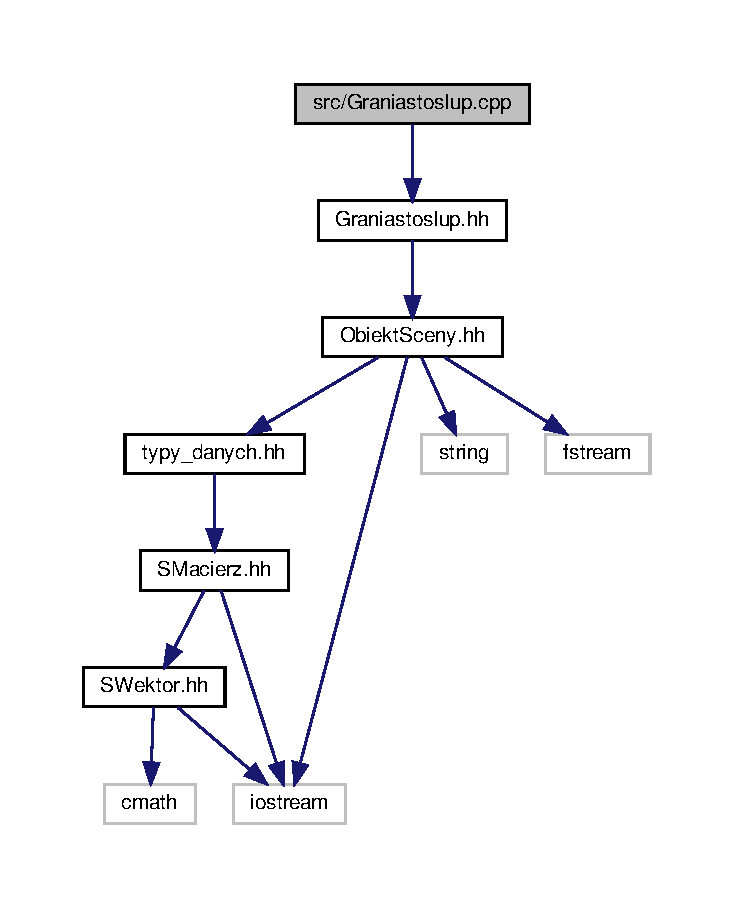
\includegraphics[width=350pt]{Graniastoslup_8cpp__incl}
\end{center}
\end{figure}


\subsection{Opis szczegółowy}
Zawiera definicje dluzszych metod klasy \hyperlink{classGraniastoslup}{Graniastoslup}. 

Zawiera definicje dluzszych metod klasy \hyperlink{classGraniastoslup}{Graniastoslup} 
\hypertarget{GraniastoslupSCN_8cpp}{}\section{Dokumentacja pliku src/\+Graniastoslup\+S\+CN.cpp}
\label{GraniastoslupSCN_8cpp}\index{src/\+Graniastoslup\+S\+C\+N.\+cpp@{src/\+Graniastoslup\+S\+C\+N.\+cpp}}


Zawiera definicje dluzszych metod klasy \hyperlink{classGraniastoslupSCN}{Graniastoslup\+S\+CN}.  


{\ttfamily \#include \char`\"{}Graniastoslup\+S\+C\+N.\+hh\char`\"{}}\newline
Wykres zależności załączania dla Graniastoslup\+S\+C\+N.\+cpp\+:\nopagebreak
\begin{figure}[H]
\begin{center}
\leavevmode
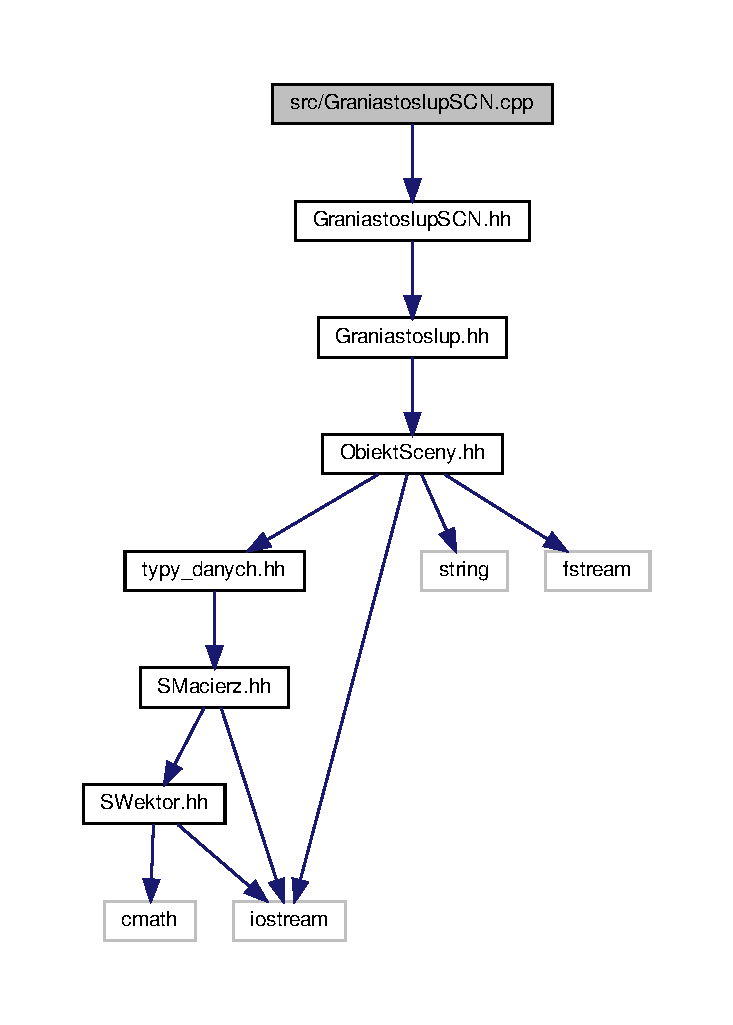
\includegraphics[width=350pt]{GraniastoslupSCN_8cpp__incl}
\end{center}
\end{figure}


\subsection{Opis szczegółowy}
Zawiera definicje dluzszych metod klasy \hyperlink{classGraniastoslupSCN}{Graniastoslup\+S\+CN}. 

Zawiera definicje dluzszych metod klasy \hyperlink{classGraniastoslupSCN}{Graniastoslup\+S\+CN} 
\hypertarget{lacze__do__gnuplota_8cpp}{}\section{Dokumentacja pliku src/lacze\+\_\+do\+\_\+gnuplota.cpp}
\label{lacze__do__gnuplota_8cpp}\index{src/lacze\+\_\+do\+\_\+gnuplota.\+cpp@{src/lacze\+\_\+do\+\_\+gnuplota.\+cpp}}


Zawiera definicje metod klasy Lacze\+Do\+G\+N\+U\+Plota.  


{\ttfamily \#include $<$cstdlib$>$}\newline
{\ttfamily \#include $<$cstdio$>$}\newline
{\ttfamily \#include $<$cstring$>$}\newline
{\ttfamily \#include $<$cmath$>$}\newline
{\ttfamily \#include $<$iostream$>$}\newline
{\ttfamily \#include $<$sys/stat.\+h$>$}\newline
{\ttfamily \#include $<$unistd.\+h$>$}\newline
{\ttfamily \#include $<$fcntl.\+h$>$}\newline
{\ttfamily \#include $<$sstream$>$}\newline
{\ttfamily \#include \char`\"{}lacze\+\_\+do\+\_\+gnuplota.\+hh\char`\"{}}\newline
Wykres zależności załączania dla lacze\+\_\+do\+\_\+gnuplota.\+cpp\+:\nopagebreak
\begin{figure}[H]
\begin{center}
\leavevmode
\includegraphics[width=350pt]{lacze__do__gnuplota_8cpp__incl}
\end{center}
\end{figure}
\subsection*{Przestrzenie nazw}
\begin{DoxyCompactItemize}
\item 
 \hyperlink{namespacePzG}{PzG}
\begin{DoxyCompactList}\small\item\em Moduł narzędzi umożliwiających połącznie z G\+N\+U\+Plotem. \end{DoxyCompactList}\end{DoxyCompactItemize}
\subsection*{Definicje}
\begin{DoxyCompactItemize}
\item 
\mbox{\Hypertarget{lacze__do__gnuplota_8cpp_ac00bfb46347d26fdc58568fe1ab5fa5b}\label{lacze__do__gnuplota_8cpp_ac00bfb46347d26fdc58568fe1ab5fa5b}} 
\#define {\bfseries S\+T\+D\+IN}~0
\item 
\mbox{\Hypertarget{lacze__do__gnuplota_8cpp_a8875037d0772a4fc34516f1e03d7e238}\label{lacze__do__gnuplota_8cpp_a8875037d0772a4fc34516f1e03d7e238}} 
\#define {\bfseries S\+T\+D\+O\+UT}~1
\item 
\mbox{\Hypertarget{lacze__do__gnuplota_8cpp_a2b501945c8d86114fcf6420cc1ee6306}\label{lacze__do__gnuplota_8cpp_a2b501945c8d86114fcf6420cc1ee6306}} 
\#define {\bfseries R\+O\+Z\+\_\+\+L\+I\+N\+II}~120
\end{DoxyCompactItemize}
\subsection*{Funkcje}
\begin{DoxyCompactItemize}
\item 
\mbox{\Hypertarget{namespacePzG_ae1ae4d36f66c77879380ba73da8e20e3}\label{namespacePzG_ae1ae4d36f66c77879380ba73da8e20e3}} 
bool {\bfseries Pz\+G\+::\+Czy\+Jest\+Plik} (char const $\ast$Nazwa\+Pliku)
\end{DoxyCompactItemize}


\subsection{Opis szczegółowy}
Zawiera definicje metod klasy Lacze\+Do\+G\+N\+U\+Plota. 

Zawiera definicje metod klasy Lacze\+Do\+G\+N\+U\+Plota wraz z ich opisem. 
\hypertarget{main_8cpp}{}\section{Dokumentacja pliku src/main.cpp}
\label{main_8cpp}\index{src/main.\+cpp@{src/main.\+cpp}}


Zawiera funkcje main.  


{\ttfamily \#include $<$iomanip$>$}\newline
{\ttfamily \#include \char`\"{}Scena.\+hh\char`\"{}}\newline
Wykres zależności załączania dla main.\+cpp\+:\nopagebreak
\begin{figure}[H]
\begin{center}
\leavevmode
\includegraphics[width=350pt]{main_8cpp__incl}
\end{center}
\end{figure}
\subsection*{Funkcje}
\begin{DoxyCompactItemize}
\item 
\mbox{\Hypertarget{main_8cpp_ae66f6b31b5ad750f1fe042a706a4e3d4}\label{main_8cpp_ae66f6b31b5ad750f1fe042a706a4e3d4}} 
int {\bfseries main} ()
\end{DoxyCompactItemize}


\subsection{Opis szczegółowy}
Zawiera funkcje main. 

Plik zawiera kod zrodlowy funkcji main sterujacej przeplywem programu. Program rozpoczyna swoje dzialanie inicjalizacja sceny, powodujacej narysowanie stanu poczatkowego obiektow. Nastepnie udostepnia menu uzytkownika, za pomoca ktorego uzytkownik moze nakazac dronowi wykonac ruch do przodu z okreslolnym katem opadania lub obrot wokol osi OZ. Kazda z tych czynnosci jest odpowiednio animowana na scenie.


\begin{DoxyRetVals}{Zwracane wartości}
{\em -\/1} & -\/ Niepoprawna inicjalizacja sceny \\
\hline
{\em 0} & -\/ Program wszystkie operacje wykonal poprawnie \\
\hline
\end{DoxyRetVals}

\hypertarget{Powierzchnia_8cpp}{}\section{Dokumentacja pliku src/\+Powierzchnia.cpp}
\label{Powierzchnia_8cpp}\index{src/\+Powierzchnia.\+cpp@{src/\+Powierzchnia.\+cpp}}


Zawiera definicje dluzszych metod klasy \hyperlink{classPowierzchnia}{Powierzchnia}.  


{\ttfamily \#include \char`\"{}Powierzchnia.\+hh\char`\"{}}\newline
Wykres zależności załączania dla Powierzchnia.\+cpp\+:\nopagebreak
\begin{figure}[H]
\begin{center}
\leavevmode
\includegraphics[width=314pt]{Powierzchnia_8cpp__incl}
\end{center}
\end{figure}


\subsection{Opis szczegółowy}
Zawiera definicje dluzszych metod klasy \hyperlink{classPowierzchnia}{Powierzchnia}. 

Zawiera definicje dluzszych metod klasy \hyperlink{classPowierzchnia}{Powierzchnia} 
\hypertarget{PowierzchniaFalowana_8cpp}{}\section{Dokumentacja pliku src/\+Powierzchnia\+Falowana.cpp}
\label{PowierzchniaFalowana_8cpp}\index{src/\+Powierzchnia\+Falowana.\+cpp@{src/\+Powierzchnia\+Falowana.\+cpp}}


Zawiera definicje dluzszych metod klasy \hyperlink{classPowierzchniaFalowana}{Powierzchnia\+Falowana}.  


{\ttfamily \#include \char`\"{}Powierzchnia\+Falowana.\+hh\char`\"{}}\newline
Wykres zależności załączania dla Powierzchnia\+Falowana.\+cpp\+:\nopagebreak
\begin{figure}[H]
\begin{center}
\leavevmode
\includegraphics[width=314pt]{PowierzchniaFalowana_8cpp__incl}
\end{center}
\end{figure}


\subsection{Opis szczegółowy}
Zawiera definicje dluzszych metod klasy \hyperlink{classPowierzchniaFalowana}{Powierzchnia\+Falowana}. 

Zawiera definicje dluzszych metod klasy \hyperlink{classPowierzchniaFalowana}{Powierzchnia\+Falowana} 
\hypertarget{Pret_8cpp}{}\section{Dokumentacja pliku src/\+Pret.cpp}
\label{Pret_8cpp}\index{src/\+Pret.\+cpp@{src/\+Pret.\+cpp}}


Zawiera definicje dluzszych metod klasy \hyperlink{classPret}{Pret}.  


{\ttfamily \#include \char`\"{}Pret.\+hh\char`\"{}}\newline
Wykres zależności załączania dla Pret.\+cpp\+:\nopagebreak
\begin{figure}[H]
\begin{center}
\leavevmode
\includegraphics[width=314pt]{Pret_8cpp__incl}
\end{center}
\end{figure}


\subsection{Opis szczegółowy}
Zawiera definicje dluzszych metod klasy \hyperlink{classPret}{Pret}. 

Zawiera definicje dluzszych metod klasy \hyperlink{classPret}{Pret} 
\hypertarget{Prostopadloscian_8cpp}{}\section{Dokumentacja pliku src/\+Prostopadloscian.cpp}
\label{Prostopadloscian_8cpp}\index{src/\+Prostopadloscian.\+cpp@{src/\+Prostopadloscian.\+cpp}}


Zawiera definicje dluzszych metod klasy \hyperlink{classProstopadloscian}{Prostopadloscian}.  


{\ttfamily \#include \char`\"{}Prostopadloscian.\+hh\char`\"{}}\newline
Wykres zależności załączania dla Prostopadloscian.\+cpp\+:\nopagebreak
\begin{figure}[H]
\begin{center}
\leavevmode
\includegraphics[width=350pt]{Prostopadloscian_8cpp__incl}
\end{center}
\end{figure}


\subsection{Opis szczegółowy}
Zawiera definicje dluzszych metod klasy \hyperlink{classProstopadloscian}{Prostopadloscian}. 

Zawiera definicje dluzszych metod klasy \hyperlink{classProstopadloscian}{Prostopadloscian} 
\hypertarget{ProstopadloscianSCN_8cpp}{}\section{Dokumentacja pliku src/\+Prostopadloscian\+S\+CN.cpp}
\label{ProstopadloscianSCN_8cpp}\index{src/\+Prostopadloscian\+S\+C\+N.\+cpp@{src/\+Prostopadloscian\+S\+C\+N.\+cpp}}


Zawiera definicje dluzszych metod klasy \hyperlink{classProstopadloscianSCN}{Prostopadloscian\+S\+CN}.  


{\ttfamily \#include \char`\"{}Prostopadloscian\+S\+C\+N.\+hh\char`\"{}}\newline
Wykres zależności załączania dla Prostopadloscian\+S\+C\+N.\+cpp\+:\nopagebreak
\begin{figure}[H]
\begin{center}
\leavevmode
\includegraphics[width=350pt]{ProstopadloscianSCN_8cpp__incl}
\end{center}
\end{figure}


\subsection{Opis szczegółowy}
Zawiera definicje dluzszych metod klasy \hyperlink{classProstopadloscianSCN}{Prostopadloscian\+S\+CN}. 

Zawiera definicje dluzszych metod klasy \hyperlink{classProstopadloscianSCN}{Prostopadloscian\+S\+CN} 
\hypertarget{Scena_8cpp}{}\section{Dokumentacja pliku src/\+Scena.cpp}
\label{Scena_8cpp}\index{src/\+Scena.\+cpp@{src/\+Scena.\+cpp}}


Zawiera definicje dluzszych metod klasy \hyperlink{classScena}{Scena}.  


{\ttfamily \#include \char`\"{}Scena.\+hh\char`\"{}}\newline
{\ttfamily \#include \char`\"{}Dron.\+hh\char`\"{}}\newline
Wykres zależności załączania dla Scena.\+cpp\+:\nopagebreak
\begin{figure}[H]
\begin{center}
\leavevmode
\includegraphics[width=350pt]{Scena_8cpp__incl}
\end{center}
\end{figure}


\subsection{Opis szczegółowy}
Zawiera definicje dluzszych metod klasy \hyperlink{classScena}{Scena}. 

Zawiera definicje dluzszych metod klasy \hyperlink{classScena}{Scena} 
%--- End generated contents ---

% Index
\backmatter
\newpage
\phantomsection
\clearemptydoublepage
\addcontentsline{toc}{chapter}{Indeks}
\printindex

\end{document}
